\documentclass[a4paper,11pt]{book}
%\documentclass[a4paper,twoside,11pt,titlepage]{book}
\usepackage{listings}
\usepackage[utf8]{inputenc}
\usepackage[spanish,es-tabla]{babel}

\usepackage{textcomp}
\usepackage{multirow}
\usepackage[table,xcdraw]{xcolor}

% \usepackage[style=list, number=none]{glossary} %
%\usepackage{titlesec}
%\usepackage{pailatino}

\decimalpoint
\usepackage{dcolumn}
\newcolumntype{.}{D{.}{\esperiod}{-1}}
\makeatletter
\addto\shorthandsspanish{\let\esperiod\es@period@code}
\makeatother


%\usepackage[chapter]{algorithm}
\RequirePackage{verbatim}
%\RequirePackage[Glenn]{fncychap}
\usepackage{fancyhdr}
\usepackage{graphicx}
\usepackage{afterpage}

\usepackage{longtable}

%\usepackage[pdfborder={000}]{hyperref} %referencia
\usepackage[colorlinks=true,urlcolor=blue,linkcolor=red]{hyperref}

% ********************************************************************
% Re-usable information
% ********************************************************************
\newcommand{\myTitle}{Diseño de Metaheurística para problemas combinatorios costosos\xspace}
\newcommand{\myDegree}{Doble Grado en Ingeniería Informática y Matemáticas\xspace}
\newcommand{\myName}{Irene Trigueros Lorca\xspace}
\newcommand{\myProf}{Daniel Molina Cabrera\xspace}
\newcommand{\myOtherProf}{Francisco Herrera Triguero\xspace}
%\newcommand{\mySupervisor}{Put name here\xspace}
\newcommand{\myFaculty}{Escuela Técnica Superior de Ingenierías Informática y de
Telecomunicación\\Facultad de Ciencias\xspace}
\newcommand{\myFacultyShort}{E.T.S. de Ingenierías Informática y de
Telecomunicación\\Facultad de Ciencias\xspace}
\newcommand{\myDepartment}{Departamento de ...\xspace}
\newcommand{\myUni}{\protect{Universidad de Granada}\xspace}
\newcommand{\myLocation}{Granada\xspace}
\newcommand{\myTime}{\today\xspace}
\newcommand{\myVersion}{Version 0.1\xspace}


\hypersetup{
pdfauthor = {\myName irenetrigueros@correo.ugr.es},
pdftitle = {\myTitle},
pdfsubject = {},
pdfkeywords = {palabra_clave1, palabra_clave2, palabra_clave3, ...},
pdfcreator = {LaTeX con el paquete ....},
pdfproducer = {pdflatex}
}

%\hyphenation{}


%\usepackage{doxygen/doxygen}
%\usepackage{pdfpages}
\usepackage{url}
\usepackage{colortbl,longtable}
\usepackage[stable]{footmisc}
%\usepackage{index}

%\makeindex
%\usepackage[style=long, cols=2,border=plain,toc=true,number=none]{glossary}
% \makeglossary

% Definición de comandos que me son tiles:
%\renewcommand{\indexname}{Índice alfabético}
%\renewcommand{\glossaryname}{Glosario}

\pagestyle{fancy}
\fancyhf{}
\fancyhead[LO]{\leftmark}
\fancyhead[RE]{\rightmark}
\fancyhead[RO,LE]{\textbf{\thepage}}
\renewcommand{\chaptermark}[1]{\markboth{\textbf{#1}}{}}
\renewcommand{\sectionmark}[1]{\markright{\textbf{\thesection. #1}}}

%\setlength{\headheight}{1.5\headheight}

\newcommand{\HRule}{\rule{\linewidth}{0.5mm}}
%Definimos los tipos teorema, ejemplo y definición podremos usar estos tipos
%simplemente poniendo \begin{teorema} \end{teorema} ...
\newtheorem{teorema}{Teorema}[chapter]
\newtheorem{ejemplo}{Ejemplo}[chapter]
\newtheorem{definicion}{Definición}[chapter]
\newtheorem{proposicion}{Proposición}[chapter]

\definecolor{gray97}{gray}{.97}
\definecolor{gray75}{gray}{.75}
\definecolor{gray45}{gray}{.45}
\definecolor{gray30}{gray}{.94}

\lstset{ frame=Ltb,
     framerule=0.5pt,
     aboveskip=0.5cm,
     framextopmargin=3pt,
     framexbottommargin=3pt,
     framexleftmargin=0.1cm,
     framesep=0pt,
     rulesep=.4pt,
     backgroundcolor=\color{gray97},
     rulesepcolor=\color{black},
     %
     stringstyle=\ttfamily,
     showstringspaces = false,
     basicstyle=\scriptsize\ttfamily,
     commentstyle=\color{gray45},
     keywordstyle=\bfseries,
     %
     numbers=left,
     numbersep=6pt,
     numberstyle=\tiny,
     numberfirstline = false,
     breaklines=true,
   }
 
% minimizar fragmentado de listados
\lstnewenvironment{listing}[1][]
   {\lstset{#1}\pagebreak[0]}{\pagebreak[0]}

\lstdefinestyle{CodigoC}
   {
	basicstyle=\scriptsize,
	frame=single,
	language=C,
	numbers=left
   }
\lstdefinestyle{CodigoC++}
   {
	basicstyle=\small,
	frame=single,
	backgroundcolor=\color{gray30},
	language=C++,
	numbers=left
   }

 
\lstdefinestyle{Consola}
   {basicstyle=\scriptsize\bf\ttfamily,
    backgroundcolor=\color{gray30},
    frame=single,
    numbers=none
   }


\newcommand{\bigrule}{\titlerule[0.5mm]}

%Para que el número de capítulo y el título estén en la misma línea
\usepackage{titlesec}
\titleformat{\chapter}[hang] 
{\normalfont\huge\bfseries}{\chaptertitlename\ \thechapter:}{1em}{} 

%Para conseguir que en las páginas en blanco no ponga cabecerass
\makeatletter
\def\clearpage{%
  \ifvmode
    \ifnum \@dbltopnum =\m@ne
      \ifdim \pagetotal <\topskip
        \hbox{}
      \fi
    \fi
  \fi
  \newpage
  \thispagestyle{empty}
  \write\m@ne{}
  \vbox{}
  \penalty -\@Mi
}
\makeatother

\usepackage{lmodern}
\usepackage[T1]{fontenc}
\usepackage{mathtools}
\usepackage{vmargin}
\usepackage{caption}
\usepackage{subcaption}
\usepackage{float}
\usepackage{amsmath}
\usepackage{amsfonts}
\usepackage{amssymb}
\usepackage{enumerate}
\usepackage{schemata}
\usepackage{hyperref}
\usepackage{enumitem}
\usepackage[all]{hypcap}    %for going to the top of an image when a figure reference is clicked
\newcommand\diagram[2]{\schema{\schemabox{#1}}{\schemabox{#2}}}
\usepackage{xspace}
\usepackage{algorithm}
\usepackage{algpseudocode}
\usepackage{cleveref}
\usepackage[style=ieee,maxnames=10]{biblatex}
\AtEveryBibitem{%
  \clearfield{note}%
}
\addbibresource{TFG.bib}

\usepackage{float}
\floatstyle{plaintop}
\restylefloat{table}
\usepackage[paper=portrait,pagesize]{typearea}

\algnewcommand\algorithmicforeach{\textbf{for each}}
\algdef{S}[FOR]{ForEach}[1]{\algorithmicforeach\ #1\ \algorithmicdo}


\setlength{\parskip}{0.5em}

\setpapersize{A4}
\setmargins{2.25cm}       % margen izquierdo
{1.5cm}                        % margen superior
{16.5cm}                      % anchura del texto
{23.42cm}                    % altura del texto
{10pt}                           % altura de los encabezados
{1cm}                           % espacio entre el texto y los encabezados
{0pt}                             % altura del pie de página
{2cm}                           % espacio entre el texto y el pie de página
\usepackage{pdfpages}
%\usepackage[a4paper,left=2.25cm,right=2.25cm,top=1.5cm,bottom=1.5cm]{geometry}
\begin{document}
\begin{titlepage}
 
 
\newlength{\centeroffset}
\setlength{\centeroffset}{-0.5\oddsidemargin}
\addtolength{\centeroffset}{0.5\evensidemargin}
\thispagestyle{empty}

\noindent\hspace*{\centeroffset}\begin{minipage}{\textwidth}

\centering

\includegraphics[width=0.8\textwidth]{imagenes/logo_ugr.jpg}\\[1.4cm]

\textsc{ \Large TRABAJO FIN DE GRADO\\[0.2cm]}
\textsc{ DOBLE GRADO EN INGENIERÍA INFORMÁTICA Y MATEMÁTICAS}\\[1cm]
% Upper part of the page
% 
% Title
{\Huge\bfseries Diseño de Metaheurística para problemas combinatorios costosos\\
}
\noindent\rule[-1ex]{\textwidth}{3pt}\\[3.5ex]
%{\large\bfseries Subtitulo del Proyecto}
\end{minipage}

\vspace{1cm}
\noindent\hspace*{\centeroffset}\begin{minipage}{\textwidth}
\centering

\textbf{Autor}\\ {Irene Trigueros Lorca}\\[2.5ex]
\textbf{Directores}\\
{Daniel Molina Cabrera\\
Francisco Herrera Triguero}\\[1cm]

\begin{tabular}{c c}

\includegraphics[scale=1]{imagenes/etsiit_logo.png} & 
\includegraphics[scale=0.2]{imagenes/ciencias_logo.png}\\
\textsc{Escuela Técnica Superior de}\\\textsc{Ingenierías Informática}\\\textsc{y de Telecomunicación} & \textsc{Facultad de Ciencias} \\
\end{tabular} 

%
\includegraphics[width=0.3\textwidth]{imagenes/etsiit_logo.png}\\[0.1cm]
%\textsc{Escuela Técnica Superior de Ingenierías Informática y de Telecomunicación}\\
\textsc{---}\\
Granada, Mayo de 2023
\end{minipage}
%\addtolength{\textwidth}{\centeroffset}
%\vspace{\stretch{2}}
\end{titlepage}



\chapter*{}
%\thispagestyle{empty}
%\cleardoublepage

%\thispagestyle{empty}

\begin{titlepage}
 
 
\setlength{\centeroffset}{-0.5\oddsidemargin}
\addtolength{\centeroffset}{0.5\evensidemargin}
\thispagestyle{empty}

\noindent\hspace*{\centeroffset}\begin{minipage}{\textwidth}

\centering
%
\includegraphics[width=0.9\textwidth]{imagenes/logo_ugr.jpg}\\[1.4cm]

%\textsc{ \Large PROYECTO FIN DE CARRERA\\[0.2cm]}
%\textsc{ INGENIERÍA EN INFORMÁTICA}\\[1cm]
% Upper part of the page
% 

 \vspace{3.3cm}

%si el proyecto tiene logo poner aquí

\includegraphics[width=0.8\textwidth]{imagenes/logo_ugr_nuevo.png} 
 \vspace{0.5cm}

% Title

{\Huge\bfseries Diseño de Metaheurística para problemas combinatorios costosos\\
}
\noindent\rule[-1ex]{\textwidth}{3pt}\\[3.5ex]
%{\large\bfseries Subtítulo del proyecto.\\[4cm]}
\end{minipage}

\vspace{2.5cm}
\noindent\hspace*{\centeroffset}\begin{minipage}{\textwidth}
\centering

\textbf{Autor}\\ {Irene Trigueros Lorca}\\[2.5ex]
\textbf{Directores}\\
{Daniel Molina Cabrera\\
Francisco Herrera Triguero}\\[2cm]
%
\includegraphics[width=0.15\textwidth]{imagenes/tstc.png}\\[0.1cm]
%\textsc{Departamento de Teoría de la Señal, Telemática y Comunicaciones}\\
%\textsc{---}\\
%Granada, mes de 201
\end{minipage}
%\addtolength{\textwidth}{\centeroffset}
\vspace{\stretch{2}}

 
\end{titlepage}






\cleardoublepage
\thispagestyle{empty}

\begin{center}
{\large\bfseries Diseño de Metaheurística para problemas combinatorios costosos}\\
\end{center}
\begin{center}
Irene Trigueros Lorca\\
\end{center}

%\vspace{0.7cm}
\noindent{\textbf{Palabras clave}: metaheurística, combinatorio, costoso, optimización, algoritmo genético, exploración, explotación, diversidad}\\

\vspace{0.7cm}
\noindent{\textbf{Resumen}}\\

Existen problemas de mucho interés cuyo coste de evaluación es excesivamente elevado (a este tipo de problemas los llamaremos problemas costosos o problemas \textit{expensive}), como podrían ser los problemas de optimización de redes neuronales, por lo que resulta interesante desarrollar algoritmos capaces de obtener soluciones competitivas en muy pocas evaluaciones. 
Además, en la literatura ya encontramos algoritmos específicos en problemas \textit{expensives} de optimización continua; pero no ocurre lo mismo con el caso de problemas combinatorios, para los que no se han hallado ningún algoritmo capaz de resolverlos.

Por lo tanto, en este proyecto se propone un algoritmo metaheurístico nuevo para resolver problemas combinatorios costosos (\textit{expensive}), siguiendo un formato semejante al de un diario de desarrollo. 
Se tomará como algoritmo base un algoritmo genético y, una vez analizado su rendimiento, se implementarán una serie de modificaciones que, progresivamente, compondrán la versión final del algoritmo. 
Estas modificaciones se justificarán observando y analizando los resultados obtenidos en los intentos anteriores con el objetivo de encontrar formas de aprovechar al máximo las pocas evaluaciones que nos podemos permitir en este tipo de problemas. 
Se describen detalladamente las tareas adicionales llevadas a cabo propias del desarrollo de un algoritmo de esta clase. 
%Además, se realizan análisis experimentales donde se compara el algoritmo base y las sucesivas versiones del algoritmo a crear. 
Además, se realizarán análisis experimentales que irán demostrando que las sucesivas versiones del algoritmo van mejorando las anteriores.
Las conclusiones que se alcanzan indican que el algoritmo presentado en este proyecto es altamente competitivo. 



\cleardoublepage


\thispagestyle{empty}


\begin{center}
{\large\bfseries Metaheuristics design for expensive combinatorial problems }\\
\end{center}
\begin{center}
Irene Trigueros Lorca\\
\end{center}

%\vspace{0.7cm}
\noindent{\textbf{Keywords}: metaheuristic, combinatory, expensive, optimization, genetic algorithm, exploration, explotation, diversity}\\

\vspace{0.7cm}
\noindent{\textbf{Abstract}}\\

There are very interesting problems which their computational cost is excessively high (these kind of problems will be refered as expensive problems), such as the neural network optimization problems, therefore it is compelling to develope algorithms that are able to obtain competitive solutions in few evaluations. 
Furthermore, specific algorithms for the optimization of expensive continous problems can be found in the literature; but that is not the case for the combinatory expensive problems, for those which no algorithms able to solve them have been found.

Hence, throughout this project, an original metaheuristic algorithm is going to be proposed with the purpose of solving expensive problems, following a format similar to that of a developer diary. 
A genetic algorithm is going to be chosen as the base algorithm and, once its performance is analyzed, a series of modifications are going  to be implemented, which, at the end, will compose the final version of the algorithm. 
These modifications are going to be justified by observing and analyzing the results obtained through the previous attempts with the objective of finding ways of making the most of the few iterations available in these kind of problems. 
Additional tasks regarding the development of this type of algorithms are described in depth. 
Furthermore, experimental analysis is included, where both base and the following versions algorithms are compared. 
The final conclusions suggest that the algorithm presented within this project is highly performant.

\chapter*{}
\thispagestyle{empty}

\noindent\rule[-1ex]{\textwidth}{2pt}\\[4.5ex]

Yo, \textbf{Irene Trigueros Lorca}, alumno de la titulación Doble Grado en Ingeniería Informática y Matemáticas de la \textbf{Escuela Técnica Superior
de Ingenierías Informática y de Telecomunicación de la Universidad de Granada} y de la \textbf{Facultad de Ciencias}, con DNI 77385991F, autorizo la
ubicación de la siguiente copia de mi Trabajo Fin de Grado en la biblioteca de ambos centro para que pueda ser
consultada por las personas que lo deseen.

\vspace{6cm}

\noindent Fdo: Irene Trigueros Lorca

\vspace{2cm}

\begin{flushright}
Granada a, \today.
\end{flushright}


\chapter*{}
\thispagestyle{empty}

\noindent\rule[-1ex]{\textwidth}{2pt}\\[4.5ex]

D. \textbf{Daniel Molina Cabrera}, Profesor del Departamento Ciencias de la Computación e Inteligencia Artificial de la Universidad de Granada.

\vspace{0.5cm}

D. \textbf{Francisco Herrera Triguero}, Profesor del Departamento Ciencias de la Computación e Inteligencia Artificial de la Universidad de Granada.


\vspace{0.5cm}

\textbf{Informan:}

\vspace{0.5cm}

Que el presente trabajo, titulado \textit{\textbf{Diseño de Metaheurística para problemas combinatorios costosos}},
ha sido realizado bajo su supervisión por \textbf{Irene Trigueros Lorca}, y autorizamos la defensa de dicho trabajo ante el tribunal
que corresponda.

\vspace{0.5cm}

Y para que conste, expiden y firman el presente informe en Granada a \today.

\vspace{1cm}

\textbf{Los directores:}

\vspace{5cm}

\noindent \textbf{Daniel Molina Cabrera \ \ \ \ \ Francisco Herrera Triguero}

\chapter*{Agradecimientos}
\thispagestyle{empty}

       \vspace{1cm}


Poner aquí agradecimientos...


\frontmatter
{ \hypersetup{hidelinks} \tableofcontents }
\listoffigures
%\listoftables
%
\mainmatter
\setlength{\parskip}{5pt}

\chapter{Introducción}

%<párrafo indicando lo útil que son las metaheurísticas, tanto para problemas continuos como combinatorios>
Cuando se debe afrontar un problema, la variedad de aproximaciones a seguir resulta ser muy amplia y su elección depende en gran medida de dos factores fundamentales: qué clase de solución se desea extraer del problema, y de qué recursos se dispone para ello. 
Por ello, la rama más clásica de la computación siempre ha tratado de resolver los problemas presentados de forma exacta. 
Es decir, ha tratado cada problema como si solo existiera una sola solución al mismo, la óptima. 
Esta forma de pensamiento se basa en la confianza que se tiene en que los problemas que tradicionalmente eran irresolubles para los humanos, serían más accesibles para los computadores, gracias a su capacidad superior de cómputo pesado.

Esto último resulta cierto en muchos escenarios, fundamentalmente en lo referente a los problemas más puramente matemáticos: operaciones que un humano podría tardar años en resolver a mano, un ordenador podría resolverlas en cuestión de minutos. 
Sin embargo, la mayoría de problemas que nos encontramos en el mundo real son complejos y difíciles de resolver, lo que implica que no se pueda dar con la solución óptima en un tiempo razonable. 

%Resumir esta parte porque no es un problema expensive
Uno de los problemas más conocidos capaz de ilustrar este hecho es el \textbf{Problema del Viajante de Comercio}. 
Este problema consiste en que, dado un conjunto de ciudades por las que el comercial debe pasar, se debe encontrar el orden en que visita las ciudades de forma que el comercial recorra la menor distancia posible. 
Aunque sea un problema sencillo de formular, la cantidad de posibles caminos incrementa en gran medida a la vez que el número de ciudades a recorrer aumenta. 
Por tanto, al aumentar el tamaño del problema, toda técnica conocida para extraer la solución exacta requeriría de un tiempo de ejecución que deja de ser asequible incluso para los ordenadores. 
Es decir, tenemos métodos que nos llevan a la solución, pero no existen formas de ejecutarlos. 
%Llegados a este punto, si bien tenemos que dejar de plantearnos la pregunta ``¿cuál es el camino más corto?'', podemos empezar a formular una pregunta similar: ``¿qué camino es lo suficientemente corto?''; o sea, a veces tenemos que abandonar la idea de obtener la solución óptima y conformarnos con una solución aproximada de una calidad similar a la óptima.

Por ello, tenemos que encontrar alternativas más viables para la resolución de los problemas, es decir, tenemos que usar algoritmos aproximados, que proporcionan buenas soluciones (no necesariamente la óptima) en un tiempo razonable. 
Esto es, haremos uso de estrategias de diseño generales para procedimientos heurísticos de resolución de problemas: las metaheurísticas.
%Los algoritmos aproximados se pueden dividir en heurísticas y metaheurísticas, estas últimas son en las que vamos a estar más interesados. 
%Las metaheurísticas suelen ser procedimientos iterativos que guían una heurística subordinada de búsqueda, combinando de forma inteligente distintos conceptos para explorar y explotar adecuadamente el espacio de búsqueda.
%Así, las metaheurísticas son una familia de algoritmos aproximados más generales que las heurísticas (que son dependientes del problema a tratar) y aplicables a una gran variedad de problemas de optimización, tanto continuos como combinatorios. 

%<Existen problemas expensives, lo que es y algún ejemplo, y en continuo ya existe algoritmos específicos>
Los problemas de optimización costosa (EOP) o \textbf{problemas \textit{expensives}} se refieren a los problemas que requieren costes elevados, o incluso inasequibles, con el fin de evaluar los candidatos a soluciones. 
Este tipo de problemas existen en una gran cantidad, y cada vez con más frecuencia, de aplicaciones significativas del mundo real. 
Un tipo de problemas \textit{expensive} podrían ser los problemas de optimización de redes neuronales profundas utilizando metaheurísticas. 
Un ejemplo esto se podría encontrar en el artículo \parencite{buiMetaheuristicAlgorithmsOptimizing2019}; en ese estudio se proponen y se comparan tres métodos híbridos en combinación con el popular clasificador con redes neuronales para el modelado de incendios forestales.

También, cabe destacar que ``coste elevado'' es más un concepto relativo que uno absoluto en la mayoría de problemas del mundo real. 
Por ejemplo, en situaciones dinámicas, como podría ser recalcular una ruta porque se haya cortado una calle o porque se ha producido un atasco, o incluso situaciones de emergencia como epidemias o desastres naturales, transporte y envío de materiales para operaciones diarias importantes para salvar vidas, etc., el coste de optimización en situaciones normales se convierte en un coste demasiado elevado. 
Para el caso de los problemas de parámetros reales nos encontramos con que se están planteando cada vez más algoritmos especialmente diseñados para problemas \textit{expensive} (por ejemplo, que la función de evaluación dependa de una simulación).

%<El problema también se da en combinatorio, por nuevos problemas.>
Ahora bien, cada vez es más común usar problemas combinatorios en problemas complejos, lo que implica un mayor coste de evaluación. 
Un ejemplo de esto lo podemos encontrar en el artículo \parencite{demoraesDiversityPreservationMethod2022}, donde en su introducción se detalla el por qué el \textit{Well Placement Optimization Problem} (WPOP) en el desarrollo y gestión de campos petroleros se considera un problema \textit{expensive} (se debe al cálculo tan complejo de ecuaciones diferenciales para predecir la influencia de la estrategia de producción  en las propiedades geológicas y petrofísicas de la reserva). 
%Un ejemplo de esto, como ya hemos comentado anteriormente, podría ser el uso de este tipo de algoritmos para optimizar redes neuronales. 
Si bien hemos comentado que en el caso de parámetros reales (caso continuo) se han propuesto algoritmos específicos, esto no ha sido el caso para el ámbito de los problemas combinatorios \textit{expensive}, para los que no se han encontrado ninguna referencia. 
Por lo que es de gran interés crear un algoritmo que resulte útil para este tipo de situaciones, con el fin de reducir los costes todo lo posible. 

%<En este trabajo vamos a ...>
En este Trabajo de Fin de Grado vamos a diseñar, implementar y proponer un algoritmo especialmente diseñado para problemas combinatorios \textit{expensive}. 
El objetivo principal de este algoritmo será encontrar buenas soluciones en una cantidad de tiempo bastante reducida, lo que vamos a traducir en un menor número de iteraciones. 
Para ello, procederemos a tomar un problema sobre el que trabajar y extraer conclusiones y un algoritmo de referencia sobre el que realizaremos un proceso recursivo: introduciremos alguna modificación y compararemos los resultados obtenidos con los del algoritmo de referencia, en caso de mejorarlos, este algoritmo con modificación se convertirá en el nuevo algoritmo de referencia. 
De esta forma se puede garantizar que los resultados que finalmente alcanzaremos son competitivos. 

\section{Objetivos}

Los objetivos principales se centrarán en el desarrollo de una metaheurística útil para aplicarse a problemas combinatorios costosos:
\begin{enumerate}
	\item Parte matemática: Revisión teórica en la que se basa el desarrollo de algoritmos para problemas de minimización y . 
	Dentro del mismo, encontramos los siguientes objetivos parciales:
	\begin{itemize}
		\item Repaso de distintos algoritmos de la literatura para resolver problemas de minimización sin restricciones. 
		\item Exposición de algunos resultados interesantes a considerar sobre convergencia. 
		\item Exposición de diversos \textit{tests} estadísticos para comparar algoritmos. 
	\end{itemize}
	
	\item Parte informática: Propio diseño experimental del algoritmo en cuestión. 
	Dentro del mismo, encontramos los siguientes objetivos parciales: 
	\begin{itemize}
		\item Exposición de los algoritmos clásicos que se han usado como base.
		\item Diseño de varias modificaciones y mejoras a introducir a los algoritmos base para hacerlos más competitivos en nuestro problema. 
		\item Evaluación experimental de los distintos algoritmos ejecutándolos sobre distintos conjuntos de instancias del problema concreto con el que trabajaremos, analizando los resultados obtenidos y comparándolos entre sí.
	\end{itemize}
	
\end{enumerate}

\section{Estructura de la memoria}

Este trabajo se divide en dos partes, y estas a su vez en varios capítulos. 
Además, se incluyen tres capítulos al comienzo. 
Este ha sido el Capítulo 1, y a continuación encontraremos el Capítulo 2, dedicado a la planificación y presupuesto del proyecto; y el Capítulo 3, dedicado a dar un repaso bibliográfico de información necesaria para introducir el trabajo.

La Parte I, más vinculada con la parte matemática del trabajo, está dedicada a analizar la base teórica matemática sobre la que se construye el desarrollo de algoritmos cuyo objetivo es alcanzar una solución óptima. 
Tras la introducción del problema general de optimización a tratar y algunas definiciones importantes en el Capítulo 4, en el Capítulo 5 se presentan varios algoritmos que traten de resolver un problema de minimización sin restricciones. 
Además, en el Capítulo 6 se presentan y explican una serie de test estadístico, algunos de los cuales utilizaremos posteriormente para analizar si se producen mejoras significativas entre las distintas versiones del algoritmo que se desarrollará. 
Esta parte finaliza en el Capítulo 7, donde se desarrolla el problema concreto con el que se trabajará, aportando una definición matemática e información sobre los datos de dicho problema que se utilizarán. 

La Parte II, más vinculada con la parte informática del trabajo, está dedicada a explicar y mostrar mediante pseudocódigo los distintos algoritmos y diversas modificaciones introducidas que se han usado durante el diseño de nuestra metaheurística junto con un análisis de los resultados obtenidos. 
En el Capítulo 8 se presentan los dos algoritmos de referencia que se han usado de base para el desarrollo de un algoritmo competitivo para problemas combinatorios \textit{expensive}, mientras que en el Capítulo 9 se presentan los distintos componentes que se han ido desarrollando para aplicarlos como modificaciones sobre los algoritmos anteriores. 
Por último, en el Capítulo 10 se proporcionarán los distintos parámetros utilizados y se realizará un análisis completo del desarrollo de nuestro algoritmo justificando por qué cada modificación ha sido introducida.

Finalmente, en el Capítulo 12 se encuentran las conclusiones que se han obtenido tras realizar todo el trabajo. 
Adicionalmente, se incluirá la bibliografía y un apéndice donde se encontrarán todas las tablas de resultados de los distintos algoritmos que se han probado en la parte experimental de este proyecto.
%
\chapter{Estimación y Presupuesto}

En este capítulo se detalla cómo se ha organizado el trabajo y el tiempo dedicado a cada una de ellas. 
El orden en el que se han realizado dichas tareas, queda representado en un Diagrama de Gantt () para su mejor comprensión.
Además, se realiza una estimación del presupuesto necesario para desarrollar el proyecto.

\section{Planificación}

La planificación previa de este proyecto se ha realizado siguiendo una metodología ágil. 
Es decir, la planificación se va adaptando dependiendo cómo hayan transcurrido las tareas anteriores. 
Es el modelo de planificación que más se ajusta a este tipo de trabajo, ya que, $\textit{a priori}$, se desconoce la dificultad de las tareas a realizar. 

Sin embargo, es cierto que antes de empezar el trabajo se estableció una planificación base bastante amplia para poder asegurar que se iba a finalizar el proyecto a tiempo. 

\subsection{Planificación Base}

La planificación inicial que se estableció antes de iniciar el proyecto se puede expresar mediante la información representada en la tabla \ref{Planificación Base}:

\begin{table}[h]
\begin{tabular}{|l|l|l|}
\hline
\rowcolor[HTML]{F7EAC7} 
\textbf{Resumen}                                                                                             & \textbf{Tareas}                                                                                                                             & \textbf{Planificación}                                                        \\ \hline
\rowcolor[HTML]{ECF4FF} 
\cellcolor[HTML]{ECF4FF}                                                                                     & Obtener instancias del problema                                                                                                            & \multicolumn{1}{c|}{\cellcolor[HTML]{ECF4FF}}                            \\ \cline{2-2}
\rowcolor[HTML]{ECF4FF} 
\cellcolor[HTML]{ECF4FF}                                                                                     & Buscar algoritmos que lo resuelvan                                                                                                         & \multicolumn{1}{c|}{\cellcolor[HTML]{ECF4FF}}                            \\ \cline{2-2}
\rowcolor[HTML]{ECF4FF} 
\multirow{-3}{*}{\cellcolor[HTML]{ECF4FF}\begin{tabular}[c]{@{}l@{}}Investigar el\\ problema\end{tabular}}   & Buscar posibles implementaciones                                                                                                           & \multicolumn{1}{c|}{\multirow{-3}{*}{\cellcolor[HTML]{ECF4FF}Noviembre}} \\ \hline
\rowcolor[HTML]{DDFDFF} 
\cellcolor[HTML]{DDFDFF}                                                                                     & \begin{tabular}[c]{@{}l@{}}Elegir un algoritmo como referencia\\ y estudiarlo\end{tabular}                                                 & \cellcolor[HTML]{DDFDFF}                                                 \\ \cline{2-2}
\rowcolor[HTML]{DDFDFF} 
\multirow{-2}{*}{\cellcolor[HTML]{DDFDFF}\begin{tabular}[c]{@{}l@{}}Algoritmos\\ de referencia\end{tabular}} & \begin{tabular}[c]{@{}l@{}}Reducir el problema y meter \\ equilibrio\end{tabular}                                                          & \multirow{-2}{*}{\cellcolor[HTML]{DDFDFF}Enero-Febrero}                  \\ \hline
\rowcolor[HTML]{ECF4FF} 
Experimentación                                                                                              & \begin{tabular}[c]{@{}l@{}}Formas de inicialización no\\ aleatorias $\xrightarrow{}{}$ Diseño experimental\end{tabular} & 2 semanas                                                                \\ \hline
\rowcolor[HTML]{DDFDFF} 
Modificaciones                                                                                                    & \begin{tabular}[c]{@{}l@{}}Propuesta de modificaciones\\Obtención de resultados\end{tabular} & Marzo-Abril                                                                    \\ \hline
\rowcolor[HTML]{ECF4FF} 
Memoria                                                                                                      & Escribir el informe                                                                                                                        & Mayo                                                                     \\ \hline
\end{tabular}
\caption{\label{Planificación Base}Planificación Base}
\end{table}

\subsection{Planificación Final}


\subsubsection{Tareas realizadas}

Si bien es cierto que se han realizado una gran cantidad de tareas (sobre todo distintas modificaciones sobre algoritmos), con el fin de mantener la simplicidad, se han agrupado algunas tareas que tenían funciones similares. 
Esta agrupación también es de ayuda para simplificar la estimación del tiempo que se le ha dedicado a cada una de las tareas. 
Así, las tareas realizadas se resumen en la siguiente lista:

\begin{enumerate}
	\item \textbf{Planteamiento y comprensión del problema}: Revisión del trabajo a realizar y reuniones con los tutores para proponer modificaciones y comprender mejor y aclarar todos los matices del Trabajo de Fin de Grado.
	
	\item \textbf{Búsqueda de información y lecturas}: Búsqueda y lectura comprensiva de todos los artículos y documentos necesarios para la realización del proyecto.
	
	\item \textbf{Planificación del proyecto}: Planificación de algunos aspectos que usar como base, así como las tareas que eran necesarias inicialmente. 
También hace referencia a partes de reuniones con los tutores para modificar las planificaciones (añadiendo o eliminando tareas) dependiendo del progreso alcanzado y los resultados obtenidos.
	
	\item \textbf{Implementación de la propuesta inicial}: Implementación del código de los algoritmos base.
	
	\item \textbf{Adaptación de los algoritmos base}: Modificación del código de los algoritmos base para adaptarlos al problema en cuestión.
	
	\item \textbf{Modificación de los algoritmos}: Sucesivas modificaciones sobre el algoritmo base y los algoritmos que mejores resultados proporcionaban con el fin de mejorarlos aún más.
	
	\item \textbf{Obtención de resultados}: Ejecución del código para obtener todos los resultados y cambiarlos de formato para su posterior análisis.
	
	\item \textbf{Análisis de los resultados}: Interpretación de los resultados obtenidos.
	
	\item \textbf{Revisión de la parte experimental}: Una vez dada por finalizada la parte experimental, se ha hecho una revisión exhaustiva de los códigos y de los resultados obtenidos.
	
	\item \textbf{Elaboración de la memoria}: Desarrollo del informe.
	
	\item \textbf{Revisión de la memoria}: Una vez terminado el trabajo, se ha hecho una revisión exhaustiva de la memoria.
\end{enumerate}

Téngase en cuenta hay tareas que se han realizado casi simultáneamente, como serían la ``Modificación de los algoritmos'', ``Obtención de los resultados'' y ``Análisis de los resultados''. 
Esto se debe a la necesidad de saber cómo han influido las modificaciones para empezar a estudiar qué otra modificación podría ser beneficiosa. 
Por ejemplo, si se converge rápidamente a una solución, hay que estudiar por qué ha pasado y, una vez hecha la hipótesis, estudiar qué se podría modificar para que no suceda.

Una estimación del tiempo (en horas) dedicado a cada tarea se puede encontrar en la tabla \ref{Tiempo_Dedicado}.

\subsubsection{Tiempo dedicado}

\begin{table}[H]
\begin{tabular}{|l|c|}
\hline
\rowcolor[HTML]{F7EAC7} 
\textbf{Actividad}                       & \multicolumn{1}{l|}{\cellcolor[HTML]{F7EAC7}\textbf{Duración (horas)}} \\ \hline
\rowcolor[HTML]{ECF4FF} 
Planteamiento y comprensión del problema & 20                                                                     \\ \hline
\rowcolor[HTML]{DDFDFF} 
Búsqueda de información y lecturas       & 15                                                                     \\ \hline
\rowcolor[HTML]{ECF4FF} 
Planificación del proyecto               & 5                                                                      \\ \hline
\rowcolor[HTML]{DDFDFF} 
Implementación de la propuesta inicial   & 10                                                                     \\ \hline
\rowcolor[HTML]{ECF4FF} 
Adaptación de los algoritmos bases       & 5                                                                      \\ \hline
\rowcolor[HTML]{DDFDFF} 
Modificación de los algoritmos           & 200                                                                    \\ \hline
\rowcolor[HTML]{ECF4FF} 
Obtención de resultados                  & 50                                                                     \\ \hline
\rowcolor[HTML]{DDFDFF} 
Análisis de los resultados               & 10                                                                     \\ \hline
\rowcolor[HTML]{ECF4FF} 
Revisión de la parte experimental        & 5                                                                     \\ \hline
\rowcolor[HTML]{DDFDFF} 
Elaboración de la memoria                & 170                                                                    \\ \hline
\rowcolor[HTML]{ECF4FF} 
Revisión de la memoria                   & 10                                                                     \\ \hline
\rowcolor[HTML]{F7EAC7} 
\textbf{Total}                           & \cellcolor[HTML]{FCE6AB}500                                            \\ \hline
\end{tabular}
\caption{\label{Tiempo_Dedicado}Tiempo dedicado}
\end{table}

\section{Presupuesto}

Si quisiéramos valorar económicamente el proyecto, tenemos que tener en cuenta dos aspectos fundamentales: el precio de la mano de obra y el de cómputo como si tuviésemos que pagarlo. 
Además, también se incluirá el precio del ordenador en el que se ha realizado todo el trabajo. 
En la tabla \ref{Presupuesto} se puede ver un resumen de los cálculos realizados junto con el presupuesto final necesario.

El precio de la mano de obra son 25\texteuro\xspace la hora. 

El ordenador portátil usado para la realización de las ejecuciones ha sido un Asus Tuf Gaming A15 FA506IU-HN278 con un procesador AMD\textregistered\xspace Ryzen\texttrademark\xspace 7 4800H APU
%https://www.pccomponentes.com/asus-tuf-gaming-a15-fa506iu-hn278-amd-ryzen-7-4800h-apu-16gb-1tb-ssd-gtx-1660ti-156
y 16GB (8GB$\times$2) de RAM. 
Tras una breve búsqueda se puede comprobar que el precio actual de dicho portátil sería de 1300\texteuro\xspace. 

Para calcular el coste de tiempo de cómputo es ha utilizado la calculadora de precios de Amazon Web Services (\href{https://calculator.aws}{AWS Pricing Calculator}). 
Elegiremos el servicio EC2, y dentro de eso elegimos las características más similares al ordenador utilizado; lo que nos lleva a la instancia c5d.2xlarge. 
Comprobamos el coste por hora del uso de dicho servicio y tenemos que este sería 0.48\$/hora, es decir, aproximadamente 0.443\texteuro /hora.
%https://calculator.aws/#/addService/ec2-enhancement

Teniendo todos estos datos, podemos proceder a calcular cuál sería el presupuesto final de del proyecto:
\begin{equation*}
450h\cdot 25\dfrac{\text{\texteuro}}{h} + 1300\text{\texteuro} + 50h\cdot 0.443\dfrac{\text{\texteuro}}{h} = 12572.15\text{\texteuro}
\end{equation*}


\begin{table}[h]
\begin{tabular}{|l|cc|c|}
\hline
\rowcolor[HTML]{FFFFC7} 
\textbf{Concepto}                      & \multicolumn{1}{l|}{\cellcolor[HTML]{FFFFC7}\textbf{Precio base (\texteuro)}} & \multicolumn{1}{l|}{\cellcolor[HTML]{FFFFC7}\textbf{Tiempo (h)}} & \multicolumn{1}{l|}{\cellcolor[HTML]{FFFFC7}\textbf{Precio total (\texteuro)}} \\ \hline
\rowcolor[HTML]{ECF4FF} 
Mano de obra                           & \multicolumn{1}{c|}{\cellcolor[HTML]{ECF4FF}25}                   & 450                                                              & 11250                                                              \\ \hline
\rowcolor[HTML]{DDFDFF} 
Ordenador                              & \multicolumn{1}{c|}{\cellcolor[HTML]{DDFDFF}1300}                 & -----                                                             & 1300                                                               \\ \hline
\rowcolor[HTML]{ECF4FF} 
Tiempo de cómputo                      & \multicolumn{1}{c|}{\cellcolor[HTML]{ECF4FF}0.443}                & 50                                                               & 22.15                                                              \\ \hline
\cellcolor[HTML]{FFFFC7}\textbf{Total} & \multicolumn{1}{l}{}                                              & \multicolumn{1}{l|}{}                                            & \cellcolor[HTML]{FCE6AB}\textbf{12572.15}                          \\ \cline{1-1} \cline{4-4} 
\end{tabular}
\caption{\label{Presupuesto}Cálculo del presupuesto}
\end{table}

En resumen, el \textbf{presupuesto de este proyecto queda fijado en 12572.15\texteuro}.
%
\chapter{Repaso Bibliográfico}

En esta sección se lleva a cabo una revisión bibliográfica sobre el tema en el que hemos centrado el proyecto. 
Buscamos con ello, llevar a cabo un pequeño recordatorio para poder entender los distintos ámbitos que más se han tratado y centrado los estudios en cuanto al diseño de metaheurísticas, las cuales se usan para resolver problemas cada vez más complejos.  
Posteriormente utilizaremos estos conocimientos para nuestro propio diseño de una metaheurística útil para problemas combinatorios \textit{expensive}.

% Cada frase se desarrolla en un párrafo, con una o varias referencias

\section{Contexto Bibliográfico}

% Párrafo sobre las metaheurísticas, con referencias [evocomp, EABook]

La computación evolutiva (\textit{evolutionary computation}, EC) es un área de la ciencia de la computación que usa ideas de la evolución biológica para resolver problemas computacionales. 
La evolución es, en efecto, un método de búsqueda entre un número enorme de posibilidades de ``soluciones'' que permitan a los organismos sobrevivir y reproducirse en sus ambientes. 
También se puede ver la evolución como un método de adaptación a un entorno cambiante. 
En \parencite{backEvolutionaryComputationOverview1996} nos podemos encontrar con un resumen del desarrollo de la computación evolutiva en el tiempo junto con aplicaciones reales de algoritmos evolutivos (tanto comerciales como científicas), como podría ser el uso de programación genética para mejorar estrategias óptimas de recolección. 
Si consideramos la computación evolutiva como un medio para encontrar buenas soluciones (aunque no sean las óptimas) dado un problema de optimización, es natural considerar que su hibridación con métodos de optimización existentes resultará en mejorar su rendimiento al explotar sus ventajas. 
Tales métodos de optimización se refieren desde algoritmos exactos estudiados en programación matemática \parencite{islamMATHEMATICALPROGRAMMING2020} hasta algoritmos heurísticos hechos a medida para unos problemas dados. 
Los llamados algoritmos metaheurísticos también tienen un objetivo similar, y pueden ser combinados con EC, incluso si ambos enfoques suelen competir entre si. 
En el libro \parencite{michalewiczHandbookEvolutionaryComputation1997} se presentan varias posibilidades de combinar ECs con métodos de optimización, poniendo énfasis en la optimización de problemas combinatorios, tales como métodos \textit{greedy}, construcciones heurísticas de soluciones factibles, programación dinámica, etc. 


% Introducir los AGs con su referencia. Dentro del AG indicar los operadores comunes con su referencia (Nam)

Una de las versiones de algoritmos evolutivos más utilizadas son los algoritmos genéticos (AG), que será en el que nos centremos ya que supondrá ser un algoritmo base para el desarrollo de este proyecto. 
Los algoritmos genéticos son algoritmos basados en poblaciones que se pueden describir como la combinación de dos procesos: la generación de elementos del espacio de búsqueda (recombinación o mutación de la población) y la actualización (selección y redimensionamiento) para producir nuevas soluciones basadas en el conjunto de puntos que se crean junto con los de la anterior población \parencite{smithOperatorParameterAdaptation1997} \parencite{tuRobustStochasticGenetic2004}. 
En \parencite{backEvolutionaryComputationOverview1996} se presenta una lista de componentes para la versión más simple de un AG, que se puede resumir en:
\begin{itemize}
	\item Una población de soluciones candidatas a un problema dado, cada una codificada de acuerdo a un esquema de representación elegido. 
	\item Una función \textit{fitness} que asigna un valor numérico a cada cromosoma (solución) de una población para medir su calidad como candidato a solución del problema.
	\item Un conjunto de operadores que se aplicarán a los cromosomas para crear una nueva población. 
Estos suelen incluir:
	\begin{itemize}
		\item Operador de Cruce: Dos cromosomas padres recombinan sus genes para producir una o más soluciones hijas. 
		\item Mutación: Uno o varios genes de una solución se modifican de forma aleatoria. 
	\end{itemize}
\end{itemize}
Una explicación más completa y detallada de lo relativo a AGs se puede encontrar en \parencite{reevesGeneticAlgorithms2010}. 
En dicho capítulo también presentan algunos artículos y libros donde encontrar aplicaciones de AGs exitosas para la optimización de problemas combinatorios, entre ellas se destaca \parencite{reevesFeatureArticleGenetic1997}, la cual lista algunas de las referencias más útiles y accesibles que podrían ser de interés para gente experimentando con metaheurísticas, como podrían ser el problema del viajante de comercio, problemas relacionados con grafos, problema de la mochila en forma binaria, etc. 

% Introducir el CHC con su referencia, y algún artículo de aplicación.

Cualquier algoritmo que siga un ciclo reproducción-recombinación en una población de estructuras se puede denominar un AG en el sentido más amplio del término. 
Sin embargo, desde el trabajo de Holland (1975) 
%\ref{johnhhollandAdaptationNaturalArtificial1975}
para clasificar cualquier algoritmo como un AG en un sentido más estricto, se debía demostrar que su comportamiento de búsqueda reflejaba lo que Holland llamaba un ``paralelismo implícito''. 
Eshelman \parencite{eshelmanCHCAdaptiveSearch1991a} comprueba que CHC, un algoritmo genético no tradicional, ciertamente muestra paralelismo implícito. 
Incluso justifica que algunas de las características que parecerían descalificarlo como un verdadero GA no solo no lo descalifican, sino que lo hacen más potente que un AG tradicional.  
Eshelman describe en detalle los componentes (prevención de incesto, cruce HUX, reinicios de población...) y las características de CHC, lo contrasta con un AG tradicional, aporta una justificación teórica de sus diferencias y provee algunas comparaciones empíricas. 
Un ejemplo donde se aplique el algoritmo CHC para resolver un problema lo podemos encontrar en el artículo \parencite{simoesCHCBasedAlgorithmsDynamic2011}, donde se estudia el uso de tres estrategias de memoria explícita combinadas con el algoritmo CHC para resolver distintas instancias del problema del viajante de comercio dinámico. 

% Párrafo sobre problemas expensives, incluyendo referencia de repaso bibliográfico que te envié

Llamaremos \textbf{problemas de optimización costosos o \textit{expensive}} (EOP) a aquellos problemas que requieran costes elevados o incluso inalcanzables para evaluar candidatos a soluciones. 
Existen una gran cantidad de EOPs relativos a aplicaciones en el mundo real; además, con el progreso de la sociedad y problemas emergentes como las \textit{smart cities}, la era del \textit{big data}, etc., la resolución más eficiente de EOPs se ha vuelto cada vez más esencial para prosperar en distintos campos. 
Sin embargo, debido al coste tan elevado de cálculo, es complicado para los algoritmos de optimización encontrar una solución satisfactoria a dichos EOPs. 
Por ello, la EC se ha adoptado en gran medida para resolver EOPs, llevando a un campo de investigación de rápido crecimiento. 
Hasta la fecha, se han conducido varias investigaciones sobre el uso de EC para EOP y han alcanzado un éxito considerable \parencite{liEvolutionaryComputationExpensive2022} \parencite{jinComprehensiveSurveyFitness2005} \parencite{shanSurveyModelingOptimization2010} \parencite{tenneComputationalIntelligenceExpensive2010}.
El concepto de EOP se suele mencionar junto con algunos conceptos del problema similares, como podría ser un problema de optimización a gran escala. 
En \parencite{liEvolutionaryComputationExpensive2022} se hacen referencia y se explican varios de estos conceptos. 

% Indicar que hay problemas combinatorios que no están cubiertos, citar trabajo de neuroevolución, y concreto mío, que hace muy pocas evaluaciones y aún así tarda demasiado tiempo

Sin embargo, si bien somos capaces de encontrar una gran cantidad de investigaciones para EOPs, debemos notar que la vasta mayoría se refieren a problemas con parámetros reales, es decir, que pertenecen a los casos continuos. 
Esto implica que para el ámbito de los problemas combinatorios \textit{expensive} nos encontramos con una sequía de estudios al respecto y, por tanto, algoritmos desarrollados para optimizar su resolución. 
Un ejemplo de este tipo de problemas lo podemos encontrar en el artículo \parencite{martinezLightsShadowsEvolutionary2021b}, donde se emplea una fusión de algoritmos de optimización basados en la biología y modelos de \textit{Deep Learning}. 
Para recalcar la necesidad de algoritmos pensados para problemas combinatorios \textit{expensive} podemos mencionar el artículo \parencite{poyatosEvoPruneDeepTLEvolutionaryPruning2023a}, donde los propios autores reconocen que estuvieron obligados a reducir en gran medida el número de evaluaciones de los algoritmos utilizados, lo que impedía el uso de tests estadísticos para estudiar el nivel de significación de las diferencias encontradas, debido a los elevados tiempos de ejecución para cada simulación. 

%Describir posibles opciones a considerar
%  - Uso de parámetros adaptativos y auto-adaptativos [referencia], guiándose no solo por mejor actual, si no por histórico.
Los AG son algoritmos de búsqueda potentes que pueden ser aplicados a un amplio rango de problemas. 
Generalmente, el establecimiento de los parámetros se realiza antes de ejecutar un AG y esta configuración se mantiene constante durante toda la ejecución. 
Sin embargo, es interesante considerar el uso parámetros auto-adaptativos. 
Es decir, tomar un enfoque en el que el control de los parámetros de un AG pueda ser codificado dentro de los cromosomas de cada individuo. 
Así, los valores son totalmente dependientes del mecanismo de evolución y del contexto del problema. 
Pellerin et al. \parencite{pellerinSelfadaptiveParametersGenetic2004} realizan  un estudio sobre este tipo de comportamiento y obtienen resultados que indican un enfoque prometedor de desarrollo de AGs con parámetros auto-adaptativos que no requieran que el usuario los pre-ajuste. 
Podemos también encontrar una breve clasificación de los distintos métodos de auto-adaptabilidad propuestos en la literatura: empírico y adaptativo \parencite{eibenParameterControlEvolutionary1999} \parencite{loboOverviewParameterlessGenetic2008}: 
\begin{itemize}
	\item Enfoque empírico: Se basan solo en la experimentación y en la observación . 
	Miden el rendimiento de las AG por ensayo y error, a la vez que se modifican los parámetros del algoritmo \parencite{eibenParameterControlEvolutionary1999}. 
	Por lo tanto, es necesario encontrar buenos valores para dichos parámetros antes de ejecutar el algoritmo, y estos valores se mantendrán constantes durante la ejecución. 
	\item Enfoque adaptativo. 
	Nos encontramos con dos categorías:
	\begin{itemize}
		\item Parámetros adaptativos limitados: Analiza los efectos aislados de uno o dos parámetros teniendo en cuenta el resto \parencite{lisParallelGeneticAlgorithm1996}. 
		\item Parámetros auto-adaptativos: Refiriéndose a las técnicas que permite la evolución o adaptación de diversos parámetros de AG durante su ejecución \parencite{grefenstetteOptimizationControlParameters1986} \parencite{phamCompetitiveEvolutionNatural1994}.
	\end{itemize}
\end{itemize}

%  - Modificación del operador de cruce [referencia]
Como ya se ha indicado, los AGs tienen gran capacidad de adaptarse a la estructura del espacio de soluciones y controlar el equilibrio entre búsquedas locales y globales, incluso sin ajustar sus parámetros, como serían la probabilidad de cruce o mutación. 
Obviamente, ningún algoritmo es perfectamente adecuado para todos los problemas de acuerdo al teorema \textit{Not free lunch}, pero un determinado tipo de cruce puede llegar a resolver un gran número de problemas. 
Por ello, se han propuesto una gran cantidad de variantes de AGs en las que se modifican el tipo de cruce a lo largo de estos últimos años. 
Chaturvedi y Sharma en el capítulo \textit{A Modified Genetic Algorithm Based on Improved Crossover Array Approach} \parencite{chaturvediModifiedGeneticAlgorithm2019} estudiaron la introducción de un AG con un operador de cruce mejorado de tal forma que se eligiese dinámicamente el tipo de operador de cruce que se iba a utilizar en el problema. 
Cheng y Gen \parencite{chengCrossoverIntensiveSearch1994} propusieron un nuevo operador de cruce para el problema del viajante de comercio con el objetivo de mejorar el AG tanto en tiempo como en precisión mediante el uso de relaciones de precedencia local entre los genes para obtener candidatos de posibles \textit{edges} y relaciones de precedencia global entre los genes para obtener al mejor entre los candidatos. 
Quiobing y Lixin \parencite{qiongbingNewCrossoverMechanism2016} propusieron un nuevo mecanismo de cruce para AG con cromosomas de longitud variable para problemas de optimización de caminos. 


% - Elección de padres
Los métodos de selección de padres son básicos dentro de los AGs, ya que determinan las posibilidades de los individuos de influir en las generaciones siguientes. 
Dado que en los AGs el operador que produce diversidad es el cruce, es necesaria una adecuada selección de los individuos para poder conseguir un adecuado equilibrio entre exploración y explotación. 
En este trabajo se utilizarán dos métodos:
\begin{itemize}
	\item Una Selección por Torneo clásica, donde se eligen de forma aleatoria cierta cantidad de individuos de la población y solo elegimos el mejor. 
	\item Emparejamiento Variado inverso (\textit{Negative Assortative Mating}, NAM) \parencite{fernandesStudyNonrandomMating2001}. 
	Está orientado a generar diversidad, eligiéndose un elemento de forma aleatoria y otro grupo de individuos; de este grupo elegiremos como segundo padre a aquel elemento más diferente del primero. 
\end{itemize}

%   - Otros?
En los AG estacionarios se debe determinar los individuos que serán reemplazados por los nuevos individuos generados. 
Esta elección puede determinar el nivel de presión selectiva que se exige a los individuos para ser introducidos o permanecer en la población, y la pérdida de diversidad que se introduce conforme el proceso de búsqueda avanza. 
Se han propuesto numerosas estrategias de reemplazo, algunas como introducir alta presión selectiva, como sería el reemplazar el peor elemento de la población \parencite{goldbergComparativeAnalysisSelection1991}, otras para mantener una alta diversidad, como serían los métodos de multitud o \textit{crowding} \parencite{mahfoudCrowdingPreselectionRevisited1992} que buscan que las nuevas soluciones reemplacen las soluciones parecidas a ellas, o un equilibrio entre ambas. 

% Referencias sobre el problema, ya tenías alguna, busca más y sobre su interés.

El problema de la mochila cuadrático (QKP, \textit{quadratic knapsack problem}) binario fue introducido por Gallo et al. \parencite{galloQuadraticKnapsackProblems1980} y resulta una generalización del clásico problema de la mochila (KP, \textit{knapsack problem}), donde el beneficio que aporta cada elemento deja de ser solo individual, pudiendo aportar más valor si se combina con otro elemento. 
Aunque el QKP no se ha estudiado de forma tan intensiva como el problema de la asignación cuadrática, nos podemos encontrar con numerosos artículos a lo largo de estos últimos años relativos a este problema. 
Como cabría esperar debido a su generalidad, el QKP tiene un rango de aplicaciones muy amplio. 
Witzgall \parencite{witzgallMathematicalMethodsSite1975} presentó un problema que surge en telecomunicaciones cuando se debe seleccionar un número de localizaciones para las estaciones de satélites de forma que el tráfico global entre estas estaciones se maximice y la restricción de presupuesto se respete. 
Este problema resulta ser un QKP. 
Nos encontramos con modelos similares al considerar la localización de aeropuertos, estaciones de tren o terminales de manejo de carga \parencite{rhysSelectionProblemShared1970}. 
Ferreira et al. \parencite{ferreiraFormulationsValidInequalities1996} consideran un problema de diseño VLSI (\textit{Very Large Scale Integration}) donde los grafos de gran tamaño necesitan ser descompuestos en grafos de más pequeños de tamaño manejable. 
El problema de optimización asociado para un único subgrafo puede ser reconocido como un QKP de minimización. 
Pisinger \parencite{pisingerQuadraticKnapsackProblem2007} realizó un estudio sobre los límites superiores presentados en la literatura y muestra la estanqueidad relativa de los diversos límites, proporcionando resultados y un estudio experimental donde se comparan estos resutalos con respecto a la potencia y el esfuerzo computacional. 


%  - Describir que usarás la guía de buenas prácticas [referencia]

Por último, se debe mencionar que se ha intentado seguir una guía de buenas prácticas (artículo \parencite{latorrePrescriptionMethodologicalGuidelines2021}), aunque hay algunos puntos que no se pueden cumplir por motivos explicados más adelante. 
Podemos resumir lo utilizado de dicha guía en: 
\begin{itemize}
	\item \textbf{Validación de los resultados}: 
	En tanto que no existen benchmarks que podamos utilizar para este trabajo, no podemos comparar nuestros resultados con otros algoritmos. 
	Sin embargo, se realizarán tests estadísticos no paramétricos (\parencite{derracPracticalTutorialUse2011}) entre las diferentes versiones del algoritmo que vamos a desarrollar para poder asegurar que realmente se están produciendo mejoras. 
	
	\item \textbf{Análisis de los componentes y ajuste de parámetros de la propuesta}: 
	Este análisis y justificación se realizará a lo largo de este trabajo.
	
	\item \textbf{Utilidad del algoritmo propuesto}: 
	Como ya se ha indicado anteriormente y se volverá a indicar más tarde, no hay algoritmos que estén orientados a resolver problemas de optimización combinatorios \textit{expensive}, por lo que este proyecto no es solo útil, sino que también supone una novedad.
	
\end{itemize}
%
\part{Parte matemática}
\chapter{Introducción}

Los algoritmos usan operadores matemáticos con el objetivo de alcanzar una solución a los problemas a los que son aplicados y también es necesario obtener el óptimo. 
La prueba de este hecho puede ser realizada gracias a la teoría de optimización del Análisis Numérico. 
Nos centraremos en esta teoría, aportando resultados que nos permitan saber si un punto es el óptimo de una función y su relación con los algoritmos básicos de optimización global. 

La programación no lineal es un área de las matemáticas aplicadas que involucra problemas de optimización cuando las funciones son no lineales. 
Nuestro objetivo es introducir este problema y revisar las condiciones generales de optimalidad, que son la base de muchos algoritmos por sus soluciones. 
Tras esto, aportaremos numerosas nociones relativas al rendimiento de los algoritmos en términos de convergencia, orden de convergencia y comportamiento numérico.

Cabe mencionar que aunque el problema abordado en este trabajo implica la maximización del valor de la solución, se utilizará la notación convencional y usual para tratar este tipo de problemas, es decir, la minimización del valor de la solución. 
Esto se debe a que, al fin y al cabo, son problemas equivalentes. 
Una forma sencilla de transformar un problema de maximización en uno de minimización es cambiar el símbolo de los valores. 
Por ello, en tanto que ambos problemas son equivalentes, se mantendrá la notación de minimizar la función objetivo.

\section{Definición del problema}

En primer lugar, daremos una definición a nuestro problema.

\begin{definicion}
Consideramos el problema de calcular el valor de un vector de variables de decisión $x\in\mathbb{R}^n$ que minimiza la función objetivo $f:\mathbb{R}^n\xrightarrow{}{}\mathbb{R}$ donde $x$ pertenece a un conjunto factible de soluciones $\mathcal{F}\in\mathbb{R}^n$. 
Consideramos el siguiente problema:
\begin{equation}
\min_{x\in\mathcal{F}}f(x)
\label{eq:4.1}
\end{equation}
\end{definicion}

\textbf{Nota}: Llamaremos \textbf{conjunto factible} al espacio de soluciones, es decir, al conjunto de todos los puntos posibles de un problema de optimización que satisface las restricciones del problema. 


Ahora, presentamos dos casos de ello:
\begin{itemize}
	\item El conjunto factible de soluciones $\mathcal{F}$ es todo el espacio $\mathbb{R}^n$. 
En este caso, el problema es el siguiente:
\begin{equation}
\min_{x\in\mathbb{R}^n}f(x)
\label{eq:4.2}
\end{equation}
Diremos que el problema \ref{eq:4.1} es no restringido. 
De forma general, el problema \ref{eq:4.1} es no restringido si $\mathcal{F}$ es un conjunto abierto.

	\item El conjunto factible de soluciones está descrito por restricciones de desigualdad y/o igualdad en las variables de decisión:
\begin{equation}
\mathcal{F} = \{x\in\mathbb{R}^n : g_i(x)\leq 0, i = 1,...,p; h_j(x)=0,j=1,...,m\}
\label{eq:4.3}
\end{equation}
Entonces, el problema \ref{eq:4.1} se convierte en:
\begin{equation}
 \begin{matrix}
  min_{x\in\mathbb{R}^n}f(x)\\
  g(x) \leq 0\\
  h(x) = 0
 \end{matrix}
\label{eq:4.4}
\end{equation}
donde $g:\mathbb{R}^n\xrightarrow{}{}\mathbb{R}^p$ y $h:\mathbb{R}^n\xrightarrow{}{}\mathbb{R}^m$. 
En este caso, diremos que el problema es restringido. 

El problema \ref{eq:4.1} es no lineal cuando al menos una de las funciones del problema es no lineal, es decir, $f$,$g_i$, $i=1,...,p$, $h_j$, $j=1,...,m$ es no lineal en $x$.

\end{itemize}

Normalmente, asumimos que en un  problema del tipo \ref{eq:4.4} el número de condiciones de igualdad, $m$, es menor que el número de variables, $n$; en otro caso, el conjunto factible de soluciones será el vacío, a no ser que haya dependencia en las restricciones. 
Si solo hay condiciones de igualdad, el problema se llamará ``\textbf{problema no lineal con restricciones de igualdad}''. 
Equivalentemente, se tiene el caso de que solo aparezcan condiciones de desigualdad. 

En lo siguiente asumiremos que nuestras funciones $f$,$g$,$h$ son diferenciables y continuas en $\mathbb{R}^n$. 
Además, cuando $f$ sea una función convexa y el conjunto $\mathcal{F}$ sea también convexo, al problema se le llamará ``\textbf{problema convexo no lineal}''. 
Particularmente, $\mathcal{F}$ es convexo si las funciones que nos aportan las restricciones de desigualdad son convexas y las funciones de las restricciones de igualdad son afines.

La convexidad nos permite añadir estructura a estos problemas y poder explotarlo desde un punto de vista teórico y computacional, esto se debe a que si $f$ es una función convexa cuadrática y $g$,$h$ son afines, entonces tenemos que tratar con un problema de programación cuadrática. 
Sin embargo, nos centraremos en problemas no lineales generales, sin asumir convexidad.

\begin{definicion}
Un punto un $x^*\in\mathcal{F}$ es un \textbf{solución global} del problema \ref{eq:4.1} si $f(x^*)\leq f(x)$, $\forall x\in\mathcal{F}$. El punto es una \textbf{solución global estricta} si $f(x^*) < f(x)$, $\forall x\in\mathcal{F}$, $x\neq x^*$.
\end{definicion}

La existencia de soluciones globales se debe a la compacidad de $\mathcal{F}$, en relación con el teorema de Weierstrass:

\begin{teorema}[Teorema de Weierstrass]
Sea $a,b\in\mathbb{R}$ con $a<b$ y sea $f:[a,b]\xrightarrow{}{}\mathbb{R}$ una función continua. 
Entonces, el intervalo $f([a,b])$ es cerrado y acotado.
\end{teorema}

Una consecuencia directa para los problemas sin restricciones es que una solución global existe si el conjunto $\mathcal{L}^\alpha = \{x\in\mathbb{R}^n\leq\alpha\}$ es compacto para un $\alpha$ finito. 

\begin{definicion}
Un punto $x^*\in\mathcal{F}$ es una \textbf{solución local} del problema del problema \ref{eq:4.1} si existe $x^*$ en un vecindario abierto $\mathcal{B}_{x^*}$ de $x^*$ tal que $f(x^*)\leq f(x)$, $\forall x\in \mathcal{F}\bigcap\mathcal{B}_{x^*}$. 
Además, es una \textbf{solución local estricta} si $f(x^*)<f(x)$, $\forall x\in\mathcal{F}\bigcap\mathcal{B}_{x^*}$, $x\neq x^*$.
\end{definicion}

Determinar una solución global a un problema de este tipo es normalmente una tarea complicada. 
Los algoritmos que resuelven este tipo de problemas se usan para alcanzar óptimos locales. 
Incluso en aplicaciones prácticas obtener este tipo de soluciones puede ser también algo bueno. 

Ahora introduciremos \textbf{notación}:
\begin{itemize}
	\item Dado un vector $y\in\mathbb{R}^n$, definimos su \textbf{traspuesta} por $y'$. 
	Esta definición puede ser extendida a las matrices $A\in\mathbb{R}^n\times\mathbb{R}^n$. 
	\item Dada una función $h:\mathbb{R}^n\xrightarrow{}{}\mathbb{R}$, denotamos el vector \textbf{gradiente} por $\nabla h(x) = \left( \dfrac{\partial f(x)}{\partial x_1}, ... , \dfrac{\partial f(x)}{\partial x_n} \right)$ y la matriz \textbf{Hessiana} se denota por
	\begin{equation*}
	\nabla^2h(x) =
 \begin{pmatrix}
  \dfrac{\partial^2f(x)}{\partial x_1^2} & \dfrac{\partial^2f(x)}{\partial x_1 \partial x_2} & \cdots & \dfrac{\partial^2f(x)}{\partial x_1 \partial x_n} \\
  \dfrac{\partial^2f(x)}{\partial x_2 \partial x_1} & \dfrac{\partial^2f(x)}{\partial x_2^2} & \cdots & \dfrac{\partial^2f(x)}{\partial x_2 \partial x_n} \\
  \vdots & \vdots & \ddots & \vdots \\
  \dfrac{\partial^2f(x)}{\partial x_n \partial x_1} & \dfrac{\partial^2f(x)}{\partial x_n \partial x_2} & \cdots & \dfrac{\partial^2f(x)}{\partial x_n^2}
 \end{pmatrix}
\label{eq:4.4}
\end{equation*}
	\item Dada una función vector $w:\mathbb{R}^n\xrightarrow{}{}\mathbb{R}^q$, denotamos la matriz de $n\times q$ cuyas columnas son $\nabla w_j(x)$, $j=1,...,q$ con $\nabla w(x)$.
	
	\item Sea $y$ un vector, $y \in \mathbb{R}^q$, denotamos la \textbf{norma Euclídea} por $||y||$. 
	Supongamos que sus componentes son $y_i$, $i=1,...,q$ y sea $A$ una matriz cuyas columnas sean $a_j$, $j=1,...,q$. 
	Sea $\mathcal{K} \subset \{1,...,q\}$ un subconjunto de índices. 
	Denotamos por $y_{\mathcal{K}}$ al subvector de $y$ con componentes $y_i$ tales que $i\in\mathcal{K}$ y por $A_{\mathcal{K}}$ a la submatriz de $A$ compuesta por las columnas $a_j$ con $j\in\mathcal{K}$.
\end{itemize}

\section{Condición de Optimalidad}

Nuestras soluciones locales deben satisfacer algunas condiciones de optimalidad necesarias. 
Si nos referimos a problemas como \ref{eq:4.2}, tenemos uno de los resultados más conocidos del Análisis Numérico clásico:

\begin{proposicion}
Sea $x^*$ una solución local al problema \ref{eq:4.2}, entonces
\begin{equation}
\nabla f(x^*) = 0
\label{eq:4.5}
\end{equation}
Además, si $f$ es continuamente 2-diferenciable, entonces
\begin{equation}
y'\nabla^2f(x^*)y \geq 0, \forall y \in \mathbb{R}^n
\label{eq:4.6}
\end{equation}
\end{proposicion}

\textbf{Nota}: Diremos que una función es continuamente $i$-diferenciable si es diferenciable $i$ veces y dichas diferenciales son continuas.

Si tenemos problemas como \ref{eq:4.4}, la mayoría de las condiciones necesarias de optimalidad usadas en el desarrollo de los algoritmos asumen que una solución local debe satisfacer algunas de estas condiciones para evitar alcanzar casos degenerados. 
Estas condiciones se suelen llamar ``\textbf{calificaciones de restricción}'' y, entre ellas, la más simple y más comúnmente usada es el requisito de restricción de independencia lineal:

\begin{definicion}
Sea $\hat{x} \in\mathcal{F}$. 
Decimos que la restricción de desigualdad $g_i$ está \textbf{activa} en $\hat{x}$ si $g_i(\hat{x}) = 0$. 
Denotamos por $\mathcal{F}_a(\hat{x})$ al conjunto de índices de las restricciones de desigualdad activas en $\hat{x}$:
\begin{equation}
\mathcal{F}_a(\hat{x}) = \{i \in\{1,...,p\} : g_i(\hat{x})=0\}
\label{eq:4.7}
\end{equation}
\end{definicion}

Nótese que en la definición anterior podemos concluir que las restricciones de igualdad $h_j$ son activas en $\hat{x}$. 
La restricción de independencia lineal se satisface si el gradiente de las restricciones activas son linealmente independientes.

Bajo las condiciones de independencia lineal asumidas, los problemas de restricciones como \ref{eq:4.4} pueden resolverse usando la función Lagrangiana generalizada:
\begin{equation}
L(x,\lambda,\mu) = f(x) +\lambda'g(x) + \mu'h(x)
\label{eq:4.8}
\end{equation}
donde $\lambda\in\mathbb{R}^p$, $\mu\in\mathbb{R}^m$ son multiplicadores de Lagrange. 
El siguiente resultado nos dan información sobre la existencia de estos multiplicadores. 

\begin{proposicion}
Sea $x^*$ una solución local del problema \ref{eq:4.4} y supongamos que la independencia lineal se satisface en $x^*$. 
Entonces, los multiplicadores de Lagrange $\lambda^*\geq 0$, $\mu^*$ existe de tal forma que:
\begin{equation}
\nabla_xL(x^*,\lambda^*,\mu^*) = 0
\label{eq:4.9}
\end{equation}
y
\begin{equation*}
\lambda'^*g(x^*) = 0
\end{equation*}
Además, si $f,g,h$ son continuamente 2-diferenciables, entonces:
\begin{equation*}
y'\nabla_x^2L(x^*,\lambda^*,\mu^*)y \geq 0, \forall y\in\mathcal{N}(x^*)
\end{equation*}
donde
\begin{equation*}
\mathcal{N}(x^*) = \{y\in\mathbb{R}^n : \nabla g'_{\mathcal{F}_a}y=0; \nabla h(x^*)'y = 0\}
\end{equation*}
\end{proposicion}

Si $x\in\mathcal{F}$ satisface una condición de optimalidad suficiente, entonces dicho punto es una solución local al problema \ref{eq:4.1}. 
Para problemas generales, las condiciones de optimalidad suficientes pueden ser establecidas bajo la asunción de que las funciones problemas son continuamente 2-diferenciables, así que tenemos condiciones de suficiencia de segundo orden. 
Estas condiciones cambian si el problema a tratar es \ref{eq:4.2} o \ref{eq:4.4}. 
Por lo tanto, los siguientes resultados mostrarán cuándo $x^*$ son óptimos locales en ambos casos.

\begin{proposicion}
Asumimos que $x^*$ satisface la condición \ref{eq:4.5}. 
También asumiremos que 
\begin{equation*}
y'\nabla^2f(x^*)y > 0, \forall y\in\mathbb{R}^n, y \neq 0
\end{equation*}
es decir, se asume que $\nabla^2f(x^*)$ es definida positiva. 
Entonces, $x^*$ es una solución local estricta del problema \ref{eq:4.2}.
\end{proposicion}

\begin{proposicion}
Asumimos que $x^*\in\mathcal{F}$ y $\lambda^*,\mu^*$ satisfacen las condiciones de \ref{eq:4.9}. 
Asumimos también que 
\begin{equation}
y'\nabla^2_xL(x^*,\lambda^*,\mu^*)y > 0, \forall y\in\mathcal{P}(x^*), y\neq 0
\label{eq:4.10}
\end{equation}
donde
\begin{equation*}
\mathcal{P}(x^*) = \{y\in\mathbb{R}^n : \nabla g'_{\mathcal{F}_a} y\leq 0, \nabla h(x^*)'y = 0; \nabla g_i(x^*)'y = 0, i \in\mathcal{F}_a(x^*), \lambda_i^* \} 
\end{equation*}
Entonces, $x^*$ es una solución local estricta del problema \ref{eq:4.4}.
\end{proposicion}

Nótese también que $\mathcal{N}(x^*) \subseteq\mathcal{P}(x^*)$  y la igualdad se da si $\lambda_i^* >0, \forall i\in\mathcal{F}_a(x^*)$.

Una característica importante y principal de los problemas convexos es que una solución global (estricta) del problema es también una solución local (estricta). 
Además, cuando $f$ es (estrictamente) convexa, las funciones $g_i$ son también convexas y las $h_j$ son afines, entonces las condiciones de optimalidad necesarias dadas en términos de primeras derivadas parciales son suficientes para que un punto $x^*$ sea una solución global (estricta).

Las condiciones de optimalidad son esenciales para problemas no lineales. 
Si conocemos la existencia de un óptimo global, entonces el método más común de obtenerlo es el siguiente:
\begin{enumerate}
	\item Encontrar todos los puntos que satisfacen las condiciones necesarias de primer orden.
	\item Tomas el óptimo global como el punto con el valor más bajo dado por la función objetivo
	\item Si la función problema es 2-diferenciable, entonces comprueba la condición necesaria de segundo orden y elimina los puntos que no la satisfagan.
	\item Para el resto de puntos comprobaremos la condición de suficiencia de segundo orden para encontrar el mínimo local.
\end{enumerate}

Tenemos que destacar que este método no funciona en casos prácticos excepto por casos simples, esto se debe a que tenemos que calcular la solución de un sistema de ecuaciones dado por $\nabla f(x)=0$ y este sistema es normalmente no trivial. 
Entonces, ¿dónde son importantes estas condiciones? 
Las condiciones de optimalidad son importantes en el desarrollo y análisis de algoritmos.

Un algoritmo que intenta resolver un problema dado por \ref{eq:4.1} genera una secuencia de soluciones factibles $x^k, k=0,1,...$ y normalmente finaliza cuando se satisface un criterio de parada. 
Este criterio se suele basar en la satisfacción de condiciones de optimalidad necesarias dentro de una tolerancia prefijada. 
Adicionalmente, estas condiciones normalmente sugieren cómo mejorar la solución actual, con lo que la siguiente debería encontrarse más cercana al óptimo.

Así, las condiciones de optimalidad necesarias nos dan la base para el análisis de convergencia de algoritmos. 
Por lo tanto, las condiciones de suficiencia juegan un papel importante en el análisis del orden de convergencia.

\section{Rendimiento de los algoritmos}

\subsection{Convergencia y Orden de Convergencia}

\begin{definicion}
Sea $\Omega\subset\mathcal{F}$ el subconjunto de puntos que satisfacen las condiciones necesarias de optimalidad del problema \ref{eq:4.1}. 
Un algoritmo se detiene cuando un punto $x^*\in\Omega$ es calculado. 
Por lo tanto, a este conjunto se le llamará \textbf{conjunto objetivo}.
\end{definicion}

Un ejemplo de este conjunto para el problema sin restricciones podría ser $\Omega = \{x \in\mathbb{R}^n: \nabla f(x) = 0\}$; mientras que para el problema restringido este conjunto será el conjunto de puntos que satisfacen la condición \ref{eq:4.9}.

\begin{definicion}
Sea $x^k, k=0,1,...$ la secuencia de puntos generados por un algoritmo. 
Entonces, el algoritmo es \textbf{globalmente convergente} si un punto límite $x^*$ de $x^k$ existe tal que $x^k\in\Omega$ para cualquier punto de inicio $x^0\in\mathbb{R}^n$.


Diremos que el algoritmo es \textbf{localmente convergente} si la existencia de $x^*\in\Omega$ solo puede ser establecida si el punto inicial, $x^0$, pertenece a un vecindario de $\Omega$.
\end{definicion}

La definición de convergencia establecida anteriormente es la más débil que asegura que un punto $x^k$ arbitrariamente cercano a $\Omega$ puede ser obtenido con un $k$ suficientemente grande.

En el caso de no tener restricciones, esto implica
\begin{equation*}
\lim_{k\xrightarrow{}{}\infty} ||\nabla f(x^k)|| = 0
\end{equation*}

El requerimiento más fuerte de convergencia nos muestra que la secuencia $x^k$ converge a un punto $x^*\in\Omega$.

Ahora mostraremos cómo se puede definir el orden de convergencia de un algoritmo. 
Así, podemos asumir por simplicidad que los algoritmos generan una secuencia $x^k$ que converge a un punto $x^*\in\Omega$. 
El concepto más empleado en términos de convergencia es el Q-orden de convergencia, el cual considera el cociente entre dos iteraciones sucesivas dado por
\begin{equation*}
\dfrac{||x^{k+1} - x^*||}{||x^k - x^*||}
\end{equation*}

Entonces, podemos definir el siguiente tipo u orden de convergencia.

\begin{definicion}
El orden de convergencia es Q-lineal si existe una constante $r\in (0,1)$ tal que
\begin{equation*}
\dfrac{||x^{k+1}-x^*||}{||x^k-x^*||} \leq r,
\end{equation*}
para cualquier $k$ suficientemente grande.
\end{definicion}

\begin{definicion}
El orden de convergencia es Q-superlineal si
\begin{equation*}
\lim_{k\xrightarrow{}{}\infty}\dfrac{||x^{k+1}-x^*||}{||x^k-x^*||} = 0
\end{equation*}
\end{definicion}

\begin{definicion}
El orden de convergencia es Q-cuadrático si
\begin{equation*}
\dfrac{||x^{k+1}-x^*||}{||x^k-x^*||^2} \leq R
\end{equation*}
para cualquier k suficientemente grande y donde $R>0$ es una constante.
\end{definicion}

\subsection{Comportamiento numérico}

A pesar del rendimiento teórico que puedan tener los algoritmos, otro aspecto importante es el comportamiento práctico. 
En efecto, si tenemos una gran cantidad de operaciones algebraicas por operación, es posible superar una tasa de convergencia rápida. 
Tenemos numerosas medidas para evaluar el comportamiento numérico. 
Sin embargo, si la carga computacional (operaciones algebraicas por iteración) no es despreciable, entonces podemos usar algunas medidas dadas por el número de iteraciones, número de evaluaciones de funciones objetivo, etc.

Medir el rendimiento de los algoritmos es importante para problemas no lineales de gran escala. 
El término ``gran escala'' depende de la máquina que se encargue de los datos, pero ese tipo de problema son normalmente problemas sin restricciones que verifican que $n\geq 1000$, donde $n$ es el número de variables. 
Sin embargo, un problema con restricciones se considerará ser un problema de gran escala cuando el número de variables es $n\geq 100$ y cuando la suma de las condiciones es 100 o mayor. 
Uno de los problemas más importantes es el trasladar algoritmos eficientes en problemas a pequeña escala a problemas de gran escala.


\chapter{Programación no lineal sin restricciones}

En este capítulo consideraremos algoritmos que traten de resolver el siguiente problema sin restricciones
\begin{equation}
\min_{x\in\mathbb{R}^n}f(x) 
\label{eq:4.11}
\end{equation}
donde $x\in\mathbb{R}^n$ es el vector de variables de decisión y $f:\mathbb{R}^n\xrightarrow{}{}\mathbb{R}$ es la función objetivo. 
Es lógico pensar que si somos capaces de resolver este problema, el procedimiento para ello puede ser ajustado a problemas con restricciones porque solo necesitaremos un conjunto abierto factible de soluciones $\mathcal{F}$, y un punto inicial $x^0\in\mathcal{F}$.

Asumimos por simplicidad que nuestra función $f$ es continuamente 2-diferenciable en $\mathbb{R}^n$. 
Además, asumiremos lo siguiente para asegurarnos de la existencia de una solución del problema \ref{eq:4.11}: $\mathcal{L}^0 = \{x\in\mathbb{R}:f(x)\leq f(x^0)\}$ es compacto para algún $x^0\in\mathbb{R}^n$.

\section{Algoritmos de Optimización sin restricciones}

Ahora presentaremos algunos modelos de algoritmos que serán usados para resolver los problemas previos. 
Estos tipos de algoritmos están caracterizados por generar una secuencia de puntos, $\{x^k\}$, empezando por un punto inicial $x^0$, usando la siguiente iteración
\begin{equation}
x^{k+1} = x^k + \alpha^kd^k
\label{eq:4.12}
\end{equation}
donde $d^k$ es la dirección de búsqueda y $\alpha^k$ es el tamaño de paso junto con $d^k$. 
En este método tenemos dos parámetros a modificar: la dirección de búsqueda y el tamaño del paso, por lo tanto, dependiendo de como variamos estos datos, obtendremos diferentes métodos y esto afectará a las propiedades de convergencia. 
El tamaño de paso afecta a la convergencia global, mientras que la dirección de búsqueda afecta a la convergencia local. 

El siguiente resultado nos da una relación entre convergencia y dirección de búsqueda:

\begin{proposicion}
Sea $\{x^k\}$ la secuencia generada por \ref{eq:4.12}. 
También asumimos:
\begin{enumerate}
	\item $d^k \neq 0$ si $\nabla f(x^k)\neq 0$.
	\item $\forall k$ tenemos $f(x^{k+1}) \leq f(x^k)$.
	\item \begin{equation}
	\lim_{k\xrightarrow{}{}\infty}\dfrac{\nabla f(x^k)'d^k}{||d^k||} = 0
	\label{eq:4.13}
	\end{equation}
	\item $\forall k$ con $d^k\neq 0$, tenemos $\dfrac{|\nabla f(x^k)'d^k|}{||d^k||} \geq c||\nabla f(x^k)||$ con $c>0$.
\end{enumerate}
Entonces, tenemos que, o bien, existe $\hat{k}$ tal que $x^{\hat{k}}\in\mathcal{L}^0$ y $\nabla f(x^{\hat{k}}) = 0$, o bien, se genera una secuencia infinita tal que:
\begin{enumerate}
	\item $\{x^k\in\mathcal{L}^0\}$.
	\item $\{f(x^k)\}$ converge.
	\item \begin{equation}
	\lim_{k\xrightarrow{}{}\infty} ||\nabla f(x^k))|| = 0
	\label{eq:4.14}
	\end{equation}
\end{enumerate}
\end{proposicion}

La tercera condición implica que solo necesitamos una subsecuencia que tenga un punto límite en $\Omega$. 
Este resultado nos da información sobre cómo es la convergencia en términos de la dirección de búsqueda.

Procedemos a describir dos métodos conocidos como algoritmos de Búsqueda Lineal y métodos basados en el gradiente.

\section{Algoritmos de Búsqueda Lineal}

Estos algoritmos están caracterizados por determinar el tamaño de paso $\alpha^k$ junto con la dirección de búsqueda $d^k$. 
El objetivo es elegir un tamaño de paso que asegure la convergencia de \ref{eq:4.12}. 
Una elección puede ser elegir dicho tamaño de paso tal y como se describe en la siguiente ecuación:
\begin{equation*}
\alpha^k = arg \min_\alpha f(x^k+\alpha d^k)
\end{equation*}

La ecuación anterior puede ser resumida en la siguiente idea: 
el tamaño de paso es el valor que minimiza la función objetivo junto con una dirección dada. 
Sin embargo, en esta situación es posible que el mínimo no pueda ser alcanzado porque la función necesita tener propiedades que nos permitan calcular dicho mínimo, por lo tanto, una búsqueda lineal no tiene por qué suponer la mejor solución computacionalmente hablando.

Por ello, tenemos que usar métodos de aproximación. 
Uno de ellos es calcular el gradiente de la función. 
En estos casos podemos asumir que
\begin{equation}
\nabla f(x^k)'d^k < 0, \forall k
\label{eq:4.15}
\end{equation}

Los algoritmos de búsqueda lineal más simples están proporcionados por Armijo, cuyo pseudocódigo se puede encontrar en Algoritmo ~\ref{alg:LocalSearch}.

\begin{algorithm}
\caption{Algoritmo de Búsqueda Lineal de Armijo}\label{alg:LocalSearch}
\begin{algorithmic}[1]
\Procedure \textsc{Busqueda\_Lineal}($\delta\in (0,1), \gamma\in (0,1/2), c\in (0,1)$)
\State Elegir $\nabla^k$ tal que\begin{equation*}
\nabla^k \geq c \dfrac{|\nabla f(x^k)'d^k|}{||d^k||^2}
\end{equation*}
\State $\alpha = \nabla^k$
\State $N \gets n$
\If{$f(x^k + \alpha d^k)\leq f(x^k) + \gamma\alpha\nabla f(x^k)'d^k$}
    \State $\alpha^k = \alpha$ y parar
\Else
    \State Establecer $\alpha = \delta\alpha$ y volver al paso anterior.
\EndIf
\EndProcedure
\end{algorithmic}
\end{algorithm}

La elección inicial de $\nabla^k$ se debe a la dirección $d^k$ porque garantizamos que, en un número finito de pasos, $\alpha^k$ tiene un valor tal que $f(x^{k+1})<f(x^k)$, por lo que las condiciones de convergencia de la proposición se encuentran satisfechas.

Esta búsqueda lineal encuentra un tamaño de paso que satisface la condición de decrecimiento suficiente de la función objetivo y, consecuentemente, el desplazamiento suficiente de la secuencia actual.

En algunos casos, necesitamos considerar que los algoritmos de búsqueda lineal no necesitan información sobre las derivadas. 
En estos casos, la condición \ref{eq:4.15} no puede ser verificada. 
Por lo tanto, la dirección $d^k$ no tiene por qué ser descendiente. 

Otra posible modificación al algoritmo propuesto podría ser sustituir la condición de parada por la siguiente, que no tiene información sobre la derivada:

\begin{equation}
f(x^k +\alpha d^k) \leq f(x^k)-\gamma\alpha^2||d^k||^2
\label{eq:4.16}
\end{equation}

\section{Métodos de Gradiente}

El método de gradiente o método del descenso más rápido (\textit{steepest-descent}) se considera un método básico de entre todos los algoritmos de optimización no restringidos. 
Tiene la regla básica de establecer $d^k = -\nabla f(x^k)$ en \ref{eq:4.12}. 
Solo necesita información sobre la primera derivada y es importante debido a que el coste computacional y el almacenamiento disponibles son limitados. 

Este método es un ejemplo de convergencia global, porque si usamos un algoritmo de búsqueda local adecuado, podemos establecer un resultado de convergencia global. 
El problema es su orden de convergencia, el cual es bajo y esto es la razón por la que este algoritmo no se suele usar solo. 
El esquema de este algoritmo es el siguiente:

\begin{algorithm}
\caption{Método de Gradiente}\label{alg:GradientMethod}
\begin{algorithmic}[1]
\Procedure \textsc{Gradiente}
\State Establecer $x^0\in\mathbb{R}^n$ y $k=0$
\While{$\nabla f(x^k)!=0$}
	\State Establecer $d^k=-\nabla f(x^k)$ y encuentra un tamaño de paso $\alpha^k$ usando \ref{alg:LocalSearch}
	\State Establecer $x^{k+1} = x^k - \alpha^k\nabla f(x^k)$ y $k=k+1$.
\EndWhile
\EndProcedure
\end{algorithmic}
\end{algorithm}

La elección inicial del tamaño de paso como la dada por Armijo es importante, ya que puede afectar al comportamiento del algoritmo. 
En términos de convergencia, el siguiente resultado nos asegura la convergencia sin necesitar asumir la compacidad del conjunto $\mathcal{L}^0$.

\textbf{Nota}: Sea $f:\mathbb{R}^n\xrightarrow{}{}\mathbb{R}^m$. $f$ se dice \textbf{Lipschitziana} si existe $K>0$ tal que
\begin{equation*}
||f(x)-f(y)|| \leq K||z-y||, \forall x,y\in\mathbb{R}^n
\end{equation*}

\begin{proposicion}
Si $\nabla f$ es Lipschitziana, continua y $f$ está acotada inferiormente , entonces la secuencia generada por \ref{alg:GradientMethod} satisface la tesis de \ref{eq:4.5}.
\end{proposicion}

Como conclusión, con este resultados podemos comprobar que el gradiente es bueno en términos de convergencia global. 
Sin embargo, solo podemos probar la convergencia lineal. 
Desde un punto de vista práctico, el orden de convergencia es muy pobre y depende del número de condiciones de la matriz Hessiana.

\section{Métodos de Gradiente Conjugado}

Este algoritmo es muy popular debido a su simplicidad y sus bajos requerimientos computacionales. 
En efecto, solo necesita saber sobre las derivadas de primer orden. 
La idea principal es que la minimización de funciones cuadráticas estrictamente convexas en $\mathbb{R}^n$ como la siguiente
\begin{equation}
f(x) = \dfrac{1}{2}x'Qx+\alpha'x
\label{eq:4.17}
\end{equation}
donde $Q$ es una matriz simétrica definida positiva, puede ser dividida en $n$ minimizaciones sobre $\mathbb{R}$. 
Esto se puede hacer utilizando $n$ direcciones, $d^0,...,d^{n-1}$ conjugadas con respecto de la matriz Hessiana $Q$. 
Junto con cada dirección, se realiza una búsqueda lineal.

El siguiente algoritmo (Algoritmo \ref{alg:ConjugateDirection}) muestra todo lo mencionado anteriormente.

Se debe notar que el valor de $\alpha^k$ que se utilizará en el tercer paso es el que minimiza la función $f(x^k + \alpha d^k)$. 
Además, el cociente está bien definido porque para dos direcciones distintas tenemos $(d^j)Qd^i=0$, con $i,j$ tales que $i\neq j$.

\begin{algorithm}
\caption{Algoritmo de direcciones conjugadas para funciones cuadráticas}\label{alg:ConjugateDirection}
\begin{algorithmic}[1]
\Procedure \textsc{Direcciones\_Conjugadas} (direcciones Q-conjugadas $d^0,...,d^{n-1}$)
\State Establecer $x^0\in\mathbb{R}^n$ y $k=0$
\While{$\nabla f(x^k)!=0$}
	\State Establecer $\alpha^k = \dfrac{\nabla f(x^k)'d^k}{(d^k)'Qd^k}$
	\State Establecer $x^{k+1} = x^k - \alpha^k\nabla f(x^k)$ y $k=k+1$.
\EndWhile
\EndProcedure
\end{algorithmic}
\end{algorithm}

En este algoritmo, las direcciones provienen de los datos, mientras que en el algoritmo del gradiente conjugado se calculan de forma iterativa usando la siguiente regla:

\begin{equation*}
d^k= \left\{ \begin{array}{lcc}
             -\nabla f(x^k) &   si  & k = 0 \\
             \\ -\nabla f(x^k)+\beta^{k-1}d^{k-1} &  si & k\geq 1 \\
             \end{array}
   \right.
\end{equation*}

El escalar $\beta^k$ se elige para reforzar la conjugación entre las direcciones. 
La opción más común es la propuesta de Fletcher-Reeves:

\begin{equation}
\beta_{FR} = \dfrac{||\nabla f(x^{k+1})||^2}{||\nabla f(x^k)||^2}
\label{eq:4.18}
\end{equation}

Sin embargo, la fórmula de Polak-Ribiére también puede usarse:

\begin{equation}
\beta_{PR} = \dfrac{\nabla f(x^{k+1})'(\nabla f(x^{k+1})-\nabla f(x^k))}{||\nabla f(x^k)||^2}
\label{eq:4.19}
\end{equation}

Ambas fórmulas son iguales en el caso cuadrático y diferentes cuando se trate de cualquier otro caso.

El esquema del gradiente conjugado se presenta en Algoritmo ~\ref{alg:ConjugateGradiente}.

\begin{algorithm}
\caption{Algoritmo del gradiente conjugado}\label{alg:ConjugateGradiente}
\begin{algorithmic}[1]
\Procedure \textsc{Gradiente\_Conjugado}
\State Establecer $x^0\in\mathbb{R}^n$ y $k=0$
\While{$\nabla f(x^k)!=0$}
	\State Calcular $\beta^{k-1}$ usando \ref{eq:4.18} o \ref{eq:4.19} y establecer la dirección usando \begin{equation*}
d^k= \left\{ \begin{array}{lcc}
             -\nabla f(x^k) &   si  & k = 0 \\
             \\ -\nabla f(x^k)+\beta^{k-1}d^{k-1} &  si & k\geq 1 \\
             \end{array}
   \right.
\end{equation*}
	\State Encontrar $\alpha^k$ usando un algoritmo de búsqueda lineal que satisfaga las condiciones de Wolfe.
	\State Establecer $x^{k+1} = x^k + \alpha^kd^k$ y $k=k+1$.
\EndWhile
\EndProcedure
\end{algorithmic}
\end{algorithm}

Las condiciones de Wolfe mencionadas en \ref{alg:ConjugateGradiente} son las siguientes:
\begin{equation}
f(x^k + \alpha d^k) \leq f(x^k) + \gamma\alpha\nabla f(x^k)'d^k
\label{eq:4.20}
\end{equation}
que es la misma que se usó en la Búsqueda Lineal de Armijo, con la siguiente condición siendo más fuerte
\begin{equation}
|\nabla f(x^k+\alpha d^k)'d^k| \leq \beta |\nabla f(x^k)'d^k|
\label{eq:4.21}
\end{equation}
donde $\beta\in (\gamma,1)$ y $\gamma$ se encuentra en el mismo intervalo que antes.

La forma más simple de asegurar las propiedades de convergencia global en este método es aplicando reinicios periódicos junto con dirección de descenso más rápido. 
Aún así, el reinicio puede también suceder si alguno de los términos cuadráticos se pierden y pueden causar, o bien, que el método sea ineficiente, o bien, elecciones de caminos sin sentido.

El mecanismo de reinicio se realiza cada $n$ iteraciones o si se da la siguiente condición:
\begin{equation*}
|\nabla f(x^k)'\nabla f(x^{k+1})| > \delta ||\nabla f(x^{k-1})||^2
\end{equation*}
con $0 < \delta < 1$.


\section{Métodos de Newton}

Este método se considera uno de los algoritmos más potentes para resolver problemas de optimización sin restricciones. 
La aproximación cuadrática de la función objetivo en un vecindario de la solución actual, $x^k$, considerada es la siguiente

\begin{equation*}
q^k(s) = \dfrac{1}{2}s'\nabla^2f(x^k)s+\nabla f(x^k)'s+f(x^k) 
\end{equation*}
donde necesitamos saber las derivadas de primer y segundo orden de la función objetivo en la iteración número $k$. 
Este algoritmo también necesita calcular una dirección, $d_N$, y en ese caso, se obtiene como un punto estacionario de la aproximación anterior y es la solución del sistema dado por
\begin{equation}
\nabla^2 f(x^k)d_N = -\nabla f(x^k)
\label{eq:4.22}
\end{equation}

Por lo tanto, la matriz $\nabla^2f(x^k)d_N$ es no singular, tiene una inversa y la dirección es $d_N = -(\nabla^2 f(x^k))^{-1}\nabla f(x^k)$.

El esquema básico algorítmico está definido por la iteración

\begin{equation}
x^{k+1} = x^k - (\nabla^2f(x^k))^{-1}\nabla f(x^k)
\label{eq:4.23}
\end{equation}

La calidad de este método se debe al hecho de que si el punto de partida $x^0$ está próximo a la solución $x^*$, entonces la secuencia de puntos generado por la ecuación anterior converge a $x^*$ de forma superlineal o cuadrática (si la Hessiana es continuamente Lipschitziana en un vecindario de la solución).

Sin embargo, este método tiene algunas desventajas. 
Una de ellas es la singularidad de la matriz $\nabla^2f$ porque en el caso de ser singular, el método no puede definirse. 
Otra desventaja está relacionada con el punto inicial, $x^0$. Puede ser tal que la secuencia generada por \ref{eq:4.23} no converge, pero puede ocurrir la convergencia a un punto máximo.

Debido a estos hechos, el método de Newton necesita algunos cambios para asegurar la convergencia global a la solución. 
Un método de Newton convergente debería generar una secuencia de puntos $\{x^k\}$ con las siguientes características:

\begin{itemize}
\item Admite un punto límite.
\item Cualquier otro punto límite pertenece a $\mathcal{L}$ y es un punto estacionario de $f$.
\item Ningún punto límite es un punto máximo de $f$.
\item Si $x^*$ es un punto límite de $\{x^k\}$ y $\nabla^2 f(x^*)$ es definida positiva, entonces la convergencia es, al menos, superlineal.
\end{itemize}

Hay dos enfoques para diseñar un método de Newton convergente globalmente: un enfoque con búsqueda lineal y un enfoque con regiones de confianza.

\subsection{Modificaciones de Búsqueda Lineal en el Método de Newton}

la adaptación del método a este enfoque es el control del tamaño de paso junto con $d_N$ tal que \ref{eq:4.23} se convierte en
\begin{equation}
x^{k+1} = x^k - \alpha^k[\nabla^2 f(x^k)]^{-1}\nabla f(x^k)
\label{eq:4.24}
\end{equation}
donde $\alpha^k$ se elige con una buena búsqueda local. 
Un ejemplo puede ser inicializar $\Delta^k = 1$ en Algoritmo \ref{alg:LocalSearch}. 
Adicionalmente a este cambio, la dirección $d_N$ puede ser perturbada para asegurar la convergencia global del algoritmo. 
La forma más fácil de realizar este cambio es usar la dirección del descenso más rápido siempre cuando $d^k_N$ no satisface alguna de las condiciones de convergencia. 

Un posible esquema de dicho algoritmo se presenta en Algoritmo ~\ref{alg:LSNewton}.

En el tercer paso, se toma la dirección del descenso más rápido si $\nabla f(x^k)'d^k_N\geq 0$. 
Otra posible modificación del método de Newton podría ser aquella que toma la dirección de la curvatura negativa, es decir, $d^k = -d_N^k$. 
Esta modificación se puede hacer si las siguientes dos condiciones se cumplen:
\begin{enumerate}
	\item $|\nabla f(x^k)'d^k| \geq c_1||\nabla f(x^k)||^q$
	\item $||d^k||^p \leq c_2 ||\nabla f(x^k)||$
\end{enumerate}

\begin{algorithm}[H]
\caption{Método de Newton con Búsqueda Lineal}\label{alg:LSNewton}
\begin{algorithmic}[1]
\Procedure \textsc{ABLNewton} ($c_1>0,c_2>0,p\geq 2, q\geq 3$)
\State Establecer $x^0\in\mathbb{R}^n$ y $k=0$
\While{$\nabla f(x^k)!=0$}
	\If{$\exists d_N^k$ solución de $\nabla^2 f(x^k)d^k_N = -\nabla f(x^k)$ y satisface \begin{equation*}
	\nabla f(x^k)'d^k_N\leq -c_1||\nabla f(x^k)||^q, ||d_N^k||^p\leq c_2||\nabla f(x^k)||
	\end{equation*}}
		\State Establecer la dirección $d^k = d_N^k$
	\Else
		\State $d^k = -\nabla f(x^k)$
	\EndIf
	\State Encontrar $\alpha^k$ usando \ref{alg:LocalSearch}
	\State Establecer $x^{k+1} = x^k+\alpha^kd^k$ y, después, $k=k+1$
\EndWhile
\EndProcedure
\end{algorithmic}
\end{algorithm}

Una segunda modificación es perturbar la matriz Hessiana con una matriz definida positiva $Y^k$ y ahora la solución provendría de resolver el sistema $(\nabla^2 f(x^k) + Y^k)d = -\nabla f(x^k)$.

Las modificaciones comunes de los métodos de Newton se basan en el decremento monótono de los valores de la función objetivo. 
Con estos cambios la región de convergencia del método puede aumentar más de lo esperado, pero una secuencia convergente en este conjunto puede no ser una secuencia monótonamente descendente de los valores de la función objetivo. 

La siguiente modificación está basada en las condiciones de búsqueda lineal y mantiene la propiedad de convergencia global. 
En esta modificación, usaremos una regla no monótona. 
Por lo tanto, el método obtenido se presenta en Algoritmo \ref{alg:NonMonotoneNewton}.

\begin{algorithm}
\caption{Método de Newton no monótono}\label{alg:NonMonotoneNewton}
\begin{algorithmic}[1]
\Procedure \textsc{NewtonNM} ($c_1>0,c_2>0,p\geq 2, q\geq 3$ y $M$ entero)
\State Establecer $x^0\in\mathbb{R}^n$ y $k=0$
\While{$\nabla f(x^k)!=0$}
	\If{$\exists d_N^k$ solución de $\nabla^2 f(x^k)d^k_N = -\nabla f(x^k)$ y satisface \begin{equation*}
	\nabla f(x^k)'d^k_N\leq -c_1||\nabla f(x^k)||^q, ||d_N^k||^p\leq c_2||\nabla f(x^k)||
	\end{equation*}}
		\State Establecer la dirección $d^k = d_N^k$
	\Else
		\State $d^k = -\nabla f(x^k)$
	\EndIf
	\State Encontrar $\alpha^k$ usando \ref{alg:LocalSearch}, tal que \begin{equation*}
	f(x^k+\alpha d^k) \leq \max_{0\leq j\leq J}\{f(x^{k-j})\}+\gamma\alpha\nabla f(x^k)'d^k
	\end{equation*}
	con $J=m(k)$
	\State Establecer $x^{k+1} = x^k+\alpha^kd^k$ y, después, $k=k+1$
	\State Establecer $m(k) = \min\{m(k-1)+1,M\}$
\EndWhile
\EndProcedure
\end{algorithmic}
\end{algorithm}

Los métodos de Búsqueda Lineal estudiados hasta ahora convergen a puntos satisfaciendo solo las condiciones de optimalidad de primer orden necesarias de la ecuación \ref{eq:4.11}. 
Esto se debe a que el método de Newton no explota toda la información obtenida en la segunda derivada. 
Es posible obtener una convergencia más fuerte si usamos el par de direcciones $(d^k,s^k)$ y una búsqueda curvilinear, es decir,
\begin{equation}
x^{k+1} = x^k + \alpha^kd^k+(\alpha^k)^{\frac{1}{2}}s^k
\label{eq:4.25}
\end{equation}
donde $d^k$ es una dirección del método de Newton y $s^k$ es una dirección que incluye información de curvatura negativa con respecto a $\nabla^2 f(x^k)$. 
Con esta idea y algunas modificaciones a la Búsqueda Lineal de Armijo, se pueden crear algoritmos globalmente convergente que además puedan satisfacer las condiciones de optimalidad de segundo orden necesarias para la ecuación \ref{eq:4.11}.

\subsection{Modificaciones de Regiones de Confianza en el Método de Newton}

Este tipo de algoritmos tienen su iteración principal como muestra la siguiente ecuación
\begin{equation*}
x^{k+1} = x^k + s^k
\end{equation*}
donde el paso $s^k$ se obtiene minimizando la forma cuadrática $q^k$ de la función objetivo en una región de confianza del espacio $\mathbb{R}^n$. 
La región de confianza se define como una norma $l_p$ del paso $s$. 
Lo más común es elegir la norma Euclidiana, con la cual, en cada iteración, $s^k$ es la solución de 
\begin{equation*}
\min_{s\in\mathbb{R}^n}\dfrac{1}{2}s'\nabla^2 f(x^k)s + \nabla f(x^k)'s
\label{eq:4.26}
\end{equation*}
donde $||s||^2 \leq (a^k)^2$ con $a$ siendo el radio de la región de confianza. 
Otra opción consistiría en realizar un cambio de escala a la condición previa de la siguiente forma: $||D^ks||^2\leq (a^l)^2$. 
Por simplicidad, asumiremos que la matriz $D^k=I$, es decir, la matriz identidad en el espacio adecuado.

Estos algoritmos se caracterizan por la siguiente idea: cuando la matriz $\nabla^2 f(x^k)$ es definida positiva, entonces el radio $a^k$ tiene que ser lo suficientemente grande que el minimizador de \ref{eq:4.26} no tenga restricciones y el paso dado por Newton sea un entero. 
Además, $a^k$ se actualiza en cada iteración y su instrucción de actualización depende de la proporción $\rho^k$ entre la reducción de los valores de la función objetivo $f(x^k)-f(x^{k+1})$ y la reducción esperada $f(x^k)-q^k(s^k).$

El siguiente algoritmo (Algoritmo \ref{alg:TrustRegionNewton}) presenta las ideas anteriores y también garantiza la satisfacción de las condiciones de optimalidad necesarias para \ref{eq:4.11} en su tercer paso. 

Si $f$ es además continuamente 2-diferenciable, entonces la secuencia del algoritmo anterior, $\{x^k\}$, tiene un punto límite que satisface las condiciones de optimalidad necesarias de primer y segundo orden para la ecuación \ref{eq:4.11}. 
Además, si $\{x^k\}$ converge a un punto en el que la matriz Hessiana $\nabla^2f$ es definida positiva, entonces el orden de convergencia es superlineal. 

El esfuerzo computacional de este algoritmo es el subproblema de las regiones de confianza. 
Debido a este hecho, se han ido desarrollando cada vez más algoritmos para resolverlo. 
Sin embargo, no necesitamos una solución exacta para esta ecuación. 
Para probar que la convergencia global del algoritmo es suficiente verificar que el valor $q^k(s^k)$ es menor que el valor en un punto de Cauchy, que es el punto que minimiza el modelo cuadrático en la región de confianza.

\begin{algorithm}[H]
\caption{Método de Newton basado en Regiones de Confianza}\label{alg:TrustRegionNewton}
\begin{algorithmic}[1]
\Procedure \textsc{NewtonRegionConfianza} ($0<\gamma_1\leq\gamma_2<1, 0 \delta_1 < 1 \leq\delta_2$)
\State Establecer $x^0\in\mathbb{R}^n$, $k=0$ y $a^0=0$.
\State Encontrar $s^k = arg \min_\{||s||\leq a^k\}q^k(s)$
\If{$f(x^k)==q^k(s^k)$}
	\State Parar
\Else
	\State Calcular la proporción \begin{equation*}
	\rho^k = \dfrac{f(x^k)-f(x^k+s^k)}{f(x^k)-q^k(s^k)}
	\end{equation*}
	\If{$\rho^k\geq\gamma_1$}
		\State Actualizar $x^{k+1}=x^k + s^k$
	\Else
		\State Actualizar $x^{k+1} = x^k$
	\EndIf
	\State Actualizar el radio $a^k$
	\begin{equation*}
	a^{k+1} = \left\{ \begin{array}{lcc}
             \delta_1a^k &   si  & \rho^k < \gamma_1 \\
             \\ a^k &  si & \rho^k\in\in [\gamma_1,\gamma_2] \\
             \\ \delta_2a^k & si & \rho^k > \gamma_2
             \end{array}
   \right.
	\end{equation*}
	y establecer $k=k+1$, entonces volver al paso 3.
\EndIf
\EndProcedure
\end{algorithmic}
\end{algorithm}

\subsection{Métodos de Newton Truncados}

Los métodos de Newton necesitan calcular la solución de un sistema lineal de ecuaciones en cada iteración. 
Si echamos un vistazo a problemas a gran escala, resolver este sistema en cada iteración puede resultar demasiada carga computacionalmente hablando. 
Además, la solución exacta cuando $x^k$ está lejos de una solución y $||\nabla f(x^k)||$ es grande no es necesaria. 
Debido a este hecho, se han propuesto numerosos métodos que calculan una solución aproximada a este sistema con un orden de convergencia bueno, es decir, si $\widetilde{d^k_N}$ es una solución aproximada del sistema, entonces la medida de precisión es dada por el residual de la ecuación de Newton, que sería 
\begin{equation*}
r^k = \nabla^2 f(x^k)\widetilde{d^k_N} + \nabla f(x^k)
\end{equation*}

Si podemos controlar este residual, entonces podemos probar la convergencia superlineal.

\begin{proposicion}
Si $\{x^k\}$ converege a una solución y si 
\begin{equation*}
\lim_{k\xrightarrow{}{}\infty} \dfrac{||r^k||}{||\nabla f(x^k)||} = 0
\end{equation*}
entonces $\{x^k\}$ converge de forma superlineal.
\end{proposicion}

Estos métodos solo requieren de operaciones matriciales-vectoriales, por lo que son adecuados para problemas a gran escala. 
Al siguiente algoritmo se le conoce como el método de Newton truncado y se necesita que la matriz Hessiana sea definida positiva. 
Este método se obtiene aplicando un esquema de gradiente conjugado para encontrar una solución óptima del sistema \ref{eq:4.22}.

Generaremos los vectores $d_N^i$, que se van a ir aproximando a la dirección $d_N^k$ y se detendrá cuando ocurra uno de los siguientes casos:
\begin{itemize}
	\item El residual $r^i$ verifica que $||r^i|| \leq \epsilon^k$, para $e^k > 0$.
	\item Si se ha encontrado una dirección de curvatura negativa, es decir, la dirección conjugada $s^i$ verifica que $(s^i)'\nabla^2f(x^k)s^i\leq 0$.
\end{itemize}

Este algoritmo tiene el mismo resultado para convergencia que el método de Newton. 
Por simplicidad, eliminaremos las dependencias en la iteración $k$ y estableceremos $H = \nabla^2 f(x^k)$ y $g=\nabla f(x^k)$. 
Este método genera las direcciones conjugadas $s^i$ y los vectores $p^i$ que aproximan la solución del sistema de Newton $\widetilde{d^k_N}$. 
Esto se puede encontrar representado en el Algoritmo \ref{alg:NewtonTruncado}.

\begin{algorithm}
\caption{Algoritmo de Newton Truncado}\label{alg:NewtonTruncado}
\begin{algorithmic}[1]
\Procedure \textsc{NewtonRegionConfianza} ($k,H,g$ y $\eta>0$ escalar)
\State Establecer $i=0, p^0=0,r^0=-g,s^0=r^0$ y \begin{equation*}
	\epsilon = \eta ||g||\min\left\lbrace \dfrac{1}{k+1}, ||g|| \right\rbrace
\end{equation*}
\While{}

\EndWhile
\State \begin{equation*}
	a_N = \left\{ \begin{array}{lcc}
             \delta_1a^k &   si  & \rho^k < \gamma_1 \\
             \\ a^k &  si & \rho^k\in\in [\gamma_1,\gamma_2] \\
             \\ \delta_2a^k & si & \rho^k > \gamma_2
             \end{array}
   \right.
	\end{equation*}
\EndProcedure
\end{algorithmic}
\end{algorithm}

Si aplicamos este algoritmo para encontrar una solución aproximada al sistema en el cuarto paso de \ref{alg:LSNewton} o \ref{alg:NonMonotoneNewton}, entonces obtendremos la versión monótona truncada del método de Newton.

\subsection{Métodos Quasi-Newton}

Estos métodos han sido introducidos con el objetivo de diseñar algoritmos eficientes que no necesiten la evaluación de derivadas de segundo orden. 
Por tanto, han establecido $d^k$ como la solución de 
\begin{equation}
B^kd = -\nabla f(x^k)
\label{eq:4.27}
\end{equation}
donde $B^k$ es una matriz definida positiva simétrica de tamaño $n\times n$ que se ajusta de forma iterativa para que la dirección $d^k$ tienda a aproximar la dirección del método de Newton. 
A la fórmula anterior se le conoce como \textbf{fórmula quasi-Newton} y su inversa es
\begin{equation}
d^k = - H^k\nabla f(x^k)
\label{eq:4.28}
\end{equation}

Ambas matrices se modifican en cada iteración como una correción de la anterior, es decir, $B^{k+1} = B^k + \Delta B^k$, y lo mismo pasa para $H^k$. 
Definimos las siguientes dos cantidades:
\begin{equation*}
\delta^k = x^{k+1} - x^k \hspace{0.5cm} \gamma^k = \nabla f(x^{k+1}) - \nabla f(x^k)
\end{equation*}

En caso de que $f$ sea una función cuadrática, entonces la ecuación quasi-Newton sería
\begin{equation}
\nabla^2 f(x^k)\delta^k = \gamma^k
\label{eq:4.29}
\end{equation}
por lo tanto, $\Delta B^k$ (lo mismo para $\Delta H^k$) se elige de la siguiente forma
\begin{equation}
(B^k + \Delta B^k)\delta^k = \gamma^k
\label{eq:4.30}
\end{equation}

La regla de actualización de $H^k$ está dada por
\begin{equation}
\Delta H = \dfrac{\delta^k(\delta^k)'}{(\delta^k)'\gamma^k} - \dfrac{H^k\gamma^k(H^k\gamma^k)'}{(\gamma^k)'H^k\gamma^k} + c(\gamma^k)'H^k\gamma^kv^k(v^k)'
\label{eq:4.31}
\end{equation}
donde
\begin{equation*}
v^k = \dfrac{\delta^k}{(\delta^k)'\gamma^k} - \dfrac{H^k\gamma^k}{(\gamma^k)'H^k\gamma^k}
\end{equation*}
y $c>0$ es un escalar. 
El algoritmo que vamos a mostrar ahora fue creado por Broyden, Flecher, Goldfarb y Shanno. 
Es un método de búsqueda lineal en el que el tamaño de paso es $\alpha^k$ se obtiene mediante un algoritmo de búsqueda lineal. 
El esquema del algoritmo se presenta en Algoritmo \ref{alg:BFGSQuasiNewton}.

\begin{algorithm}
\caption{Algoritmo BFGS Inverso Quasi-Newton}\label{alg:BFGSQuasiNewton}
\begin{algorithmic}[1]
\Procedure \textsc{InversaBFGSQuasiNewton}
\State Establecer $x_0\in\mathbb{R}^n, H^0=I$ y $k=0$
\While{$\nabla f(x^k)!=0$}
	\State Establecer la dirección $d^k = -H^k\nabla f(x^k)$
	\State Encontrar $\alpha^k$ mediante una búsqueda lineal que satisfaga las condiciones de Wolfe \ref{eq:4.20} y \ref{eq:4.21}
	\State Actualizar \begin{equation}
	\begin{matrix}
  x^{k+1} & = & x^k+\alpha^kd^k\\
  H^{k+1} & = & H^k + \Delta H^k
 \end{matrix}
	\end{equation}
	con $\Delta H^k$ dada por la regla \ref{eq:4.31} con $c=1$.
	\State Establecer $k = k+1$
\EndWhile
\EndProcedure
\end{algorithmic}
\end{algorithm}

Distinguimos dos casos en relación a las propiedades de convergencia: caso convexo y caso no convexo. 
Cuando no tenemos convexidad, si existe una constante $\rho$ tal que para cada $k$ se verifica la siguiente condición
\begin{equation}
\dfrac{||\gamma^k||^2}{(\gamma^k)'\delta^k} \leq \rho
\label{eq:4.32}
\end{equation}
entonces la secuencia de puntos generada por el algoritmo satisface
\begin{equation*}
\lim_{k\xrightarrow{}{}\infty} inf||\nabla f(x^k)|| = 0
\end{equation*}
que es la condición débil de \ref{eq:4.5}. 
Para el caso convexo, la desigualdad anterior se mantiene. 
El siguiente resultado nos dará información sobre el orden de convergencia de este algoritmo. 

\begin{proposicion}
Sea $\{B^k\}$ una secuencia de matrices no singulares y sea $\{x^k\}$ la secuencia dada por
\begin{equation*}
x^{k+1} = x^k - (B^k)^{-1}\nabla f(x^k)
\end{equation*}
También supondremos que $\{x^k\}$ converge a un punto $x^*$ donde $\nabla^2 f(x^*)$ es también no singular. 
Entonces, la secuencia $\{x^k\}$ converge de forma superlineal a $x^* \Leftrightarrow$
\begin{equation*}
\lim_{k\xrightarrow{}{}\infty}\dfrac{||[B^k-\nabla^2f(x^*)](x^{k+1}-x^k)||}{||x^{k+1}-x^k||} = 0
\end{equation*}
\end{proposicion}

Este algoritmo está pensado para problemas de pequeña escala, ya que para los de gran escala, el almacenar una matriz como serían $B^k$ o $H^k$ ocasionaría problemas de almacenamiento. 
Por lo tanto, para esos problemas la información se obtiene de las últimas iteraciones. 

\subsection{Métodos sin derivadas}

Estos métodos no calculan explícitamente las derivadas de $f$. 
Son adecuados para cuando, o bien, el gradiente de la función objetivo no puede ser calculado, o bien, cuando es computacionalmente costoso. 
Sin embargo, si queremos probar las propiedades de convergencia, necesitaremos suponer que $f$ es continuamente diferenciable. 

De entre todos estos algoritmos, los dos más importantes son los algoritmos de búsqueda de patrones (PSA, \textit{pattern-search algorithm}) y los algoritmos de búsqueda lineal sin derivadas (DFLSA, \textit{derivative-free line-search algorithm}). 
Estos algoritmos son similares, y su diferencia reside en las suposiciones que hacen sobre el conjunto de direcciones y en la regla que usan para encontrar el tamaño de paso junto con las direcciones. 
Denotamos $\mathcal{D}^k = \{d^1,...,d^r\}$ con $r\geq n+1$ como el conjunto de direcciones y suponemos que son unitarias. 

También asumimos el siguiente hecho para los PSA: las direcciones $d^j\in\mathcal{D}^k$ son la j-ésima columna de la matriz $B\Gamma^k$ con $B$ una matriz no singular con coeficientes reales de tamaño $n$ y $\Gamma^k\in\mathcal{M}\subset \mathbb{Z}^{n\times r}$, donde $\mathcal{M}$ es un conjunto finito	de matrices integrales tales que su rango coincide con el número de filas que tienen (\textit{full row-rank}).

Esta suposición nos da una idea para entender que el PSA itera sobre $x^{k+1}$ en una red (\textit{lattice}) racional centrada en $x^k$. 
Sea $\mathcal{P}^k$ el conjunto de candidatos para la siguiente iteracion, es decir, 
\begin{equation*}
\mathcal{P} = \{x^{k+1} : x^k + \alpha^kd^j, d^j\in\mathcal{D}^k\}
\end{equation*}

En este conjunto se conoce el patrón y se elige el tamaño de paso para preservar la estructura algebraica en la siguiente iteración, por lo que tenemos $f(x^k+s^k) < f(x^k)$ con $s^k = \alpha^k d^j$.

Para DLFSA haremos la siguiente suposición: las direcciones $d^j\in\mathcal{D}^k$  son la j-ésima columna de una matriz $B^k$ de tamaño $n\times r$ con rango $n$. 
En este caso, no hay suposiciones adicionales y solo tiene que verificar la reducción de la función objetivo. 

Los dos siguientes algoritmos muestran una versión del PSA (Algoritmo \ref{alg:PSA}) y del DFLSA (Algoritmo \ref{alg:DFLSA}).

\begin{algorithm}[H]
\caption{Algoritmo de Búsqueda de Patrones}\label{alg:PSA}
\begin{algorithmic}[1]
\Procedure \textsc{PSA} ($\mathcal{D^k}$ satisfaciendo la suposición previa, $\tau\in\{1,2\}, \theta=\frac{1}{2}$)
\State Establecer $x_0\in\mathbb{R}^n, \Delta^0>0$ y $k=0$
\State Comprobar la convergencia
\If{$\exists j\in\{1,\dots,r\} :$\begin{equation*}
f(x^k + \alpha^kd^j) < f(x^k), \alpha^k=\Delta^k
\end{equation*}
}
	\State Establecer $x^{k+1} = x^k$, $\Delta k+1 = \tau\Delta^k$, $k=k+1$ e ir al paso 3.
\Else
	\State Establecer $x^{k+1} = x^k$, $\Delta k+1=\theta\Delta^k$, $k = k+1$ 
\EndIf
\EndProcedure
\end{algorithmic}
\end{algorithm}

\begin{algorithm}[H]
\caption{Algoritmo de Búsqueda Lineal sin Derivadas}\label{alg:DFLSA}
\begin{algorithmic}[1]
\Procedure \textsc{DFLSA} ($\mathcal{D^k}$ satisfaciendo la suposición previa, $\gamma >0$, $\theta\in(0,1)$)
\State Establecer $x_0\in\mathbb{R}^n, \Delta^0>0$ y $k=0$
\State Comprobar la convergencia
\If{$\exists j\in\{1,\dots,r\} :$\begin{equation*}
f(x^k + \alpha^kd^j) \leq f(x^k) - \gamma(\alpha^k)^2, \alpha^k\geq\Delta^k
\end{equation*}
}
	\State Establecer $x^{k+1} = x^k$, $\Delta k+1 = \alpha^k$, $k=k+1$ e ir al paso 3.
\Else
	\State Establecer $x^{k+1} = x^k$, $\Delta k+1=\theta\Delta^k$, $k = k+1$ 
\EndIf
\EndProcedure
\end{algorithmic}
\end{algorithm}

Ambos algoritmos generan una secuencia que verifica la condición débil de convergencia de \ref{eq:4.5}, es decir,
\begin{equation*}
\lim_{k\xrightarrow{}{}\infty} inf||\nabla f(x^k)|| = 0
\end{equation*}

En este caso, tomamos un índice, $j$, en PSA tal que 

\begin{equation*}
f(x^k+\alpha^kd^j) = \min_{i:d^i\in\mathcal{D}^k} f(x^k+\alpha^kd^i) < f(x^k)
\end{equation*}
también mantenga la premisa de \ref{eq:4.5}. 
Esto también ocurre en DFLSA, porque solo tenemos que tomar un tamaño de paso, $\alpha^k$, tal que
\begin{equation*}
f\left(x^k+\dfrac{\alpha^k}{\delta}d^k\right) \geq \max\left\lbrace f(x^k+\alpha^kd^k), f(x^k)-\gamma\left(\dfrac{\alpha^k}{\delta}\right)^2\right\rbrace, \delta\in(0,1)
\end{equation*}

Ambos esquemas encuentran un tamaño de paso que les permita comprobar la convergencia del algoritmo. 
En estos algoritmos no necesitamos tener el gradiente de $f$, por lo que tenemos que comprobar la siguiente condición:
\begin{equation}
\sqrt[]{\dfrac{\sum_{i=1}^{n+1} (f(x^i)-\overline{f})^2}{n+1}} \leq tolerancia
\label{eq:4.33}
\end{equation}
donde $\overline{f} = \dfrac{1}{n+1}\sum_{i=1}^{n+1}f(x^i)$ y $\{x^i : i=1,\dots,n+1\}$ incluye el punto actual y los $n$ puntos anteriormente generados junto con las $n$ direcciones. 

Como resultado de esta teoría, tenemos algoritmos que nos permitan generar secuencias e puntos en $\mathbb{R}^n$ que converjan a los puntos óptimos y, bajo ciertas circunstancias, pueden ser el óptimo global. 
Estos métodos son el principio de la gran cantidad de algoritmos presentados en la literatura. 
Estos algoritmos proponen formas de alcanzar un óptimo global  de funciones basadas en una idea inspirada en la naturaleza. 

Incluso si la gran cantidad de algoritmos que presentaremos en las próximas secciones, el diseño de cada uno es similar a cómo esta teoría propone el movimiento, es decir, metaheurísticas basando su movimiento en una dirección dada por un vector y el criterio de parada basado en condiciones que normalmente presentan la optimalidad del mejor individuo de la población.

\chapter{Tests estadísticos}
\section{Comparaciones por parejas}

Las comparaciones por parejas son el tipo de tests estadísticos más simples que un investigador puede aplicar en el contexto de un estudio experimental. 
Estos tests son útiles para comparar el rendimiento de dos algoritmos cuando se aplican a un conjunto de problemas común. 
En el análisis de múltiples problemas, se requiere un valor por cada par de algoritmo-problema (frecuentemente un valor medio de varias ejecuciones). 

En esta sección, nos centraremos en primer lugar en un procedimiento fácil y potente, que puede proporcionar una primera impresión sobre la comparación: el Test de Signos. 
Entonces, introduciremos el uso del test de posiciones con signos de Wilcoxon, como un ejemplo de un test no paramétrico para comparaciones estadísticas por parejas. 

\subsection{Test de signos}

Una forma popular de comparar el rendimiento general de los algoritmos es contar el número de casos en los que un algoritmo es el ganador (tiene el mejor rendimiento) de entre todos. 
Algunos autores también utilizan este conteo en estadística inferencial, con un test conocido como Test de signos. 
Si amso algoritmos comparados son, como se asume en la hipótesis nula, equivalentes, cada uno debería ganar en aproximadamente $n/2$ de $n$ problemas. 

El número de victorias se distribuye de acuerdo a una distribución binomial: para un mayor número de casos, el número de victorias está bajo la hipótesis nula de acuerdo a $n(n/2, \sqrt{n}/2)$, lo que permite el uso del Z-test: si el número de victorias es, al menos, $n/2 + 1.96\cdot \sqrt{n}/2$, entonces el algoritmo es significativamente mejor con $p < 0.05$. 

\subsection{Test de posiciones con signos de Wilcoxon}

Este test se utiliza para responder a la siguiente pregunta: ¿Dos muestras representan 2 poblaciones diferentes? 
Es un procedimiento no paramétrico utilizado en situaciones de testeo de hipótesis, involucrando un deiseño con dos muestras. 
Esto es análogo al t-test por parejas en procedimientos estadísticos no paramétricos; por lo tanto, es un test por parejas cuyo objetivo es detectar diferencias significativas entre dos  muestras,es decir, el comportamiento de dos algoritmos. 

\begin{definicion}{Test de Wilcoxon}
Sea $d_i$ la diferencia entre la puntuación del rendimiento de los algoritmos en el problema $i$-ésimo de entre $n$ problemas (si esta puntuación se pueden representar en distintas posiciones, pueden ser normalizados en el intervalo [0,1], con el objetivo de no darle prioridad a ningún problema). 
Las diferencias se ordenan según sus valores absolutos; en caso de empates, se puede aplicar alguno de los métodos disponibles en la literatura (ignorar empates, asignar la posición más elevada, calcular todas las posibilidades y hacer la media de los resultados obtenidos para cada aplicación del test...), aunque recomendamos el uso de hacer la media de las posiciones (por ejemplo, si dos diferencias están empatadas en la asignación de posiciones 1 y 2, entonces se le asignará la posición 1.5 a ambas).
\end{definicion} 

Sea $\mathbb{R}^+$ la suma de las posiciones para los problemas tales que el primer algoritmo mejoró al segundo, y $\mathbb{R}^-$ la suma de las posiciones del caso contrario. 
Las posiciones de $d_i = 0$ se dividen a partes iguales entre ambas sumas; si hay un número impar de estas, una de ellas se ignora:

\begin{equation}
\begin{aligned}
R^+ & = \sum_{d_i>0} \text{rank}(d_i) + \dfrac{1}{2} \sum_{d_i=0}\text{rank}(d_i) \\
R^- & = \sum_{d_i<0} \text{rank}(d_i) + \dfrac{1}{2} \sum_{d_i=0}\text{rank}(d_i) 
\end{aligned}
\label{eq:4.34}
\end{equation}

Sea $T = \min(R^+,R^-)$. 
si $T$ es menor o igual que el valor de la distribución de Wilcoxon para $n$ grados de libertad, se rechaza la hipótesis nula de igualdad; esto significa que dicho algoritmo supera al otro, con el $p$-valor asociado. 

El test de Wilcoxon es más sensible que el $t$-test. 
Asume conmensurabilidad de diferencias, pero solo de forma cualitativa: mayores diferencias contarán más, lo que es probablemente lo que se desea, pero las magnitudes absolutas se ignoran. 
Desde un punto de vista estadístico, este test es más seguro ya que no asume una distribución normal. 
Además, los valores atípicos (\textit{outliers}) tienen menos efecto en el test de Wilcoxon que en el $t$-test. 
El test de Wilcoxon asume diferencias continuas $d_i$; por lo tanto, no deberían ser redondeadas a uno o dos decimales, ya que esto reduciría la potencia del test en caso de un número elevado de empates. 

\section{Múltiples comparaciones con un método de control}

Una de las situaciones más frecuentes donde el uso de proceedimientos estadísticos es necesario es el análisis conjunto de resultados obtenidos por distintos algoritmos. 
Los grupos de diferencias entre estos métodos (también llamados bloques) se suelen asociar con los problemas con los que se trabaja en el estudio experimental. 
Cuando nos referimos a test de comparaciones múltiples, un bloque se compone de tres o más sujetos o resultados, cada uno de ellos correspondiendo a la evaluación de rendimiento del algoritmo sobre el problema. 

En el análisis por parejas, si se intenta extraer una conclusión que involucre más de una comparación por parejas, obtendremos un error acumulado procedente de su combinación. 
En términos estadísticos, estamos perdiendo el control en el error producido por familia (\textit{Family-Wise Error Rate}, FWER), definido como la probabilidad realizar descubrimientos falsos de entre todas las hipótesis cuando se usan los test múltiples por parejas. 
La verdadera significación estadística de combinar comparaciones por parejas viene dada por: 

\begin{equation*}
\begin{aligned}
p & = P(\text{Rechazar }H_0 | H_0 \text{ cierto}) = 1 - P(\text{Aceptar }H_0 | H_0 \text{ cierto})\\
 & = 1 - P(\text{Aceptar }A_k=A_i, i=1,...,k -1 | H_0 \text{ cierto}) \\
 & = 1 - \prod_{i=1}^{k-1}P(\text{Acceptar} A_k=A_i | H_0 \text{ cierto}) \\ 
 & = 1- \prod_{i=1}^{k-1}[1 - P(\text{Rechazar } A_k=A_i | H_0 \text{ cierto} )] \\ 
 & = 1 - \prod_{i=1}^{k-1} (1-p_{H_i})
\end{aligned}
\end{equation*}

Por lo tanto, un test de comparación por parejas, tal como el test de Wilcoxon, no debería usarse para realizar varias comparaciones involucrando un conjunto de algoritmos, porque el FWER no está controlado. 

Esta sección está dedicada a describir el uso de diversos procedimientos para comparaciones múltiples considerando un método de control. 
En este sentido, un método de control puede ser definido como el algoritmo más interesante para el investigador del estudio experimental (normalmente este suele ser la nueva propuesta). 
Por lo tanto, su rendimiento será contrastado con el resto de algoritmos del estudio. 

\subsection{Test múltiple de signos}

Dado un algoritmo de control etiquetado, el test de signos para múltiples comparaciones nos permite destacar aquellos cuyos rendimientos son estatísticamente distintos cuando comparados con el algoritmo de control. 
Este procedimiento es el siguiente:
\begin{enumerate}
	\item Representaremos por $x_{i,1}$ y $x_{i,j}$ los rendimientos del algoritmo de control y el algoritmo $j$-ésimo en el $i$-ésimo problema.
	\item Calculamos las diferencias de signos $d_{i,j} = x_{i,j} - x_{i,1}$. 
Esto es, emparejar cada rendimiento con el control y, en cada problema, restar el rendimiento del algoritmo de control al rendimiento del $j$-ésimo algoritmo. 
	\item Sea $r_j$ el número de diferencias, $d_{i,j}$ que tienen el signo con la menor frecuencia de aparición con un emparejamiento de un algoritmo con el de control. 
	\item Sea $M_1$ la respuesta media de una muestra de resultados del algoritmo de control y $M_j$ la respuesta media de una muestra de los resultados del algoritmo $j$-ésimos. 
Aplicaremos una de las siguientes reglas de decisión:
	\begin{itemize}
		\item Para contrastar $H_0 : M_j \geq M_1$ frente $H_1:M_j < M_1$, rechazaremos $H_0$ si el número de símbolos negativos es menor o igual al valor crítico de $R_j$ para $k-1$ (número de algoritmos excluyendo el de control), $n$ (número de problemas), y la tasa de error del experimento elegida. 
		\item Para contrastar $H_0 : M_j \leq M_1$ frente $H_1:M_j > M_1$, rechazaremos $H_0$ si el número de símbolos positivos es menor o igual al valor crítico de $R_j$ para $k-1$, $n$, y la tasa de error del experimento elegida.  
	\end{itemize}
\end{enumerate}

\subsection{Los test de Friedman, Posiciones Alineadas de Friedman y Quade}

El test de Friedman es un análogo no paramétrico del análisis paramétrico ANOVA. 
Puede usarse para responder a la siguiente pregunta: 
en un conjunto de $k\geq 2$ muestras de $n$ datos cada una, ¿hay al menos dos muestras que representen poblaciones con distintas medias? 
El test de Friedman es análogo a repetidas medidas ANOVA en procedimientos estadísticos no paramétricos; por lo tanto, es un test de múltiples comparaciones cuyo objetivo es detectar diferencias significativas entre el comportamiento de dos o más algoritmos. 

La hipótesis nula del test de Friedman establece la igualdad de medias entre las poblaciones. 
La hipótesis alternativa se define como la negación de la hipótesis nula, por lo que es no direccional. 

El primer paso para calcular el test estadístico es convertir los resultados originales en posiciones. 
Esto se calcula utilizando el siguiente procedimiento:
\begin{enumerate}
	\item Reunir los resultados observados para cada par algoritmo-problema.
	\item Por cada problema $i$, ordena los valores de $1$ (mejor resultado) a $k$ (peor resultado). 
Denotaremos estas posiciones como $r_i^j$ ($1 \leq k$).
	\item Para cada algoritmo $j$, hacemos la media de las posiciones obtenidas en todos los problemas para calcular la posición final $R_j = \dfrac{1}{n} \sum_{i}r_i^j$.
\end{enumerate}

Por ello, ordena los algoritmos de cada problema por separado; el algoritmo con mejor rendimiento debería obtener la posición $1$, el segundo la posición $2$, etc. 
En caso de empate, se recomienda calcular la media de las posiciones. 
Bajo la hipótesis nula, que establece que todos los algoritmos se comportan de forma similar (por lo tanto sus posiciones $R_j$ deberían ser iguales) la estadística de Friedman $F_j$ se puede calcular como
\begin{equation}
F_j = \dfrac{12n}{k(k+1)} \left[ \sum_jR_j^2 - \dfrac{k(k+1)^2}{4} \right]
\label{eq:4.35}
\end{equation}
que se distribuye según una distribución $\chi^2$ con $k-1$ grados de libertad, donde $n$ y $k$ son lo suficientemente grandes (normalmente, $n>10$ y $k>5$). 
Para menor número de algoritmos y problemas, los valores críticos ya han sido calculados. 

Iman y Davenport propusieron una derivación del estadístico de Friedman en tnato que esta última métrica suele producir un efecto conservativo no deseado. 
El estadístico propuesto es
\begin{equation}
F_{ID} = \dfrac{(n-1)\chi_F^2}{n(k-1) - \chi_F^2}
\label{eq:4.36}
\end{equation}
que se distribuye de acuerdo a una F-distribución con $k-1$ y $(k-1)(N-1)$ grados de libertad. 

Un inconveniente del esquema de posiciones empleado por el test de Friedman es que solo permite comparaciones dentro del mismo conjunto. 
Cuando el número de algoritmos a comparar es pequeño, esto no puede ser una desventaja, en tanto que las comparaciones en el mismo conjunto pueden no ser significantes. 

En el método de posiciones alineadas para el test de Friedman, el valor de una localización se calcula como la media de los rendimientos alcanzados por todos los algoritmos y problemas. 

Las diferencias resultantes, que mantienen sus identidades con respecto al problema y la combinación de algoritmos a los que pertenecen, son entonces ordenados de 1 a $k\cdot n$ relativos entre sí. 
Este esquema de posiciones es el mismo que se emplea en procedimientos de comparación múltiple que emplean muestras idependientes, como sería el test de Kruskal-Wallis. 
Las posiciones asignadas a las observaciones alineadas se llaman posiciones alineadas. 

El test estadístico de Friedman de Posiciones Alineadas se puede definir como:
\begin{equation}
F_{AR} = \dfrac{(k-1)\left[ \sum_{j=1}^k \hat{R}^2_j - \dfrac{kn^2}{4}(kn+1)^2 \right]}{\dfrac{kn(kn+1)(2kn+1)}{6} - \dfrac{1}{k}\sum_{i=1}^n \hat{R}_i^2} 
\label{eq:4.37}
\end{equation}
donde $\hat{R}_i$ es igual a la posición total del problema $i$-ésimo y $\hat{R}_t$ es la posición total del $j$-ésimo algoritmo. 

Finalmente, introduciremos un último test para realizar comparaciones múltiples: el test de Quade. 
Este test, en contraste al test de Friedman, toma en cuenta el hecho de que algunos problemas son más difíciles o que las diferencias registradas en la ejecución de varios algoritmos sobre ellos son mayores (el test de Friedman considera todos los problemas iguales en términos de importancia). 
Por lo tanto, las posiciones se calculan calculados en cada problema pueden ser escalados dependiendo de las diferencias observadas en el rendimiento de los algoritmos, obteniendo, como resultado, un análisis de \textit{ranking} con pesos de las muestras de resultados. 

El procedimiento empieza encontrando las posiciones $r_i^j$ de la misma forma que el test de Friedman. 
El siguiente paso requiere los valores originales del rendimiento de los algoritmos $x_i^j$. 
Las posiciones se asignan a los propios problemas de acuerdo con el tamaño del rango de la muestra en cada problema. 
El rango de la muestra dentro de los prolemas $i$ es la diferencia entre las mayores y menores observaciones en dicho problema:
\begin{equation}
\text{Rango en un problema}: i = \max_j x_i^j - \min_j x^j_i
\label{eq:4.38}
\end{equation}

Obviamente, hay $n$ rangos de muestra, uno por cada problema. 
Asignando la posición 1 al problema con el menor rango, la posición 2 al problema con el segundo menor rango... 
Se usan las posiciones medias en caso de empate. 
Sean $Q_1, Q_2, ..., Q_n$ las posiciones asignadas a los problemas $1,2,...,N$, respectivamente. 

Finalmente, la posición de problema $Q_i$ se multiplica por la diferencia entre la posición dentro del problema $i$, $r_i^j$, y la posición media dentro de los problemas, $(k+1)/2$, para obtener el producto $S_i^j$, donde
\begin{equation}
S_i^j = Q_i \left[ r_i^j - \dfrac{k+1}{2} \right]
\label{eq:4.39}
\end{equation}
es un estadístico que representa el tamaño relativo de cada observación dentro de un problema, ajustado para reflejar la significancia relativa del problema en el que aparece. 
Además, definimos $S_j$ como la suma de cada algoritmo, $S_j = \sum_{i=1}^n S_i^j$, para $j=1,2,...k$.

Por conveniencia, y para establecer una relación con el test de Friedman, también usaremos \textit{rankings} sin ajustes de medias,
\begin{equation}
W_i^j = Q_i \left[ r_i^j \right]
\label{eq:4.40}
\end{equation}
y la posición media para el $j$-ésimo algoritmo, $T_j$, dado por
\begin{equation}
T_j = \dfrac{W_j}{n(n+1)/2}
\label{eq:4.41}
\end{equation}
donde $W_j = \sum_{i=1}^n W_i^j$, para $j=1,2,...,k$.

Se deben establecer algunas definiciones para calcular el test estadístico, $F_Q$. 
Sean los términos $A$ y $B$
\begin{equation}
\begin{aligned}
A & = \dfrac{n(n+1)(2n+1)k(k+1)(k-1)}{72} \\
B & = \dfrac{1}{n} \sum_{j=1}kS_j^2
\end{aligned}
\label{eq:4.42}
\end{equation}

El test estadístico, $F_Q$, es
\begin{equation}
F_Q = \dfrac{(n-1)B}{A-B}
\label{eq:4.43}
\end{equation}
que se distribuye de acuerdo a la $F$-distribución con $k-1$ y $(k-1)(n-1)$ grados de libertad. 
Cuando se calcula el estadístico, nótese que, si $A=B$, debemos considerar que el punto se encuentra en la región crítica de la distribución estadística. 

Para cada uno de estos test, una vez se hayan calculado los propios estadísticos, es posible calcular un $p$-valor mediante aproximaciones normales. 
Si hallamos la existencia de diferencias significantes, podemos proceder con el procesamiento \textit{post-hoc} para caracterizar estas diferencias. 

\subsection{Procedimientos \textit{post-hoc}}

El principal inconveniente para los test de Friedman, Iman-Davenport, Friedman \textit{Aligned} y Quade es que solo pueden detectar diferencias significativas sobre la comparación múltiple en su totalidad, siendo incapaz de establecer comparaciones propias entre algunos de los algoritmos considerados. 
Cuando el objetivo de la aplicación de tests múltiples es el realizar una comparación considerando un método de control y un conjunto de algoritmos, se puede definir una familia de hipótesis, relacionados con el método de control. 
Entonces, el uso de un test \textit{post-hoc} puede conducir a la obtención de un $p$-valoro que determine el grado de rechazo de cada hipótesis. 

Una familia de hipótesis es un conjunto de hipótesis de comparación lógicamente interrelacionadas tales que, en $1\times N$ comparaciones, compara los $k-1$ alogoritmos del estudio (excluyendo el de control) con el método de control, mientras que en $N\times N$ comparaciones, considera las $k(k-1)/2$ posibles comparaciones entre algoritmos. 
Por lo tanto, la familia estará compuesta de $k-1$ o $k(k-1)/2$ hipótesis, respectivamente, tales que pueden ser ordenadas por su $p$-valor, desde el menor hasta el mayor. 

El $p$-valor de cada hipótesis en la familia se puede obtener mediante una conversión de posiciones calculados por cada test mediante el uso de una aproximacicón normal. 
El test estadístico para comparar el $i$-ésimo y el $j$-ésimo algoritmo, $z$ depende del procedimiento no paramétrico principal utilizado:
\begin{itemize}
	\item \textbf{Test de Friedman}
	\begin{equation}
		z = (R_i-R_j)/\sqrt{\dfrac{k(k+1)}{6n}}
	\label{eq:4.44}
	\end{equation}
	donde $R_i$ y $R_j$ son la posiciones medias por el test de Friedman de los algoritmos comparados.
	\item \textbf{Test de Friedman \textit{Aligned}}
	\begin{equation}
		z = (\hat{R}_i - \hat{R}_j) / \sqrt{\dfrac{k(n+1)}{6}}
	\label{eq:4.45}
	\end{equation}
	donde $\hat{R}_i$ y $\hat{R}_j$ son las posiciones medias por el test de Posiciones Alineadas de Friedman	para los algoritmos comparados.
	\item \textbf{Test de Quade}
	\begin{equation}
		z = (T_i-T_j) / \dfrac{k(k+1)(2n+1)(k-1)}{18n(n+1)}
	\label{eq:4.46}
	\end{equation}
	donde $T_i = \dfrac{W_i}{n(n+1)/2}$, $T_j = \dfrac{W_j}{n(n+1)/2}$ y $W_i$ y $W_j$ son las posiciones sin el ajuste de medias por el test de Quade de los algoritmos comparados. 
\end{itemize}

Sin embargo, estos $p$-valores no son adecuados para comparaciones múltiples. 
Cuando un $p$-valor es considerado en un test múltiple, refleja la posibilidad de error de una cierta comparación, pero no toma en consideración el resto de comparaciones pertenecientes a la familia. 
Si $k$ algoritmos se comparan y en cada comparación el nivel de significancia es $\alpha$, entonces en una comparación individual la probabilidad de no hacer un error de Tipo 1 (rechazar una hipótesis nula cierta) es (1-$\alpha$), y la posibilidad de no hacer un error de Tipo 1 en $k-1$ comparaciones es $(1-\alpha)^{k-1}$. 
Por lo tanto, la posibilidad de hacer uno o más errores de tipo 1 es $1-(1-\alpha)^{k-1}$. 

El $z$-valor en todos los casos se usa para encontrar la probabilidad correspondiente $p$-value de la tabla de la distribución normal $N(0,1)$, el cual es entonces comparado con un nivel de significancia, $\alpha$, apropiado. 
Los tests \textit{post-hoc} se diferencian en la forma en la que ajustan el valor de $\alpha$ para compensar las comparaciones múltiples.

A continuación, definiremos un conjunto de procedimientos \textit{post-hoc} y explicaremos cómo calcular los APVs (\textit{Analysis of Partial Variance}) dependiendo del procedimiento \textit{post-hoc} usado en el análisis. 
La notación usada para describir el cálculo de las APVs es la siguiente:
\begin{itemize}
	\item Índices $i$ y $j$ corresponden a una comparación en concreto o una hipótesis en una familia de hipótesis, de acuerdo con un orden incremental de sus $p$-valores. 
El índice $i$ siempre se refiere a la hipótesis cuyo APV se está calculando y el índice $j$ se refiere a otra hipótesis de en la familia. 
	\item $p_j$ es el $p$-valor obtenido por la $j$-ésimo hipótesis. 
\end{itemize}

Los procedimientos del ajuste de $p$-valores pueden ser clasificados en distintos casos:
\begin{itemize}
	\item \textbf{Un paso}: 
	\begin{itemize}
		\item El procedimiento de Bonferroni-Dunn: 
		Ajusta los valores de $\alpha$ en un único paso mediante su división entre el número de comparaciones realizadas ($k-1$). 
		Este procedimiento es el más simple, pero el menos potente. 
		
		Bonferroni $APV_i$: $\min\{v,1\}$, donde $v = (k-1)p_i$.
	\end{itemize}
	\item \textbf{\textit{Step-down}}:
	\begin{itemize}
		\item El procedimiento de Holm: 
		Ajusta el valor de $\alpha$ en una forma \textit{step-down}. 
		Sean $p_1,p_2,...,p_{k-1}$ $p$-valores ordenados (de menor a mayor), tal que $p_1 \leq p_2 \leq \cdots \leq p_{k-1}$, y sean $H_1,H_2,...,H_{k-1}$ las hipótesis correspondientes. 
		El procedimiento de Holm rechaza $H_1$ a $H_{i-1}$ si $i$ es el menor entero tal que $p_i > \alpha (k-1)$. 
		Este procedimiento empieza con el $p$-valor con mayor significancia. 
		Si $p_1$ es menor que $\alpha /(k-1)$, se rechaza la hipótesis correspondiente y procedemos a comparar $p_2$ con $\alpha /(k-2)$. 
		Si la segunda hipótesis es rechazada, el test procede con la tercera, y así sucesivamente. 
		En cuanto alguna hipótesis nula no pueda ser rechazada, el resto de hipótesis se mantienen también. 
		
		Holm $APV_i$: $\min\{v,1\}$, donde $v = \max\{(k-j)p_j : l\leq j \leq i\}$
		\item El procedimiento de Holland: Ajusta el valor de $\alpha$ en una forma \textit{step-down}, como el método de Holm. 
		Rechaza $H_1$ a $H_{i-1}$ si $i$ es el menor entero tal que $p_i > 1 - (1-\alpha)^{k-i}$
		
		Holland $APV_i$: $\min\{v,1\}$, donde $v = \max\{1 - (1-p_j)^{k-j} : l\leq j \leq i\}$
		\item El procedimiento de Finner: Ajusta el valor de $\alpha$ en una forma \textit{step-down}, como el método de Holm y el método de Holland. 
		Rechaza $H_1$ a $H_{i-1}$ si $i$ es el menor entero tal que $p_i > 1 - (1-\alpha)^{(k-1)/i}$
		
		Finner $APV_i$: $\min\{v,1\}$, donde $v = \max\{1 - (1-p_j)^{(k-1)/j} : l\leq j \leq i\}$
	\end{itemize}
	
	\item \textbf{\textit{Step-up}}
	\begin{itemize}
		\item El procedimiento de Hochberg: 
		Ajusta el valor de $\alpha$ de una forma \textit{step-up}. 
		Funciona comparando el mayor $p$-valor con $\alpha$, el siguiente mayor $p$-valor con $\alpha/2$, y así sucesivamente, hasta que se encuentre una hipótesis que se pueda rechazar. 
		Todas las hipótesis con menor $p$-valor son rechazadas también. 
		
		Hochberg $APV_i$: $\max\{(k-j)p_j : (k-1) \geq j \geq i\}$
		
		\item El procedimiento de Hommel:
		Este es un procedimiento más complicado que el resto, funciona encontrando el mayor $j$ para el que $p_{n-j+k} > k\alpha/j$ para todo $k = 1,...,j$. 
		Si no existe tal $j$, se rechazan todas las hipótesis; en otro caso, se rechazan todas que cumplan $p_i \leq \alpha/j$.
		
		Hommel $APV_i$: Compruebése el algoritmo para el APV de Hommel en el Algoritmo \ref{alg:HommelAPV}
		
		\begin{algorithm}
		\caption{Método para calcular el APV del test de Hommel}\label{alg:HommelAPV}
\begin{algorithmic}[1]
\Procedure \textsc{HommelAPV}
\State Establecer $APV_i = p_i$ $\forall i$
\ForEach{$j = k-1, k-2,...,2$ (\textit{en dicho orden})}
	\State Establecer $B = \emptyset$
	\ForEach{$i, i > (k-1-j)$}
		\State Calcular el valor $c_i = (j \cdot p_i)/(j+i-k+1)$
		\State Establecer $B = B \bigcup c_i$
	\EndFor
	\State Encontrar el menor valor $c_i$ en $B \xrightarrow{}{} c_{min}$
	\If{$APV_i < c_{min}$}
		\State Establecer $APV_i = c_{min}$
	\EndIf
	\ForEach{$i,i\leq (k-1-j)$}
		\State Establecer $c_i = \min(c_{min}, j \cdot p_i)$
		\If{$APV_i < c_i$}
			\State Establecer $APV_i = c_i$
		\EndIf
	\EndFor
\EndFor
\EndProcedure
\end{algorithmic}
\end{algorithm}
		
		\item El procedimiento de Rom:  
		Es una modificación del procedimiento de Hochberg para aumentar su potencia. 
		Se comporta de la misma forma que el procedimiento de Hochberg, excepto que los $\alpha$-valores se calculan a través de la expresión:
		\begin{equation}
		\alpha_{k-i} = \left[ \sum_{j=1}^{i-1}\alpha^j - \sum_{j=1}^{i-2} \begin{pmatrix}
		i \\ k
\end{pmatrix}	\alpha_{k-1-j}^{i-j}	 \right] / i
		\label{eq:4.47}	
		\end{equation}
		donde $\alpha_{k-1} = \alpha$ y $\alpha_{k-2} = \alpha /2$
		
		Rom $APV_i$ : $\max\{(r_{k-j})p_j : (k-1) \geq j \geq i\}$, donde $r_{k-j}$ pueden obtenidos a partir de la ecuación \ref{eq:4.47}
	\end{itemize}
	
	\item \textbf{Dos pasos}
	\begin{itemize}
		\item El procedimiento de Li: 
		Se propuse un procedimiento de rechazo en dos pasos:
		\begin{enumerate}
			\item Rechazar todas las $H_i$ si $p_{k-1} \leq \alpha$. 
			En otro caso, aceptar las hipótesis asociadas a $p_{k-1}$ e ir al siguiente paso. 
			\item Rechazar las $H_i$ restantes con $p_i \leq (1-p_{k-1})/(1-\alpha)\alpha$.
			
			Li $APV_i$: $p_i/(p_i+1-p_{k-1})$
		\end{enumerate}
	\end{itemize}
\end{itemize}

\subsection{Estimación de contraste}

La estimación de contrate (\textit{Contrast Estimation}) basada en medias puede ser usada para estimar la diferencia entre rendimiento de dos algoritmos. 
Asume que las diferencias esperadas entre rendimiento de los algoritmos son iguales a través de los problemas. 
Por lo tanto, el rendimiento de los algoritmos está reflejado por las magnitudes de las diferencias entre ellos en cada dominio. 

El interés de este test se basa en la estimación de contrate entre las medias de las muestras de resultados considerando todas las comparaciones por parejas. 
El test obtiene una diferencia cuantitativa calculada usando las medias entre los dos algoritmos en múltiples problemas, procediendo como sigue:
\begin{enumerate}
	\item Para cada par de $k$ algoritmos en el experimento, calculamos la diferencia entre el rendimiento de los dos algoritmos en cada uno de los $n$ problemas. 
	Esto es, calculamos las diferencias
	\begin{equation}
	D_{i(u,v)} = x_{iu} - x_{iv}
	\label{eq:4.48}
	\end{equation}
	donde $i=1,...,n$; $u=1,...,k$; $v = 1,...,k$.
	\item Encontrar la media para cada conjunto de diferencias ($Z_{uv}$, que puede ser considerado como un \textit{estimador no ajustado} de las medias del algoritmo $u$ y $v$, $M_u - M_v$). 
	En tanto que $Z_{uv} = Z_{vu}$, solo se necesita calcular $Z_{uv}$ en los casos donde $u < v$. 
	También, nótese que $Z_{uu} = 0$.
	\item Calcular la media de cada conjunto de medias no ajustadas teniendo el mismo primer subíndice, $m_u$:
	\begin{equation}
	m_u = \dfrac{\sum_{j=1}^{k}Z_{uj}}{k}, \hspace{0.5cm} u = 1,...,k
	\label{eq:4.49}
	\end{equation}
	\item El estimador de $M_u-M_v$ es $m_u - m_v$, donde $u,v \in$[$1,k$].
\end{enumerate}

Estos estimadores se pueden entender como una medida de rendimiento global avanzada. 
Aunque este test no puede aportar una probabilidad de error asociada con el rechazo de la hipótesis nula de igualdad, es especialmente útil para estimar en cuánta cantidad un algoritmo tiene un mejor rendimiento que otro. 

%
\input{capitulos/05_Problema_Diseño_Experimental}
%
\part{Parte informática}
\chapter{Algoritmos de Referencia}

En este capítulo se presentan los dos algoritmos que se utilizaran como base para desarrollar un algoritmo competitivo para problemas \textit{expensive}, se describirán con sus referencias y se indicarán algunas características; aunque se explicarán de forma más detallada los componentes propios de cada uno en el siguiente capítulo.

\section{Algoritmo Genético Estacionario Uniforme}

En primer lugar, debemos explicar brevemente la importancia de los Algoritmos Genéticos (AG) y, posteriormente, justificar la elección de su versión Algoritmo Genético Estacionario Uniforme (AGEU) (\textit{Steady-State Genetic Algorithm}, SSGA). 

Los seres vivos son solucionadores de problemas de forma natural. 
Exhiben una versatilidad que ponen en evidencia hasta a los mejores programas. 
Esta observación es especialmente humillante para los informáticos, que necesitan utilizar meses e incluso años de esfuerzos intelectuales en un algoritmo, mientras que estos organismos obtienen sus habilidades a través de los aparentemente indirectos mecanismos de evolución y selección natural. 

Los investigadores más pragmáticos observan el notable poder de la evolución como algo que simular. 
La selección natural elimina uno de los mayores inconvenientes en el diseño de software: especificar de antemano todas las características de un problema y las acciones que dicho programa tendría que tomar para tratar con ellas. 
Aprovechando los mecanismos de evaluación, los investigadores pueden ser capaces de ``reproducir'' programas que resuelvan problemas incluso cuando nadie pueda comprender enteramente su estructura. 
Efectivamente, estos llamados \textbf{algoritmos genéticos} han demostrado la habilidad de hacer avances en el diseño de sistemas complejos. 

Los AGs hacen posible explorar un rango mucho más amplio de posibles soluciones a un problema que programas convencionales. 
Además, en los estudios  realizados sobre la selección natural de programas bajo condiciones controladas bien entendidas, los resultados prácticos alcanzados pueden aportar cierto conocimiento sobre los detalles de cómo la vida y la inteligencia evolucionan en el mundo natural. 

El funcionamiento de un AG viene dado por el siguiente pseudocódigo (Algoritmo \ref{alg:AG})

\begin{algorithm}
\caption{Algoritmo Genético}\label{alg:AG}
\begin{algorithmic}[1]
\Procedure \texttt{AG}($EMax > 0, nelem > 0, pcruce \in [0,1], pmut \in [0,1]$)
\State Generar una población inicial aleatoria
\State Calcular la función \textit{fitness} de cada individuo
\State \texttt{generacion} = 0
\While{\texttt{generacion} < EMax}
	\State Calcular el número de parejas a formar para el cruce $\xrightarrow{}{} ncruce = pcruce*nelem$
	\State Seleccionar aleatoriamente con repetición $4*ncruce$ soluciones de la población
	\State Aplicar torneo de 2 en 2 soluciones del conjunto anterior y almacenar solo la mejor $\xrightarrow{}{}$ \texttt{padres}
	\For{$i\in[0,ncruce]; i+=2$}
		\State Generar 2 hijos cruzando \texttt{padres}$[i]$ y \texttt{padres}$[i+1]$
		\State Aplicar el Operador de Reparación sobre ambos hijos
		\State Calcular la función \textit{fitness} de cada hijo
		\State Almacenar dichos hijos $\xrightarrow{}{}$ \texttt{hijos}
	\EndFor	
	\State Calcular el número de soluciones a mutar $\xrightarrow{}{} nmut = pmut*nelem$
	\State Mutar $nmut$ soluciones distintas
	\State Calcular la función \textit{fitness} de las nuevas soluciones
	\State Aplicar el Operador de Selección sobre la población actual e \texttt{hijos}
	\State \texttt{generacion} = \texttt{generacion}+1
\EndWhile
\EndProcedure
\end{algorithmic}
\end{algorithm}

En el caso de la versión AGEU, su pseudocódigo viene representado en \ref{alg:AGEU}. 
Claramente sigue la misma estructura, pero presenta dos especificaciones:
\begin{itemize}
	\item Estacionario (E): En relación con el operador de selección. 
Se enfrentan las soluciones hijas con las de la población de la generación anterior y mantenemos las mejores. 
	\item Uniforme (U): En relación con el cruce de las soluciones. 
Las soluciones hijas van a tener de partida los elementos comunes a ambas soluciones padres. 
El resto de los elementos de los hijos se obtienen de forma que para algunos elementos \texttt{hijo$_i$} los obtiene de \texttt{padre$_i$} y el resto los obtiene del otro padre. 
El objetivo de esto es preservar selecciones prometedoras.	
\end{itemize}
También se estuvieron barajando otra versión estudiada durante la asignatura de Metaheurísticas:
\begin{itemize}
	\item Generacional (G): En relación con el operador de selección. 
Sustituimos la antigua generación por la nueva. 
%	\item Posición (P): En relación con el cruce de las soluciones. 
%Las soluciones hijas van a tener de partida los elementos comunes a ambas soluciones padres. 
%Sin embargo, en este caso las asignaciones restantes se toman de un padre (no importa cual) y se asignan en un orden aleatorio distinto para completar cada hijo. 
\end{itemize}

La versión generacional puede ocasionar que se pierda la mejor solución hasta el momento, lo que impediría que se pudiese seguir una búsqueda profundizando en dicha solución. 
Como tenemos pocas iteraciones, no nos podemos permitir buenas soluciones sin ningún tipo de garantía, así que no sería un buen enfoque inicial. 

%Por otra parte, la versión de posición no tendría mucho sentido en nuestro problema, ya que una de sus características más importantes se pierde, esto es, no podemos garantizar que a partir de dos soluciones factibles obtengamos otra factible; por lo que seguimos necesitando el operador de reparación. 
%Además, en comparación con la versión uniforme, es muy disruptiva, comparte menos información de los padres y puede ser más complicado que converja. 

%Se han utilizado los conocimientos de Metaheuristicos donde se estudiaron estos conceptos para ....
A efectos prácticos, se ha usado los resultados y el análisis que realicé en el trabajo ``Problemas con técnicas basadas en poblaciones'' de la asignatura Metaheurísticas (curso 2021-2022), donde se debía comparar experimental y teóricamente los distintos algoritmos genéticos y meméticos. 
En dicho trabajo se llega a la conclusión de que la mejor opción es utilizar AGEU. 
En tanto que no es el mismo problema, no podemos garantizar que este sea el caso para este problema con solo esa información, pero sabemos que es un buen punto de partida.

\subsection{Pseudocódigo}

A efectos prácticos, este pseudocódigo (Algoritmo \ref{alg:AGEU}) se diferenciará del anterior (Algoritmo \ref{alg:AG}) en el cruce, ya que solo cruzaremos dos padres no necesitaremos el parámetro $pcruce$, y que en el operador de selección especificaremos que es estacionario. 

Como se ha dicho al principio de este capítulo, una explicación más detallada junto con el pseudocódigo de cada una de las componentes será dada en el siguiente capítulo.

\begin{algorithm}
\caption{Algoritmo Genético Estacionario Uniforme}\label{alg:AGEU}
\begin{algorithmic}[1]
\Procedure \texttt{AG}($EMax > 0, nelem > 0, pmut \in [0,1]$)
\State Generar una población inicial aleatoria
\State Calcular la función \textit{fitness} de cada individuo
\State \texttt{generacion} = 0
\While{\texttt{generacion} < EMax}
	\State Seleccionar aleatoriamente 4 soluciones de la población sin repetición 2 a 2
	\State Aplicar torneo de 2 en 2 soluciones del conjunto anterior y almacenar solo la mejor $\xrightarrow{}{}$ \texttt{padres}
	\State Generar 2 hijos cruzando \texttt{padres$_1$} y \texttt{padres$_2$}
	\State Aplicar el Operador de Reparación sobre ambos hijos
	\State Calcular la función \textit{fitness} de cada hijo
	\State Almacenar dichos hijos $\xrightarrow{}{}$ \texttt{hijos}
	\State Calcular el número de soluciones a mutar $\xrightarrow{}{} nmut = pmut*nelem$
	\State Mutar $nmut$ soluciones distintas
	\State Calcular la función \textit{fitness} de las nuevas soluciones
	\State Aplicar el Operador de Selección Estacionario sobre la población actual e \texttt{hijos}
	\State \texttt{generacion} = \texttt{generacion}+1
\EndWhile
\EndProcedure
\end{algorithmic}
\end{algorithm}

\subsection{Componentes}

\subsubsection{Operador de Reparación}

Cuando se realiza el cruce de dos soluciones pueden ocurrir dos casos:
\begin{itemize}
	\item El resultado del cruce sea una solución factible.
	\item El resultado del cruce no sea una solución factible.
\end{itemize}

Más adelante en este capítulo se explicarán cómo son los cruces y se entenderá por qué es posible que el resultado de un cruce sea una solución no factible. 
En este caso, no es lógico desechar al ``hijo'', por lo que debemos ``arreglarlo'' para que se vuelva una solución. 
Ese es el objetivo del Operador de Reparación. 

En nuestro caso lo vamos a aplicar en ambos casos (que el ``hijo'' sea solución o no). 
Si el ``hijo'' no es solución factible es obvio el por qué necesitamos aplicarlo. 
Si el ``hijo'' es solución factible lo aplicaremos para asegurarnos que no hay huecos libres, es decir, que no hay elementos adicionales que podrían introducirse adicionalmente. 
Esto último se hace ya que queremos maximizar el valor de la solución, por lo que si queremos que sea mínimamente competente para cuando intentemos introducirlas en la población. 

Entonces seguimos el siguiente proceso, ilustrado en el pseudocódigo \ref{alg:OR}:
\begin{itemize}
	\item Si no es solución factible (su peso supera al peso máximo): Se deberán eliminar elementos del ``hijo'' hasta que constituya una solución factible. 
La forma de eliminar elementos será usando Greedy, es decir, se eliminarán los elementos con menor proporción $valor\_acumulado/peso$. 
Esta lógica viene dada por un intento de eliminar el máximo peso posible sin reducir mucho el valor final cuando se vuelva una solución. 
	
	\item Si es solución factible (su peso no supera al peso máximo): Se buscará, utilizando Greedy, un elemento para introducir. 
En este caso, nos interesa encontrar el elemento con mayor proporción $valor\_acumulado/peso$, ya que eso nos permitiría potencialmente aumentar significativamente el valor total (evaluación de la función \textit{fitness}) de la solución. 
Esto es, al tener en cuenta el peso puede llegar a resultar en que seamos capaces de introducir más elementos, pudiendo superar finalmente el valor que se tendría si se introdujese el elemento con el mayor valor acumulado pero no permitiese introducir más elementos. 
Este proceso se repetirá hasta que no sea capaz de introducir ningún otro elemento en la solución. 
%Además, este caso también se aplica cuando se acaba el caso contrario, para asegurarnos que no se puede aumentar más el valor sin volver a superar el peso máximo. 
\end{itemize}


\begin{algorithm}
\caption{Operador de Reparación}\label{alg:OR}
\begin{algorithmic}[1]
\Procedure \texttt{Operador Reparación}($hijo$)
\State Calcular el peso total de $hijo \xrightarrow{}{}$ \texttt{pesoHijo}
\If{\texttt{pesoHijo} > \texttt{c}}
	\While{\texttt{pesoHijo} > \texttt{c}}
		\State Eliminar elemento usando Greedy
	\EndWhile
\Else
	\State \texttt{anadido = true} 
	\While{\texttt{anadido}}
		\State \texttt{anadido} = Añadir elemento usando Greedy
	\EndWhile
\EndIf
\EndProcedure
\end{algorithmic}
\end{algorithm}

Téngase en cuenta que al eliminar y añadir elementos del ``hijo'', se debe recalcular su peso total.

\subsubsection{Operador de Cruce}

El cruce es un operador genético usado para variar los cromosomas de una generación a otra. 
Dos soluciones obtenidas de la población con anterior se cruzarán con el objetivo de producir una descendencia superior. 

Nos encontramos con distintos tipos de cruces básicos:
\begin{itemize}
	\item \textbf{Cruce en un punto}:  Dados dos padres, se le asignan los elementos de \texttt{padre$_1$} a \texttt{hijo$_1$} y de \texttt{padre$_2$} a \texttt{hijo$_2$} hasta cierto cromosoma elegido con anterioridad. 
A partir de dicho cromosoma, cambiaremos la asignación de forma que \texttt{hijo$_1$} hereda de \texttt{padre$_2$} e \texttt{hijo$_2$} hereda de \texttt{padre$_1$}. 
Un ejemplo de este tipo de cruce podría ser:

\begin{figure}[H]
%     \centering
%     \begin{subfigure}[b]{0.3\textwidth}
%         \centering
%         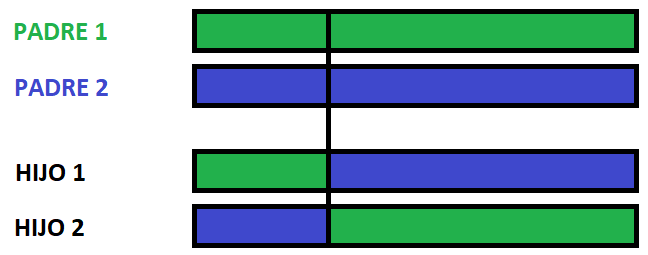
\includegraphics[scale=0.5]{imagenes/Crossover1point.png}
%%         \caption{$y=x$}
%         \label{fig:Crossover1point}
%     \end{subfigure}
%     \hfill
%     \begin{subfigure}[b]{0.3\textwidth}
%         \centering
%         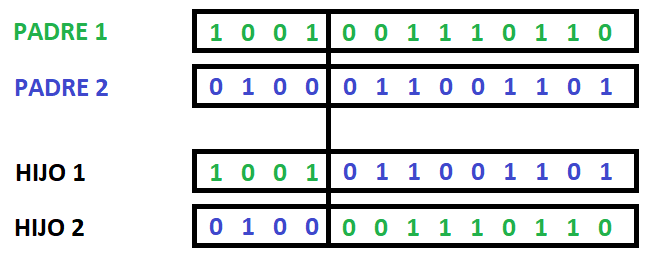
\includegraphics[scale=0.5]{imagenes/Crossover1pointNumber.png}
%%         \caption{$y=3\sin x$}
%         \label{fig:Crossover1pointNumber}
%     \end{subfigure}
		\centering
		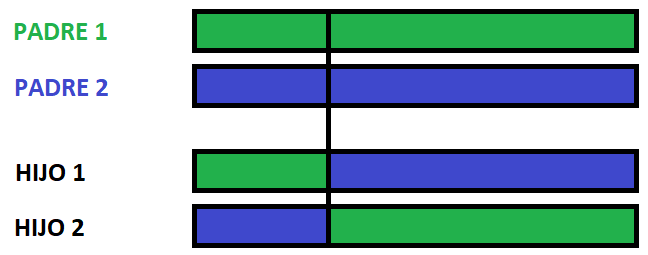
\includegraphics[scale=0.5]{imagenes/Crossover1point.png}
		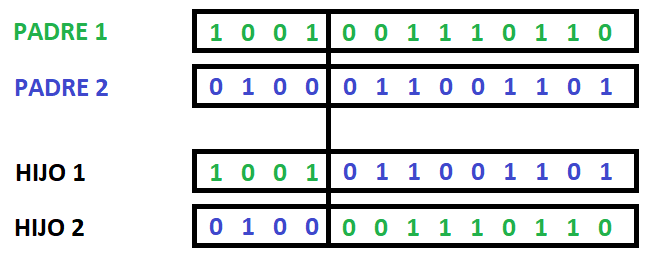
\includegraphics[scale=0.5]{imagenes/Crossover1pointNumber.png}
        \caption{Cruce en un punto}
        \label{fig:Crossover1}
\end{figure}

	\item \textbf{Cruce en dos puntos}: Sigue la misma lógica que el anterior, solo que elegimos dos puntos a partir de los cuales se cambian los elementos de qué padre se asignan a cada hijo. 
Un ejemplo de este tipo de cruce podría ser:
\begin{figure}[H]
		\centering
		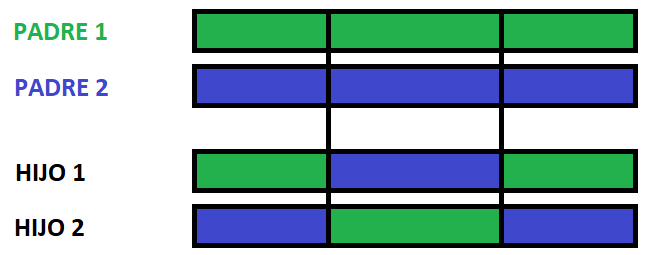
\includegraphics[scale=0.5]{imagenes/Crossover2point.png}
		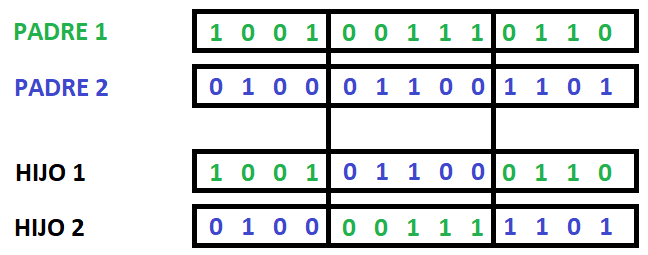
\includegraphics[scale=0.5]{imagenes/Crossover2pointNumber.png}
        \caption{Cruce en dos puntos}
        \label{fig:Crossover2}
\end{figure}
	\item \textbf{Cruce uniforme}: En este caso, en cada cromosoma se elige de forma aleatoria de qué padre lo hereda, cumpliéndose que si un hijo hereda cierto cromosoma de un padre, el otro hijo deberá heredar el mismo cromosoma del otro padre. 
Un ejemplo de este tipo de cruce sería: 
\begin{figure}[H]
		\centering
		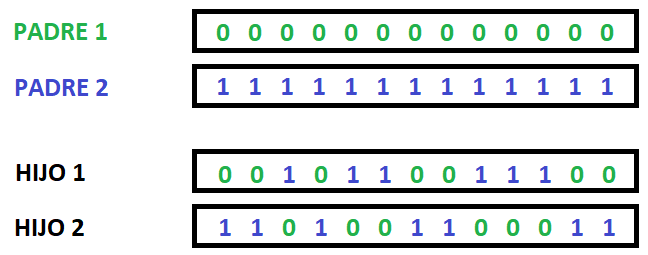
\includegraphics[scale=0.5]{imagenes/CrossoverUniformNumber.png}
        \caption{Cruce Uniforme}
        \label{fig:CrossoverUniform}
\end{figure}
\end{itemize}

El cruce de dos soluciones buenas no tiene por qué siempre dar lugar a una solución mejor o igual de buena. 
Sin embargo, si los padres son buenas soluciones, la probabilidad de tener un hijo bueno es elevada; en el caso de que el hijo no sea una buena solución, será eliminado durante el periodo de reemplazo. 

En nuestro problema es posible que el cruce de dos soluciones no de lugar a una solución factible. 
Esto se debe a la elección aleatoria de qué cromosomas elegir, no estamos teniendo en cuenta el peso que se está alcanzando al asignar cada elemento; por lo que es totalmente posible que  al asignar los elementos a cada hijo se sobrepase la capacidad máxima, dejando por ello de ser una solución factible. 

%Más adelante en este capítulo explicaremos otro tipo de cruce, que es el cruce HUX. 

En nuestro caso, realmente utilizamos una mezcla de cruce en un punto y cruce uniforme. 
Esto es, vamos a asignarle a cada hijo la mitad de cada uno de los padres, pero esta asignación será aleatoria: desordenamos el orden de los índices y lo partimos por la mitad. 
Esto viene representado en el pseudocódigo \ref{alg:CU}.

\begin{algorithm}
\caption{Cruce Uniforme}\label{alg:CU}
\begin{algorithmic}[1]
\Procedure \texttt{Cruce Uniforme}($padre_1, padre_2$)
\State Desordenar los índices que indican la posición de cada elemento
\For{i in 0..$n$}
	\If{i < $n/2$}
		\State \texttt{hijo$_1$[indice[i]]} = \texttt{padre$_1$[indice[i]]}
		\State \texttt{hijo$_2$[indice[i]]} = \texttt{padre$_2$[indice[i]]}
	\Else
		\State \texttt{hijo$_1$[indice[i]]} = \texttt{padre$_2$[indice[i]]}
		\State \texttt{hijo$_2$[indice[i]]} = \texttt{padre$_1$[indice[i]]}
	\EndIf
\EndFor
\EndProcedure
\end{algorithmic}
\end{algorithm}

\subsubsection{Mutación}

Los primeros intentos de mezclar computación y evolución no progresaron porque pusieron énfasis en los textos de biología del momento y confiaban más en la mutación que en el cruce para generar nuevas combinaciones de genes. 

La mutación consiste en modificar al azar una muy pequeña parte del cromosoma de los individuos, y permite alcanzar zonas del espacio de búsqueda que no estaban cubiertas por los individuos de la población actual. 
La mutación sola de por sí generalmente no permite avanzar en la búsqueda de una solución, pero nos garantiza que la población no va a evolucionar hacia una población uniforme que no sea capaz de seguir evolucionando. 

De forma similar a lo explicado en el Operador de Reparación, una vez que obtengamos la nueva solución debemos comprobar si podemos introducir más elementos, con el fin de maximizar el valor que puede llegar a tener. 
Esto también lo haremos siguiendo la misma lógica: ir introduciendo los genes con mayor proporción $valor\_acumulado/peso$. 

El pseudocódigo de nuestra implementación de la mutación viene expresada en Algoritmo \ref{alg:Mutation}. 

\begin{algorithm}
\caption{Mutación}\label{alg:Mutation}
\begin{algorithmic}[1]
\Procedure \texttt{Mutación}($poblacion$, $prob\_mut$)
\State Calcular el número de cromosomas que mutarán $\xrightarrow{}{}$ \texttt{nmut = $n$*prob\_mut}
\State Almacenar de forma aleatoria sin repetición \texttt{nmut} cromosomas de \texttt{poblacion} $\xrightarrow{}{}$\texttt{mutacion}
\For{i in 0..\texttt{nmut}}
	\State Elegir dos genes con distinto valor de forma aleatoria
	\If{Al intercambiar los genes sigue siendo válido}
		\State Intercambiar los genes
	\Else
		\State Volver al paso anterior
	\EndIf
	\State \texttt{anadido = true} 
	\While{\texttt{anadido}}
		\State \texttt{anadido} = Añadir elemento usando Greedy
	\EndWhile
	\State Calcular el valor de la función \textit{fitness}
\EndFor
\EndProcedure
\end{algorithmic}
\end{algorithm}

\subsubsection{Operador de Reemplazo Estacionario}

Una vez que hemos generado nuevas soluciones a partir del cruce de soluciones de la población existente, es necesario establecer un criterio sobre qué soluciones se mantienen o insertan en la población para la siguiente generación. 
En esta versión del Operador de Reemplazo el criterio que se sigue es el enfrentamiento de al población actual con las soluciones hijas, la población resultante estará compuesta de aquellos con mayor valor al calcular su función \textit{fitness}. 

En concreto, para lo que se aplica en el algoritmo base, AG, tenemos en cuenta que solo generamos 2 soluciones hijas antes de enfrentarlas con la población. 
Por ello, se ha optado por un método simplificado de enfrentamiento que consiste en encontrar cuáles son las 2 peores soluciones de la población actual (es decir, aquellas soluciones de la población actual con menor valor \textit{fitness}) y comprobar si las hijas son mejores o no. 
Se puede seguir su esquema en el pseudocódigo \ref{alg:ORE}. 
Usaremos los índices de forma que indique un orden de valores \textit{fitness}, por ejemplo, dados \texttt{padre$_1$} y  \texttt{padre$_2$}, se cumplirá que \textit{fitness}(\texttt{padre$_1$}) > \textit{fitness}(\texttt{padre$_2$}). 
Además, por conveniencia en la notación, se entenderá que \texttt{solucion$_i$} > \texttt{solucion$_j$} significa que el valor \textit{fitness} de \texttt{solucion$_i$} es mayor al de \texttt{solucion$_j$}.

Más adelante en la sección de ``Componentes de CHC'' de este capítulo se presenta la versión más generalizada de este tipo de enfrentamiento.

\begin{algorithm}
\caption{Operador de Reemplazo Estacionario}\label{alg:ORE}
\begin{algorithmic}[1]
\Procedure \texttt{Op Reemplazo Estacionario}
\State Calcular los 2 peores padres de la población actual $\xrightarrow{}{}$ \texttt{padre$_1$}, \texttt{padre$_2$}.
\If{\texttt{hijo$_1$} > \texttt{padre$_1$} \&\& \texttt{hijo$_2$} > \texttt{padre$_2$}}
	\State Intercambiar ambas soluciones de la población por ambos hijos
\ElsIf{\texttt{hijo$_1$} > \texttt{padre$_2$}}
	\State Intercambiar la peor solución de la población por el mejor hijo
\Else
	\State No hacer nada, ya que los dos hijos son peores que las peores soluciones de la población
\EndIf
\EndProcedure
\end{algorithmic}
\end{algorithm}

\section{CHC}

El algoritmo CHC utiliza un método de selección elitista que, combinada con un mecanismo de prevención de incesto y un método para obligar que la población diverja cada vez que converge, permite el mantenimiento de la diversidad de la población. 
Este algoritmo se ha utilizado de forma exitosa en el pasado para problemas de optimización estáticos. 

El algoritmo CHC (\textit{Cross-generational elitist selecition, Heterogeneous recombination and Cataclysmic mutation}) propuesto por Eshelman utiliza un método de selección elitista  combinado con un cruce altamente disruptivo para promover la diversidad de la población. 
La principal característica de este algoritmo es su capacidad de prevenir la convergencia de la población, algo que, como luego comprobaremos, será útil en nuestro problema. 

%En este algoritmo no se necesita de la mutación como era necesario en el AG, esto se debe precisamente a su característica principal, es capaz de forzar la diversidad de la población, por lo que la mutación deja de ser necesaria.

Originalmente, cuando la población converge se pueden tomar dos acciones:
\begin{itemize}
	\item Reiniciar la población entera de forma aleatoria con excepción de la mejor solución
	\item Reiniciar la población utilizando la mejor solución como base y generando el resto realizando modificaciones sobre esta.
\end{itemize}
Sin embargo, esto es solo útil cuando se tienen bastantes evaluaciones. 
En nuestro problema realizar esto resultaría en una pérdida de tiempo e iteraciones importantes, por lo tanto, no se tendrá en cuenta. 

\subsection{Pseudocódigo}

\begin{algorithm}
\caption{Algoritmo CHC}\label{alg:CHC}
\begin{algorithmic}[1]
\Procedure \texttt{AG}($EMax > 0, nelem > 0$)
\State Generar una población inicial aleatoria
\State Calcular la función \textit{fitness} de cada individuo
\State \texttt{generacion} = 0
\State \texttt{threshold} = $n$/4
\While{\texttt{generacion} < EMax}
	\State Calcular el número de parejas a formar para el cruce $\xrightarrow{}{} ncruce = pcruce*nelem$
	\State Desordenar los elementos de la población actual y comprobar si cumplen la condición de prevención de incesto (distancia de Hamming > \texttt{threshold}) de dos en dos
	\If{\texttt{hamming} > \texttt{threshold}}
		\State Almacenar las soluciones $\xrightarrow{}{}$ \texttt{parejas}
	\EndIf
	\If{\texttt{parejas} = $\emptyset$}
		\If{\texttt{threshold} $\neq$ 0}
			\State \texttt{threshold} = \texttt{threshold}-1
		\EndIf
	\Else
		\For{i$\in [0,\texttt{parejas.size()}]$; i=i+2}
			\State Generar 2 hijos cruzando \texttt{parejas}$[i]$ y \texttt{parejas}$[i+1]$
			\State Aplicar el Operador de Reparación sobre ambos hijos
			\State Calcular la función \textit{fitness} de cada hijo
			\State Almacenar dichos hijos $\xrightarrow{}{}$ \texttt{hijos}
		\EndFor
		\State Aplicar el Operador de Selección sobre la población actual e \texttt{hijos}
	\EndIf
	\State \texttt{generacion} = \texttt{generacion}+1
\EndWhile
\EndProcedure
\end{algorithmic}
\end{algorithm}

\subsection{Componentes}
\subsubsection{Operador de reparación}
Se utilizará el mismo que se ha presentado anteriormente en los componentes de AG. 
Véase el pseudocódigo \ref{alg:OR}.

\subsubsection{Cruce HUX}

El cruce HUX (\textit{Half Uniform Crossover}) se caracteriza por, dados dos cromosomas, asignarle a los resultados del cruce en primer lugar los genes comunes a ambos padres y el resto de los genes serán repartidos a partes iguales entre ambos padres. 
Es decir, exactamente la mitad de los genes no coincidentes se intercambian en los hijos. 

A continuación se detallará en forma de pseudocódigo (\ref{alg:HUX}) el comportamiento de este tipo de cruce. 
Aunque primero se mostrará un ejemplo de este tipo de cruce en Figura \ref{fig:HUX}.

\begin{figure}
		\centering
		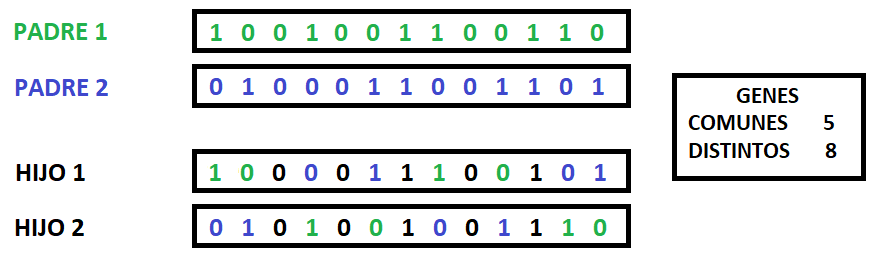
\includegraphics[scale=0.5]{imagenes/CrossoverHUX.png}
        \caption{Cruce HUX}
        \label{fig:HUX}
\end{figure}

\begin{algorithm}
\caption{Cruce HUX}\label{alg:HUX}
\begin{algorithmic}[1]
\Procedure \texttt{Cruce HUX}($padre_1, padre_2$)
\State Asignar los genes comunes de los padres a ambos hijos
\State Desordenar los índices que indican la posición de cada gen restante $\xrightarrow{}{}$ Supongamos tamaño $m \leq n$
\For{i in 0..$m$}
	\If{i < $m/2$}
		\State \texttt{hijo$_1$[indice[i]]} = \texttt{padre$_1$[indice[i]]}
		\State \texttt{hijo$_2$[indice[i]]} = \texttt{padre$_2$[indice[i]]}
	\Else
		\State \texttt{hijo$_1$[indice[i]]} = \texttt{padre$_2$[indice[i]]}
		\State \texttt{hijo$_2$[indice[i]]} = \texttt{padre$_1$[indice[i]]}
	\EndIf
\EndFor
\EndProcedure
\end{algorithmic}
\end{algorithm}

\subsubsection{Reemplazo Elitista}

Es una generalización del Operador de Reemplazo Estacionario del AG (Algoritmo \ref{alg:ORE}). 
En este caso tenemos que enfrentar toda la población de hijos (con tamaño menor igual al tamaño de la población) contra toda la generación anterior. 
Por ello, no podemos seguir el método de obtener los $x$ peores elementos de la población para enfrentarlos con los hijos; así que optaremos por otro razonamiento. 

Se ha optado por, a grandes rasgos, juntar ambas poblaciones (generación actual y descendientes) en una sola y ordenarlas en base a su valor \textit{fitness}. 
De esta forma, al final	tenemos todas nuestras soluciones ordenadas de mejor a peor y solo tenemos que quedarnos con las $n$ para formar la nueva población. 

Este comportamiento se puede ver reflejado en su pseudocódigo (Algoritmo \ref{alg:Enfrentamiento})

\begin{algorithm}[H]
\caption{Enfrentamiento CHC}\label{alg:Enfrentamiento}
\begin{algorithmic}[1]
\Procedure \texttt{Enfrentamiento}($poblacion, hijos$)
\State Calcular la función \textit{fitness} de \texttt{poblacion} e \texttt{hijos}
\State Unir ambas poblaciones $\xrightarrow{}{}$ \texttt{pobTotal}
\State Unir los valores de ambas poblaciones $\xrightarrow{}{}$ \texttt{valorTotal} 
\State Ordenar los elementos de \texttt{pobTotal} según \texttt{valorTotal} (orden descendente)
\State Asignar a la población actual los $n$ primeros elementos de \texttt{pobTotal}
\EndProcedure
\end{algorithmic}
\end{algorithm}

%
\chapter{Componentes de la propuesta}

En este capítulo se presentan los distintos componentes que se han ido desarrollando como modificaciones de los distintos componentes de los algoritmos de referencia. 
Es importante mencionar que en este capítulo no solo se harán mención de aquellas modificaciones que han resultado fructuosas, si no también aquellas que no han mejorado los resultados de versiones anteriores. 
Estas últimas se conformarán su propia sección aparte al final del capítulo. 
Se describirán detalladamente además de usar pseudocódigo para representarlos.

Téngase en cuenta que solo se explicará brevemente el por qué de estas modificaciones, ya que entraremos en este tema en más profundidad en el siguiente capítulo. 

\section{Histórico}

Al tener tan pocas evaluaciones y con un tamaño tan pequeño de la población no podemos permitirnos una exploración del vecindario de las distintas soluciones en direcciones que en el momento se podrían considerar erróneas, es decir, que ocasionarían que empeorasen las soluciones. 
Por ello, se plantea un sistema capaz de ``recordar'' buenos elementos y malos elementos de la solución; considerándose ``buenos elementos'' aquellos que aparecen en gran medida en las mejores soluciones y no se encuentran en las peores, y ``malos elementos'' aquellos que aparecen en gran medida en las peores soluciones y no se encuentran en las mejores. 
A esto lo llamaremos \textbf{histórico}. 

De esta forma, podemos guiar la exploración de vecindario hacia aquellos elementos que han demostrado ser ``buenos'' y alejarlos de aquellos que han demostrado ser ``malos''. 
Esta lógica la podemos aplicar en el Operador de Reparación y/o en la Mutación. 
Esto se haría sustituyendo la lógica Greedy de tener en cuenta el ratio $valor\_acumulado/peso$ a la hora de añadir o eliminar elementos por un fomento del uso de los datos del histórico: se intentarán añadir de forma aleatoria entre los mejores elementos y se intentarán eliminar de forma aleatoria entre los peores elementos. 

Sin embargo, no podemos permitir que esto guíe toda la ejecución, tenemos que decidir un par de cosas:
\begin{itemize}
	\item ¿Cuándo se para de recopilar datos para generar el histórico? 
	Si recopilamos información de pocas iteraciones puede ocasionar que los datos obtenidos no sean representativos, ya que es posible que no se hayan alcanzado en el momento suficientes soluciones buenas. 
	Si recopilamos información de demasiadas iteraciones puede suponer que los datos obtenidos no sean representativos, ya que la población hubiese podido converger por lo que no hay ningún elemento que se pudiese considerar ``bueno'' o ``malo''; además de que si se dejan pocas ejecuciones para el uso del histórico no se va a poder alcanzar mucha mejora. 
	\item ¿Durante cuántas ejecuciones deberíamos utilizar el histórico? 
	En otras palabras, ¿una vez obtenido los datos del histórico deberíamos utilizarlos hasta el final del algoritmo? 
	La respuesta a esto es: no se debería. 
	Esto es porque no podemos esperar que los datos obtenidos mediante el histórico sean del todo fiables, es decir, podrían estar guiando la solución hasta un máximo local, por lo que las soluciones de la población convergerían rápidamente. 
\end{itemize}

Por lo tanto, llegamos a la conclusión de que no podemos utilizar únicamente el histórico. 
Por ello, lo que haremos será intercalar varias etapas de recopilación de datos y uso del histórico generado. 
Durante la recopilación de datos se procederá de la misma forma que lo haría si esta modificación no estuviese añadida, con la excepción de que se irá guardando en un archivo las distintas soluciones que estamos alcanzando para luego hacer el estudio de sus elementos. 
Cada etapa tiene una duración de 50 iteraciones seguidas, con lo que se tendría que cada uso individual del histórico estaría compuesto de 100 iteraciones (50 iteraciones de recopilación de datos y 50 iteraciones de uso de dichos datos). 
De esta forma, repetimos este proceso 4 veces y las 50 iteraciones restantes se dedicarán al comportamiento usual del algoritmo (por simplicidad a la hora de implementar el código, esto es equivalente a la repetición de una etapa de recopilación de datos). 
Este esquema se ve representado de forma genérica, por simplicidad, en Algoritmo \ref{alg:Historico_Estructura}.

\begin{algorithm}[H]
\caption{Estructura General del Histórico}\label{alg:Historico_Estructura}
\begin{algorithmic}[1]
\Procedure \texttt{Histórico}
\State \texttt{RecDatos} = \texttt{True}
\For{\texttt{i = 0; i < NEVALUACIONES; ++i}}
	\If{\texttt{i}\%50==0 \&\& \texttt{i}$\neq$ 0} /* Puntos de cambio */
		\If{i\%100} /* Empezamos a recopilar datos */
			\State \texttt{RecDatos = True}
			\State Eliminar todos los datos actuales del histograma
			\State Recopilar las soluciones de la población actual
		\Else
			\State \texttt{RecDatos = False}
		\EndIf
	\EndIf
	\If{\texttt{RecDatos}}
		\State Ejecutar los componentes de la manera original
		\State Recopilar las nuevas soluciones
	\Else 
		\State Ejecutar los componentes usando los datos del histórico
	\EndIf
\EndFor
\EndProcedure
\end{algorithmic}
\end{algorithm}

Las modificaciones realizadas al Operador de Reparación y a la Mutación se verán representadas respectivamente en Algoritmo \ref{alg:Historico_OR} y Algoritmo \ref{alg:Historico_Mutacion}. 
Para el pseudocódigo \ref{alg:Historico_Mutacion} téngase en cuenta la siguiente notación:
\begin{itemize}
	\item \texttt{Mejores}: Aquellos elementos que suelen estar presentes en las mejores soluciones, pero no en las peores.
	\item \texttt{Peores}: Aquellos elementos que suelen estar presentes en las peores soluciones, pero no en las mejores. 
	\item \texttt{Sin información}: Aquellos elementos que frecuentemente no aparecen en las mejores ni en las peores soluciones o que aparecen en ambas (por lo que no nos aporta ninguna información ya que no se puede considerar un elemento determinista en lo buena que es una solución).
\end{itemize}

\begin{algorithm}
\caption{Histórico en Operador de Reparación}\label{alg:Historico_OR}
\begin{algorithmic}[1]
\Procedure \texttt{Historico\_OR}($hijo$)
\State Calcular el peso total de \texttt{hijo} $\xrightarrow{}{}$ \texttt{pesoHijo}
\If{\texttt{pesoHijo > c}}
	\State Eliminar de forma aleatoria los peores elementos según el histórico hasta que \texttt{pesoHijo} deje de sobrepasar \texttt{c}
	\State Si no es posible lo anterior y sigue dándose la condición, eliminar de forma aleatoria los elementos que no aparecen en el histórico hasta que \texttt{pesoHijo} deje de sobrepasar \texttt{c}
	\State Si no es posible lo anterior y sigue dándose la condición, eliminar de forma aleatoria los mejores elementos según el histórico hasta que \texttt{pesoHijo} deje de sobrepasar \texttt{c}
\Else
	\State Añadir de forma aleatoria los mejores elementos según el histórico sin que \texttt{pesoHijo} sobrepase \texttt{c}
	\State Añadir de forma aleatoria los elementos que no aparecen en el histórico sin que \texttt{pesoHijo} sobrepase \texttt{c}
	\State Añadir de forma aleatoria los peores	elementos según el histórico sin que \texttt{pesoHijo} sobrepase \texttt{c}
\EndIf
\EndProcedure
\end{algorithmic}
\end{algorithm}

\begin{algorithm}
\caption{Histórico en Mutación}\label{alg:Historico_Mutacion}
\begin{algorithmic}[1]
\Procedure \texttt{Historico\_Mutacion}($solucion$)
\State \texttt{sustituido = False}
%\State /*Se establece una lista de prioridades sobre qué par de elementos mutar (uno se elimina y otro se añade)*/
%\State /*Por comodidad y simplicidad se considerará que cada uno de los siguientes enunciados se comporta como una comprobación sobre si se puede realizar dicho cambio
%\State /* - en caso positivo, lo realiza y establece \texttt{sustituido = True} y no comprueba el resto*/
%\State /* - en caso negativo, pasa al siguiente enunciado*/
%\State /*Para no añadir excesivo texto que pudiese hacer que los enunciados se entendiesen menos, todos los enunciados tienen la forma 'Sustituir \texttt{x} elemento existente en la solución por \texttt{y} elemento no existente en la solución' $\xrightarrow{}{}$ 'Sustituir \texttt{x} por \texttt{y}' */
\If{\texttt{!sustituido} \&\& Se puede sustituir un \texttt{peor} elemento por un \texttt{mejor} elemento}
	\State Sustituir \texttt{peor} por \texttt{mejor}
	\State \texttt{sustituido} $\leftarrow{}{}$ \texttt{true}
\ElsIf{\texttt{!sustituido} \&\& Se puede sustituir un \texttt{sin información} elemento por un \texttt{mejor} elemento}
	\State Sustituir \texttt{sin información} por \texttt{mejores}
	\State \texttt{sustituido} $\leftarrow{}{}$ \texttt{true}	
	
\ElsIf{\texttt{!sustituido} \&\& Se puede sustituir un \texttt{peor} elemento por un \texttt{sin información} elemento}
	\State Sustituir \texttt{peores} por \texttt{sin información}
	\State \texttt{sustituido} $\leftarrow{}{}$ \texttt{true}

\ElsIf{\texttt{!sustituido} \&\& Se puede sustituir un \texttt{sin información} elemento por un \texttt{sin información} elemento}	
	\State Sustituir \texttt{sin información} por \texttt{sin información}
	\State \texttt{sustituido} $\leftarrow{}{}$ \texttt{true}
	
\ElsIf{\texttt{!sustituido} \&\& Se puede sustituir un \texttt{mejores} elemento por un \texttt{mejores} elemento}	
	\State Sustituir \texttt{mejores} por \texttt{mejores}
	\State \texttt{sustituido} $\leftarrow{}{}$ \texttt{true}

\ElsIf{\texttt{!sustituido} \&\& Se puede sustituir un \texttt{peores} elemento por un \texttt{peores} elemento}		
	\State Sustituir \texttt{peores} por \texttt{peores}
	\State \texttt{sustituido} $\leftarrow{}{}$ \texttt{true}

\ElsIf{\texttt{!sustituido} \&\& Se puede sustituir un \texttt{mejores} elemento por un \texttt{sin información} elemento}		
	\State Sustituir \texttt{mejores} por \texttt{sin información}
	\State \texttt{sustituido} $\leftarrow{}{}$ \texttt{true}

\ElsIf{\texttt{!sustituido} \&\& Se puede sustituir un \texttt{sin información} elemento por un \texttt{peores} elemento}	
	\State Sustituir \texttt{sin información} por \texttt{peores}
	\State \texttt{sustituido} $\leftarrow{}{}$ \texttt{true}

\ElsIf{\texttt{!sustituido} \&\& Se puede sustituir un \texttt{mejores} elemento por un \texttt{peores} elemento}		
	\State Sustituir \texttt{mejores} por \texttt{peores}
	\State \texttt{sustituido} $\leftarrow{}{}$ \texttt{true}
	
\EndIf
\State Aplicar Operador de Reparación con Histórico para rellenar más las soluciones
\EndProcedure
\end{algorithmic}
\end{algorithm}

\section{GRASP}

En el capítulo 6 se ha explicado por qué seguimos un enfoque \textit{Greedy} en el Operador de Reparación. 
Sin embargo esto tiene un problema, y esto es que es bastante probable que siempre se estén eligiendo los mismos pocos elementos cada vez que se usa este componente. 
Si realmente ocurre eso, ocasionaría que la población converja y la evolución se estanque; por ello, debemos encargarnos de encontrar otra alternativa con la que podamos aumentar la diversidad de la población. 

Sin embargo, la diversidad en la población es un arma de doble filo. 
La diversidad es necesaria para explorar el espacio de soluciones, pero puede causar que no finalice el proceso de exploración. 
Si este es el caso, entonces no se le dedicará suficiente tiempo a la fase de explotación, que es esencial para obtener soluciones de mejor calidad. 
Por lo tanto, utilizaremos un operador capaz de introducir cierta diversidad a la población a la vez que asegura cierta calidad. 
Esto es, utilizaremos el operador GRASP (\textit{Greedy Randomized Adaptive Search Procedure}) \parencite{herrera-poyatosGeneticMemeticAlgorithm2017}. 

El GRASP vendrá presentado en Algoritmo \ref{alg:GRASP}. 
De forma simplificada, GRASP utiliza de base el algoritmo Greedy para obtener cierta cantidad de mejores elementos, eligirá aleatoriamente uno de ellos y lo devolverá. 
Lo que se entiende como ``mejor elemento'' para GRASP es lo mismo que para lo que se propuso durante la justificación del operador Greedy. 
Además, la cantidad de elementos a considerar dependerá del valor aportado por el mejor elemento; en concreto, solo se considerarán los elementos cuyo valor relativo ($valor\_acumulado/peso$) varíe en un 10\% del valor acumulado del mejor elemento, es decir:
\begin{itemize}
	\item Si se necesitan añadir elementos, nos quedaremos con los elementos que tengan un valor relativo mayor que $0.9*valor\_relativo\_mayor$.
	\item Si se necesitan eliminar elementos, nos quedaremos con los elementos que tengan un valor relativo menor que $1.1*valor\_relativo\_menor$.
\end{itemize}

\begin{algorithm}
\caption{Operador GRASP}\label{alg:GRASP}
\begin{algorithmic}[1]
\Procedure \texttt{GRASP}($solucion, min$)
\If{\texttt{min}}
	\State Almacenar en \texttt{indices} los elementos activados en \texttt{solucion}
\Else
	\State Almacenar en \texttt{indices} los elementos desactivados en \texttt{solucion}
\EndIf
\State Calcular el valor relativo de \texttt{indices} $\xrightarrow{}{}$ \texttt{valores}
\State \texttt{encontrado = false}
\If{\texttt{min}}
	\State Ordenar \texttt{indices} según \texttt{valores} en orden ascendente
	\For{$i\in 1..size(\texttt{indices}) \&\& !\texttt{encontrado}$}
		\If{\texttt{valores}$_i$ > 1.1$\cdot$\texttt{valores}$_0$}
			\State \texttt{encontrado = true}
			\State Eliminar los elementos de \texttt{indices} desde $i$ hasta $size(\texttt{indices})$
		\EndIf
	\EndFor
\Else
	\State Ordenar \texttt{indices} según \texttt{valores} en orden descendente
	\For{$i\in 1..size(\texttt{indices}) \&\& !\texttt{encontrado}$}
		\If{\texttt{valores}$_i$ < 0.9$\cdot$\texttt{valores}$_0$}
			\State \texttt{encontrado = true}
			\State Eliminar los elementos de \texttt{indices} desde $i$ hasta $size(\texttt{indices})$
		\EndIf
	\EndFor
\EndIf
\State Elegir aleatoriamente algún elemento de \texttt{indices}
\EndProcedure
\end{algorithmic}
\end{algorithm}

\section{Cruce Intensivo}

Para aumentar la explotación de buenas soluciones se propone hacer una modificación en el cruce que realizamos. 
En vez de utilizar el cruce uniforme, que hemos establecido que a cada hijo se le asigna la mitad de los genes de cada uno de los padres (aunque sea de forma aleatoria), en este caso se le asignará un mayor porcentaje de genes del mejor de los padres. 

Para ello, lógicamente tendremos que calcular cuál de los padres es la mejor solución (tiene mayor valor). 
En este caso, no nos sirve aleatorizar una sola lista de índices, ya que la separación no va a ser igualitaria. 
Por lo que tendremos que hacer las separaciones de genes para ambos hijos. 
Una vez hecho esto, se procede de igual forma que en los anteriores cruces, es decir, se le asigna a cada hijo los genes de los padres correspondientes y, posteriormente, se le aplica el operado de reparación a ambos hijos. 
Estoy viene representado en Algoritmo \ref{alg:CI}. 

Por conveniencia, vamos a volver a utilizar la notación que implica que \texttt{padre$_1$} tiene un valor más elevado que \texttt{padre$_2$}.

\begin{algorithm}
\caption{Cruce Intensivo}\label{alg:CI}
\begin{algorithmic}[1]
\Procedure \texttt{Cruce Intensivo}($padre_1, padre_2, porcentaje$)
\State Desordenar los índices (\texttt{indices$_1$}, \texttt{indices$_2$}) que indican la posición de cada elemento
\State \texttt{nelem = $n$*porcentaje}
\For{i in 0..$n$}
	\If{\texttt{i < nelem}}
		\State \texttt{hijo$_1$[indice$_1$[i]]} = \texttt{padre$_1$[indice$_1$[i]]}
		\State \texttt{hijo$_2$[indice$_2$[i]]} = \texttt{padre$_1$[indice$_2$[i]]}
	\Else
		\State \texttt{hijo$_1$[indice$_1$[i]]} = \texttt{padre$_2$[indice$_1$[i]]}
		\State \texttt{hijo$_2$[indice$_2$[i]]} = \texttt{padre$_2$[indice$_2$[i]]}
	\EndIf
\EndFor
\EndProcedure
\end{algorithmic}
\end{algorithm}


\section{Diversidad en la Población Inicial}

Uno de los mayores problemas que se puede tener cuando la población es pequeña y no nos podemos permitir muchas ejecuciones es la falta de diversidad en dicha población. 
Si todos los elementos son muy parecidos entre sí resultará muy difícil llevar a cabo una correcta exploración del espacio de soluciones, ya que las soluciones generadas en el cruce se seguirán pareciendo a sus padres (por lo que serán similares al resto de la población) y en la mutación, al solo intercambiar un par de elementos no se va a conseguir una solución lo suficientemente distinta del resto. 

Por ello, lo primero que debemos garantizar antes de empezar el algoritmo es que tenemos una población inicial lo suficientemente diversa sobre la que trabajar. 
Esto viene representando en el pseudocódigo \ref{alg:PD}. 
Una población inicial diversa se consigue generando las soluciones de forma aleatoria sucesivamente a la vez que se comprueba su similitud (su distancia de Hamming) con respecto al resto de soluciones que ya forman parte de la población. 
Si dicha nueva solución no supera un umbral de diferencias (normalmente representado como un porcentaje del número de elementos totales del problema) con respecto a todas las soluciones introducidas, se descarta esta solución y se vuelve a generar otra. 
Este proceso se repite hasta haber alcanzado el tamaño de población necesario para empezar la ejecución del algoritmo.

\begin{algorithm}
\caption{Población Inicial Diversa}\label{alg:PD}
\begin{algorithmic}[1]
\Procedure \texttt{Población Diversa}($p_\delta$)
\State \texttt{distMin} $\xleftarrow{}{} n\cdot p_\delta$
\State \texttt{npob} $\xleftarrow{}{}$ \texttt{0}
\State \texttt{poblacion} $\xleftarrow{}{} \emptyset$
\While{\texttt{npob}$<$\texttt{numcro}}
	\State Generamos una solución aleatoria $\xrightarrow{}{}$ \texttt{solucion}$_{\texttt{npob}}$
	\State \texttt{nuevo} $\xleftarrow{}{}$ \texttt{true}
	\ForEach{\texttt{sol}$\in$\texttt{poblacion}}
		\If{$distHamming($\texttt{solucion}$_{\texttt{npob}},$\texttt{sol}$) < $\texttt{distMin}}
			\State \texttt{nuevo} $\xleftarrow{}{}$ \texttt{false}
		\EndIf
	\EndFor
	\If{\texttt{nuevo}}
		\State Añadir \texttt{solucion}$_{\texttt{npob}}$ a \texttt{poblacion}
		\State \texttt{npob++}
	\EndIf
\EndWhile
\EndProcedure
\end{algorithmic}
\end{algorithm}

Donde recordemos que $n$ es el número de variables del problema y \texttt{numcro} el tamaño de la población con la que trabajaremos. 
$p\_delta$ representa el porcentaje de elementos del número de variables total que deben ser distintos para considerar que la nueva solución es lo suficientemente diferente al resto de soluciones introducidas en la población; por lo que \texttt{distMin} será dicho número mínimo de elementos distintos. 

\section{Operador NAM}

El operador de Emparejamiento Variado Inverso (\textit{Negative Assortative Mating}) o NAM
\parencite{fernandesStudyNonrandomMating2001} está orientado a generar diversidad. 
Esta es una alternativa a cómo se eligen los individuos de la población que se van a cruzar. 
La lógica de este operador es parecida a la prevención de incesto que se propone en el algoritmo CHC, pero sin ser tan restrictiva. 
Se necesita que los padres sean distintos para conseguir que los hijos aporten diversidad a la población si llegan a ser introducidos. 
Una optativa a esto es el operador NAM. 
En este trabajo se utilizará una versión del NAM.

La implementación de este operador viene representado en el Algoritmo \ref{alg:NAM}. 
Lo que se hace en este operador es elegir a una solución utilizando el Torneo Binario propio de los algoritmos genéticos (en el operador original simplemente se elige un individuo de la población de forma aleatoria). 
Para la segunda solución, primero, debemos obtener algunas soluciones de la población distintas a la primera obtenida para el cruce. 
Una vez hecho esto, elegimos como el segundo padre a la solución del segundo grupo más diferente al primer padre; esto es, se calculará la distancia de Hamming entre el primer padre y las soluciones del segundo grupo, y se elegirá como segundo padre aquella solución con mayor distancia de Hamming.

\begin{algorithm}
\caption{Operador NAM}\label{alg:NAM}
\begin{algorithmic}[1]
\Procedure \texttt{Operador NAM}
\State Aplicar \texttt{Torneo Binario} para obtener al primer padre $\xrightarrow{}{}$ \texttt{padre$_1$}
\State Elegir aleatoriamente sin repetición un subconjunto de la población distinta a \texttt{padre$_1$} $\xrightarrow{}{}$ \texttt{indices}.
\State Calcular la distancia de Hamming entre \texttt{padre$_1$} y cada elemento de \texttt{indices}
\State Establecer como \texttt{padre$_2$} la solución de \texttt{indices} con la mayor distancia de Hamming a \texttt{padre$_1$}
\EndProcedure
\end{algorithmic}
\end{algorithm}

\section{Operador Reemplazo: \textit{Crowding} Determinístico}


Otra forma de intentar mantener cierta diversidad en la población es mediante la modificación del Operador de Reemplazo. 
En vez de siempre eliminar las peores soluciones para introducir otras mejores, se sustituirán individuos de la población similares a las nuevas soluciones si estas últimas son mejores. 
Esto da lugar que se permitirá mantener las peores soluciones en la población siempre que estén aportando diversidad a la población.

Este operador \parencite{mahfoudCrowdingPreselectionRevisited1992} viene representado en el Algoritmo \ref{alg:ORC}. 
En definitiva, el objetivo de este operador será comprobar si las nuevas soluciones (hijas) son mejores que las soluciones de la población actual más cercanas a ellas. 
Si las soluciones hijas constituyen una mejora, entonces sustituirán a las soluciones más cercanas en la población. 

\begin{algorithm}
\caption{Operador de Reemplazo por Cercanía}\label{alg:ORC}
\begin{algorithmic}[1]
\Procedure \texttt{Reemplazo Cercanía}
\For{i in 0..\texttt{numHijos}}
	\State Calcular distancia de Hamming de \texttt{hijo$_i$} a todos los elementos de la población
	\State Elegir la solución con la menor distancia de Hamming a \texttt{hijo$_i$} $\xrightarrow{}{}$ \texttt{solucion}
	\If{\texttt{valor$_{solucion}$ < valor$_{hijo_i}$}}
		\State Sustituir \texttt{solucion} por \texttt{hijo$_i$}
	\EndIf
\EndFor
\EndProcedure
\end{algorithmic}
\end{algorithm}

\subsection{Reemplazo intensivo}

En esta versión, adicionalmente a modificar el operador de reemplazo de forma que las nuevas soluciones sustituirán a las más parecidas siempre que las mejoren, se compararán el resto de soluciones similares (tienen una distancia de Hamming menor que determinado umbral). 
La idea de esta versión es aumentar aún más la diversidad mediante la eliminación de soluciones peores parecidas a aquellas que ya tenemos. 

Si se logra introducir la nueva solución en la población se comprobará si hay más soluciones cercanas. 
En caso negativo no se hará nada más al respecto. 
Sin embargo, en caso positivo, nos quedaremos únicamente con la mejor solución entre todas las consideradas (la nueva y las parecidas en la población), eliminando el resto de la población. 
Como el tamaño de la población debe ser constante, estas vacantes serán cubiertas por soluciones totalmente aleatorias que no sean parecidas a la solución que se ha conseguido mantener en la población. 
Este funcionamiento viene representado en \ref{alg:ORCv}.

\begin{algorithm}
\caption{Operador de Reemplazo por Cercanía intensivo}\label{alg:ORCv}
\begin{algorithmic}[1]
\Procedure \texttt{Reemplazo Cercanía}($\delta_H$)
\For{i in 0..\texttt{numHijos}}
	\State Almacenar los individuos de la población tal que su distancia de Hamming a \texttt{hijo$_i$} sea menor que $\delta_H \xrightarrow{}{} $ \texttt{indCercanos}
	\State Calculamos el elemento de \texttt{indCercanos} con mayor valor
	\State El resto de elementos de \texttt{indCercanos} se sustituye por soluciones generadas aleatoriamente
	\While{La solución generada aleatoriamente sea cercana a una existente}
		\State Sustituirla por otra solución generada aleatoriamente
	\EndWhile
\EndFor
\EndProcedure
\end{algorithmic}
\end{algorithm}

%
\chapter{Evolución en la propuesta \color{red}(In progress)\color{black}}

En este capítulo se realizará un análisis completo paso por paso del proceso de desarrollo del algoritmo. 
Se mostrarán distintas tablas y gráficas comparativas y sus interpretaciones con el fin de justificar la motivación de las distintas modificaciones introducidas explicadas en el capítulo anterior.

\section{Diseño Experimental}
\subsection{Criterio de Parada}

Se han elegido las instancias mencionadas anteriormente (\href{http://cedric.cnam.fr/~soutif/QKP/QKP.html}{(QKP) \textit{instances}}) ya que también se proporcionaban algunos resultados de otros algoritmos, por lo que resultaba conveniente a la hora de comprobar si los resultados obtenidos por nuestros algoritmos bases eran competitivos. 
Ya que, en el caso de que no lo fuesen, tendríamos que buscar otros algoritmos base sobre los que trabajar.
Sin embargo, nos encontramos con un problema, esto es, el criterio de parada presentado en estos casos es el tiempo (se ha tomado como referencia los experimentos realizados en \parencite{garcia-martinezStrategicOscillationQuadratic2014}).
Adicionalmente, el tiempo de parada también depende del número de elementos, $n$, de forma que se tiene:
\begin{itemize}
\item Para $n = 100$, se tienen \textbf{5 segundos} de ejecución.
\item Para $n > 100$, en nuestro caso, $n = 200$ y $n = 300$, se tienen \textbf{30 segundos} de ejecución.
\end{itemize}

Como se ha indicado antes, utilizar el tiempo de ejecución como criterio de parada resulta un problema. 
Esto se debe a que no es un criterio de parada fiable, ya que depende de la capacidad de computación de cada ordenador. 
No es comparable la velocidad de los ordenadores actuales con la velocidad de los ordenadores de dentro de 10 años, de la misma no podemos comparar el rendimiento de un ordenador de hace 10 años con respecto a uno actual. 
E incluso dentro de los ordenadores de la misma generación, dependerá de las características propias de cada computador. 
Por lo que se llega a la conclusión de que si se quiere que los resultados obtenidos en este trabajo puedan ser usados como referencia, o incluso si se quiere recrear el trabajo, en un futuro se debe cambiar el criterio de parada a algo portable, a algo que sea independiente de cuándo se produzca el experimento. 
Por ello, se ha decidido cambiar el criterio de parada a un número de iteraciones máximo. 
Este criterio sí es portable, ya que independientemente de qué tipo de computador se utilice para obtener los resultados siempre se van a obtener los mismos resultados utilizando los mismos parámetros.

Primero debemos indicar lo que entenderemos por iteraciones. 
Denotaremos como iteraciones al número de veces que se repite el procedimiento completo un determinado algoritmo, en nuestro caso se va a traducir en lo siguiente: 
\begin{itemize}
	\item Para el algoritmo \textit{Random}, el número iteraciones será el número de veces que generemos una solución de forma aleatoria.
	\item Para los algoritmos genéticos, una iteración puede suponer un número distinto de evaluaciones. 
	En los algoritmos genéticos al número de iteraciones se llama también generaciones.
\end{itemize}

Dicho esto, para elegir el número de iteraciones máximo que se iba a utilizar se tomó como referencia el tiempo establecido anteriormente. 
En tanto se tenía elegir un número de iteraciones como criterio de parada, se decidió estudiar a qué equivalía actualmente el criterio de parada por tiempo establecido. 
Para ello, mediante una variable \texttt{contador}, se ejecutaron todos los archivos con el tiempo como criterio de parada y se mostraba por pantalla el número de iteraciones que se había alcanzado. 
Tras realizar una media de todos estos datos y redondearlo, obtenemos que el nuevo criterio de parada es \textbf{90000 iteraciones} para todos los archivos. 
El que el número de iteraciones máximo no dependa del número de elementos como lo hacía el tiempo de ejecución máximo se puede justificar en tanto que se necesita más tiempo para realizar todos los cálculos si aumenta el número de datos. 

Además, para asegurarnos que realmente ambos criterios de parada eran equivalentes, se ejecutaron todos los archivos usando el algoritmo base con criterio de parada por iteraciones y por tiempo. 
Nótese que no solo se almacenan las soluciones finales, si no que también se almacenan las soluciones intermedias llegado a ciertos porcentajes de la ejecución. 
Tras esto, se compararon ambos resultados y se pudo comprobar que, efectivamente, eran equivalentes. 

Por lo tanto, se puede decir con seguridad que los cambios que apliquemos a un criterio de parada en específico se puede traducir a un cambio en el otro criterio de parada. 
Esto cabe la pena destacarlo ya que, recordemos, el objetivo de este trabajo es crear un algoritmo útil y competitivo para tratar con problemas \textit{expensive}, por lo que queremos obtener buenos resultados en un tiempo muy reducido. 

Para simular de forma eficiente y suficiente esta reducción de tiempo, se propuso el siguiente cambio con respecto al tiempo como criterio de parada:
\begin{itemize}
	\item En vez de ejecutar los archivos con $n=100$ durante 5 segundos, lo reduciremos a 25ms.
	\item En vez de ejecutar los archivos con $n>100$ durante 30 segundos, lo reduciremos a 150ms.
\end{itemize}
Realizamos un cálculo básico para comprobar qué proporción de la ejecución estaremos realizando con estos nuevos tiempos:
\begin{equation*}
\dfrac{25\cdot 100ms}{5\cdot 1000ms} = 0.5
\hspace{1cm}
\dfrac{150\cdot 100ms}{30\cdot 1000ms} = 0.5
\end{equation*}
Por lo tanto, obtenemos que solo utilizaremos el 0.5\% inicial de cada ejecución, lo que podemos traducir en que nuestro nuevo criterio de parada serán \textbf{450 iteraciones}. 

Con el fin de comprobar que esta reducción había sido suficiente y necesaria, se ejecutan de nuevo todos los archivos con el algoritmo base ahora con 450 iteraciones y comparamos los resultados con los obtenidos anteriormente con 90000 iteraciones. 
Podemos ver que, efectivamente, se han obtenido resultados mucho peores. 

Finalmente, ya hemos establecido nuestro criterio de parada escalable y tenemos unos resultados base que utilizar. 
A partir de esto, nuestro objetivo será mejorar estos resultados lo máximo posible.

\subsection{Parámetros}

La ejecución del programa no requiere de la introducción manual de ningún tipo de parámetro. 
Todos los parámetros que se nombren a continuación vienen definidos dentro del código del programa \texttt{main} como constantes globales o que dependen del propio problema. 

En primer lugar, recordemos brevemente los parámetros que utilizaremos y sus valores. 
Estos parámetros no necesitan ser introducidos manualmente al ejecutar el programa, si no que están definidos como constantes en el código:

\begin{itemize}
	\item \texttt{NEVALUACIONESMAX}: Es el número de iteraciones máximas, mantendremos su valor a 450 por lo explicado en el apartado anterior. 
	\item \texttt{NTRIES}: Para eliminar la aleatoriedad que proviene de la ejecución con una determinada semilla u otra, cada algoritmo se ejecutará \texttt{NTRIES} número de veces, haremos la media de sus ejecuciones y este valor será el resultado que se guardará y se comparará posteriormente con el resto. 
	Para que los resultados puedan ser comparados estadísticamente, pero a la vez se mantenga un tiempo de ejecución razonable, estableceremos su valor a 50.
	\item \texttt{INITSEED}: En relación con la constante anterior, es necesario no utilizar siempre la misma semilla de aleatoriedad, ya que eso resultaría en obtener siempre los mismos resultados, por lo que ejecutarlos varias veces sería una pérdida de tiempo. 
	Así pues, tendremos que usar distintas semillas para cada ejecución. 
	Para asegurar que los resultados sean replicables deben definirse todas estas semillas y que se utilice el mismo conjunto de semillas para todos los algoritmos (para que aún dentro de lo que cabe, todos tengan las mismas condiciones de aleatoriedad). 
	Por conveniencia, en vez de definir todas las semillas a mano, estableceremos manualmente una única semilla inicial que se encargará de generar el resto de semillas que son las que realmente se usarán.
	En nuestro caso, se ha elegido el valor 5. 
	\item \texttt{numcro}: Es el tamaño de la población de individuos que vamos a considerar en los algoritmos. 
	En tanto que el objetivo es obtener buenos resultados en pocas iteraciones, no nos podemos permitir tener un tamaño de población excesivamente grande; ya que a mayor población, más evaluaciones deberán realizarse por generación y esto dará lugar a que se realicen muy pocos cambios de generación (lo que se traduce en pocas iteraciones del algoritmo). 
	Tampoco podemos tener un tamaño de población excesivamente pequeño, ya que resulta un inconveniente el trabajar con muy pocos individuos y este problema no es el objetivo de este trabajo. 
	Por lo tanto, estableceremos su valor a 10.
	\item \texttt{probc}: Es la probabilidad de cruce en los AGs. 
	No lo usamos como parámetro propiamente en el código, ya que para los algoritmos de referencia (AGE y CHC) tienen un número de cruces que se tienen que producir establecidos; en el caso de AGE solo se producirá un cruce por generación y para el CHC se intentarán cruzar todos los individuos posibles. 
	\item \texttt{probm}: Es la probabilidad de mutación en los AGs. Recuérdese que para el CHC no se requiere de esta mutación ya que obtiene la diversidad de otros operadores propios. 
	En la literatura se coincide que el valor de este parámetro debe ser uno bastante pequeño, generalmente entre un 1\% y un 10\% de la población. 
	Para asegurarnos que se produzca una mutación por cambio de generación, establecemos su valor a 0.1.
	\item \texttt{EvaluacionMAX}: Es el número de iteraciones/generaciones máximas. 
	Establecemos su valor a 450 por lo ya explicado en el apartado ``Diseño Experimental''.
	\item \texttt{seed}: Como se ha indicado anteriormente, cada ejecución individual de un algoritmo tendrá asociada una semilla para determinar la aleatoriedad de los acontecimientos y que sea replicable. 
	Este valor se tomará de aquellos que hayan sido generados por \texttt{INITSEED}.
\end{itemize}

En definitiva, a modo de resumen, podemos rápidamente visualizar en la Tabla \ref{Resumen} los distintos parámetros con los que trabajaremos, cuáles son sus usos y sus valores.

\begin{table}[H]
\begin{tabular}{|l|l|l|}
\hline
\rowcolor[HTML]{F7EAC7} 
Parámetros                                 & Resumen                                                                                                                                   & Valor                                                                                 \\ \hline
\rowcolor[HTML]{DAE8FC} 
\texttt{NEVALUACIONESMAX} & \begin{tabular}[c]{@{}l@{}}Criterio de parada: Número de\\ Iteraciones Máximas para \\ cada algoritmo\end{tabular}                       & 450                                                                                   \\ \hline
\rowcolor[HTML]{DDFDFF} 
\texttt{NTRIES}           & \begin{tabular}[c]{@{}l@{}}Número de veces que se va a \\ ejecutar el algoritmo por cada\\ archivo\end{tabular}                           & 50                                                                                    \\ \hline
\rowcolor[HTML]{DAE8FC} 
\texttt{INITSEED}         & \begin{tabular}[c]{@{}l@{}}Semilla inicial para poder \\ generar el resto de semillas que\\ utilizaremos para los algoritmos\end{tabular} & 5                                                                                     \\ \hline
\rowcolor[HTML]{DDFDFF} 
\texttt{EvaluacionMAX}    & \begin{tabular}[c]{@{}l@{}}Criterio de parada: Número de\\ Iteraciones Máximas dicho\\ algoritmo\end{tabular}                            & \texttt{NEVALUACIONESMAX}                                           \\ \hline
\rowcolor[HTML]{DAE8FC} 
\texttt{seed}          & \begin{tabular}[c]{@{}l@{}}Semilla de aleatoriedad para\\ determinada ejecución del \\ algoritmo\end{tabular}                             & \begin{tabular}[c]{@{}l@{}}Valor generado aleatoriamente \\ por \texttt{INITSEED}\end{tabular} \\ \hline
\rowcolor[HTML]{DDFDFF} 
\texttt{numcro}             & \begin{tabular}[c]{@{}l@{}}Número de elementos de la\\ población de soluciones\end{tabular}                                               & 10                                                                                    \\ \hline
\rowcolor[HTML]{DAE8FC} 
\texttt{pmut}             & \begin{tabular}[c]{@{}l@{}}Probabilidad de mutación\\ de las soluciones de la población\\ ({[}0,1{]})\end{tabular}                        & 0.1                                                                                   \\ \hline
\rowcolor[HTML]{DDFDFF} 
\texttt{probc}             & \begin{tabular}[c]{@{}l@{}}Probabilidad de cruce\\ de los individuos de la población\end{tabular}                                               & \begin{tabular}[c]{@{}l@{}}- AG: 2 individuos por Torneo\\- CHC: Todos los posibles\\sin repetición\end{tabular}                                                                                    \\ \hline
\end{tabular}
\caption{\label{Resumen}Resumen de parámetros utilizados}
\end{table}

Es importante mencionar que para todas las ejecuciones se han almacenado no solo los resultados finales, sino las mejores soluciones que se han encontrado en diversos momentos de la ejecución (\textit{milestones}). 
Es decir, se han almacenado las mejores soluciones encontradas en los porcentajes de ejecución $\{1,2,3,5,10,20,30,40,50,60,70,80,90,100\}$. 
Esto se podrá ver claramente cuando se muestren gráficas que representen de forma visual el \textit{ranking} de los distintos algoritmos comparados; sin embargo, por falta de espacio en las páginas y comodidad tanto para la autora como para el lector, en las tablas solo se mostrarán los resultados finales de las ejecuciones, aunque se harán menciones al comportamiento general (para determinar si puede estar convergiendo a una solución de forma prematura). 

Tambiés es necesario comentar que los datos tienen distintas escalas, por lo que a la hora de estudiar las diferencias entre los resultados de las \textit{milestones} no podemos simplemente hacer una media de todos los valores. 
Por ello se ha intentado normalizar los intervalos considerando que el resultado final es el máximo del intervalo y 0 el mínimo (ya que en nuestro problema todos los valores de los elementos, individuales y combinados, son no negativos). 
Por tanto, en las tablas de diferencias y sus respectivas gráficas se ven representados los porcentajes de dichos intervalos asociados a las diferencias entre el resultado final y el resultado de cada \textit{milestone}.

Todos los códigos y resultados pueden ser encontrados en el \href{https://github.com/Itrilor/TFG/tree/main}{respositorio de Github de este trabajo}. 

\section{Algoritmos de Referencia experimentación}

\color{red}

Para empezar, debemos mostrar los resultados obtenidos de aplicar los algoritmos de referencia al problema con sus condiciones iniciales, esto es, con 90000 iteraciones en vez de 450. 


Preguntar si ha habido algún progreso con esto

\color{black}

\section{Resultados versión expensive}

Tal y como hemos mencionado en capítulos anteriores, el objetivo de este trabajo es el desarrollo de un algoritmo que ante todo sea capaz de obtener resultados competentes en poco tiempo, lo que se puede traducir en un número pequeño de iteraciones. 
Por lo que el siguiente paso será obtener los resultados para los mismos algoritmos que en la sección anterior, pero para su versión \textit{expensive}, es decir, utilizaremos un número de iteraciones máximas de 450, tal y como hemos establecido en los parámetros. 

Obtener resultados para esta versión es fundamental, ya que nos aporta las bases sobre las que trabajaremos y necesitaremos mejorar todo los posible durante este desarrollo. 
También es interesante observar lo mucho que empeoran los resultados frente a su versión normal, lo cual era de esperar, ya que recordemos que solo estamos utilizando el primer 0.5\% de las iteraciones de su versión original. 

Por ello, en la tabla \ref{AGEU450}, se muestran los resultados de la ejecución del AGE, mientras que en la tabla \ref{CHC450}, se muestran los resultados de la ejecución del CHC. 

Cabe mencionar que originalmente el único algoritmo de referencia que se consideró era el AG. 
Sin embargo, durante el desarrollo se consideró la posibilidad de introducir elementos propios del algoritmo CHC, ya que es un algoritmo bastante balanceado que suele dar buenos resultados. 
Por ello, también se realizó una comparación entre los resultados obtenidos por el AG y los del CHC. 
Esta comparación se puede apreciar en la gráfica \ref{fig:AGEUvsCHC}.

\begin{figure}
     \centering
     \begin{subfigure}[b]{0.45\textwidth}
         \centering
         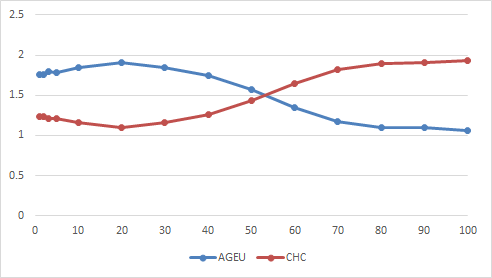
\includegraphics[width=\textwidth]{imagenes/Experimental/AGEUvsCHC.png}
         \caption{Ranking durante todas las \textit{milestones}}
         \label{fig:AGEUvsCHC_lineas}
     \end{subfigure}
     \hfill
     \begin{subfigure}[b]{0.45\textwidth}
         \centering
         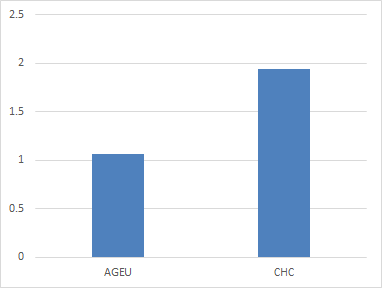
\includegraphics[width=\textwidth]{imagenes/Experimental/barras/AGEUvsCHC.png}
         \caption{Ranking final}
         \label{fig:AGEUvsCHC_barras}
     \end{subfigure}
        \caption{Comparación de AGEU y CHC}
        \label{fig:AGEUvsCHC}
\end{figure}


También podemos apreciar en la tabla \ref{diferenciasAGEU} la media de las distancias entre las soluciones obtenidas en cada \textit{milestone} en la ejecución de AGEU con la final (también más visible en la gráfica \ref{fig:DiferenciasAGEU}). 

%Diferencias AGEU
\begin{table}[]
\begin{tabular}{|cclcclccl|}
\hline
\rowcolor[HTML]{FFFFC7} 
\multicolumn{9}{|c|}{\cellcolor[HTML]{FFFFC7}AGEU   450}                                                                                                                                                                                                                                                                                                                                                                                                                                                                                                 \\ \hline
\rowcolor[HTML]{F7EAC7} 
\multicolumn{1}{|c|}{\cellcolor[HTML]{F7EAC7}n}                               & \multicolumn{1}{c|}{\cellcolor[HTML]{F7EAC7}milestone} & \multicolumn{1}{l|}{\cellcolor[HTML]{F7EAC7}Diferencia} & \multicolumn{1}{c|}{\cellcolor[HTML]{F7EAC7}n}                               & \multicolumn{1}{c|}{\cellcolor[HTML]{F7EAC7}milestone} & \multicolumn{1}{l|}{\cellcolor[HTML]{F7EAC7}Diferencia} & \multicolumn{1}{c|}{\cellcolor[HTML]{F7EAC7}n}                               & \multicolumn{1}{c|}{\cellcolor[HTML]{F7EAC7}milestone} & Diferencia  \\ \hline
\rowcolor[HTML]{DAE8FC} 
\multicolumn{1}{|c|}{\cellcolor[HTML]{FFFFC7}}                                & \multicolumn{1}{c|}{\cellcolor[HTML]{DAE8FC}1}         & \multicolumn{1}{l|}{\cellcolor[HTML]{DAE8FC}20.5989}    & \multicolumn{1}{c|}{\cellcolor[HTML]{FFFFC7}}                                & \multicolumn{1}{c|}{\cellcolor[HTML]{DAE8FC}1}         & \multicolumn{1}{l|}{\cellcolor[HTML]{DAE8FC}27.5017199} & \multicolumn{1}{c|}{\cellcolor[HTML]{FFFFC7}}                                & \multicolumn{1}{c|}{\cellcolor[HTML]{DAE8FC}1}         & 28.8527814  \\ \cline{2-3} \cline{5-6} \cline{8-9} 
\rowcolor[HTML]{DDFDFF} 
\multicolumn{1}{|c|}{\cellcolor[HTML]{FFFFC7}}                                & \multicolumn{1}{c|}{\cellcolor[HTML]{DDFDFF}2}         & \multicolumn{1}{l|}{\cellcolor[HTML]{DDFDFF}16.3468}    & \multicolumn{1}{c|}{\cellcolor[HTML]{FFFFC7}}                                & \multicolumn{1}{c|}{\cellcolor[HTML]{DDFDFF}2}         & \multicolumn{1}{l|}{\cellcolor[HTML]{DDFDFF}22.9143937} & \multicolumn{1}{c|}{\cellcolor[HTML]{FFFFC7}}                                & \multicolumn{1}{c|}{\cellcolor[HTML]{DDFDFF}2}         & 23.90292863 \\ \cline{2-3} \cline{5-6} \cline{8-9} 
\rowcolor[HTML]{DAE8FC} 
\multicolumn{1}{|c|}{\cellcolor[HTML]{FFFFC7}}                                & \multicolumn{1}{c|}{\cellcolor[HTML]{DAE8FC}3}         & \multicolumn{1}{l|}{\cellcolor[HTML]{DAE8FC}14.0108}    & \multicolumn{1}{c|}{\cellcolor[HTML]{FFFFC7}}                                & \multicolumn{1}{c|}{\cellcolor[HTML]{DAE8FC}3}         & \multicolumn{1}{l|}{\cellcolor[HTML]{DAE8FC}20.5848898} & \multicolumn{1}{c|}{\cellcolor[HTML]{FFFFC7}}                                & \multicolumn{1}{c|}{\cellcolor[HTML]{DAE8FC}3}         & 21.25337355 \\ \cline{2-3} \cline{5-6} \cline{8-9} 
\rowcolor[HTML]{DDFDFF} 
\multicolumn{1}{|c|}{\cellcolor[HTML]{FFFFC7}}                                & \multicolumn{1}{c|}{\cellcolor[HTML]{DDFDFF}5}         & \multicolumn{1}{l|}{\cellcolor[HTML]{DDFDFF}10.5074}    & \multicolumn{1}{c|}{\cellcolor[HTML]{FFFFC7}}                                & \multicolumn{1}{c|}{\cellcolor[HTML]{DDFDFF}5}         & \multicolumn{1}{l|}{\cellcolor[HTML]{DDFDFF}16.5204328} & \multicolumn{1}{c|}{\cellcolor[HTML]{FFFFC7}}                                & \multicolumn{1}{c|}{\cellcolor[HTML]{DDFDFF}5}         & 17.2023095  \\ \cline{2-3} \cline{5-6} \cline{8-9} 
\rowcolor[HTML]{DAE8FC} 
\multicolumn{1}{|c|}{\cellcolor[HTML]{FFFFC7}}                                & \multicolumn{1}{c|}{\cellcolor[HTML]{DAE8FC}10}        & \multicolumn{1}{l|}{\cellcolor[HTML]{DAE8FC}5.68841}    & \multicolumn{1}{c|}{\cellcolor[HTML]{FFFFC7}}                                & \multicolumn{1}{c|}{\cellcolor[HTML]{DAE8FC}10}        & \multicolumn{1}{l|}{\cellcolor[HTML]{DAE8FC}10.4844166} & \multicolumn{1}{c|}{\cellcolor[HTML]{FFFFC7}}                                & \multicolumn{1}{c|}{\cellcolor[HTML]{DAE8FC}10}        & 11.26211424 \\ \cline{2-3} \cline{5-6} \cline{8-9} 
\rowcolor[HTML]{DDFDFF} 
\multicolumn{1}{|c|}{\cellcolor[HTML]{FFFFC7}}                                & \multicolumn{1}{c|}{\cellcolor[HTML]{DDFDFF}20}        & \multicolumn{1}{l|}{\cellcolor[HTML]{DDFDFF}2.33124}    & \multicolumn{1}{c|}{\cellcolor[HTML]{FFFFC7}}                                & \multicolumn{1}{c|}{\cellcolor[HTML]{DDFDFF}20}        & \multicolumn{1}{l|}{\cellcolor[HTML]{DDFDFF}5.40382962} & \multicolumn{1}{c|}{\cellcolor[HTML]{FFFFC7}}                                & \multicolumn{1}{c|}{\cellcolor[HTML]{DDFDFF}20}        & 6.370632961 \\ \cline{2-3} \cline{5-6} \cline{8-9} 
\rowcolor[HTML]{DAE8FC} 
\multicolumn{1}{|c|}{\cellcolor[HTML]{FFFFC7}}                                & \multicolumn{1}{c|}{\cellcolor[HTML]{DAE8FC}30}        & \multicolumn{1}{l|}{\cellcolor[HTML]{DAE8FC}1.1489}     & \multicolumn{1}{c|}{\cellcolor[HTML]{FFFFC7}}                                & \multicolumn{1}{c|}{\cellcolor[HTML]{DAE8FC}30}        & \multicolumn{1}{l|}{\cellcolor[HTML]{DAE8FC}3.14660193} & \multicolumn{1}{c|}{\cellcolor[HTML]{FFFFC7}}                                & \multicolumn{1}{c|}{\cellcolor[HTML]{DAE8FC}30}        & 4.193702678 \\ \cline{2-3} \cline{5-6} \cline{8-9} 
\rowcolor[HTML]{DDFDFF} 
\multicolumn{1}{|c|}{\cellcolor[HTML]{FFFFC7}}                                & \multicolumn{1}{c|}{\cellcolor[HTML]{DDFDFF}40}        & \multicolumn{1}{l|}{\cellcolor[HTML]{DDFDFF}0.6321}     & \multicolumn{1}{c|}{\cellcolor[HTML]{FFFFC7}}                                & \multicolumn{1}{c|}{\cellcolor[HTML]{DDFDFF}40}        & \multicolumn{1}{l|}{\cellcolor[HTML]{DDFDFF}1.87304152} & \multicolumn{1}{c|}{\cellcolor[HTML]{FFFFC7}}                                & \multicolumn{1}{c|}{\cellcolor[HTML]{DDFDFF}40}        & 2.913529408 \\ \cline{2-3} \cline{5-6} \cline{8-9} 
\rowcolor[HTML]{DAE8FC} 
\multicolumn{1}{|c|}{\cellcolor[HTML]{FFFFC7}}                                & \multicolumn{1}{c|}{\cellcolor[HTML]{DAE8FC}50}        & \multicolumn{1}{l|}{\cellcolor[HTML]{DAE8FC}0.36445}    & \multicolumn{1}{c|}{\cellcolor[HTML]{FFFFC7}}                                & \multicolumn{1}{c|}{\cellcolor[HTML]{DAE8FC}50}        & \multicolumn{1}{l|}{\cellcolor[HTML]{DAE8FC}1.10940335} & \multicolumn{1}{c|}{\cellcolor[HTML]{FFFFC7}}                                & \multicolumn{1}{c|}{\cellcolor[HTML]{DAE8FC}50}        & 1.986383412 \\ \cline{2-3} \cline{5-6} \cline{8-9} 
\rowcolor[HTML]{DDFDFF} 
\multicolumn{1}{|c|}{\cellcolor[HTML]{FFFFC7}}                                & \multicolumn{1}{c|}{\cellcolor[HTML]{DDFDFF}60}        & \multicolumn{1}{l|}{\cellcolor[HTML]{DDFDFF}0.20967}    & \multicolumn{1}{c|}{\cellcolor[HTML]{FFFFC7}}                                & \multicolumn{1}{c|}{\cellcolor[HTML]{DDFDFF}60}        & \multicolumn{1}{l|}{\cellcolor[HTML]{DDFDFF}0.64701591} & \multicolumn{1}{c|}{\cellcolor[HTML]{FFFFC7}}                                & \multicolumn{1}{c|}{\cellcolor[HTML]{DDFDFF}60}        & 1.330223249 \\ \cline{2-3} \cline{5-6} \cline{8-9} 
\rowcolor[HTML]{DAE8FC} 
\multicolumn{1}{|c|}{\cellcolor[HTML]{FFFFC7}}                                & \multicolumn{1}{c|}{\cellcolor[HTML]{DAE8FC}70}        & \multicolumn{1}{l|}{\cellcolor[HTML]{DAE8FC}0.12326}    & \multicolumn{1}{c|}{\cellcolor[HTML]{FFFFC7}}                                & \multicolumn{1}{c|}{\cellcolor[HTML]{DAE8FC}70}        & \multicolumn{1}{l|}{\cellcolor[HTML]{DAE8FC}0.3791851}  & \multicolumn{1}{c|}{\cellcolor[HTML]{FFFFC7}}                                & \multicolumn{1}{c|}{\cellcolor[HTML]{DAE8FC}70}        & 0.852926436 \\ \cline{2-3} \cline{5-6} \cline{8-9} 
\rowcolor[HTML]{DDFDFF} 
\multicolumn{1}{|c|}{\cellcolor[HTML]{FFFFC7}}                                & \multicolumn{1}{c|}{\cellcolor[HTML]{DDFDFF}80}        & \multicolumn{1}{l|}{\cellcolor[HTML]{DDFDFF}0.07038}    & \multicolumn{1}{c|}{\cellcolor[HTML]{FFFFC7}}                                & \multicolumn{1}{c|}{\cellcolor[HTML]{DDFDFF}80}        & \multicolumn{1}{l|}{\cellcolor[HTML]{DDFDFF}0.20608454} & \multicolumn{1}{c|}{\cellcolor[HTML]{FFFFC7}}                                & \multicolumn{1}{c|}{\cellcolor[HTML]{DDFDFF}80}        & 0.475363912 \\ \cline{2-3} \cline{5-6} \cline{8-9} 
\rowcolor[HTML]{DAE8FC} 
\multicolumn{1}{|c|}{\multirow{-13}{*}{\cellcolor[HTML]{FFFFC7}\textbf{100}}} & \multicolumn{1}{c|}{\cellcolor[HTML]{DAE8FC}90}        & \multicolumn{1}{l|}{\cellcolor[HTML]{DAE8FC}0.03592}    & \multicolumn{1}{c|}{\multirow{-13}{*}{\cellcolor[HTML]{FFFFC7}\textbf{200}}} & \multicolumn{1}{c|}{\cellcolor[HTML]{DAE8FC}90}        & \multicolumn{1}{l|}{\cellcolor[HTML]{DAE8FC}0.08155519} & \multicolumn{1}{c|}{\multirow{-13}{*}{\cellcolor[HTML]{FFFFC7}\textbf{300}}} & \multicolumn{1}{c|}{\cellcolor[HTML]{DAE8FC}90}        & 0.198954275 \\ \hline
\end{tabular}
\caption{\label{diferenciasAGEU}Diferencias de los resultados de las distintas milestones con respecto a la final para el AG}
\end{table}

\begin{figure}
		\centering
		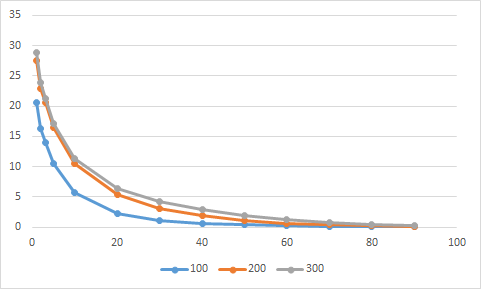
\includegraphics[scale=1]{imagenes/Experimental/DiferenciasAGEU.png}
        \caption{Gráfica asociada a la tabla \ref{diferenciasAGEU}}
        \label{fig:DiferenciasAGEU}
\end{figure}

De la misma forma, en la tabla \ref{DiferenciasCHC} se puede apreciar la media de las diferencias entre las soluciones obtenidas en cada \textit{milestone} de la ejecución del algoritmo CHC con la final (también más visible en la gráfica \ref{fig:DiferenciasCHC}). 

%Diferencias CHC
\begin{table}[]
\begin{tabular}{|cclcclccl|}
\hline
\rowcolor[HTML]{FFFFC7} 
\multicolumn{9}{|c|}{\cellcolor[HTML]{FFFFC7}CHC   450}                                                                                                                                                                                                                                                                                                                                                                                                                                                                                                 \\ \hline
\rowcolor[HTML]{F7EAC7} 
\multicolumn{1}{|c|}{\cellcolor[HTML]{F7EAC7}n}                               & \multicolumn{1}{c|}{\cellcolor[HTML]{F7EAC7}milestone} & \multicolumn{1}{l|}{\cellcolor[HTML]{F7EAC7}Diferencia} & \multicolumn{1}{c|}{\cellcolor[HTML]{F7EAC7}n}                               & \multicolumn{1}{c|}{\cellcolor[HTML]{F7EAC7}milestone} & \multicolumn{1}{l|}{\cellcolor[HTML]{F7EAC7}Diferencia} & \multicolumn{1}{c|}{\cellcolor[HTML]{F7EAC7}n}                               & \multicolumn{1}{c|}{\cellcolor[HTML]{F7EAC7}milestone} & Diferencia \\ \hline
\rowcolor[HTML]{DAE8FC} 
\multicolumn{1}{|c|}{\cellcolor[HTML]{FFFFC7}}                                & \multicolumn{1}{c|}{\cellcolor[HTML]{DAE8FC}1}         & \multicolumn{1}{l|}{\cellcolor[HTML]{DAE8FC}12.8016}    & \multicolumn{1}{c|}{\cellcolor[HTML]{FFFFC7}}                                & \multicolumn{1}{c|}{\cellcolor[HTML]{DAE8FC}1}         & \multicolumn{1}{l|}{\cellcolor[HTML]{DAE8FC}19.8850218} & \multicolumn{1}{c|}{\cellcolor[HTML]{FFFFC7}}                                & \multicolumn{1}{c|}{\cellcolor[HTML]{DAE8FC}1}         & 31.0012675 \\ \cline{2-3} \cline{5-6} \cline{8-9} 
\rowcolor[HTML]{DDFDFF} 
\multicolumn{1}{|c|}{\cellcolor[HTML]{FFFFC7}}                                & \multicolumn{1}{c|}{\cellcolor[HTML]{DDFDFF}2}         & \multicolumn{1}{l|}{\cellcolor[HTML]{DDFDFF}9.87116}    & \multicolumn{1}{c|}{\cellcolor[HTML]{FFFFC7}}                                & \multicolumn{1}{c|}{\cellcolor[HTML]{DDFDFF}2}         & \multicolumn{1}{l|}{\cellcolor[HTML]{DDFDFF}17.2722142} & \multicolumn{1}{c|}{\cellcolor[HTML]{FFFFC7}}                                & \multicolumn{1}{c|}{\cellcolor[HTML]{DDFDFF}2}         & 29.0482187 \\ \cline{2-3} \cline{5-6} \cline{8-9} 
\rowcolor[HTML]{DAE8FC} 
\multicolumn{1}{|c|}{\cellcolor[HTML]{FFFFC7}}                                & \multicolumn{1}{c|}{\cellcolor[HTML]{DAE8FC}3}         & \multicolumn{1}{l|}{\cellcolor[HTML]{DAE8FC}7.03101}    & \multicolumn{1}{c|}{\cellcolor[HTML]{FFFFC7}}                                & \multicolumn{1}{c|}{\cellcolor[HTML]{DAE8FC}3}         & \multicolumn{1}{l|}{\cellcolor[HTML]{DAE8FC}15.6907262} & \multicolumn{1}{c|}{\cellcolor[HTML]{FFFFC7}}                                & \multicolumn{1}{c|}{\cellcolor[HTML]{DAE8FC}3}         & 27.939129  \\ \cline{2-3} \cline{5-6} \cline{8-9} 
\rowcolor[HTML]{DDFDFF} 
\multicolumn{1}{|c|}{\cellcolor[HTML]{FFFFC7}}                                & \multicolumn{1}{c|}{\cellcolor[HTML]{DDFDFF}5}         & \multicolumn{1}{l|}{\cellcolor[HTML]{DDFDFF}4.13105}    & \multicolumn{1}{c|}{\cellcolor[HTML]{FFFFC7}}                                & \multicolumn{1}{c|}{\cellcolor[HTML]{DDFDFF}5}         & \multicolumn{1}{l|}{\cellcolor[HTML]{DDFDFF}13.1825268} & \multicolumn{1}{c|}{\cellcolor[HTML]{FFFFC7}}                                & \multicolumn{1}{c|}{\cellcolor[HTML]{DDFDFF}5}         & 25.9419819 \\ \cline{2-3} \cline{5-6} \cline{8-9} 
\rowcolor[HTML]{DAE8FC} 
\multicolumn{1}{|c|}{\cellcolor[HTML]{FFFFC7}}                                & \multicolumn{1}{c|}{\cellcolor[HTML]{DAE8FC}10}        & \multicolumn{1}{l|}{\cellcolor[HTML]{DAE8FC}0.66658}    & \multicolumn{1}{c|}{\cellcolor[HTML]{FFFFC7}}                                & \multicolumn{1}{c|}{\cellcolor[HTML]{DAE8FC}10}        & \multicolumn{1}{l|}{\cellcolor[HTML]{DAE8FC}5.55650253} & \multicolumn{1}{c|}{\cellcolor[HTML]{FFFFC7}}                                & \multicolumn{1}{c|}{\cellcolor[HTML]{DAE8FC}10}        & 18.8008051 \\ \cline{2-3} \cline{5-6} \cline{8-9} 
\rowcolor[HTML]{DDFDFF} 
\multicolumn{1}{|c|}{\cellcolor[HTML]{FFFFC7}}                                & \multicolumn{1}{c|}{\cellcolor[HTML]{DDFDFF}20}        & \multicolumn{1}{l|}{\cellcolor[HTML]{DDFDFF}0.00171}    & \multicolumn{1}{c|}{\cellcolor[HTML]{FFFFC7}}                                & \multicolumn{1}{c|}{\cellcolor[HTML]{DDFDFF}20}        & \multicolumn{1}{l|}{\cellcolor[HTML]{DDFDFF}0.36295397} & \multicolumn{1}{c|}{\cellcolor[HTML]{FFFFC7}}                                & \multicolumn{1}{c|}{\cellcolor[HTML]{DDFDFF}20}        & 2.2348952  \\ \cline{2-3} \cline{5-6} \cline{8-9} 
\rowcolor[HTML]{DAE8FC} 
\multicolumn{1}{|c|}{\cellcolor[HTML]{FFFFC7}}                                & \multicolumn{1}{c|}{\cellcolor[HTML]{DAE8FC}30}        & \multicolumn{1}{l|}{\cellcolor[HTML]{DAE8FC}2.5E-05}    & \multicolumn{1}{c|}{\cellcolor[HTML]{FFFFC7}}                                & \multicolumn{1}{c|}{\cellcolor[HTML]{DAE8FC}30}        & \multicolumn{1}{l|}{\cellcolor[HTML]{DAE8FC}0.00250816} & \multicolumn{1}{c|}{\cellcolor[HTML]{FFFFC7}}                                & \multicolumn{1}{c|}{\cellcolor[HTML]{DAE8FC}30}        & 0.15429962 \\ \cline{2-3} \cline{5-6} \cline{8-9} 
\rowcolor[HTML]{DDFDFF} 
\multicolumn{1}{|c|}{\cellcolor[HTML]{FFFFC7}}                                & \multicolumn{1}{c|}{\cellcolor[HTML]{DDFDFF}40}        & \multicolumn{1}{l|}{\cellcolor[HTML]{DDFDFF}0}          & \multicolumn{1}{c|}{\cellcolor[HTML]{FFFFC7}}                                & \multicolumn{1}{c|}{\cellcolor[HTML]{DDFDFF}40}        & \multicolumn{1}{l|}{\cellcolor[HTML]{DDFDFF}0.00030503} & \multicolumn{1}{c|}{\cellcolor[HTML]{FFFFC7}}                                & \multicolumn{1}{c|}{\cellcolor[HTML]{DDFDFF}40}        & 0.00179232 \\ \cline{2-3} \cline{5-6} \cline{8-9} 
\rowcolor[HTML]{DAE8FC} 
\multicolumn{1}{|c|}{\cellcolor[HTML]{FFFFC7}}                                & \multicolumn{1}{c|}{\cellcolor[HTML]{DAE8FC}50}        & \multicolumn{1}{l|}{\cellcolor[HTML]{DAE8FC}0}          & \multicolumn{1}{c|}{\cellcolor[HTML]{FFFFC7}}                                & \multicolumn{1}{c|}{\cellcolor[HTML]{DAE8FC}50}        & \multicolumn{1}{l|}{\cellcolor[HTML]{DAE8FC}6.9674E-05} & \multicolumn{1}{c|}{\cellcolor[HTML]{FFFFC7}}                                & \multicolumn{1}{c|}{\cellcolor[HTML]{DAE8FC}50}        & 7.5388E-05 \\ \cline{2-3} \cline{5-6} \cline{8-9} 
\rowcolor[HTML]{DDFDFF} 
\multicolumn{1}{|c|}{\cellcolor[HTML]{FFFFC7}}                                & \multicolumn{1}{c|}{\cellcolor[HTML]{DDFDFF}60}        & \multicolumn{1}{l|}{\cellcolor[HTML]{DDFDFF}0}          & \multicolumn{1}{c|}{\cellcolor[HTML]{FFFFC7}}                                & \multicolumn{1}{c|}{\cellcolor[HTML]{DDFDFF}60}        & \multicolumn{1}{l|}{\cellcolor[HTML]{DDFDFF}0}          & \multicolumn{1}{c|}{\cellcolor[HTML]{FFFFC7}}                                & \multicolumn{1}{c|}{\cellcolor[HTML]{DDFDFF}60}        & 0          \\ \cline{2-3} \cline{5-6} \cline{8-9} 
\rowcolor[HTML]{DAE8FC} 
\multicolumn{1}{|c|}{\cellcolor[HTML]{FFFFC7}}                                & \multicolumn{1}{c|}{\cellcolor[HTML]{DAE8FC}70}        & \multicolumn{1}{l|}{\cellcolor[HTML]{DAE8FC}0}          & \multicolumn{1}{c|}{\cellcolor[HTML]{FFFFC7}}                                & \multicolumn{1}{c|}{\cellcolor[HTML]{DAE8FC}70}        & \multicolumn{1}{l|}{\cellcolor[HTML]{DAE8FC}0}          & \multicolumn{1}{c|}{\cellcolor[HTML]{FFFFC7}}                                & \multicolumn{1}{c|}{\cellcolor[HTML]{DAE8FC}70}        & 0          \\ \cline{2-3} \cline{5-6} \cline{8-9} 
\rowcolor[HTML]{DDFDFF} 
\multicolumn{1}{|c|}{\cellcolor[HTML]{FFFFC7}}                                & \multicolumn{1}{c|}{\cellcolor[HTML]{DDFDFF}80}        & \multicolumn{1}{l|}{\cellcolor[HTML]{DDFDFF}0}          & \multicolumn{1}{c|}{\cellcolor[HTML]{FFFFC7}}                                & \multicolumn{1}{c|}{\cellcolor[HTML]{DDFDFF}80}        & \multicolumn{1}{l|}{\cellcolor[HTML]{DDFDFF}0}          & \multicolumn{1}{c|}{\cellcolor[HTML]{FFFFC7}}                                & \multicolumn{1}{c|}{\cellcolor[HTML]{DDFDFF}80}        & 0          \\ \cline{2-3} \cline{5-6} \cline{8-9} 
\rowcolor[HTML]{DAE8FC} 
\multicolumn{1}{|c|}{\multirow{-13}{*}{\cellcolor[HTML]{FFFFC7}\textbf{100}}} & \multicolumn{1}{c|}{\cellcolor[HTML]{DAE8FC}90}        & \multicolumn{1}{l|}{\cellcolor[HTML]{DAE8FC}0}          & \multicolumn{1}{c|}{\multirow{-13}{*}{\cellcolor[HTML]{FFFFC7}\textbf{200}}} & \multicolumn{1}{c|}{\cellcolor[HTML]{DAE8FC}90}        & \multicolumn{1}{l|}{\cellcolor[HTML]{DAE8FC}0}          & \multicolumn{1}{c|}{\multirow{-13}{*}{\cellcolor[HTML]{FFFFC7}\textbf{300}}} & \multicolumn{1}{c|}{\cellcolor[HTML]{DAE8FC}90}        & 0          \\ \hline
\end{tabular}
\caption{\label{DiferenciasCHC}Diferencias de los resultados de las distintas milestones con respecto a la final para el algoritmo CHC}
\end{table}

\begin{figure}[h]
		\centering
		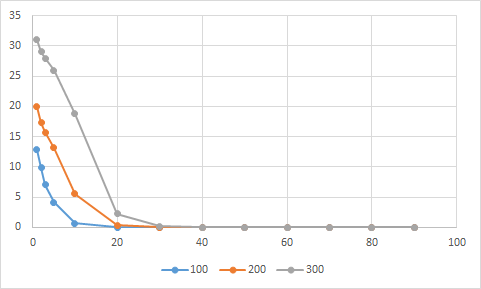
\includegraphics[scale=1]{imagenes/Experimental/DiferenciasCHC.png}
        \caption{Gráfica asociada a la tabla \ref{DiferenciasCHC}}
        \label{fig:DiferenciasCHC}
\end{figure}

Por lo que se puede ver en la tabla \ref{diferenciasAGEU} no se puede decir que converja prematuramente, de hecho en todo momento realiza mejoras significativas. 
Esto se puede observar en el hecho de que las diferencias a la última solución van disminuyendo en gran medida en cada una de las \textit{milestones}. 

Sin embargo, en la tabla \ref{DiferenciasCHC} se tiene que las soluciones convergen rápidamente a la solución final antes de llegar siquiera el 50\% de la ejecución total. 
De esto se puede inferir que los mecanismos de aumento de la diversidad de CHC no son de mucha utilidad en nuestro caso. 
También se debe tener en cuenta que estamos usando una modificación de CHC donde no se reinicia la población, ya que se prevee su rápida convergencia, lo que causaría una gran cantidad de reinicios y, por tanto, evaluaciones, las cuales estamos intentando mantener al mínimo. 
En contrapartida a no usar reinicio de población, se mantiene la mutación de las soluciones con el fin de aportar más diversidad. 
A vista de los resultados se puede entender que esto no es suficiente para mantener la diversidad. 

Por otra parte, si nos fijamos en la gráfica \ref{fig:AGEUvsCHC} se puede ver cómo el algoritmo CHC es mejor que el AGEU mientras que se siguen produciendo cambios, es decir, antes de que se produzca el 50\% de la ejecución. 
Por lo que se considerará posteriormente una mezcla de ambos algoritmos, con el fin de aprovechar los buenos resultados iniciales del CHC y la capacidad de no converger rápidamente que presenta AGEU con el fin de tener un buen punto de partida.

\section{Incorporación del histórico}

La primera modificación que se propone es la introducción de un histórico \ref{alg:Historico_Estructura}, explicado en la primera sección del capítulo anterior. 
La principal motivación de esta modificación es incidir en la explotación de las buenas soluciones, ya que se almacenarán los elementos más predominantes en las mejores soluciones y en las peores, con el fin de reincidir con mayor frecuencia en los primeros y rehuir de los segundos. 

Obviamente, este histórico deberá tener un proceso de aprendizaje (en el que almacena todas las soluciones distintas para luego discernir cuáles son las mejores y cuáles las peores y sus respectivos elementos) y un proceso de reacción, en la que pondrá en práctica la información aprendida en la fase anterior. 
Con el fin de que no sea un único procedimiento y pueda ir aprendiendo a lo largo de la ejecución (para intentar evitar quedarse en máximos locales), estas dos fases se irán turnando cada 50 generaciones. 

Para poner a prueba su utilidad, se estudian los resultados obtenidos de aplicar el histórico solo al operador de reparación (si tiene que añadir elementos, elegirá los mejores; si tiene que eliminar elementos, elegirá los peores), solo a la mutación (tiene prioridad insertar mejores elementos y eliminar peores) y a ambos a la vez. 
Los resultados de este estudio se muestran en la tablas \ref{HistMut}, \ref{HistCruce} y \ref{GACEPv1} y, más visualmente, en la gráfica \ref{fig:Historico}.

\begin{figure}
     \centering
     \begin{subfigure}[b]{0.45\textwidth}
         \centering
         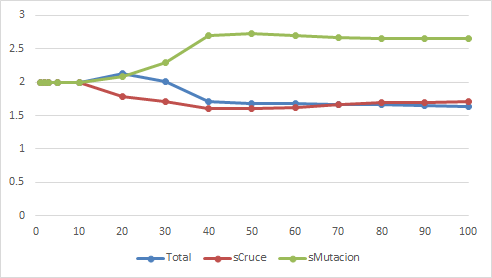
\includegraphics[width=\textwidth]{imagenes/Experimental/Historico.png}
         \caption{Ranking durante todas las \textit{milestones}}
         \label{fig:Historico_lineas}
     \end{subfigure}
     \hfill
     \begin{subfigure}[b]{0.45\textwidth}
         \centering
         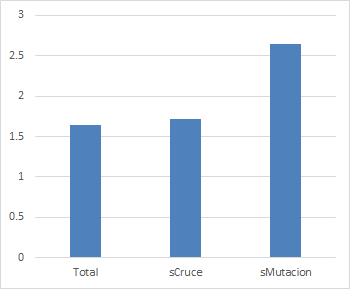
\includegraphics[width=\textwidth]{imagenes/Experimental/barras/Historico.png}
         \caption{Ranking final}
         \label{fig:Historico_barras}
     \end{subfigure}
        \caption{Comparación de las distintas versiones del histórico}
        \label{fig:Historico}
\end{figure}

En esta gráfica \ref{fig:Historico} podemos apreciar que las mejores opciones son aplicarlo solo al cruce o a ambos; de hecho, por muy poco se tiene que aplicar ambas modificaciones es lo mejor. 
El uso de ambas opciones también viene justificado por un intento de mantener la consistencia, y porque es posible que en algún momento del desarrollo se puedan realizar más modificaciones a la mutación de las que el histórico se podría aprovechar. 

Además, que cuando solo se aplique el histórico a la mutación de los peores resultados con diferencia es una primera indicación de que la introducción del histórico ha supuesto una mejora al modelo original.
Esto se debe a que realmente la mutación se produce un número muy bajo de veces y no suele producir grandes cambios, por lo que si es lo único que se modifica, es muy probable que no se distancie mucho de los resultados originales. 
Para confirmar esta idea y poder asegurarnos de que se ha dado un paso en una dirección correcta, comparamos en la gráfica \ref{fig:AGEUvsGACEPv1} los resultados originales y los de aplicar el histórico a ambos operadores. 

\begin{figure}
     \centering
     \begin{subfigure}[b]{0.45\textwidth}
         \centering
         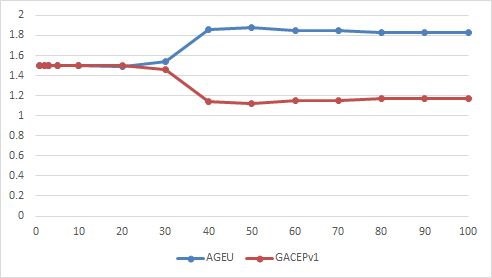
\includegraphics[width=\textwidth]{imagenes/Experimental/AGEUvsGACEPv1.png}
         \caption{Ranking durante todas las \textit{milestones}}
         \label{fig:AGEUvsGACEPv1_lineas}
     \end{subfigure}
     \hfill
     \begin{subfigure}[b]{0.45\textwidth}
         \centering
         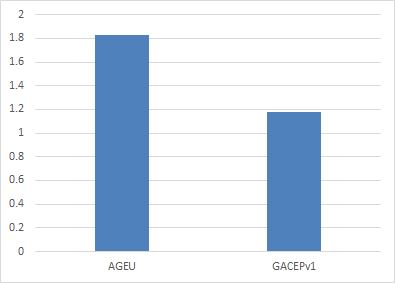
\includegraphics[width=\textwidth]{imagenes/Experimental/barras/AGEUvsGACEPv1.png}
         \caption{Ranking final}
         \label{fig:AGEUvsGACEPv1_barras}
     \end{subfigure}
        \caption{Comparación de los resultados del AGEU y GACEPv1}
        \label{fig:AGEUvsGACEPv1}
\end{figure}

Con esta gráfica \ref{fig:AGEUvsGACEPv1} quedan confirmadas nuestras suposiciones. 
Es importante mencionar que en sus primeras iteraciones ambos algoritmos obtienen los mismos resultados ya que se comportan de la misma forma. 
Recordemos que cada fase del histórico ocupa 50 iteraciones, por lo que durante las primeras 50 iteraciones va a mantener el mismo comportamiento que AGEU, con la excepción de que va a ir almacenando las soluciones para su posterior análisis. 
Estas 50 iteraciones suponen un poco más del 10\% inicial de las iteraciones totales, por lo que es obvio que para todas estas \textit{milestones} sus resultados van a ser iguales. 
También cabe la pena mencionar que en el momento en el que difieren los resultados de los algoritmos, su clasificación se mantiene casi constante, por lo que queda claro que el uso del histórico hace que el algoritmo sea consistentemente mejor.  

Es más, con esta modificación podemos crear las bases de lo que será nuestro nuevo algoritmo, al cual llamaremos \textbf{GACEP} (\textbf{\textit{Genetic Algorithm for Combinatory Expensive Problem}}). 
Para establecer una notación común entre las distintas modificaciones, todas se nombrarán de la forma ``GACEPv\texttt{x}'', donde \texttt{x} se sustituirá por el número de la versión. 
En este caso, el introducir el histórico al AG lo llamaremos \textbf{GACEPv1}.

Los resultados de la ejecución de este algoritmo vienen recopilados en la tabla \ref{GACEPv1}.

A continuación haremos lo mismo que para los algoritmos de referencia y observaremos si se ha producido algún tipo de convergencia prematura. 
Esto se puede ver en la tabla \ref{DiferenciasGACEPv1} y en su gráfica asociada \ref{fig:DiferenciasGACEPv1}.

%Diferencias GACEP
\begin{table}[]
\begin{tabular}{|cclcclccl|}
\hline
\rowcolor[HTML]{FFFFC7} 
\multicolumn{9}{|c|}{\cellcolor[HTML]{FFFFC7}GACEPv1}                                                                                                                                                                                                                                                                                                                                                                                                                                                                        \\ \hline
\rowcolor[HTML]{F7EAC7} 
\multicolumn{1}{|c|}{\cellcolor[HTML]{F7EAC7}n}                      & \multicolumn{1}{c|}{\cellcolor[HTML]{F7EAC7}milestone} & \multicolumn{1}{l|}{\cellcolor[HTML]{F7EAC7}Diferencia} & \multicolumn{1}{c|}{\cellcolor[HTML]{F7EAC7}n}                      & \multicolumn{1}{c|}{\cellcolor[HTML]{F7EAC7}milestone} & \multicolumn{1}{l|}{\cellcolor[HTML]{F7EAC7}Diferencia} & \multicolumn{1}{c|}{\cellcolor[HTML]{F7EAC7}n}                      & \multicolumn{1}{c|}{\cellcolor[HTML]{F7EAC7}milestone} & Diferencia \\ \hline
\rowcolor[HTML]{DAE8FC} 
\multicolumn{1}{|c|}{\cellcolor[HTML]{FFFFC7}}                       & \multicolumn{1}{c|}{\cellcolor[HTML]{DAE8FC}1}         & \multicolumn{1}{l|}{\cellcolor[HTML]{DAE8FC}24.8702}    & \multicolumn{1}{c|}{\cellcolor[HTML]{FFFFC7}}                       & \multicolumn{1}{c|}{\cellcolor[HTML]{DAE8FC}1}         & \multicolumn{1}{l|}{\cellcolor[HTML]{DAE8FC}28.9265669} & \multicolumn{1}{c|}{\cellcolor[HTML]{FFFFC7}}                       & \multicolumn{1}{c|}{\cellcolor[HTML]{DAE8FC}1}         & 28.4705381 \\ \cline{2-3} \cline{5-6} \cline{8-9} 
\rowcolor[HTML]{DDFDFF} 
\multicolumn{1}{|c|}{\cellcolor[HTML]{FFFFC7}}                       & \multicolumn{1}{c|}{\cellcolor[HTML]{DDFDFF}2}         & \multicolumn{1}{l|}{\cellcolor[HTML]{DDFDFF}20.8839}    & \multicolumn{1}{c|}{\cellcolor[HTML]{FFFFC7}}                       & \multicolumn{1}{c|}{\cellcolor[HTML]{DDFDFF}2}         & \multicolumn{1}{l|}{\cellcolor[HTML]{DDFDFF}24.473429}  & \multicolumn{1}{c|}{\cellcolor[HTML]{FFFFC7}}                       & \multicolumn{1}{c|}{\cellcolor[HTML]{DDFDFF}2}         & 23.6064829 \\ \cline{2-3} \cline{5-6} \cline{8-9} 
\rowcolor[HTML]{DAE8FC} 
\multicolumn{1}{|c|}{\cellcolor[HTML]{FFFFC7}}                       & \multicolumn{1}{c|}{\cellcolor[HTML]{DAE8FC}3}         & \multicolumn{1}{l|}{\cellcolor[HTML]{DAE8FC}18.6934}    & \multicolumn{1}{c|}{\cellcolor[HTML]{FFFFC7}}                       & \multicolumn{1}{c|}{\cellcolor[HTML]{DAE8FC}3}         & \multicolumn{1}{l|}{\cellcolor[HTML]{DAE8FC}22.2164778} & \multicolumn{1}{c|}{\cellcolor[HTML]{FFFFC7}}                       & \multicolumn{1}{c|}{\cellcolor[HTML]{DAE8FC}3}         & 21.0057888 \\ \cline{2-3} \cline{5-6} \cline{8-9} 
\rowcolor[HTML]{DDFDFF} 
\multicolumn{1}{|c|}{\cellcolor[HTML]{FFFFC7}}                       & \multicolumn{1}{c|}{\cellcolor[HTML]{DDFDFF}5}         & \multicolumn{1}{l|}{\cellcolor[HTML]{DDFDFF}15.4131}    & \multicolumn{1}{c|}{\cellcolor[HTML]{FFFFC7}}                       & \multicolumn{1}{c|}{\cellcolor[HTML]{DDFDFF}5}         & \multicolumn{1}{l|}{\cellcolor[HTML]{DDFDFF}18.2724015} & \multicolumn{1}{c|}{\cellcolor[HTML]{FFFFC7}}                       & \multicolumn{1}{c|}{\cellcolor[HTML]{DDFDFF}5}         & 17.0150669 \\ \cline{2-3} \cline{5-6} \cline{8-9} 
\rowcolor[HTML]{DAE8FC} 
\multicolumn{1}{|c|}{\cellcolor[HTML]{FFFFC7}}                       & \multicolumn{1}{c|}{\cellcolor[HTML]{DAE8FC}10}        & \multicolumn{1}{l|}{\cellcolor[HTML]{DAE8FC}10.9019}    & \multicolumn{1}{c|}{\cellcolor[HTML]{FFFFC7}}                       & \multicolumn{1}{c|}{\cellcolor[HTML]{DAE8FC}10}        & \multicolumn{1}{l|}{\cellcolor[HTML]{DAE8FC}12.4140872} & \multicolumn{1}{c|}{\cellcolor[HTML]{FFFFC7}}                       & \multicolumn{1}{c|}{\cellcolor[HTML]{DAE8FC}10}        & 11.1442233 \\ \cline{2-3} \cline{5-6} \cline{8-9} 
\rowcolor[HTML]{DDFDFF} 
\multicolumn{1}{|c|}{\cellcolor[HTML]{FFFFC7}}                       & \multicolumn{1}{c|}{\cellcolor[HTML]{DDFDFF}20}        & \multicolumn{1}{l|}{\cellcolor[HTML]{DDFDFF}5.64471}    & \multicolumn{1}{c|}{\cellcolor[HTML]{FFFFC7}}                       & \multicolumn{1}{c|}{\cellcolor[HTML]{DDFDFF}20}        & \multicolumn{1}{l|}{\cellcolor[HTML]{DDFDFF}8.14923733} & \multicolumn{1}{c|}{\cellcolor[HTML]{FFFFC7}}                       & \multicolumn{1}{c|}{\cellcolor[HTML]{DDFDFF}20}        & 6.84098075 \\ \cline{2-3} \cline{5-6} \cline{8-9} 
\rowcolor[HTML]{DAE8FC} 
\multicolumn{1}{|c|}{\cellcolor[HTML]{FFFFC7}}                       & \multicolumn{1}{c|}{\cellcolor[HTML]{DAE8FC}30}        & \multicolumn{1}{l|}{\cellcolor[HTML]{DAE8FC}4.10969}    & \multicolumn{1}{c|}{\cellcolor[HTML]{FFFFC7}}                       & \multicolumn{1}{c|}{\cellcolor[HTML]{DAE8FC}30}        & \multicolumn{1}{l|}{\cellcolor[HTML]{DAE8FC}5.35892582} & \multicolumn{1}{c|}{\cellcolor[HTML]{FFFFC7}}                       & \multicolumn{1}{c|}{\cellcolor[HTML]{DAE8FC}30}        & 4.4650068  \\ \cline{2-3} \cline{5-6} \cline{8-9} 
\rowcolor[HTML]{DDFDFF} 
\multicolumn{1}{|c|}{\cellcolor[HTML]{FFFFC7}}                       & \multicolumn{1}{c|}{\cellcolor[HTML]{DDFDFF}40}        & \multicolumn{1}{l|}{\cellcolor[HTML]{DDFDFF}1.43438}    & \multicolumn{1}{c|}{\cellcolor[HTML]{FFFFC7}}                       & \multicolumn{1}{c|}{\cellcolor[HTML]{DDFDFF}40}        & \multicolumn{1}{l|}{\cellcolor[HTML]{DDFDFF}2.30317627} & \multicolumn{1}{c|}{\cellcolor[HTML]{FFFFC7}}                       & \multicolumn{1}{c|}{\cellcolor[HTML]{DDFDFF}40}        & 2.05939817 \\ \cline{2-3} \cline{5-6} \cline{8-9} 
\rowcolor[HTML]{DAE8FC} 
\multicolumn{1}{|c|}{\cellcolor[HTML]{FFFFC7}}                       & \multicolumn{1}{c|}{\cellcolor[HTML]{DAE8FC}50}        & \multicolumn{1}{l|}{\cellcolor[HTML]{DAE8FC}0.63711}    & \multicolumn{1}{c|}{\cellcolor[HTML]{FFFFC7}}                       & \multicolumn{1}{c|}{\cellcolor[HTML]{DAE8FC}50}        & \multicolumn{1}{l|}{\cellcolor[HTML]{DAE8FC}0.97838195} & \multicolumn{1}{c|}{\cellcolor[HTML]{FFFFC7}}                       & \multicolumn{1}{c|}{\cellcolor[HTML]{DAE8FC}50}        & 1.03637898 \\ \cline{2-3} \cline{5-6} \cline{8-9} 
\rowcolor[HTML]{DDFDFF} 
\multicolumn{1}{|c|}{\cellcolor[HTML]{FFFFC7}}                       & \multicolumn{1}{c|}{\cellcolor[HTML]{DDFDFF}60}        & \multicolumn{1}{l|}{\cellcolor[HTML]{DDFDFF}0.34425}    & \multicolumn{1}{c|}{\cellcolor[HTML]{FFFFC7}}                       & \multicolumn{1}{c|}{\cellcolor[HTML]{DDFDFF}60}        & \multicolumn{1}{l|}{\cellcolor[HTML]{DDFDFF}0.61345105} & \multicolumn{1}{c|}{\cellcolor[HTML]{FFFFC7}}                       & \multicolumn{1}{c|}{\cellcolor[HTML]{DDFDFF}60}        & 0.65967857 \\ \cline{2-3} \cline{5-6} \cline{8-9} 
\rowcolor[HTML]{DAE8FC} 
\multicolumn{1}{|c|}{\cellcolor[HTML]{FFFFC7}}                       & \multicolumn{1}{c|}{\cellcolor[HTML]{DAE8FC}70}        & \multicolumn{1}{l|}{\cellcolor[HTML]{DAE8FC}0.18073}    & \multicolumn{1}{c|}{\cellcolor[HTML]{FFFFC7}}                       & \multicolumn{1}{c|}{\cellcolor[HTML]{DAE8FC}70}        & \multicolumn{1}{l|}{\cellcolor[HTML]{DAE8FC}0.22987072} & \multicolumn{1}{c|}{\cellcolor[HTML]{FFFFC7}}                       & \multicolumn{1}{c|}{\cellcolor[HTML]{DAE8FC}70}        & 0.32037747 \\ \cline{2-3} \cline{5-6} \cline{8-9} 
\rowcolor[HTML]{DDFDFF} 
\multicolumn{1}{|c|}{\cellcolor[HTML]{FFFFC7}}                       & \multicolumn{1}{c|}{\cellcolor[HTML]{DDFDFF}80}        & \multicolumn{1}{l|}{\cellcolor[HTML]{DDFDFF}0.09555}    & \multicolumn{1}{c|}{\cellcolor[HTML]{FFFFC7}}                       & \multicolumn{1}{c|}{\cellcolor[HTML]{DDFDFF}80}        & \multicolumn{1}{l|}{\cellcolor[HTML]{DDFDFF}0.17789507} & \multicolumn{1}{c|}{\cellcolor[HTML]{FFFFC7}}                       & \multicolumn{1}{c|}{\cellcolor[HTML]{DDFDFF}80}        & 0.21069325 \\ \cline{2-3} \cline{5-6} \cline{8-9} 
\rowcolor[HTML]{DAE8FC} 
\multicolumn{1}{|c|}{\multirow{-13}{*}{\cellcolor[HTML]{FFFFC7}100}} & \multicolumn{1}{c|}{\cellcolor[HTML]{DAE8FC}90}        & \multicolumn{1}{l|}{\cellcolor[HTML]{DAE8FC}-0.0002}    & \multicolumn{1}{c|}{\multirow{-13}{*}{\cellcolor[HTML]{FFFFC7}200}} & \multicolumn{1}{c|}{\cellcolor[HTML]{DAE8FC}90}        & \multicolumn{1}{l|}{\cellcolor[HTML]{DAE8FC}0.02225991} & \multicolumn{1}{c|}{\multirow{-13}{*}{\cellcolor[HTML]{FFFFC7}300}} & \multicolumn{1}{c|}{\cellcolor[HTML]{DAE8FC}90}        & 0.04461874 \\ \hline
\end{tabular}
\caption{\label{DiferenciasGACEPv1}Diferencias de los resultados de las distintas milestones con respecto a la final para el algoritmo GACEPv1}
\end{table}

\begin{figure}[h]
		\centering
		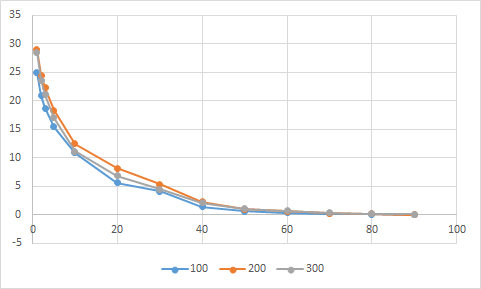
\includegraphics[scale=1]{imagenes/Experimental/DiferenciasGACEPv1.png}
        \caption{Gráfica asociada a la tabla \ref{DiferenciasGACEPv1}}
        \label{fig:DiferenciasGACEPv1}
\end{figure}

En la tabla \ref{DiferenciasGACEPv1} se puede ver que GACEP tiene un comportamiento similar con respecto a la progresión de las mejores soluciones a lo largo de la ejecución que el algoritmo base AGEU. 
Se observa que no se produce ninguna convergencia prematura, aunque es cierto que en la segunda mitad de las evaluaciones se producen muchos menos cambios que en el resto. 



\section{Uso de GRASP}

La modificación anterior tenía como objetivo aumentar la explotación de los buenos resultados. 
Para volver a conseguir un buen balance de explotación y exploración en el algoritmo lo siguiente que debemos pensar es qué clase de modificación se podría introducir de forma que aumentase la diversidad de la población y/o de las soluciones a considerar. 

La siguiente modificación que se plantea es la sustitución del uso del algoritmo Greedy por una variante suya: GRASP. 
Esta modificación solo tiene sentido usarla en el operador de reparación en la fase de aprendizaje del histórico. 
Esto es porque el único sitio donde se utiliza Greedy es en el operador de reparación, que intenta introducir siempre el mejor elemento a la solución y eliminar el peor. 
Durante la fase de acción del histórico ya realiza de por si un procedimiento similar al del GRASP \ref{alg:GRASP}, ya que le da prioridad a introducir alguno (sin comprobar si es verdaderamente el mejor) de los mejores elementos aprendidos y eliminar alguno (sin comprobar si verdaderamente es el peor) de los peores elementos aprendidos. 

El objetivo de esta modificación es introducir un operador que permita diversificar la población, eliminando el determinismo de siempre elegir las mismos elementos. 
De esta forma, somos capaces de darle más importancia a la parte de exploración del algoritmo, pero siempre manteniendo que las soluciones sigan intentando ser lo mejor posible. 

Por tanto, \textbf{GACEPv2} será resultado de añadir un operador GRASP al operador de reparación de GACEPv1.

Los resultados de la ejecución del algoritmo GACEP con esta modificación pueden verse en la tabla \ref{GACEPv2}. 

Con esto, debemos comprobar si realmente se ha producido una mejora con respecto a la modificación anterior. 
Para ello compararemos sus resultados y estableceremos un \textit{ranking}, siendo la gráfica correspondiente a esta comparación la gráfica \ref{fig:AGEUvsGACEPv1}. 


\begin{figure}[h]
     \centering
     \begin{subfigure}[b]{0.45\textwidth}
         \centering
         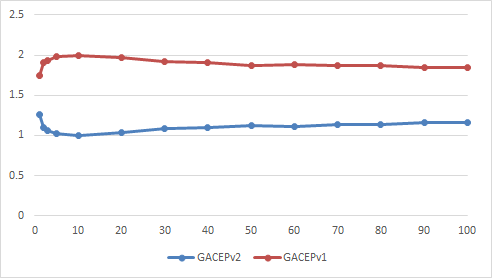
\includegraphics[width=\textwidth]{imagenes/Experimental/GRASPvswoGRASP.png}
         \caption{Ranking durante todas las \textit{milestones}}
         \label{fig:AGEUvsGACEPv1_lineas}
     \end{subfigure}
     \hfill
     \begin{subfigure}[b]{0.45\textwidth}
         \centering
         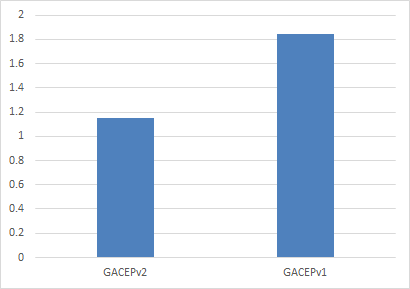
\includegraphics[width=\textwidth]{imagenes/Experimental/barras/GRASPvswoGRASP.png}
         \caption{Ranking final}
         \label{fig:AGEUvsGACEPv1_barras}
     \end{subfigure}
        \caption{Comparación de los resultados del GACEPv1 y GACEPv2}
        \label{fig:AGEUvsGACEPv1}
\end{figure}

En esta gráfica \ref{fig:AGEUvsGACEPv1} se puede ver cómo la nueva versión, introduciendo GRASP, es consistentemente mejor que la versión anterior. 
Es más, se puede afirmar que es mejor en casi todos los datos utilizados. 
Por lo tanto, se procederá a continuar con el desarrollo de nuestro algoritmo sobre esta nueva versión.

A continuación, se mostrará una tabla \ref{DiferenciasGACEP_GRASP} que almacena la media de las diferencias de los resultados de cada \textit{milestone} con respecto a la final, con el fin de comprobar si podemos sacar información sobre la convergencia de las soluciones en el tiempo. 

%GACEPv2 - Diferencias
\begin{table}[]
\begin{tabular}{|ccrccrccr|}
\hline
\rowcolor[HTML]{FFFFC7} 
\multicolumn{9}{|c|}{\cellcolor[HTML]{FFFFC7}GACEPv2}                                                                                                                                                                                                                                                                                                                                                                                                                                                                                                                     \\ \hline
\rowcolor[HTML]{F7EAC7} 
\multicolumn{1}{|c|}{\cellcolor[HTML]{F7EAC7}n}                      & \multicolumn{1}{c|}{\cellcolor[HTML]{F7EAC7}milestone} & \multicolumn{1}{l|}{\cellcolor[HTML]{F7EAC7}Diferencia} & \multicolumn{1}{c|}{\cellcolor[HTML]{F7EAC7}n}                      & \multicolumn{1}{c|}{\cellcolor[HTML]{F7EAC7}milestone} & \multicolumn{1}{l|}{\cellcolor[HTML]{F7EAC7}Diferencia} & \multicolumn{1}{c|}{\cellcolor[HTML]{F7EAC7}n}                      & \multicolumn{1}{c|}{\cellcolor[HTML]{F7EAC7}milestone} & \multicolumn{1}{l|}{\cellcolor[HTML]{F7EAC7}Diferencia} \\ \hline
\rowcolor[HTML]{DAE8FC} 
\multicolumn{1}{|c|}{\cellcolor[HTML]{FFFFC7}}                       & \multicolumn{1}{c|}{\cellcolor[HTML]{DAE8FC}1}         & \multicolumn{1}{r|}{\cellcolor[HTML]{DAE8FC}25.3737}    & \multicolumn{1}{c|}{\cellcolor[HTML]{FFFFC7}}                       & \multicolumn{1}{c|}{\cellcolor[HTML]{DAE8FC}1}         & \multicolumn{1}{r|}{\cellcolor[HTML]{DAE8FC}29.8461881} & \multicolumn{1}{c|}{\cellcolor[HTML]{FFFFC7}}                       & \multicolumn{1}{c|}{\cellcolor[HTML]{DAE8FC}1}         & 28.9145096                                              \\ \cline{2-3} \cline{5-6} \cline{8-9} 
\rowcolor[HTML]{DDFDFF} 
\multicolumn{1}{|c|}{\cellcolor[HTML]{FFFFC7}}                       & \multicolumn{1}{c|}{\cellcolor[HTML]{DDFDFF}2}         & \multicolumn{1}{r|}{\cellcolor[HTML]{DDFDFF}20.6761}    & \multicolumn{1}{c|}{\cellcolor[HTML]{FFFFC7}}                       & \multicolumn{1}{c|}{\cellcolor[HTML]{DDFDFF}2}         & \multicolumn{1}{r|}{\cellcolor[HTML]{DDFDFF}24.9678186} & \multicolumn{1}{c|}{\cellcolor[HTML]{FFFFC7}}                       & \multicolumn{1}{c|}{\cellcolor[HTML]{DDFDFF}2}         & 24.0603906                                              \\ \cline{2-3} \cline{5-6} \cline{8-9} 
\rowcolor[HTML]{DAE8FC} 
\multicolumn{1}{|c|}{\cellcolor[HTML]{FFFFC7}}                       & \multicolumn{1}{c|}{\cellcolor[HTML]{DAE8FC}3}         & \multicolumn{1}{r|}{\cellcolor[HTML]{DAE8FC}18.4198}    & \multicolumn{1}{c|}{\cellcolor[HTML]{FFFFC7}}                       & \multicolumn{1}{c|}{\cellcolor[HTML]{DAE8FC}3}         & \multicolumn{1}{r|}{\cellcolor[HTML]{DAE8FC}22.561253}  & \multicolumn{1}{c|}{\cellcolor[HTML]{FFFFC7}}                       & \multicolumn{1}{c|}{\cellcolor[HTML]{DAE8FC}3}         & 21.4992992                                              \\ \cline{2-3} \cline{5-6} \cline{8-9} 
\rowcolor[HTML]{DDFDFF} 
\multicolumn{1}{|c|}{\cellcolor[HTML]{FFFFC7}}                       & \multicolumn{1}{c|}{\cellcolor[HTML]{DDFDFF}5}         & \multicolumn{1}{r|}{\cellcolor[HTML]{DDFDFF}14.7471}    & \multicolumn{1}{c|}{\cellcolor[HTML]{FFFFC7}}                       & \multicolumn{1}{c|}{\cellcolor[HTML]{DDFDFF}5}         & \multicolumn{1}{r|}{\cellcolor[HTML]{DDFDFF}18.4329667} & \multicolumn{1}{c|}{\cellcolor[HTML]{FFFFC7}}                       & \multicolumn{1}{c|}{\cellcolor[HTML]{DDFDFF}5}         & 17.1360467                                              \\ \cline{2-3} \cline{5-6} \cline{8-9} 
\rowcolor[HTML]{DAE8FC} 
\multicolumn{1}{|c|}{\cellcolor[HTML]{FFFFC7}}                       & \multicolumn{1}{c|}{\cellcolor[HTML]{DAE8FC}10}        & \multicolumn{1}{r|}{\cellcolor[HTML]{DAE8FC}9.94967}    & \multicolumn{1}{c|}{\cellcolor[HTML]{FFFFC7}}                       & \multicolumn{1}{c|}{\cellcolor[HTML]{DAE8FC}10}        & \multicolumn{1}{r|}{\cellcolor[HTML]{DAE8FC}11.9316113} & \multicolumn{1}{c|}{\cellcolor[HTML]{FFFFC7}}                       & \multicolumn{1}{c|}{\cellcolor[HTML]{DAE8FC}10}        & 10.5285922                                              \\ \cline{2-3} \cline{5-6} \cline{8-9} 
\rowcolor[HTML]{DDFDFF} 
\multicolumn{1}{|c|}{\cellcolor[HTML]{FFFFC7}}                       & \multicolumn{1}{c|}{\cellcolor[HTML]{DDFDFF}20}        & \multicolumn{1}{r|}{\cellcolor[HTML]{DDFDFF}5.62915}    & \multicolumn{1}{c|}{\cellcolor[HTML]{FFFFC7}}                       & \multicolumn{1}{c|}{\cellcolor[HTML]{DDFDFF}20}        & \multicolumn{1}{r|}{\cellcolor[HTML]{DDFDFF}7.98414965} & \multicolumn{1}{c|}{\cellcolor[HTML]{FFFFC7}}                       & \multicolumn{1}{c|}{\cellcolor[HTML]{DDFDFF}20}        & 6.88853082                                              \\ \cline{2-3} \cline{5-6} \cline{8-9} 
\rowcolor[HTML]{DAE8FC} 
\multicolumn{1}{|c|}{\cellcolor[HTML]{FFFFC7}}                       & \multicolumn{1}{c|}{\cellcolor[HTML]{DAE8FC}30}        & \multicolumn{1}{r|}{\cellcolor[HTML]{DAE8FC}4.38901}    & \multicolumn{1}{c|}{\cellcolor[HTML]{FFFFC7}}                       & \multicolumn{1}{c|}{\cellcolor[HTML]{DAE8FC}30}        & \multicolumn{1}{r|}{\cellcolor[HTML]{DAE8FC}5.14003393} & \multicolumn{1}{c|}{\cellcolor[HTML]{FFFFC7}}                       & \multicolumn{1}{c|}{\cellcolor[HTML]{DAE8FC}30}        & 4.43403031                                              \\ \cline{2-3} \cline{5-6} \cline{8-9} 
\rowcolor[HTML]{DDFDFF} 
\multicolumn{1}{|c|}{\cellcolor[HTML]{FFFFC7}}                       & \multicolumn{1}{c|}{\cellcolor[HTML]{DDFDFF}40}        & \multicolumn{1}{r|}{\cellcolor[HTML]{DDFDFF}0.7794}     & \multicolumn{1}{c|}{\cellcolor[HTML]{FFFFC7}}                       & \multicolumn{1}{c|}{\cellcolor[HTML]{DDFDFF}40}        & \multicolumn{1}{r|}{\cellcolor[HTML]{DDFDFF}2.28877565} & \multicolumn{1}{c|}{\cellcolor[HTML]{FFFFC7}}                       & \multicolumn{1}{c|}{\cellcolor[HTML]{DDFDFF}40}        & 2.14374372                                              \\ \cline{2-3} \cline{5-6} \cline{8-9} 
\rowcolor[HTML]{DAE8FC} 
\multicolumn{1}{|c|}{\cellcolor[HTML]{FFFFC7}}                       & \multicolumn{1}{c|}{\cellcolor[HTML]{DAE8FC}50}        & \multicolumn{1}{r|}{\cellcolor[HTML]{DAE8FC}0.21656}    & \multicolumn{1}{c|}{\cellcolor[HTML]{FFFFC7}}                       & \multicolumn{1}{c|}{\cellcolor[HTML]{DAE8FC}50}        & \multicolumn{1}{r|}{\cellcolor[HTML]{DAE8FC}1.07903317} & \multicolumn{1}{c|}{\cellcolor[HTML]{FFFFC7}}                       & \multicolumn{1}{c|}{\cellcolor[HTML]{DAE8FC}50}        & 1.15285329                                              \\ \cline{2-3} \cline{5-6} \cline{8-9} 
\rowcolor[HTML]{DDFDFF} 
\multicolumn{1}{|c|}{\cellcolor[HTML]{FFFFC7}}                       & \multicolumn{1}{c|}{\cellcolor[HTML]{DDFDFF}60}        & \multicolumn{1}{r|}{\cellcolor[HTML]{DDFDFF}0.06538}    & \multicolumn{1}{c|}{\cellcolor[HTML]{FFFFC7}}                       & \multicolumn{1}{c|}{\cellcolor[HTML]{DDFDFF}60}        & \multicolumn{1}{r|}{\cellcolor[HTML]{DDFDFF}0.42600859} & \multicolumn{1}{c|}{\cellcolor[HTML]{FFFFC7}}                       & \multicolumn{1}{c|}{\cellcolor[HTML]{DDFDFF}60}        & 0.59987399                                              \\ \cline{2-3} \cline{5-6} \cline{8-9} 
\rowcolor[HTML]{DAE8FC} 
\multicolumn{1}{|c|}{\cellcolor[HTML]{FFFFC7}}                       & \multicolumn{1}{c|}{\cellcolor[HTML]{DAE8FC}70}        & \multicolumn{1}{r|}{\cellcolor[HTML]{DAE8FC}0.01904}    & \multicolumn{1}{c|}{\cellcolor[HTML]{FFFFC7}}                       & \multicolumn{1}{c|}{\cellcolor[HTML]{DAE8FC}70}        & \multicolumn{1}{r|}{\cellcolor[HTML]{DAE8FC}0.04685168} & \multicolumn{1}{c|}{\cellcolor[HTML]{FFFFC7}}                       & \multicolumn{1}{c|}{\cellcolor[HTML]{DAE8FC}70}        & 0.17475741                                              \\ \cline{2-3} \cline{5-6} \cline{8-9} 
\rowcolor[HTML]{DDFDFF} 
\multicolumn{1}{|c|}{\cellcolor[HTML]{FFFFC7}}                       & \multicolumn{1}{c|}{\cellcolor[HTML]{DDFDFF}80}        & \multicolumn{1}{r|}{\cellcolor[HTML]{DDFDFF}0.00528}    & \multicolumn{1}{c|}{\cellcolor[HTML]{FFFFC7}}                       & \multicolumn{1}{c|}{\cellcolor[HTML]{DDFDFF}80}        & \multicolumn{1}{r|}{\cellcolor[HTML]{DDFDFF}0.01998544} & \multicolumn{1}{c|}{\cellcolor[HTML]{FFFFC7}}                       & \multicolumn{1}{c|}{\cellcolor[HTML]{DDFDFF}80}        & 0.10914333                                              \\ \cline{2-3} \cline{5-6} \cline{8-9} 
\rowcolor[HTML]{DAE8FC} 
\multicolumn{1}{|c|}{\multirow{-13}{*}{\cellcolor[HTML]{FFFFC7}100}} & \multicolumn{1}{c|}{\cellcolor[HTML]{DAE8FC}90}        & \multicolumn{1}{r|}{\cellcolor[HTML]{DAE8FC}-0.0014}    & \multicolumn{1}{c|}{\multirow{-13}{*}{\cellcolor[HTML]{FFFFC7}200}} & \multicolumn{1}{c|}{\cellcolor[HTML]{DAE8FC}90}        & \multicolumn{1}{r|}{\cellcolor[HTML]{DAE8FC}0.00014457} & \multicolumn{1}{c|}{\multirow{-13}{*}{\cellcolor[HTML]{FFFFC7}300}} & \multicolumn{1}{c|}{\cellcolor[HTML]{DAE8FC}90}        & 0.00313706                                              \\ \hline
\end{tabular}
\caption{\label{DiferenciasGACEP_GRASP}Diferencias de los resultados de las distintas milestones con respecto a la final para el algoritmo GACEPv2}
\end{table}

\begin{figure}[h]
		\centering
		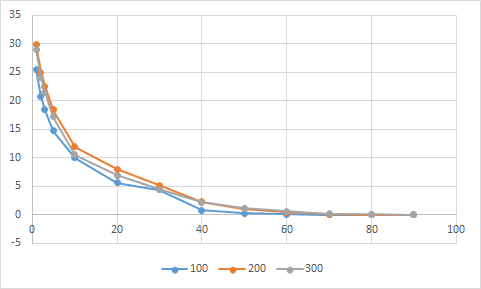
\includegraphics[scale=1]{imagenes/Experimental/DiferenciasGACEP_GRASP.png}
        \caption{Gráfica asociada a la tabla \ref{DiferenciasGACEP_GRASP}}
        \label{fig:DiferenciasGACEP}
\end{figure}

Comparando las tablas de diferencias \ref{DiferenciasGACEPv1} y \ref{DiferenciasGACEP_GRASP} se puede ver que al principio parece que sí introduce algo más de diversidad (ya que las soluciones en dichas \textit{milestones} son más diferentes a la final), aunque esto es solo notable para los tamaños $n=200$ y $n=300$. 

\section{Operador de Cruce Intensivo}

La siguiente idea a seguir tiene que ver de nuevo con la explotación de las características de las mejores soluciones. 
Anteriormente se propuso introducir una modificación para mejorar la explotación en el propio operador de reparación y en la mutación; en este caso, se pretende introducir este operador en el propio operador de cruce directamente. 

Esta modificación se basa en que las soluciones hijas heredarán una mayor cantidad de genes del mejor de los dos padres. 
La motivación de este cambio es la generación de nuevas soluciones muy parecidas a las buenas que ya forman parte de la población, con lo que hay una mayor probabilidad de que se sigan desarrollando las soluciones en ese ámbito. 

Para este trabajo probaremos con varios porcentajes de elementos que deben ser pertenecientes al mejor padre: 50\%, 60\%, 70\% y 80\%, para decidir cuál sería la mejor proporción. 
Téngase en cuenta que elegir el 50\% de los genes del mejor padre no tiene por qué tener el mismo resultado que el cruce uniforme que estamos actualmente realizando; ya que la primera opción permite que ambos hijos tengan genes en común (que provengan del mismo padre), mientras que para la segunda opción eso es imposible. 

Adicionalmente, consideraremos también dos posibilidades mayores: el utilizar GRASP de nuevo para este tipo de cruce o no. 
De antemano podríamos suponer que el uso del GRASP dará mejores resultados, ya que ayudará a diversificar unas soluciones hijas que serán muy parecidas entre sí en tanto que tomarán bastantes elementos del mismo padre. 
Pero esto debemos comprobarlo empíricamente, por ello, se calculan todos los resultados posibles y se comparan entre sí para determinar cuál es la mejor opción, la cual compararemos posteriormente con nuestro GACEPv2. 

\subsection{Utilizando GRASP}

La lógica de utilizar GRASP para el cruce intensivo es la misma que para el cruce uniforme, la utilizaremos en el operador de reparación tras generar los hijos resultantes de dicho cruce. 

Estas versiones recibirán el nombre ``\textbf{GACEPv3c\texttt{x}}'', donde \texttt{x} en este caso representaría el porcentaje de elementos que toma del mejor padre.

Dicho esto, podemos ver en la gráfica \ref{fig:GACEPcGRASP} el \textit{ranking} de los distintos porcentajes asociados al operador de cruce.

\begin{figure}[h]
     \centering
     \begin{subfigure}[b]{0.45\textwidth}
         \centering
         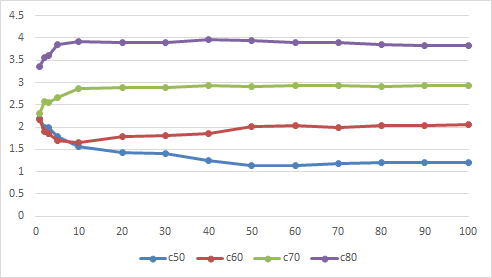
\includegraphics[width=\textwidth]{imagenes/Experimental/GACEPcGRASP.png}
         \caption{Ranking durante todas las \textit{milestones}}
         \label{fig:GACEPv3cGRASP_lineas}
     \end{subfigure}
     \hfill
     \begin{subfigure}[b]{0.45\textwidth}
         \centering
         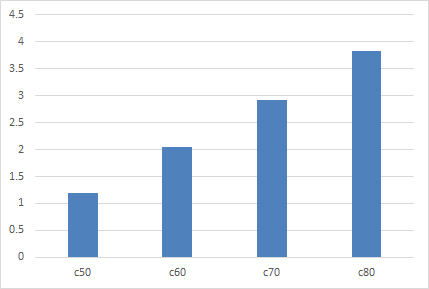
\includegraphics[width=\textwidth]{imagenes/Experimental/barras/GACEPcGRASP.png}
         \caption{Ranking final}
         \label{fig:GACEPv3cGRASP_barras}
     \end{subfigure}
        \caption{Comparación de los resultados de los GACEPv3c\texttt{x}}
        \label{fig:GACEPcGRASP}
\end{figure}

\subsection{Sin utilizar GRASP}

En este caso se seguiría usando el Operador de Reparación original (\ref{alg:OR}), donde se elige automáticamente el mejor elemento posible para introducir y el peor elemento posible para eliminar.

Estas versiones recibirán el nombre ``\textbf{GACEPv3c\texttt{x}wo}'', donde \texttt{x} en este caso representaría el porcentaje de elementos que toma del mejor padre y ``wo'' indica que no se está utilizando GRASP (\textit{without GRASP}).

En la gráfica \ref{fig:GACEPcwoGRASP} podemos apreciar el \textit{ranking} de los distintos porcentajes asociados al operador de cruce.

\begin{figure}[h]
     \centering
     \begin{subfigure}[b]{0.45\textwidth}
         \centering
         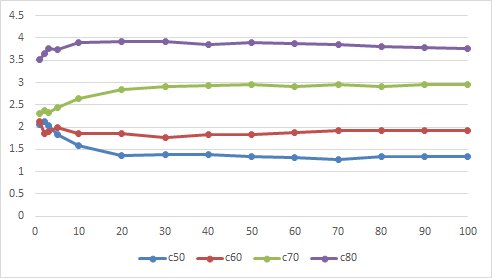
\includegraphics[width=\textwidth]{imagenes/Experimental/GACEPcwoGRASP.png}
         \caption{Ranking durante todas las \textit{milestones}}
         \label{fig:GACEPv3cwo_lineas}
     \end{subfigure}
     \hfill
     \begin{subfigure}[b]{0.45\textwidth}
         \centering
         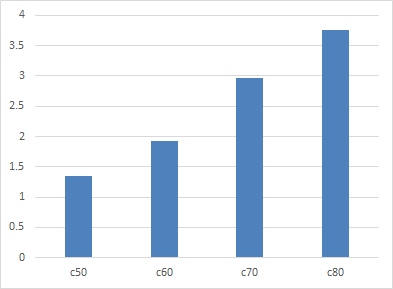
\includegraphics[width=\textwidth]{imagenes/Experimental/barras/GACEPcwoGRASP.png}
         \caption{Ranking final}
         \label{fig:GACEPv3cwo_barras}
     \end{subfigure}
        \caption{Comparación de los resultados de los GACEPv3c\texttt{x}wo}
        \label{fig:GACEPcwoGRASP}
\end{figure}

Se puede apreciar que en ambos casos, el comportamiento que tienen los algoritmos es similar, cuanto mayor sea la intensidad con la que se aplique el nuevo operador de cruce peores son los resultados. 
Con esto se puede empezar a intuir que, al menos para poblaciones pequeñas, tener muchas soluciones parecidas resulta contraproducente, ya que reduce la diversidad y llega a estancar a la población. 
Por lo tanto, procederemos a comparar las mejores versiones de ambas opciones: las dos utilizando un 50\% de los elementos del mejor padre. 
En la gráfica \ref{fig:GACEPv3c} podemos apreciar el \textit{ranking} de ambas opciones tanto para las distintas \textit{milestones} como la final sola.

\begin{figure}[h]
     \centering
     \begin{subfigure}[b]{0.45\textwidth}
         \centering
         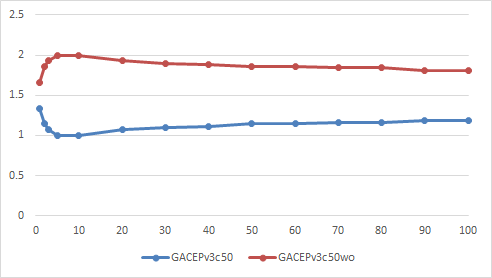
\includegraphics[width=\textwidth]{imagenes/Experimental/GACEPv3c.png}
         \caption{Ranking durante todas las \textit{milestones}}
         \label{fig:GACEPv3c_lineas}
     \end{subfigure}
     \hfill
     \begin{subfigure}[b]{0.45\textwidth}
         \centering
         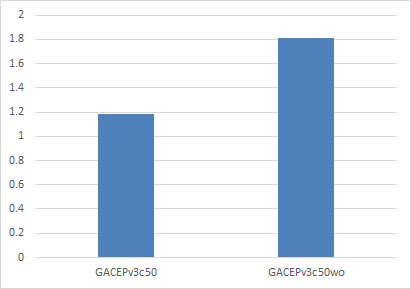
\includegraphics[width=\textwidth]{imagenes/Experimental/barras/GACEPv3c.png}
         \caption{Ranking final}
         \label{fig:GACEPv3c_barras}
     \end{subfigure}
        \caption{Comparación de los resultados de los GACEPv3c50 y GACEPv3c50wo}
        \label{fig:GACEPv3c}
\end{figure}

En \ref{fig:GACEPv3c_lineas} podemos ver que el usar la opción con GRASP es superior a la versión que no lo usa. 
Con esto podemos extraer que el uso del GRASP es adecuado para ambos operadores de cruce: el uniforme \ref{alg:CU} y el porcentual \ref{alg:CI}. 

Esto último nos lleva a tener que comparar los algoritmos GACEPv2 y GACEPv3c50 para determinar si se ha producido alguna mejora. 
Esta comparación puede ser visualizada en la gráfica \ref{fig:GACEPv2vsGACEPv3}.

\begin{figure}[h]
     \centering
     \begin{subfigure}[b]{0.45\textwidth}
         \centering
         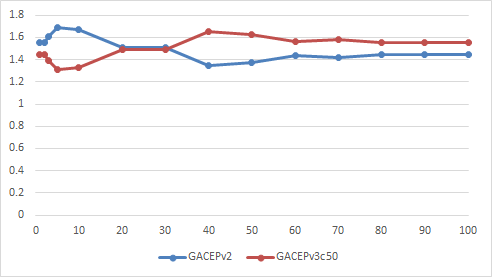
\includegraphics[width=\textwidth]{imagenes/Experimental/GACEPv2vsGACEPv3.png}
         \caption{Ranking durante todas las \textit{milestones}}
         \label{fig:GACEPv2vsGACEPv3_lineas}
     \end{subfigure}
     \hfill
     \begin{subfigure}[b]{0.45\textwidth}
         \centering
         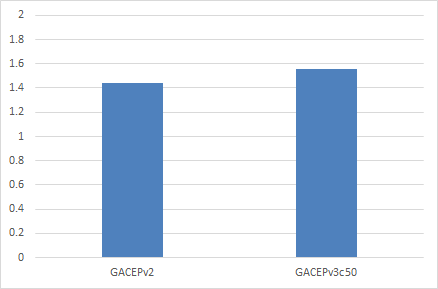
\includegraphics[width=\textwidth]{imagenes/Experimental/barras/GACEPv2vsGACEPv3.png}
         \caption{Ranking final}
         \label{fig:GACEPv2vsGACEPv3_barras}
     \end{subfigure}
        \caption{Comparación de los resultados de los GACEPv2 y GACEPv3c50}
        \label{fig:GACEPv2vsGACEPv3}
\end{figure}

En la gráfica \ref{fig:GACEPv2vsGACEPv3_lineas} que aunque en las primeras iteraciones el GACEPv3c50 tiene mejores resultados que GACEPv2, esta diferencia se reduce rápidamente. 
De hecho, las dos versiones tienen resultados muy parecidos, lo cual tiene sentido ya que el cruce uniforme y el cruce porcentual del 50\% son muy similares, aunque no iguales. 
De cualquier forma, a partir del 30\% de las iteraciones GACEPv2 obtiene mejores resultados que GACEPv3c50, aunque sea por poco. 
Por lo tanto, ignoraremos esta tercera versión y seguiremos trabajando con la segunda versión como base. 

\section{Modificaciones sobre CHC}

Llegados a este punto podemos considerar haber hecho algunos avances significativos sobre el AGEU y es momento de preguntarse si estas modificaciones se podrían aplicar al algoritmo CHC. 
Recordemos que en \ref{fig:AGEUvsCHC_lineas} podíamos apreciar que CHC obtenía mejores resultados en la primera mitad de las iteraciones y al final resultaba peor dado a que convergía prematuramente. 
Por lo tanto, en esta sección vamos a comprobar si aplicando los mismos cambios que al AGEU se logra mejorar los resultados del GACEP. 

En tanto que no es una versión puramente de GACEP, cambiaremos su notación a ``\textbf{GACEPCHCv\texttt{x}}'', donde \texttt{x} representa el número de la versión. 

\subsection{Incorporación del histórico}

El uso del histórico \ref{alg:Historico_Estructura} para CHC sigue la misma lógica que para el AGEU: el aumento de la explotación de los mejores resultados. 
Si bien a simple vista se podría pensar que el uso del histórico no debería mejorar los resultados ya que nuestro problema principal es que la población converge rápidamente a una solución se debe recordar cómo se clasificaban los distintos elementos:
\begin{itemize}
	\item \texttt{Mejores}: Aquellos elementos que suelen estar presentes en las mejores soluciones, pero no en las peores.
	\item \texttt{Peores}: Aquellos elementos que suelen estar presentes en las peores soluciones, pero no en las mejores. 
	\item \texttt{Sin información}: Aquellos elementos que frecuentemente no aparecen en las mejores ni en las peores soluciones o que aparecen en ambas (por lo que no nos aporta ninguna información ya que no se puede considerar un elemento determinista en lo buena que es una solución).
\end{itemize}
Por lo que si todas las soluciones son muy parecidas entre sí, teniendo todas el mismo conjunto de elementos, estos elementos no se considerarán ``mejores'' que el resto y tendrán la misma probabilidad de ser elegidas que el resto de elementos que no se han explorado anteriormente. 

Esta versión se denominará \textbf{GACEPCHCv1}.

Como hemos hecho previamente, obtendremos sus resultados, los cuales están almacenados en \color{red} METER TABLA EN EL APENDICE\color{black}. 
Estos resultados los compararemos con los del CHC versión \textit{expensive} para determinar si se ha producido algún tipo de mejora. 
Esta comparación será visible en la gráfica \ref{fig:CHCvsGACEPCHCv1}

\begin{figure}[h]
     \centering
     \begin{subfigure}[b]{0.45\textwidth}
         \centering
         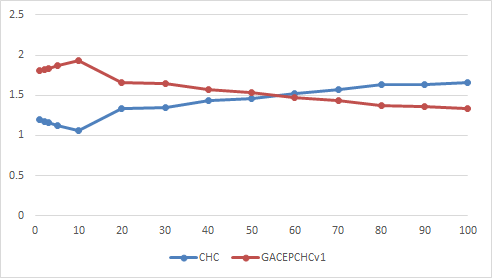
\includegraphics[width=\textwidth]{imagenes/Experimental/CHCvsGACEPCHCv1.png}
         \caption{Ranking durante todas las \textit{milestones}}
         \label{fig:CHCvsGACEPCHCv1_lineas}
     \end{subfigure}
     \hfill
     \begin{subfigure}[b]{0.45\textwidth}
         \centering
         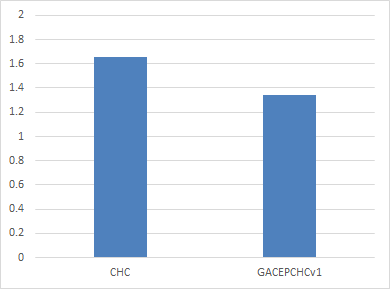
\includegraphics[width=\textwidth]{imagenes/Experimental/barras/CHCvsGACEPCHCv1.png}
         \caption{Ranking final}
         \label{fig:CHCvsGACEPCHCv1_barras}
     \end{subfigure}
        \caption{Comparación de los resultados de CHC y GACEPCHCv1}
        \label{fig:CHCvsGACEPCHCv1}
\end{figure}

En esta gráfica \ref{fig:CHCvsGACEPCHCv1} se puede apreciar que aunque inicialmente GACEPCHCv1 es bastante peor que CHC, tras la mitad de las ejecuciones logra mejorarlo. 
Esto podría estar causado por el hecho de que CHC converge rápidamente antes de la mitad de las ejecuciones y que GACEPCHCv1 puede que siga mejorando poco a poco como lo harían las versiones anteriores basadas en AGEU debido a cierto aumento de la diversidad en la población. 
Para comprobar si este es el caso, estudiaremos las diferencias entre las soluciones de las distintas \textit{milestones} y la final. 
Esta información se mostrará en la tabla y su correspondiente gráfica

%GACEPCHCv1
\begin{table}[]
\begin{tabular}{|ccrccrccr|}
\hline
\rowcolor[HTML]{FFFFC7} 
\multicolumn{9}{|c|}{\cellcolor[HTML]{FFFFC7}GACEPCHCv1}                                                                                                                                                                                                                                                                                                                                                                                                                                                                                                                                             \\ \hline
\rowcolor[HTML]{F7EAC7} 
\multicolumn{1}{|c|}{\cellcolor[HTML]{F7EAC7}n}                               & \multicolumn{1}{c|}{\cellcolor[HTML]{F7EAC7}milestone} & \multicolumn{1}{l|}{\cellcolor[HTML]{F7EAC7}Diferencia} & \multicolumn{1}{c|}{\cellcolor[HTML]{F7EAC7}n}                               & \multicolumn{1}{c|}{\cellcolor[HTML]{F7EAC7}milestone} & \multicolumn{1}{l|}{\cellcolor[HTML]{F7EAC7}Diferencia} & \multicolumn{1}{c|}{\cellcolor[HTML]{F7EAC7}n}                               & \multicolumn{1}{c|}{\cellcolor[HTML]{F7EAC7}milestone} & \multicolumn{1}{l|}{\cellcolor[HTML]{F7EAC7}Diferencia} \\ \hline
\rowcolor[HTML]{DAE8FC} 
\multicolumn{1}{|c|}{\cellcolor[HTML]{FFFFC7}}                                & \multicolumn{1}{c|}{\cellcolor[HTML]{DAE8FC}1}         & \multicolumn{1}{r|}{\cellcolor[HTML]{DAE8FC}26.7201}    & \multicolumn{1}{c|}{\cellcolor[HTML]{FFFFC7}}                                & \multicolumn{1}{c|}{\cellcolor[HTML]{DAE8FC}1}         & \multicolumn{1}{r|}{\cellcolor[HTML]{DAE8FC}25.7172359} & \multicolumn{1}{c|}{\cellcolor[HTML]{FFFFC7}}                                & \multicolumn{1}{c|}{\cellcolor[HTML]{DAE8FC}1}         & 26.2254573                                              \\ \cline{2-3} \cline{5-6} \cline{8-9} 
\rowcolor[HTML]{DDFDFF} 
\multicolumn{1}{|c|}{\cellcolor[HTML]{FFFFC7}}                                & \multicolumn{1}{c|}{\cellcolor[HTML]{DDFDFF}2}         & \multicolumn{1}{r|}{\cellcolor[HTML]{DDFDFF}23.2096}    & \multicolumn{1}{c|}{\cellcolor[HTML]{FFFFC7}}                                & \multicolumn{1}{c|}{\cellcolor[HTML]{DDFDFF}2}         & \multicolumn{1}{r|}{\cellcolor[HTML]{DDFDFF}22.3721298} & \multicolumn{1}{c|}{\cellcolor[HTML]{FFFFC7}}                                & \multicolumn{1}{c|}{\cellcolor[HTML]{DDFDFF}2}         & 22.0835516                                              \\ \cline{2-3} \cline{5-6} \cline{8-9} 
\rowcolor[HTML]{DAE8FC} 
\multicolumn{1}{|c|}{\cellcolor[HTML]{FFFFC7}}                                & \multicolumn{1}{c|}{\cellcolor[HTML]{DAE8FC}3}         & \multicolumn{1}{r|}{\cellcolor[HTML]{DAE8FC}21.5554}    & \multicolumn{1}{c|}{\cellcolor[HTML]{FFFFC7}}                                & \multicolumn{1}{c|}{\cellcolor[HTML]{DAE8FC}3}         & \multicolumn{1}{r|}{\cellcolor[HTML]{DAE8FC}20.5934122} & \multicolumn{1}{c|}{\cellcolor[HTML]{FFFFC7}}                                & \multicolumn{1}{c|}{\cellcolor[HTML]{DAE8FC}3}         & 20.2131967                                              \\ \cline{2-3} \cline{5-6} \cline{8-9} 
\rowcolor[HTML]{DDFDFF} 
\multicolumn{1}{|c|}{\cellcolor[HTML]{FFFFC7}}                                & \multicolumn{1}{c|}{\cellcolor[HTML]{DDFDFF}5}         & \multicolumn{1}{r|}{\cellcolor[HTML]{DDFDFF}18.774}     & \multicolumn{1}{c|}{\cellcolor[HTML]{FFFFC7}}                                & \multicolumn{1}{c|}{\cellcolor[HTML]{DDFDFF}5}         & \multicolumn{1}{r|}{\cellcolor[HTML]{DDFDFF}17.9674193} & \multicolumn{1}{c|}{\cellcolor[HTML]{FFFFC7}}                                & \multicolumn{1}{c|}{\cellcolor[HTML]{DDFDFF}5}         & 17.375892                                               \\ \cline{2-3} \cline{5-6} \cline{8-9} 
\rowcolor[HTML]{DAE8FC} 
\multicolumn{1}{|c|}{\cellcolor[HTML]{FFFFC7}}                                & \multicolumn{1}{c|}{\cellcolor[HTML]{DAE8FC}10}        & \multicolumn{1}{r|}{\cellcolor[HTML]{DAE8FC}14.7039}    & \multicolumn{1}{c|}{\cellcolor[HTML]{FFFFC7}}                                & \multicolumn{1}{c|}{\cellcolor[HTML]{DAE8FC}10}        & \multicolumn{1}{r|}{\cellcolor[HTML]{DAE8FC}13.6488991} & \multicolumn{1}{c|}{\cellcolor[HTML]{FFFFC7}}                                & \multicolumn{1}{c|}{\cellcolor[HTML]{DAE8FC}10}        & 12.7586834                                              \\ \cline{2-3} \cline{5-6} \cline{8-9} 
\rowcolor[HTML]{DDFDFF} 
\multicolumn{1}{|c|}{\cellcolor[HTML]{FFFFC7}}                                & \multicolumn{1}{c|}{\cellcolor[HTML]{DDFDFF}20}        & \multicolumn{1}{r|}{\cellcolor[HTML]{DDFDFF}5.48547}    & \multicolumn{1}{c|}{\cellcolor[HTML]{FFFFC7}}                                & \multicolumn{1}{c|}{\cellcolor[HTML]{DDFDFF}20}        & \multicolumn{1}{r|}{\cellcolor[HTML]{DDFDFF}4.77580753} & \multicolumn{1}{c|}{\cellcolor[HTML]{FFFFC7}}                                & \multicolumn{1}{c|}{\cellcolor[HTML]{DDFDFF}20}        & 4.55863648                                              \\ \cline{2-3} \cline{5-6} \cline{8-9} 
\rowcolor[HTML]{DAE8FC} 
\multicolumn{1}{|c|}{\cellcolor[HTML]{FFFFC7}}                                & \multicolumn{1}{c|}{\cellcolor[HTML]{DAE8FC}30}        & \multicolumn{1}{r|}{\cellcolor[HTML]{DAE8FC}4.59547}    & \multicolumn{1}{c|}{\cellcolor[HTML]{FFFFC7}}                                & \multicolumn{1}{c|}{\cellcolor[HTML]{DAE8FC}30}        & \multicolumn{1}{r|}{\cellcolor[HTML]{DAE8FC}4.01781911} & \multicolumn{1}{c|}{\cellcolor[HTML]{FFFFC7}}                                & \multicolumn{1}{c|}{\cellcolor[HTML]{DAE8FC}30}        & 3.702351                                                \\ \cline{2-3} \cline{5-6} \cline{8-9} 
\rowcolor[HTML]{DDFDFF} 
\multicolumn{1}{|c|}{\cellcolor[HTML]{FFFFC7}}                                & \multicolumn{1}{c|}{\cellcolor[HTML]{DDFDFF}40}        & \multicolumn{1}{r|}{\cellcolor[HTML]{DDFDFF}2.47563}    & \multicolumn{1}{c|}{\cellcolor[HTML]{FFFFC7}}                                & \multicolumn{1}{c|}{\cellcolor[HTML]{DDFDFF}40}        & \multicolumn{1}{r|}{\cellcolor[HTML]{DDFDFF}2.54730194} & \multicolumn{1}{c|}{\cellcolor[HTML]{FFFFC7}}                                & \multicolumn{1}{c|}{\cellcolor[HTML]{DDFDFF}40}        & 2.39425407                                              \\ \cline{2-3} \cline{5-6} \cline{8-9} 
\rowcolor[HTML]{DAE8FC} 
\multicolumn{1}{|c|}{\cellcolor[HTML]{FFFFC7}}                                & \multicolumn{1}{c|}{\cellcolor[HTML]{DAE8FC}50}        & \multicolumn{1}{r|}{\cellcolor[HTML]{DAE8FC}1.75038}    & \multicolumn{1}{c|}{\cellcolor[HTML]{FFFFC7}}                                & \multicolumn{1}{c|}{\cellcolor[HTML]{DAE8FC}50}        & \multicolumn{1}{r|}{\cellcolor[HTML]{DAE8FC}1.97120082} & \multicolumn{1}{c|}{\cellcolor[HTML]{FFFFC7}}                                & \multicolumn{1}{c|}{\cellcolor[HTML]{DAE8FC}50}        & 1.90218522                                              \\ \cline{2-3} \cline{5-6} \cline{8-9} 
\rowcolor[HTML]{DDFDFF} 
\multicolumn{1}{|c|}{\cellcolor[HTML]{FFFFC7}}                                & \multicolumn{1}{c|}{\cellcolor[HTML]{DDFDFF}60}        & \multicolumn{1}{r|}{\cellcolor[HTML]{DDFDFF}1.14161}    & \multicolumn{1}{c|}{\cellcolor[HTML]{FFFFC7}}                                & \multicolumn{1}{c|}{\cellcolor[HTML]{DDFDFF}60}        & \multicolumn{1}{r|}{\cellcolor[HTML]{DDFDFF}1.35810173} & \multicolumn{1}{c|}{\cellcolor[HTML]{FFFFC7}}                                & \multicolumn{1}{c|}{\cellcolor[HTML]{DDFDFF}60}        & 1.29008322                                              \\ \cline{2-3} \cline{5-6} \cline{8-9} 
\rowcolor[HTML]{DAE8FC} 
\multicolumn{1}{|c|}{\cellcolor[HTML]{FFFFC7}}                                & \multicolumn{1}{c|}{\cellcolor[HTML]{DAE8FC}70}        & \multicolumn{1}{r|}{\cellcolor[HTML]{DAE8FC}0.62625}    & \multicolumn{1}{c|}{\cellcolor[HTML]{FFFFC7}}                                & \multicolumn{1}{c|}{\cellcolor[HTML]{DAE8FC}70}        & \multicolumn{1}{r|}{\cellcolor[HTML]{DAE8FC}0.82009965} & \multicolumn{1}{c|}{\cellcolor[HTML]{FFFFC7}}                                & \multicolumn{1}{c|}{\cellcolor[HTML]{DAE8FC}70}        & 0.81355995                                              \\ \cline{2-3} \cline{5-6} \cline{8-9} 
\rowcolor[HTML]{DDFDFF} 
\multicolumn{1}{|c|}{\cellcolor[HTML]{FFFFC7}}                                & \multicolumn{1}{c|}{\cellcolor[HTML]{DDFDFF}80}        & \multicolumn{1}{r|}{\cellcolor[HTML]{DDFDFF}0.44086}    & \multicolumn{1}{c|}{\cellcolor[HTML]{FFFFC7}}                                & \multicolumn{1}{c|}{\cellcolor[HTML]{DDFDFF}80}        & \multicolumn{1}{r|}{\cellcolor[HTML]{DDFDFF}0.55229199} & \multicolumn{1}{c|}{\cellcolor[HTML]{FFFFC7}}                                & \multicolumn{1}{c|}{\cellcolor[HTML]{DDFDFF}80}        & 0.54620318                                              \\ \cline{2-3} \cline{5-6} \cline{8-9} 
\rowcolor[HTML]{DAE8FC} 
\multicolumn{1}{|c|}{\multirow{-13}{*}{\cellcolor[HTML]{FFFFC7}\textbf{100}}} & \multicolumn{1}{c|}{\cellcolor[HTML]{DAE8FC}90}        & \multicolumn{1}{r|}{\cellcolor[HTML]{DAE8FC}0.00726}    & \multicolumn{1}{c|}{\multirow{-13}{*}{\cellcolor[HTML]{FFFFC7}\textbf{200}}} & \multicolumn{1}{c|}{\cellcolor[HTML]{DAE8FC}90}        & \multicolumn{1}{r|}{\cellcolor[HTML]{DAE8FC}0.01307933} & \multicolumn{1}{c|}{\multirow{-13}{*}{\cellcolor[HTML]{FFFFC7}\textbf{300}}} & \multicolumn{1}{c|}{\cellcolor[HTML]{DAE8FC}90}        & 0.03623624                                              \\ \hline
\end{tabular}
\caption{\label{DiferenciasGACEPCHCv1}Diferencias de los resultados de las distintas milestones con respecto a la final para el algoritmo GACEPCHCv1}
\end{table}

\begin{figure}[h]
		\centering
		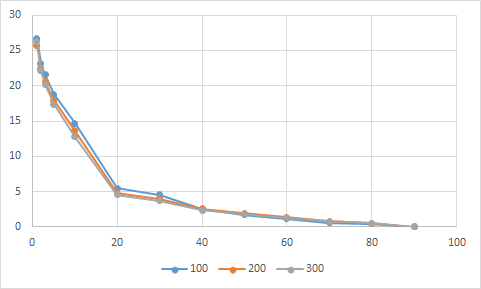
\includegraphics[scale=1]{imagenes/Experimental/DiferenciasGACEPCHCv1.png}
        \caption{Gráfica asociada a la tabla \ref{DiferenciasGACEPCHCv1}}
        \label{fig:DiferenciasGACEPCHCv1}
\end{figure}

Efectivamente, en la gráfica \ref{fig:DiferenciasGACEPCHCv1} se puede comprobar visualmente que tiene un comportamiento parecido al de las versiones de AGEU, aunque bien es verdad que es bastante más abrupto.

\subsection{Uso del GRASP}

Nuestro objetivo sigue siendo aumentar la exploración del algoritmo para conseguir una población aún más diversa y que las soluciones no converjan de forma prematura. 
Por ello se considera que este algoritmo se podría beneficiar en gran medida del uso del GRASP, podremos mantener la diversidad de la población a lo largo de la ejecución del algoritmo y, a la vez, se garantiza que las soluciones seguirán siendo competentes. 

Esta nueva versión está construida usando GACEPCHCv1 de base y la denominaremos \textbf{GACEPCHCv2}.

Tras su implementación, debemos recoger sus resultados, los cuales están almacenados en la tabla \color{red}METER TABLA EN EL APENDICE\color{black}. 
Tras esto, en primer lugar compararemos GACEPCHCv1 y GACEPCHCv2 para comprobar que realmente se ha producido una mejora de los resultados con respecto a la versión anterior. 
Esta comparación será visible en la gráfica \ref{fig:GACEPCHCv1vsGACEPCHCv2}.

\begin{figure}[h]
     \centering
     \begin{subfigure}[b]{0.45\textwidth}
         \centering
         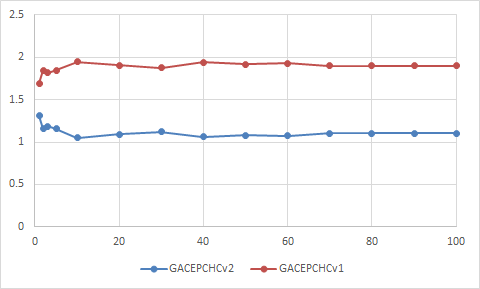
\includegraphics[width=\textwidth]{imagenes/Experimental/GACEPCHCv1vsGACEPCHCv2.png}
         \caption{Ranking durante todas las \textit{milestones}}
         \label{fig:GACEPCHCv1vsGACEPCHCv2_lineas}
     \end{subfigure}
     \hfill
     \begin{subfigure}[b]{0.45\textwidth}
         \centering
         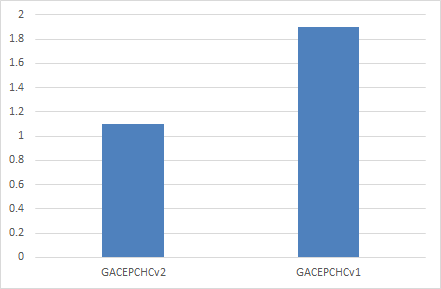
\includegraphics[width=\textwidth]{imagenes/Experimental/barras/GACEPCHCv1vsGACEPCHCv2.png}
         \caption{Ranking final}
         \label{fig:GACEPCHCv1vsGACEPCHCv2_barras}
     \end{subfigure}
        \caption{Comparación de los resultados de GACEPCHCv1 y GACEPCHCv2}
        \label{fig:GACEPCHCv1vsGACEPCHCv2}
\end{figure}

En esta gráfica \ref{fig:GACEPCHCv1vsGACEPCHCv2} podemos comprobar que efectivamente se produce una mejora con respecto a la versión anterior. 
Por lo que podemos proceder a realizar una comparación con la versión equivalente para el algoritmo AGEU: GACEPv2. 
Esta comparación será visible en la gráfica \ref{fig:GACEPv2vsGACEPCHCv2}.

\begin{figure}[h]
     \centering
     \begin{subfigure}[b]{0.45\textwidth}
         \centering
         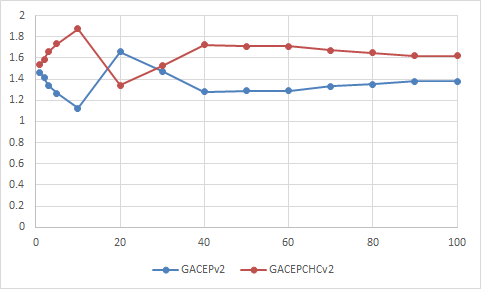
\includegraphics[width=\textwidth]{imagenes/Experimental/GACEPv2vsGACEPCHCv2.png}
         \caption{Ranking durante todas las \textit{milestones}}
         \label{fig:GACEPv2vsGACEPCHCv2_lineas}
     \end{subfigure}
     \hfill
     \begin{subfigure}[b]{0.45\textwidth}
         \centering
         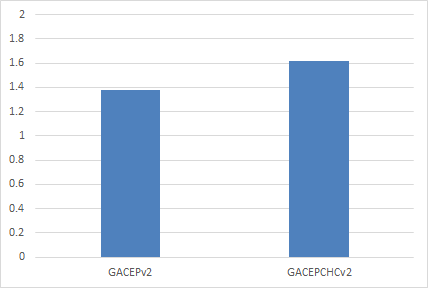
\includegraphics[width=\textwidth]{imagenes/Experimental/barras/GACEPv2vsGACEPCHCv2.png}
         \caption{Ranking final}
         \label{fig:GACEPv2vsGACEPCHCv2_barras}
     \end{subfigure}
        \caption{Comparación de los resultados de GACEPv2 y GACEPCHCv2}
        \label{fig:GACEPv2vsGACEPCHCv2}
\end{figure}

En la gráfica \ref{fig:GACEPv2vsGACEPCHCv2} se puede ver cómo GACEPv2 obtiene mejores resultados que GACEPCHCv2 en la mayoría de las \textit{milestones}, sobre todo y más importante, obtiene mejores resultados finales. 
En tanto que no se ha logrado mejorar los resultados de una versión anterior, descartaremos estos cambios y seguiremos trabajando exclusivamente sobre el algoritmo GACEPv2.

\section{Estudio de la diversidad}

Durante este capítulo hemos asociado la abrupta convergencia a una solución como falta de diversidad en la población. 
Para comprobar esto, se ha decidido utilizar la fórmula para el cálculo de la diversidad propuesta en \parencite{oppacherShiftingBalanceGenetic}, donde se tiene que:
\begin{equation}
\text{Diversidad}(P) = \dfrac{1}{n\cdot \texttt{numcro}(\texttt{numcro}-1)}\sum_{i=1}^{\texttt{numcro}}\sum_{j=1}^{\texttt{numcro}} HD(p_i,p_j)
\label{eq:Diversidad}
\end{equation}
donde $P$ es la población, $n$ es la longitud del individuo, $HD$ es la función de la distancia de Hamming y $p_i$ es el individuo $i$-ésimo de la población $P$.

Se han almacenado en la Tabla \ref{GACEPv2Diversity} los resultados de aplicar la fórmula \ref{eq:Diversidad} a la población que hemos conseguido en cada \textit{milestone}

\begin{table}[h]
\begin{tabular}{|cclcclccl|}
\hline
\rowcolor[HTML]{FFFFC7} 
\multicolumn{9}{|c|}{\cellcolor[HTML]{FFFFC7}GACEPv2}                                                                                                                                                                                                                                                                                                                                                                                                                                                                                                      \\ \hline
\rowcolor[HTML]{FCE6AB} 
\multicolumn{1}{|c|}{\cellcolor[HTML]{FCE6AB}n}                               & \multicolumn{1}{c|}{\cellcolor[HTML]{FCE6AB}milestone} & \multicolumn{1}{l|}{\cellcolor[HTML]{FCE6AB}Diversidad}  & \multicolumn{1}{c|}{\cellcolor[HTML]{FCE6AB}n}                               & \multicolumn{1}{c|}{\cellcolor[HTML]{FCE6AB}milestone} & \multicolumn{1}{l|}{\cellcolor[HTML]{FCE6AB}Diversidad}  & \multicolumn{1}{c|}{\cellcolor[HTML]{FCE6AB}n}                               & \multicolumn{1}{c|}{\cellcolor[HTML]{FCE6AB}milestone} & Diversidad  \\ \hline
\rowcolor[HTML]{DAE8FC} 
\multicolumn{1}{|c|}{\cellcolor[HTML]{FFFFC7}}                                & \multicolumn{1}{c|}{\cellcolor[HTML]{DAE8FC}1}         & \multicolumn{1}{l|}{\cellcolor[HTML]{DAE8FC}0.295980449} & \multicolumn{1}{c|}{\cellcolor[HTML]{FFFFC7}}                                & \multicolumn{1}{c|}{\cellcolor[HTML]{DAE8FC}1}         & \multicolumn{1}{l|}{\cellcolor[HTML]{DAE8FC}0.303604262} & \multicolumn{1}{c|}{\cellcolor[HTML]{FFFFC7}}                                & \multicolumn{1}{c|}{\cellcolor[HTML]{DAE8FC}1}         & 0.285172532 \\ \cline{2-3} \cline{5-6} \cline{8-9} 
\rowcolor[HTML]{DDFDFF} 
\multicolumn{1}{|c|}{\cellcolor[HTML]{FFFFC7}}                                & \multicolumn{1}{c|}{\cellcolor[HTML]{DDFDFF}2}         & \multicolumn{1}{l|}{\cellcolor[HTML]{DDFDFF}0.239986795} & \multicolumn{1}{c|}{\cellcolor[HTML]{FFFFC7}}                                & \multicolumn{1}{c|}{\cellcolor[HTML]{DDFDFF}2}         & \multicolumn{1}{l|}{\cellcolor[HTML]{DDFDFF}0.236957486} & \multicolumn{1}{c|}{\cellcolor[HTML]{FFFFC7}}                                & \multicolumn{1}{c|}{\cellcolor[HTML]{DDFDFF}2}         & 0.228452411 \\ \cline{2-3} \cline{5-6} \cline{8-9} 
\rowcolor[HTML]{DAE8FC} 
\multicolumn{1}{|c|}{\cellcolor[HTML]{FFFFC7}}                                & \multicolumn{1}{c|}{\cellcolor[HTML]{DAE8FC}3}         & \multicolumn{1}{l|}{\cellcolor[HTML]{DAE8FC}0.20074531}  & \multicolumn{1}{c|}{\cellcolor[HTML]{FFFFC7}}                                & \multicolumn{1}{c|}{\cellcolor[HTML]{DAE8FC}3}         & \multicolumn{1}{l|}{\cellcolor[HTML]{DAE8FC}0.196295669} & \multicolumn{1}{c|}{\cellcolor[HTML]{FFFFC7}}                                & \multicolumn{1}{c|}{\cellcolor[HTML]{DAE8FC}3}         & 0.1877086   \\ \cline{2-3} \cline{5-6} \cline{8-9} 
\rowcolor[HTML]{DDFDFF} 
\multicolumn{1}{|c|}{\cellcolor[HTML]{FFFFC7}}                                & \multicolumn{1}{c|}{\cellcolor[HTML]{DDFDFF}5}         & \multicolumn{1}{l|}{\cellcolor[HTML]{DDFDFF}0.136337387} & \multicolumn{1}{c|}{\cellcolor[HTML]{FFFFC7}}                                & \multicolumn{1}{c|}{\cellcolor[HTML]{DDFDFF}5}         & \multicolumn{1}{l|}{\cellcolor[HTML]{DDFDFF}0.127482734} & \multicolumn{1}{c|}{\cellcolor[HTML]{FFFFC7}}                                & \multicolumn{1}{c|}{\cellcolor[HTML]{DDFDFF}5}         & 0.1235785   \\ \cline{2-3} \cline{5-6} \cline{8-9} 
\rowcolor[HTML]{DAE8FC} 
\multicolumn{1}{|c|}{\cellcolor[HTML]{FFFFC7}}                                & \multicolumn{1}{c|}{\cellcolor[HTML]{DAE8FC}10}        & \multicolumn{1}{l|}{\cellcolor[HTML]{DAE8FC}0.068669744} & \multicolumn{1}{c|}{\cellcolor[HTML]{FFFFC7}}                                & \multicolumn{1}{c|}{\cellcolor[HTML]{DAE8FC}10}        & \multicolumn{1}{l|}{\cellcolor[HTML]{DAE8FC}0.056736476} & \multicolumn{1}{c|}{\cellcolor[HTML]{FFFFC7}}                                & \multicolumn{1}{c|}{\cellcolor[HTML]{DAE8FC}10}        & 0.051865263 \\ \cline{2-3} \cline{5-6} \cline{8-9} 
\rowcolor[HTML]{DDFDFF} 
\multicolumn{1}{|c|}{\cellcolor[HTML]{FFFFC7}}                                & \multicolumn{1}{c|}{\cellcolor[HTML]{DDFDFF}20}        & \multicolumn{1}{l|}{\cellcolor[HTML]{DDFDFF}0.034505642} & \multicolumn{1}{c|}{\cellcolor[HTML]{FFFFC7}}                                & \multicolumn{1}{c|}{\cellcolor[HTML]{DDFDFF}20}        & \multicolumn{1}{l|}{\cellcolor[HTML]{DDFDFF}0.027917386} & \multicolumn{1}{c|}{\cellcolor[HTML]{FFFFC7}}                                & \multicolumn{1}{c|}{\cellcolor[HTML]{DDFDFF}20}        & 0.020362715 \\ \cline{2-3} \cline{5-6} \cline{8-9} 
\rowcolor[HTML]{DAE8FC} 
\multicolumn{1}{|c|}{\cellcolor[HTML]{FFFFC7}}                                & \multicolumn{1}{c|}{\cellcolor[HTML]{DAE8FC}30}        & \multicolumn{1}{l|}{\cellcolor[HTML]{DAE8FC}0.028956809} & \multicolumn{1}{c|}{\cellcolor[HTML]{FFFFC7}}                                & \multicolumn{1}{c|}{\cellcolor[HTML]{DAE8FC}30}        & \multicolumn{1}{l|}{\cellcolor[HTML]{DAE8FC}0.025366897} & \multicolumn{1}{c|}{\cellcolor[HTML]{FFFFC7}}                                & \multicolumn{1}{c|}{\cellcolor[HTML]{DAE8FC}30}        & 0.018587216 \\ \cline{2-3} \cline{5-6} \cline{8-9} 
\rowcolor[HTML]{DDFDFF} 
\multicolumn{1}{|c|}{\cellcolor[HTML]{FFFFC7}}                                & \multicolumn{1}{c|}{\cellcolor[HTML]{DDFDFF}40}        & \multicolumn{1}{l|}{\cellcolor[HTML]{DDFDFF}0.017469288} & \multicolumn{1}{c|}{\cellcolor[HTML]{FFFFC7}}                                & \multicolumn{1}{c|}{\cellcolor[HTML]{DDFDFF}40}        & \multicolumn{1}{l|}{\cellcolor[HTML]{DDFDFF}0.019192113} & \multicolumn{1}{c|}{\cellcolor[HTML]{FFFFC7}}                                & \multicolumn{1}{c|}{\cellcolor[HTML]{DDFDFF}40}        & 0.01590612  \\ \cline{2-3} \cline{5-6} \cline{8-9} 
\rowcolor[HTML]{DAE8FC} 
\multicolumn{1}{|c|}{\cellcolor[HTML]{FFFFC7}}                                & \multicolumn{1}{c|}{\cellcolor[HTML]{DAE8FC}50}        & \multicolumn{1}{l|}{\cellcolor[HTML]{DAE8FC}0.011608889} & \multicolumn{1}{c|}{\cellcolor[HTML]{FFFFC7}}                                & \multicolumn{1}{c|}{\cellcolor[HTML]{DAE8FC}50}        & \multicolumn{1}{l|}{\cellcolor[HTML]{DAE8FC}0.014284978} & \multicolumn{1}{c|}{\cellcolor[HTML]{FFFFC7}}                                & \multicolumn{1}{c|}{\cellcolor[HTML]{DAE8FC}50}        & 0.013201013 \\ \cline{2-3} \cline{5-6} \cline{8-9} 
\rowcolor[HTML]{DDFDFF} 
\multicolumn{1}{|c|}{\cellcolor[HTML]{FFFFC7}}                                & \multicolumn{1}{c|}{\cellcolor[HTML]{DDFDFF}60}        & \multicolumn{1}{l|}{\cellcolor[HTML]{DDFDFF}0.0096147}   & \multicolumn{1}{c|}{\cellcolor[HTML]{FFFFC7}}                                & \multicolumn{1}{c|}{\cellcolor[HTML]{DDFDFF}60}        & \multicolumn{1}{l|}{\cellcolor[HTML]{DDFDFF}0.012227811} & \multicolumn{1}{c|}{\cellcolor[HTML]{FFFFC7}}                                & \multicolumn{1}{c|}{\cellcolor[HTML]{DDFDFF}60}        & 0.011819336 \\ \cline{2-3} \cline{5-6} \cline{8-9} 
\rowcolor[HTML]{DAE8FC} 
\multicolumn{1}{|c|}{\cellcolor[HTML]{FFFFC7}}                                & \multicolumn{1}{c|}{\cellcolor[HTML]{DAE8FC}70}        & \multicolumn{1}{l|}{\cellcolor[HTML]{DAE8FC}0.007890714} & \multicolumn{1}{c|}{\cellcolor[HTML]{FFFFC7}}                                & \multicolumn{1}{c|}{\cellcolor[HTML]{DAE8FC}70}        & \multicolumn{1}{l|}{\cellcolor[HTML]{DAE8FC}0.009880155} & \multicolumn{1}{c|}{\cellcolor[HTML]{FFFFC7}}                                & \multicolumn{1}{c|}{\cellcolor[HTML]{DAE8FC}70}        & 0.010087172 \\ \cline{2-3} \cline{5-6} \cline{8-9} 
\rowcolor[HTML]{DDFDFF} 
\multicolumn{1}{|c|}{\cellcolor[HTML]{FFFFC7}}                                & \multicolumn{1}{c|}{\cellcolor[HTML]{DDFDFF}80}        & \multicolumn{1}{l|}{\cellcolor[HTML]{DDFDFF}0.007583591} & \multicolumn{1}{c|}{\cellcolor[HTML]{FFFFC7}}                                & \multicolumn{1}{c|}{\cellcolor[HTML]{DDFDFF}80}        & \multicolumn{1}{l|}{\cellcolor[HTML]{DDFDFF}0.009224822} & \multicolumn{1}{c|}{\cellcolor[HTML]{FFFFC7}}                                & \multicolumn{1}{c|}{\cellcolor[HTML]{DDFDFF}80}        & 0.009189166 \\ \cline{2-3} \cline{5-6} \cline{8-9} 
\rowcolor[HTML]{DAE8FC} 
\multicolumn{1}{|c|}{\cellcolor[HTML]{FFFFC7}}                                & \multicolumn{1}{c|}{\cellcolor[HTML]{DAE8FC}90}        & \multicolumn{1}{l|}{\cellcolor[HTML]{DAE8FC}0.006994988} & \multicolumn{1}{c|}{\cellcolor[HTML]{FFFFC7}}                                & \multicolumn{1}{c|}{\cellcolor[HTML]{DAE8FC}90}        & \multicolumn{1}{l|}{\cellcolor[HTML]{DAE8FC}0.008364826} & \multicolumn{1}{c|}{\cellcolor[HTML]{FFFFC7}}                                & \multicolumn{1}{c|}{\cellcolor[HTML]{DAE8FC}90}        & 0.007948148 \\ \cline{2-3} \cline{5-6} \cline{8-9} 
\rowcolor[HTML]{DDFDFF} 
\multicolumn{1}{|c|}{\multirow{-14}{*}{\cellcolor[HTML]{FFFFC7}\textbf{100}}} & \multicolumn{1}{c|}{\cellcolor[HTML]{DDFDFF}100}       & \multicolumn{1}{l|}{\cellcolor[HTML]{DDFDFF}0.007128205} & \multicolumn{1}{c|}{\multirow{-14}{*}{\cellcolor[HTML]{FFFFC7}\textbf{200}}} & \multicolumn{1}{c|}{\cellcolor[HTML]{DDFDFF}100}       & \multicolumn{1}{l|}{\cellcolor[HTML]{DDFDFF}0.00819632}  & \multicolumn{1}{c|}{\multirow{-14}{*}{\cellcolor[HTML]{FFFFC7}\textbf{300}}} & \multicolumn{1}{c|}{\cellcolor[HTML]{DDFDFF}100}       & 0.007950337 \\ \hline
\end{tabular}
\caption{\label{GACEPv2Diversity}Diversidad de la población en las distintas milestones para el algoritmo GACEPv2}
\end{table}

\begin{figure}[h]
		\centering
		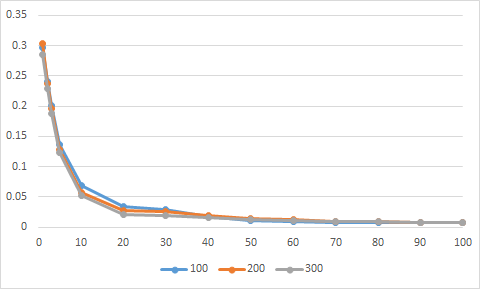
\includegraphics[scale=1]{imagenes/Experimental/GACEPv2_Diversity.png}
        \caption{Gráfica asociada a la tabla \ref{GACEPv2Diversity}}
        \label{fig:GACEPv2_Diversity}
\end{figure}

Como se puede comprobar de forma más visual en la gráfica \ref{fig:GACEPv2_Diversity}, la diversidad de la población se reduce en gran medida al llegar al 20\% de las iteraciones (se reduce a aproximadamente un 10\% de la diversidad inicial). 
Además, la diversidad en muy pocos casos aumenta, y cuando lo hace, solo aumenta una cantidad inferior a las milésimas. 
Con esto ya es claro que se pierde mucha diversidad en la población y esto se produce en las etapas iniciales de la ejecución. 

Este descubrimiento es lo que nos motiva a implementar nuevas versiones que contengan modificaciones dedicadas especialmente a introducir y/o mantener la diversidad en la población. 

\section{Incrementando la diversidad}

Con motivo del estudio realizado en la sección anterior, resulta necesario introducir modificaciones que sean capaces de introducir y/o mantener diversidad en la población. 
En este trabajo se proponen algunas modificaciones, las cuales se explicarán individualmente y qué sentido podría tener combinarlas, comparándolas con el algoritmo GACEPv2. 
Finalmente, compararemos todas las versiones de esta sección entre sí para determinar cuál es la mejor y presentaremos como la versión final de este desarrollo. 

Un resumen de las modificaciones que aplicaremos a continuación es:
\begin{itemize}
	\item Población inicial diversa \ref{alg:PD}: Nos aseguramos que la población inicial cumpla una condición de diversidad. 
	\item Una versión del operador NAM \ref{alg:NAM}: Alteramos la elección de los padres que se utilizarán para el cruce.
	\item Una versión del \textit{Crowding} Determinístico \ref{alg:ORC}: Modificamos el operador de reemplazo.
\end{itemize}

\subsection{Población Inicial Diversa}

La motivación de esta modificación es asegurar que vamos tenemos con una población lo suficientemente diversa antes de empezar la ejecución del propio algoritmo. 
La generación de esta población inicial no computa para el número máximo de iteraciones, ya que no nos interesa saber si estas soluciones son buenas o no, solo nos interesa saber que son lo suficientemente distintas. 

Consideramos que una población será lo suficientemente diversa cuando cada una de las soluciones que la conforman difiere del resto de soluciones en al menos un \texttt{x}\% de las variables con las que tratamos. 
Se iba a realizar un estudio individual para averiguar cuál sería un \texttt{x} adecuado, sin embargo, el máximo valor que pudimos ejecutar fue \texttt{x}$=5$, ya que para valores superiores había archivos en los que era incapaz de encontrar un conjunto de soluciones que satisficiese dichas condiciones. 

Por lo tanto, para este trabajo, consideramos que una población es lo suficientemente diversa cuando cada una de las soluciones difiere del resto en, al menos, un $5\%$ de las variables que la componen. 

Esta versión tomará el nombre de \textbf{GACEPv4}. 
Los resultados de este algoritmo se encuentran en la Tabla \color{red}METER TABLA EN APÉNDICE\color{black}.

El algoritmo con esta modificación podría no considerarse una versión en sí misma, sino más bien como un prerrequisito para el resto de modificaciones de esta sección. 
Esto se debe a que la sola modificación de la población inicial no es algo que el algoritmo pueda aprovechar de forma recursiva, es solo una pequeña modificación que se hace al principio para establecer una determinada población. 
Por lo que su resultado no puede diferir mucho con respecto al de GACEPv2, como se puede apreciar en la gráfica \ref{fig:GACEPv2vsGACEPv5} (nótese la escala en la que se encuentra el eje Y en \ref{fig:GACEPv2vsGACEPv4_lineas}). 

\begin{figure}[h]
     \centering
     \begin{subfigure}[b]{0.45\textwidth}
         \centering
         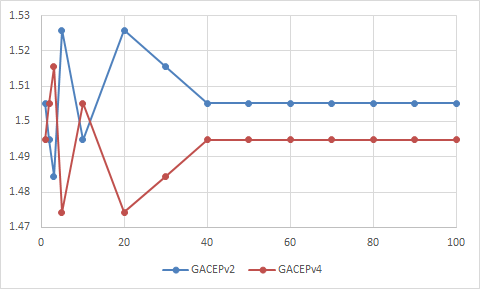
\includegraphics[width=\textwidth]{imagenes/Experimental/GACEPv2vsGACEPv4.png}
         \caption{Ranking durante todas las \textit{milestones}}
         \label{fig:GACEPv2vsGACEPv4_lineas}
     \end{subfigure}
     \hfill
     \begin{subfigure}[b]{0.45\textwidth}
         \centering
         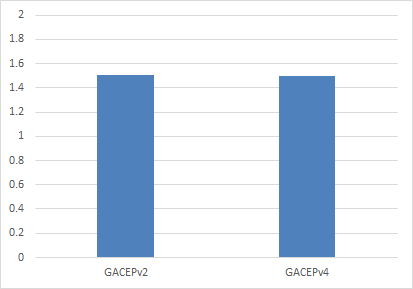
\includegraphics[width=\textwidth]{imagenes/Experimental/barras/GACEPv2vsGACEPv4.png}
         \caption{Ranking final}
         \label{fig:GACEPv2vsGACEPv4_barras}
     \end{subfigure}
        \caption{Comparación de los resultados de GACEPv2 y GACEPv4}
        \label{fig:GACEPv2vsGACEPv4}
\end{figure}

\subsection{Versión del NAM}

La motivación de esta modificación es que el cruce de dos padres lo suficientemente diferentes dará probablemente lugar a un par de soluciones que sean diferentes de ambos padres. 
En esta versión del NAM elegimos el primer padre mediante un Torneo Binario, para garantizar cierta bondad, y el segundo padre mediante el método original: escoger un subconjunto de la población y elegir como padre aquella solución más diferente al primer padre. 
Para esta modificación no hay ningún tipo de umbral de diferencias que se deba pasar para elegir al segundo padre, solo que sea lo más distinto posible. 

Esta versión tomará el nombre de \textbf{GACEPv5}. 

Esta versión ya si supone una gran modificación del propio algoritmo, por lo que es necesario obtener sus resultados \color{red} METER TABLA EN APÉNDICE \color{black} y compararlos con GACEPv2 para determinar si supone una mejora. 
Esta comparación es visible en la gráfica \ref{fig:GACEPv2vsGACEPv5}.

\begin{figure}[h]
     \centering
     \begin{subfigure}[b]{0.45\textwidth}
         \centering
         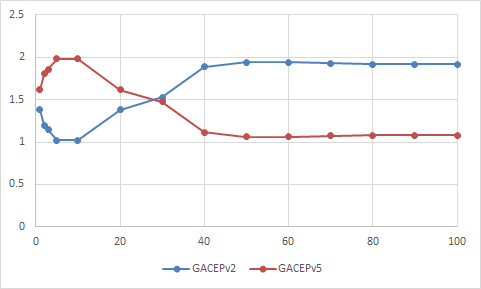
\includegraphics[width=\textwidth]{imagenes/Experimental/GACEPv2vsGACEPv5.png}
         \caption{Ranking durante todas las \textit{milestones}}
         \label{fig:GACEPv2vsGACEPv5_lineas}
     \end{subfigure}
     \hfill
     \begin{subfigure}[b]{0.45\textwidth}
         \centering
         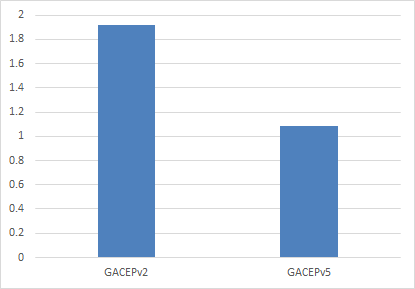
\includegraphics[width=\textwidth]{imagenes/Experimental/barras/GACEPv2vsGACEPv5.png}
         \caption{Ranking final}
         \label{fig:GACEPv2vsGACEPv5_barras}
     \end{subfigure}
        \caption{Comparación de los resultados de GACEPv2 y GACEPv5}
        \label{fig:GACEPv2vsGACEPv5}
\end{figure}

En la gráfica \ref{fig:GACEPv2vsGACEPv5_lineas} se puede ver que, aunque GACEPv2 obtiene resultados mejores en prácticamente todos los casos probados, a partir del 40\% de las ejecuciones se tiene que GACEPv5 mejora a GACEPv2 en casi todas las instancias del problema probadas. 
Por lo tanto, podemos declarar que esta modificación supone una mejora. 

\subsection{Versión del \textit{Crowding} Determinístico}

La motivación de esta modificación es que el criterio para determinar si una nueva solución se introduce o no en la población no sea únicamente el valor de dicha solución, si no también tener en cuenta si aporta diversidad. 
Es decir, dada una solución nueva se deberá buscar en primer lugar aquella solución en la población con la que más parecido tenga y la sustituirá si, y solo si, la supera en valor. 

Esta versión tomará el nombre de \textbf{GACEPv6}. 

De la misma forma que con la introducción del NAM, esta versión supone una gran modificación del propio algoritmo, por lo que es necesario obtener sus resultados \color{red} METER TABLA EN APÉNDICE \color{black} y compararlos con GACEPv2 para determinar si se ha producido una mejora. 
Esta comparación es visible en la gráfica \ref{fig:GACEPv2vsGACEPv6}.

\begin{figure}[h]
     \centering
     \begin{subfigure}[b]{0.45\textwidth}
         \centering
         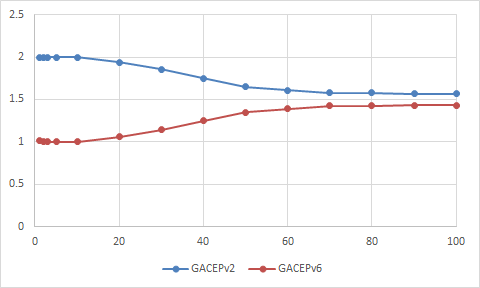
\includegraphics[width=\textwidth]{imagenes/Experimental/GACEPv2vsGACEPv6.png}
         \caption{Ranking durante todas las \textit{milestones}}
         \label{fig:GACEPv2vsGACEPv6_lineas}
     \end{subfigure}
     \hfill
     \begin{subfigure}[b]{0.45\textwidth}
         \centering
         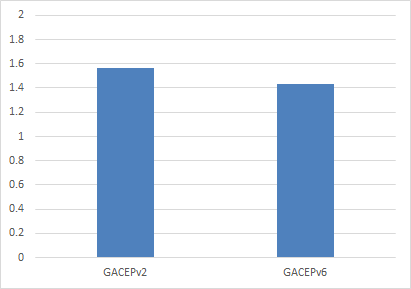
\includegraphics[width=\textwidth]{imagenes/Experimental/barras/GACEPv2vsGACEPv6.png}
         \caption{Ranking final}
         \label{fig:GACEPv2vsGACEPv6_barras}
     \end{subfigure}
        \caption{Comparación de los resultados de GACEPv2 y GACEPv6}
        \label{fig:GACEPv2vsGACEPv6}
\end{figure}

En la gráfica \ref{fig:GACEPv2vsGACEPv6_lineas} se puede comprobar que la nueva versión es mejor en todas las \textit{milestones} que GACEPv2. 
Sin embargo, es importante notar que solo se obtienen mejoras significantes durante la primera mitad de las iteraciones. 


\subsubsection{Reemplazo intensivo}

Esta versión \ref{alg:ORCv} intensifica la idea anterior, ya que no solo podrá sustituir a la solución más cercana, sino que en caso de que lo haga, se llevará un proceso de búsqueda en la población de soluciones tengan menos de cierta cantidad de diferencias con la nueva solución y nos quedaremos únicamente con aquella que sea mejor que el resto. 
En tanto que el tamaño de la población debe ser constante, el resto de soluciones serán sustituidas por soluciones generadas aleatoriamente. 
Nótese que dicho umbral de diferencia va a ser el mismo que se ha aplicado para generar una población inicial diversa y que las soluciones generadas aleatoriamente también deberán cumplir que sean lo suficientemente diversas con respecto a la población en las que son introducidas. 

Esta versión tomará el nombre de \textbf{GACEPv7}. 

En tanto que es una modificación directa sobre GACEPv6, debemos comprobar primero si se consiguen mejorar los resultados sobre esta versión. 
Los resultados obtenidos de la ejecución de GACEPv7 se pueden encontrar en la tabla \color{red} METER TABLA EN APÉNDICE \color{black} y su comparación con los resultados de GACEPv6 se puede visualizar en la gráfica \ref{fig:GACEPv6vsGACEPv7} (se ha cambiado el formato de las gráficas para una mejor visualización).

\begin{figure}[h]
		\centering
		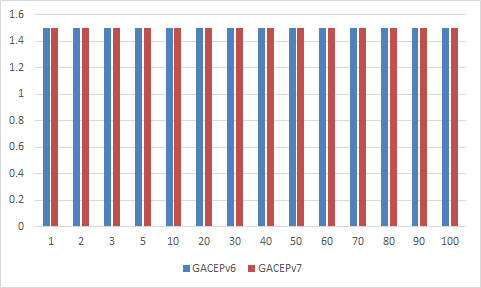
\includegraphics[scale=1]{imagenes/Experimental/barras/GACEPv6vsGACEPv7.png}
        \caption{Comparación de los resultados de GACEPv6 y GACEPv7}
        \label{fig:GACEPv6vsGACEPv7}
\end{figure}

Como se puede observar en la gráfica \ref{fig:GACEPv6vsGACEPv7}, ambas versiones dan exactamente los mismos resultados en todo momento. 
De hecho, tras obtener estos resultados se realizó un estudio de cuál era la causa y resultó que por cada hijo que se iba a introducir en la población había una o ninguna solución existente en la población dentro de este umbral, por lo que el número de soluciones a comprobar siempre era constante: una. 
Ya que incluso si no hay ninguna solución en dicho umbral, por la versión anterior se debe elegir aquella con mayor parecido para compararlas. 
Por lo tanto, esta última modificación nunca se aplicaba. 
Si bien no se ha producido ninguna mejora y descartaremos esta versión, esto nos ha ayudado a descubrir que de cierta forma se está manteniendo cierta diversidad en la población, que era el objetivo de esta sección. 

\subsection{Combinaciones}

Para este apartado, para simplificar la notación que podría llegar a tener el nombre de los algoritmos de las distintas combinaciones, estableceremos que se denominarán ``\textbf{GACEPv\texttt{xy}}'', donde \texttt{x}, \texttt{y} son dos versiones distintas de las introducidas en esta sección. 

En esta sección se han obtenido resultados bastante prometedores que en todos casos mejora a su algoritmo base, GACEPv2. 
Por lo que ahora procederemos a analizar posibles combinaciones de dichas modificaciones por si pudiesen mejorar los resultados actuales obtenidos usando GACEPv2. 

\subsubsection{GACEPv35}

En primer lugar, volvemos a considerar la posibilidad de usar un operador de cruce intensivo, dado establecimos la posibilidad de que su aplicación no aportaba buenos resultados debido a la falta de diversidad. 
En tanto que con estas nuevas modificaciones conseguimos aumentar la diversidad, es una buena idea probar de nuevo su comportamiento junto con la adición de la versión del operador NAM. 
Los resultados de las ejecuciones de esta versión para los distintos porcentajes se encuentran en \color{red} METER TABLA EN APÉNDICE \color{black}.

En la gráfica \ref{fig:GACEPv35} se puede observar el comportamiento de esta nueva versión para los distintos porcentajes.
 
\begin{figure}[h]
     \centering
     \begin{subfigure}[b]{0.45\textwidth}
         \centering
         \includegraphics[width=\textwidth]{imagenes/Experimental/GACEPv35.png}
         \caption{Ranking durante todas las \textit{milestones}}
         \label{fig:GACEPv35_lineas}
     \end{subfigure}
     \hfill
     \begin{subfigure}[b]{0.45\textwidth}
         \centering
         \includegraphics[width=\textwidth]{imagenes/Experimental/barras/GACEPv35.png}
         \caption{Ranking final}
         \label{fig:GACEPv35_barras}
     \end{subfigure}
        \caption{Comparación de los resultados de los GACEPv35c\texttt{x}}
        \label{fig:GACEPv35}
\end{figure}

Se puede apreciar en \ref{fig:GACEPv35_lineas} que el cruce intensivo sigue presentando las mismas características que \ref{fig:GACEPv3cGRASP_lineas} y \ref{fig:GACEPv3cwo_lineas}, donde los resultados son peores cuanto mayor sea la intensidad con la que se aplique este operador de cruce. 
Aunque también es verdad que en este caso los porcentajes 50\%, 60\% y 70\% tienen rendimiento similar durante el primer 30\% de las iteraciones y el \textit{ranking} del 60\% se mantiene cercano al del 50\% durante toda la ejecución. 
Por lo que el mejor porcentaje para esta modificación sería el del 50\%.

\subsubsection{GACEPv36}

A continuación, consideramos la posibilidad de usar de nuevo el operador de cruce intensivo, pero esta vez junto con la versión que implementaba la modificación del operador de reemplazo. 
La motivación de esta versión es la misma que la de GACEPv35, se le quiere dar una nueva oportunidad al operador de cruce intensivo ahora que se ha aumentado la diversidad de la población en todo momento de la ejecución. 
Los resultados de las ejecuciones de esta versión para los distintos porcentajes se encuentran en \color{red} METER TABLA EN APÉNDICE \color{black}.

En la gráfica \ref{fig:GACEPv36} se puede observar el comportamiento de esta nueva versión para los distintos porcentajes. 

\begin{figure}[h]
     \centering
     \begin{subfigure}[b]{0.45\textwidth}
         \centering
         \includegraphics[width=\textwidth]{imagenes/Experimental/GACEPv36.png}
         \caption{Ranking durante todas las \textit{milestones}}
         \label{fig:GACEPv36_lineas}
     \end{subfigure}
     \hfill
     \begin{subfigure}[b]{0.45\textwidth}
         \centering
         \includegraphics[width=\textwidth]{imagenes/Experimental/barras/GACEPv36.png}
         \caption{Ranking final}
         \label{fig:GACEPv36_barras}
     \end{subfigure}
        \caption{Comparación de los resultados de los GACEPv36c\texttt{x}}
        \label{fig:GACEPv36}
\end{figure}

En este caso se puede observar en \ref{fig:GACEPv36_lineas} que GACEPv36 tiene un comportamiento muy similar al GACEPv35 en \ref{fig:GACEPv35_lineas} en tanto que a mayor sea la intensidad del cruce peores serán los resultados y que el cruce para los porcentajes 50\% y 60\% tienen rendimientos algo más similares. 
En definitiva, el mejor porcentaje a utilizar para esta versión sería el del 50\%.

\subsubsection{GACEPv56}

En esta versión se quiere combinar las dos nuevas modificaciones de esta sección: la modificación del operador de selección de padres y la modificación del operador de reemplazo. 
La motivación de esta versión viene dada al observar las gráficas \ref{fig:GACEPv2vsGACEPv5_lineas} y \ref{fig:GACEPv2vsGACEPv6_lineas}. 
Como mencionamos respectivamente en los apartados de estas versiones, GACEPv5 consigue superar en prácticamente todos los casos a GACEPv2, pero solo a partir del 30\% de las iteraciones; mientras que GACEPv6, aunque supera a GACEPv2 para todas las \textit{milestones}, esta mejora es solo notable hasta la primera mitad de las iteraciones. 
Por ello, con esta modificación se pretende combinar ambos comportamientos para que el algoritmo sea consistentemente mejor que GACEPv2. 
Los resultados de las ejecuciones de esta versión se encuentran en \color{red} METER TABLA EN APÉNDICE \color{black}.


\subsubsection{GACEPv356}

Finalmente, consideramos introducir el operador de cruce intensivo en la versión GACEPv56 basándonos en que las suposiciones sobre el comportamiento de GACEPv56. 
La motivación de esta versión es que dicha suposición consiga mejorar el comportamiento que tiene el cruce intensivo convirtiéndolo en una versión más competente. 
Los resultados de las ejecuciones de esta versión para los distintos porcentajes se encuentran en \color{red} METER TABLA EN APÉNDICE \color{black}. 

En la gráfica \ref{fig:GACEPv356} se puede observar el comportamiento de esta nueva versión para los distintos porcentajes. 

\begin{figure}[h]
     \centering
     \begin{subfigure}[b]{0.45\textwidth}
         \centering
         \includegraphics[width=\textwidth]{imagenes/Experimental/GACEPv356.png}
         \caption{Ranking durante todas las \textit{milestones}}
         \label{fig:GACEPv356_lineas}
     \end{subfigure}
     \hfill
     \begin{subfigure}[b]{0.45\textwidth}
         \centering
         \includegraphics[width=\textwidth]{imagenes/Experimental/barras/GACEPv356.png}
         \caption{Ranking final}
         \label{fig:GACEPv356_barras}
     \end{subfigure}
        \caption{Comparación de los resultados de los GACEPv356c\texttt{x}}
        \label{fig:GACEPv356}
\end{figure}

En la gráfica \ref{fig:GACEPv356_lineas} se visualiza que, a grandes rasgos, se sigue manteniendo el comportamiento que lleva presentando a lo largo del trabajo, a mayor intensidad de cruce se tienen peores resultados. 
Además, los \textit{ranking} del 50\% y del 60\% se mantienen parecido durante la mayoría de las iteraciones. 
Como novedad, se puede ver que este ha sido el único caso en el que 80\% ha tenido resultados parecidos al resto durante un breve periodo de iteraciones (en el resto de casos siempre ha sido en todo momento bastante peor).

\subsection{Comparaciones}

En este apartado se compararán todas las versiones a la vez junto con GACEPv2 para tener una visión global de los resultados que se han obtenido para esta sección y poder determinar de forma definitiva si se ha producido alguna mejora significativa y cuál versión es la mejor. 

En la gráfica \ref{fig:GACEP3103vsGACEPv2} vienen representado los \textit{ranking} de cada una de las versiones para las distintas \textit{milestones} junto con una gráfica de barras  para indicar el \textit{ranking} final de dichas versiones. 

\begin{figure}[h]
     \centering
     \begin{subfigure}[b]{0.45\textwidth}
         \centering
         \includegraphics[width=\textwidth]{imagenes/Experimental/GACEP3103vsGACEPv2.png}
         \caption{Ranking durante todas las \textit{milestones}}
         \label{fig:GACEP3103vsGACEPv2_lineas}
     \end{subfigure}
     \hfill
     \begin{subfigure}[b]{0.45\textwidth}
         \centering
         \includegraphics[width=\textwidth]{imagenes/Experimental/barras/GACEP3103vsGACEPv2.png}
         \caption{Ranking final}
         \label{fig:GACEP3103vsGACEPv2_barras}
     \end{subfigure}
        \caption{Comparación de los resultados de las versiones de esta sección con GACEPv2}
        \label{fig:GACEP3103vsGACEPv2}
\end{figure}

Como se puede comprobar en \ref{fig:GACEP3103vsGACEPv2_lineas} todas las versiones excepto GACEPv36 ofrecen mejores resultados las instancias del problema con las que hemos trabajado. 
Recuérdese que GACEPv4 aportaba unos resultados muy parecidos a GACEPv2, por lo que en \ref{fig:GACEP3103vsGACEPv2_lineas} se visualiza como la misma línea. 
Es interesante mencionar que GACEPv5 y GACEPv35 presentan un comportamiento muy similar, en las primeras iteraciones aportan los peores resultados y a medida que avanza la ejecución logra mejorar la mitad de las versiones, aunque GACEPv35 resulta ser vagamente peor. 
En contraposición, nos encontramos con GACEPv6 y GACEPv36, que presentan un comportamiento muy similar, en las primeras iteraciones aportan buenos resultados y a medida que avanza la ejecución obtiene peores resultados comparándolos con el resto de versiones, aunque en este caso la versión con cruce intensivo resulta bastante peor que la versión sin cruce intensivo. 
Por otra parte, el \textit{ranking} de GACEPv356 se mantiene relativamente constante durante todas las iteraciones aportando uno de los mejores resultados, aunque en la segunda mitad de la ejecución su \textit{ranking} converge con el de GACEPv5 y GACEPv35; de hecho, al final consigue el mismo \textit{ranking} que GACEPv35, siendo peor que GACEPv5 por una diferencia de centésimas. 
Con esto llegamos a la conclusión definitiva que la introducción de cruce intensivo en el algoritmo no logra mejorarlo en ningún momento, como máximo es capaz de lograr resultados similares. 

Finalmente, y más importante, hemos descubierto cuál es la mejor versión y la que consideraremos la versión final de este proceso de diseño de metaheurísticas. 
Se tiene que GACEPv56 es consistemente la mejor versión entre todas las presentadas en esta sección. 
Con eso se confirma nuestra hipótesis, presentada anteriormente, de que el uso de la versión de NAM y el cambio del operador de reemplazo iba a suponer la mezcla de los mejores comportamientos de cada versión individual: ser mejor que GACEPv2 en la mayoría de los casos durante la primera mitad de la ejecución (GACEPv6) y ser mejor que GACEPv2 en la mayoría de los casos durante la segunda mitad de la ejecución (GACEPv5).

Tras esto, mostraremos una tabla \ref{DiferenciasGACEPv56} y su gráfica \ref{fig:DiferenciasGACEPv56} asociada sobre las diferencias entre las mejores soluciones de cada \textit{milestone} para poder comprobar su evolución. 

\begin{table}[h]
\begin{tabular}{|cclcclccl|}
\hline
\rowcolor[HTML]{FFFFC7} 
\multicolumn{9}{|c|}{\cellcolor[HTML]{FFFFC7}GACEPv56}                                                                                                                                                                                                                                                                                                                                                                                                                                                                                                  \\ \hline
\rowcolor[HTML]{F7EAC7} 
\multicolumn{1}{|c|}{\cellcolor[HTML]{F7EAC7}n}                               & \multicolumn{1}{c|}{\cellcolor[HTML]{F7EAC7}milestone} & \multicolumn{1}{l|}{\cellcolor[HTML]{F7EAC7}Diferencia} & \multicolumn{1}{c|}{\cellcolor[HTML]{F7EAC7}n}                               & \multicolumn{1}{c|}{\cellcolor[HTML]{F7EAC7}milestone} & \multicolumn{1}{l|}{\cellcolor[HTML]{F7EAC7}Diferencia} & \multicolumn{1}{c|}{\cellcolor[HTML]{F7EAC7}n}                               & \multicolumn{1}{c|}{\cellcolor[HTML]{F7EAC7}milestone} & Diferencia \\ \hline
\rowcolor[HTML]{DAE8FC} 
\multicolumn{1}{|c|}{\cellcolor[HTML]{FFFFC7}}                                & \multicolumn{1}{c|}{\cellcolor[HTML]{DAE8FC}1}         & \multicolumn{1}{l|}{\cellcolor[HTML]{DAE8FC}21.8623}    & \multicolumn{1}{c|}{\cellcolor[HTML]{FFFFC7}}                                & \multicolumn{1}{c|}{\cellcolor[HTML]{DAE8FC}1}         & \multicolumn{1}{l|}{\cellcolor[HTML]{DAE8FC}25.5970838} & \multicolumn{1}{c|}{\cellcolor[HTML]{FFFFC7}}                                & \multicolumn{1}{c|}{\cellcolor[HTML]{DAE8FC}1}         & 25.4820586 \\ \cline{2-3} \cline{5-6} \cline{8-9} 
\rowcolor[HTML]{DDFDFF} 
\multicolumn{1}{|c|}{\cellcolor[HTML]{FFFFC7}}                                & \multicolumn{1}{c|}{\cellcolor[HTML]{DDFDFF}2}         & \multicolumn{1}{l|}{\cellcolor[HTML]{DDFDFF}18.0516}    & \multicolumn{1}{c|}{\cellcolor[HTML]{FFFFC7}}                                & \multicolumn{1}{c|}{\cellcolor[HTML]{DDFDFF}2}         & \multicolumn{1}{l|}{\cellcolor[HTML]{DDFDFF}21.1200773} & \multicolumn{1}{c|}{\cellcolor[HTML]{FFFFC7}}                                & \multicolumn{1}{c|}{\cellcolor[HTML]{DDFDFF}2}         & 20.90983   \\ \cline{2-3} \cline{5-6} \cline{8-9} 
\rowcolor[HTML]{DAE8FC} 
\multicolumn{1}{|c|}{\cellcolor[HTML]{FFFFC7}}                                & \multicolumn{1}{c|}{\cellcolor[HTML]{DAE8FC}3}         & \multicolumn{1}{l|}{\cellcolor[HTML]{DAE8FC}16.1184}    & \multicolumn{1}{c|}{\cellcolor[HTML]{FFFFC7}}                                & \multicolumn{1}{c|}{\cellcolor[HTML]{DAE8FC}3}         & \multicolumn{1}{l|}{\cellcolor[HTML]{DAE8FC}18.7431685} & \multicolumn{1}{c|}{\cellcolor[HTML]{FFFFC7}}                                & \multicolumn{1}{c|}{\cellcolor[HTML]{DAE8FC}3}         & 18.3898234 \\ \cline{2-3} \cline{5-6} \cline{8-9} 
\rowcolor[HTML]{DDFDFF} 
\multicolumn{1}{|c|}{\cellcolor[HTML]{FFFFC7}}                                & \multicolumn{1}{c|}{\cellcolor[HTML]{DDFDFF}5}         & \multicolumn{1}{l|}{\cellcolor[HTML]{DDFDFF}13.1784}    & \multicolumn{1}{c|}{\cellcolor[HTML]{FFFFC7}}                                & \multicolumn{1}{c|}{\cellcolor[HTML]{DDFDFF}5}         & \multicolumn{1}{l|}{\cellcolor[HTML]{DDFDFF}14.8269699} & \multicolumn{1}{c|}{\cellcolor[HTML]{FFFFC7}}                                & \multicolumn{1}{c|}{\cellcolor[HTML]{DDFDFF}5}         & 14.3143042 \\ \cline{2-3} \cline{5-6} \cline{8-9} 
\rowcolor[HTML]{DAE8FC} 
\multicolumn{1}{|c|}{\cellcolor[HTML]{FFFFC7}}                                & \multicolumn{1}{c|}{\cellcolor[HTML]{DAE8FC}10}        & \multicolumn{1}{l|}{\cellcolor[HTML]{DAE8FC}9.95847}    & \multicolumn{1}{c|}{\cellcolor[HTML]{FFFFC7}}                                & \multicolumn{1}{c|}{\cellcolor[HTML]{DAE8FC}10}        & \multicolumn{1}{l|}{\cellcolor[HTML]{DAE8FC}9.47807895} & \multicolumn{1}{c|}{\cellcolor[HTML]{FFFFC7}}                                & \multicolumn{1}{c|}{\cellcolor[HTML]{DAE8FC}10}        & 8.7815101  \\ \cline{2-3} \cline{5-6} \cline{8-9} 
\rowcolor[HTML]{DDFDFF} 
\multicolumn{1}{|c|}{\cellcolor[HTML]{FFFFC7}}                                & \multicolumn{1}{c|}{\cellcolor[HTML]{DDFDFF}20}        & \multicolumn{1}{l|}{\cellcolor[HTML]{DDFDFF}4.83628}    & \multicolumn{1}{c|}{\cellcolor[HTML]{FFFFC7}}                                & \multicolumn{1}{c|}{\cellcolor[HTML]{DDFDFF}20}        & \multicolumn{1}{l|}{\cellcolor[HTML]{DDFDFF}5.73939044} & \multicolumn{1}{c|}{\cellcolor[HTML]{FFFFC7}}                                & \multicolumn{1}{c|}{\cellcolor[HTML]{DDFDFF}20}        & 5.27891921 \\ \cline{2-3} \cline{5-6} \cline{8-9} 
\rowcolor[HTML]{DAE8FC} 
\multicolumn{1}{|c|}{\cellcolor[HTML]{FFFFC7}}                                & \multicolumn{1}{c|}{\cellcolor[HTML]{DAE8FC}30}        & \multicolumn{1}{l|}{\cellcolor[HTML]{DAE8FC}4.23393}    & \multicolumn{1}{c|}{\cellcolor[HTML]{FFFFC7}}                                & \multicolumn{1}{c|}{\cellcolor[HTML]{DAE8FC}30}        & \multicolumn{1}{l|}{\cellcolor[HTML]{DAE8FC}4.36629592} & \multicolumn{1}{c|}{\cellcolor[HTML]{FFFFC7}}                                & \multicolumn{1}{c|}{\cellcolor[HTML]{DAE8FC}30}        & 3.87182862 \\ \cline{2-3} \cline{5-6} \cline{8-9} 
\rowcolor[HTML]{DDFDFF} 
\multicolumn{1}{|c|}{\cellcolor[HTML]{FFFFC7}}                                & \multicolumn{1}{c|}{\cellcolor[HTML]{DDFDFF}40}        & \multicolumn{1}{l|}{\cellcolor[HTML]{DDFDFF}0.13499}    & \multicolumn{1}{c|}{\cellcolor[HTML]{FFFFC7}}                                & \multicolumn{1}{c|}{\cellcolor[HTML]{DDFDFF}40}        & \multicolumn{1}{l|}{\cellcolor[HTML]{DDFDFF}0.65991695} & \multicolumn{1}{c|}{\cellcolor[HTML]{FFFFC7}}                                & \multicolumn{1}{c|}{\cellcolor[HTML]{DDFDFF}40}        & 1.00562574 \\ \cline{2-3} \cline{5-6} \cline{8-9} 
\rowcolor[HTML]{DAE8FC} 
\multicolumn{1}{|c|}{\cellcolor[HTML]{FFFFC7}}                                & \multicolumn{1}{c|}{\cellcolor[HTML]{DAE8FC}50}        & \multicolumn{1}{l|}{\cellcolor[HTML]{DAE8FC}0.08385}    & \multicolumn{1}{c|}{\cellcolor[HTML]{FFFFC7}}                                & \multicolumn{1}{c|}{\cellcolor[HTML]{DAE8FC}50}        & \multicolumn{1}{l|}{\cellcolor[HTML]{DAE8FC}0.18139206} & \multicolumn{1}{c|}{\cellcolor[HTML]{FFFFC7}}                                & \multicolumn{1}{c|}{\cellcolor[HTML]{DAE8FC}50}        & 0.49856815 \\ \cline{2-3} \cline{5-6} \cline{8-9} 
\rowcolor[HTML]{DDFDFF} 
\multicolumn{1}{|c|}{\cellcolor[HTML]{FFFFC7}}                                & \multicolumn{1}{c|}{\cellcolor[HTML]{DDFDFF}60}        & \multicolumn{1}{l|}{\cellcolor[HTML]{DDFDFF}0.01782}    & \multicolumn{1}{c|}{\cellcolor[HTML]{FFFFC7}}                                & \multicolumn{1}{c|}{\cellcolor[HTML]{DDFDFF}60}        & \multicolumn{1}{l|}{\cellcolor[HTML]{DDFDFF}0.02886742} & \multicolumn{1}{c|}{\cellcolor[HTML]{FFFFC7}}                                & \multicolumn{1}{c|}{\cellcolor[HTML]{DDFDFF}60}        & 0.11276472 \\ \cline{2-3} \cline{5-6} \cline{8-9} 
\rowcolor[HTML]{DAE8FC} 
\multicolumn{1}{|c|}{\cellcolor[HTML]{FFFFC7}}                                & \multicolumn{1}{c|}{\cellcolor[HTML]{DAE8FC}70}        & \multicolumn{1}{l|}{\cellcolor[HTML]{DAE8FC}0.01597}    & \multicolumn{1}{c|}{\cellcolor[HTML]{FFFFC7}}                                & \multicolumn{1}{c|}{\cellcolor[HTML]{DAE8FC}70}        & \multicolumn{1}{l|}{\cellcolor[HTML]{DAE8FC}0.01139917} & \multicolumn{1}{c|}{\cellcolor[HTML]{FFFFC7}}                                & \multicolumn{1}{c|}{\cellcolor[HTML]{DAE8FC}70}        & 0.01587516 \\ \cline{2-3} \cline{5-6} \cline{8-9} 
\rowcolor[HTML]{DDFDFF} 
\multicolumn{1}{|c|}{\cellcolor[HTML]{FFFFC7}}                                & \multicolumn{1}{c|}{\cellcolor[HTML]{DDFDFF}80}        & \multicolumn{1}{l|}{\cellcolor[HTML]{DDFDFF}0}          & \multicolumn{1}{c|}{\cellcolor[HTML]{FFFFC7}}                                & \multicolumn{1}{c|}{\cellcolor[HTML]{DDFDFF}80}        & \multicolumn{1}{l|}{\cellcolor[HTML]{DDFDFF}0}          & \multicolumn{1}{c|}{\cellcolor[HTML]{FFFFC7}}                                & \multicolumn{1}{c|}{\cellcolor[HTML]{DDFDFF}80}        & 0.00745689 \\ \cline{2-3} \cline{5-6} \cline{8-9} 
\rowcolor[HTML]{DAE8FC} 
\multicolumn{1}{|c|}{\multirow{-13}{*}{\cellcolor[HTML]{FFFFC7}\textbf{100}}} & \multicolumn{1}{c|}{\cellcolor[HTML]{DAE8FC}90}        & \multicolumn{1}{l|}{\cellcolor[HTML]{DAE8FC}0}          & \multicolumn{1}{c|}{\multirow{-13}{*}{\cellcolor[HTML]{FFFFC7}\textbf{200}}} & \multicolumn{1}{c|}{\cellcolor[HTML]{DAE8FC}90}        & \multicolumn{1}{l|}{\cellcolor[HTML]{DAE8FC}0}          & \multicolumn{1}{c|}{\multirow{-13}{*}{\cellcolor[HTML]{FFFFC7}\textbf{300}}} & \multicolumn{1}{c|}{\cellcolor[HTML]{DAE8FC}90}        & 0          \\ \hline
\end{tabular}
\caption{\label{DiferenciasGACEPv56}Diferencias de los resultados de las distintas milestones con respecto a la final para el algoritmo GACEPv56}
\end{table}

\begin{figure}[h]
		\centering
		\includegraphics[scale=1]{imagenes/Experimental/DiferenciasGACEPv56.png}
        \caption{Gráfica asociada a la tabla \ref{DiferenciasGACEPv56}}
        \label{fig:DiferenciasGACEPv56}
\end{figure}


Por tanto, a la versión de GACEPv56 se le considerará la versión final, a la que nombraremos \textbf{GACEPvf}.

\section{Comparación final}

En esta sección se compararán todas las versiones más destacables (AGEU, GACEPv1, GACEPv2 y GACEPv3c50) con la versión final, GACEPvf. 

En primer lugar, mostraremos una gráfica \ref{fig:Final} con los \textit{ranking} de cada una de las versiones para las distintas \textit{milestones} junto con una gráfica de barras para indicar el \textit{ranking} final de dichas versiones. 

\begin{figure}[h]
     \centering
     \begin{subfigure}[b]{0.45\textwidth}
         \centering
         \includegraphics[width=\textwidth]{imagenes/Experimental/Final.png}
         \caption{Ranking durante todas las \textit{milestones}}
         \label{fig:Final_lineas}
     \end{subfigure}
     \hfill
     \begin{subfigure}[b]{0.45\textwidth}
         \centering
         \includegraphics[width=\textwidth]{imagenes/Experimental/barras/Final.png}
         \caption{Ranking final}
         \label{fig:Final_barras}
     \end{subfigure}
        \caption{Comparación de los resultados de las versiones de esta sección con GACEPv2}
        \label{fig:Final}
\end{figure}

En la gráfica \ref{fig:Final_lineas} se puede comprobar como nuestra versión final del algoritmo es mejor que el resto para prácticamente todas las instancias del problema con las que hemos trabajado en todo momento de la ejecución. 
Por otra parte, podemos observar en \ref{fig:Final_barras} cómo la clasificación de las distintas versiones presentadas ha ido mejorando a las anteriores.

Finalizaremos esta comparación haciendo uso de un test estadístico no paramétrico para comparaciones múltiples mostrado en la Tabla \ref{TestFinal}.

\begin{table}[h]
\begin{tabular}{|c|c|c|c|c|}
\hline
\multicolumn{1}{|l|}{Algorithms vs  GACEPvf} & \textbf{Original} & \textbf{Holm}                   & \textbf{Hommel}                 & \textbf{Hochberg}               \\ \hline
\textbf{AGEU}                                & 1.24E-17          & {\color[HTML]{0000FF} 4.95E-17} & {\color[HTML]{0000FF} 3.25E-17} & {\color[HTML]{0000FF} 3.66E-17} \\ \hline
\textbf{GACEPv1}                             & 3.66E-17          & {\color[HTML]{0000FF} 4.95E-17} & {\color[HTML]{0000FF} 3.66E-17} & {\color[HTML]{0000FF} 3.66E-17} \\ \hline
\textbf{GACEPv2}                             & 2.16E-17          & {\color[HTML]{0000FF} 4.95E-17} & {\color[HTML]{0000FF} 3.66E-17} & {\color[HTML]{0000FF} 3.66E-17} \\ \hline
\textbf{GACEPv3c50}                          & 1.28E-17          & {\color[HTML]{0000FF} 4.95E-17} & {\color[HTML]{0000FF} 3.25E-17} & {\color[HTML]{0000FF} 3.66E-17} \\ \hline
\end{tabular}
\caption{\label{TestFinal}Test de $p$-valores para comparaciones múltiples referente la comparación final (Error Global: 5\%)}
\end{table}

\color{red}
No sé muy bien como interpretarlo
\color{black}

\section{Resumen de las versiones}

A modo de resumen de este capítulo, reuniremos todas las versiones mencionadas en una tabla \ref{ResumenVersiones}.

\begin{table}[h]
\begin{tabular}{|l|l|l|}
\hline
\rowcolor[HTML]{FFFFC7} 
Algoritmo   & Base       & Descripción                                                                                                                                    \\ \hline
\rowcolor[HTML]{DAE8FC} 
AGEU        &            & Algoritmo de referencia AGEU ejecutado con 450 iteraciones                                                                                     \\ \hline
\rowcolor[HTML]{DDFDFF} 
GACEPv1     & AGEU       & \begin{tabular}[c]{@{}l@{}}Se introduce el histórico para el Operador de Reparación\\ y Mutación\end{tabular}                                  \\ \hline
\rowcolor[HTML]{DAE8FC} 
GACEPv2     & GACEPv1    & Se introduce GRASP al Operador de Reparación                                                                                                   \\ \hline
\rowcolor[HTML]{DDFDFF} 
GACEPv3cx   & GACEPv2    & \begin{tabular}[c]{@{}l@{}}Se modifica el operador de cruce a un Operador de Cruce \\ Intensivo, en vez de usar un Cruce Uniforme\end{tabular} \\ \hline
\rowcolor[HTML]{DAE8FC} 
GACEPv3cxwo & GACEPv1    & \begin{tabular}[c]{@{}l@{}}Se modifica el operador de cruce a un Operador de Cruce \\ Intensivo, en vez de usar un Cruce Uniforme\end{tabular}                                                                                                                                                \\ \hline
\rowcolor[HTML]{DDFDFF} 
GACEPv4     & GACEPv2    & Se introduce una Población Inicial Diversa                                                                                                     \\ \hline
\rowcolor[HTML]{DAE8FC} 
GACEPv5     & GACEPv4    & Se introduce una versión del Operador NAM                                                                                                      \\ \hline
\rowcolor[HTML]{DDFDFF} 
GACEPv6     & GACEPv4    & Se introduce un nuevo Operador de Reemplazo por Cercanía                                                                                       \\ \hline
\rowcolor[HTML]{DAE8FC} 
GACEPv7     & GACEPv6    & \begin{tabular}[c]{@{}l@{}}Se introduce una intensificación de dicho Operador de\\ Reemplazo\end{tabular}                                      \\ \hline
\rowcolor[HTML]{DDFDFF} 
GACEPv35cx  & GACEPv5    & Se vuelve a introducir el Operador de Cruce Intensivo                                                                                          \\ \hline
\rowcolor[HTML]{DAE8FC} 
GACEPv36cx  & GACEPv6    & Se vuelve a introducir el Operador de Cruce Intensivo                                                                                          \\ \hline
\rowcolor[HTML]{DDFDFF} 
GACEPv56    & GACEPv4    & Se introducen las modificaciones de GACEPv5 y GACEPv6                                                                                          \\ \hline
\rowcolor[HTML]{DAE8FC} 
GACEPv356cx & GACEPv56   & Se vuelve a introducir el Operador de Cruce Intensivo                                                                                          \\ \hline
\rowcolor[HTML]{DDFDFF} 
CHC         &            & Algoritmo de referencia CHC ejecutado con 450 iteraciones                                                                                      \\ \hline
\rowcolor[HTML]{DAE8FC} 
GACEPCHCv1  & CHC        & \begin{tabular}[c]{@{}l@{}}Se introduce el histórico para el Operador de Reparación\\ y Mutación\end{tabular}                                  \\ \hline
\rowcolor[HTML]{DDFDFF} 
GACEPCHCv2  & GACEPCHCv1 & Se introduce GRASP al Operador de Reparación                                                                                                   \\ \hline
\rowcolor[HTML]{DAE8FC} 
GACEPvf     &            & Versión final del algoritmo, será GACEPv56                                                                                                     \\ \hline
\end{tabular}
\caption{\label{ResumenVersiones}Resumen de las distintas versiones de los algoritmos utilizadas}
\end{table}

%
\chapter{Conclusiones}
%%\chapter{Conclusiones y Trabajos Futuros}
%
%
%%\nocite{*}
\printbibliography
\addcontentsline{toc}{chapter}{Bibliografía}
%
\appendix
\chapter{Tablas de Resultados}

%AGEU450
\begin{table}[]
\begin{tabular}{|ccrccrccc}
\hline
\rowcolor[HTML]{FFFFC7} 
\multicolumn{9}{|c|}{\cellcolor[HTML]{FFFFC7}AGEU   450}                                                                                                                                                                                                                                                                                                                                                                                                                                                                                                                                                                               \\ \hline
\rowcolor[HTML]{F7EAC7} 
\multicolumn{1}{|c|}{\cellcolor[HTML]{F7EAC7}n}                               & \multicolumn{1}{c|}{\cellcolor[HTML]{F7EAC7}densidad}              & \multicolumn{1}{c|}{\cellcolor[HTML]{F7EAC7}Resultado} & \multicolumn{1}{c|}{\cellcolor[HTML]{F7EAC7}n}                               & \multicolumn{1}{c|}{\cellcolor[HTML]{F7EAC7}densidad}               & \multicolumn{1}{c|}{\cellcolor[HTML]{F7EAC7}Resultado} & \multicolumn{1}{c|}{\cellcolor[HTML]{F7EAC7}n}                               & \multicolumn{1}{c|}{\cellcolor[HTML]{F7EAC7}densidad}              & \multicolumn{1}{c|}{\cellcolor[HTML]{F7EAC7}Resultado} \\ \hline
\rowcolor[HTML]{DAE8FC} 
\multicolumn{1}{|c|}{\cellcolor[HTML]{FFFFC7}}                                & \multicolumn{1}{c|}{\cellcolor[HTML]{DAE8FC}}                      & \multicolumn{1}{r|}{\cellcolor[HTML]{DAE8FC}192975}    & \multicolumn{1}{c|}{\cellcolor[HTML]{FFFFC7}}                                & \multicolumn{1}{c|}{\cellcolor[HTML]{DAE8FC}}                       & \multicolumn{1}{r|}{\cellcolor[HTML]{DAE8FC}375031}    & \multicolumn{1}{c|}{\cellcolor[HTML]{FFFFC7}}                                & \multicolumn{1}{c|}{\cellcolor[HTML]{DAE8FC}}                      & \multicolumn{1}{r|}{\cellcolor[HTML]{DAE8FC}376494}    \\ \cline{3-3} \cline{6-6} \cline{9-9} 
\multicolumn{1}{|c|}{\cellcolor[HTML]{FFFFC7}}                                & \multicolumn{1}{c|}{\cellcolor[HTML]{DAE8FC}}                      & \multicolumn{1}{r|}{\cellcolor[HTML]{DDFDFF}81641.3}   & \multicolumn{1}{c|}{\cellcolor[HTML]{FFFFC7}}                                & \multicolumn{1}{c|}{\cellcolor[HTML]{DAE8FC}}                       & \multicolumn{1}{r|}{\cellcolor[HTML]{DDFDFF}936531}    & \multicolumn{1}{c|}{\cellcolor[HTML]{FFFFC7}}                                & \multicolumn{1}{c|}{\cellcolor[HTML]{DAE8FC}}                      & \multicolumn{1}{r|}{\cellcolor[HTML]{DDFDFF}28788.7}   \\ \cline{3-3} \cline{6-6} \cline{9-9} 
\rowcolor[HTML]{DAE8FC} 
\multicolumn{1}{|c|}{\cellcolor[HTML]{FFFFC7}}                                & \multicolumn{1}{c|}{\cellcolor[HTML]{DAE8FC}}                      & \multicolumn{1}{r|}{\cellcolor[HTML]{DAE8FC}189162}    & \multicolumn{1}{c|}{\cellcolor[HTML]{FFFFC7}}                                & \multicolumn{1}{c|}{\cellcolor[HTML]{DAE8FC}}                       & \multicolumn{1}{r|}{\cellcolor[HTML]{DAE8FC}302452}    & \multicolumn{1}{c|}{\cellcolor[HTML]{FFFFC7}}                                & \multicolumn{1}{c|}{\cellcolor[HTML]{DAE8FC}}                      & \multicolumn{1}{r|}{\cellcolor[HTML]{DAE8FC}275573}    \\ \cline{3-3} \cline{6-6} \cline{9-9} 
\multicolumn{1}{|c|}{\cellcolor[HTML]{FFFFC7}}                                & \multicolumn{1}{c|}{\cellcolor[HTML]{DAE8FC}}                      & \multicolumn{1}{r|}{\cellcolor[HTML]{DDFDFF}224189}    & \multicolumn{1}{c|}{\cellcolor[HTML]{FFFFC7}}                                & \multicolumn{1}{c|}{\cellcolor[HTML]{DAE8FC}}                       & \multicolumn{1}{r|}{\cellcolor[HTML]{DDFDFF}29203.7}   & \multicolumn{1}{c|}{\cellcolor[HTML]{FFFFC7}}                                & \multicolumn{1}{c|}{\cellcolor[HTML]{DAE8FC}}                      & \multicolumn{1}{r|}{\cellcolor[HTML]{DDFDFF}439862}    \\ \cline{3-3} \cline{6-6} \cline{9-9} 
\rowcolor[HTML]{DAE8FC} 
\multicolumn{1}{|c|}{\cellcolor[HTML]{FFFFC7}}                                & \multicolumn{1}{c|}{\cellcolor[HTML]{DAE8FC}}                      & \multicolumn{1}{r|}{\cellcolor[HTML]{DAE8FC}229585}    & \multicolumn{1}{c|}{\cellcolor[HTML]{FFFFC7}}                                & \multicolumn{1}{c|}{\cellcolor[HTML]{DAE8FC}}                       & \multicolumn{1}{r|}{\cellcolor[HTML]{DAE8FC}100514}    & \multicolumn{1}{c|}{\cellcolor[HTML]{FFFFC7}}                                & \multicolumn{1}{c|}{\cellcolor[HTML]{DAE8FC}}                      & \multicolumn{1}{r|}{\cellcolor[HTML]{DAE8FC}14777.8}   \\ \cline{3-3} \cline{6-6} \cline{9-9} 
\multicolumn{1}{|c|}{\cellcolor[HTML]{FFFFC7}}                                & \multicolumn{1}{c|}{\cellcolor[HTML]{DAE8FC}}                      & \multicolumn{1}{r|}{\cellcolor[HTML]{DDFDFF}73991.5}   & \multicolumn{1}{c|}{\cellcolor[HTML]{FFFFC7}}                                & \multicolumn{1}{c|}{\cellcolor[HTML]{DAE8FC}}                       & \multicolumn{1}{r|}{\cellcolor[HTML]{DDFDFF}779113}    & \multicolumn{1}{c|}{\cellcolor[HTML]{FFFFC7}}                                & \multicolumn{1}{c|}{\cellcolor[HTML]{DAE8FC}}                      & \multicolumn{1}{r|}{\cellcolor[HTML]{DDFDFF}263938}    \\ \cline{3-3} \cline{6-6} \cline{9-9} 
\rowcolor[HTML]{DAE8FC} 
\multicolumn{1}{|c|}{\cellcolor[HTML]{FFFFC7}}                                & \multicolumn{1}{c|}{\cellcolor[HTML]{DAE8FC}}                      & \multicolumn{1}{r|}{\cellcolor[HTML]{DAE8FC}10154.9}   & \multicolumn{1}{c|}{\cellcolor[HTML]{FFFFC7}}                                & \multicolumn{1}{c|}{\cellcolor[HTML]{DAE8FC}}                       & \multicolumn{1}{r|}{\cellcolor[HTML]{DAE8FC}40194.9}   & \multicolumn{1}{c|}{\cellcolor[HTML]{FFFFC7}}                                & \multicolumn{1}{c|}{\cellcolor[HTML]{DAE8FC}}                      & \multicolumn{1}{r|}{\cellcolor[HTML]{DAE8FC}481905}    \\ \cline{3-3} \cline{6-6} \cline{9-9} 
\multicolumn{1}{|c|}{\cellcolor[HTML]{FFFFC7}}                                & \multicolumn{1}{c|}{\cellcolor[HTML]{DAE8FC}}                      & \multicolumn{1}{r|}{\cellcolor[HTML]{DDFDFF}62289.6}   & \multicolumn{1}{c|}{\cellcolor[HTML]{FFFFC7}}                                & \multicolumn{1}{c|}{\cellcolor[HTML]{DAE8FC}}                       & \multicolumn{1}{r|}{\cellcolor[HTML]{DDFDFF}693305}    & \multicolumn{1}{c|}{\cellcolor[HTML]{FFFFC7}}                                & \multicolumn{1}{c|}{\cellcolor[HTML]{DAE8FC}}                      & \multicolumn{1}{r|}{\cellcolor[HTML]{DDFDFF}9176.36}   \\ \cline{3-3} \cline{6-6} \cline{9-9} 
\rowcolor[HTML]{DAE8FC} 
\multicolumn{1}{|c|}{\cellcolor[HTML]{FFFFC7}}                                & \multicolumn{1}{c|}{\cellcolor[HTML]{DAE8FC}}                      & \multicolumn{1}{r|}{\cellcolor[HTML]{DAE8FC}232572}    & \multicolumn{1}{c|}{\cellcolor[HTML]{FFFFC7}}                                & \multicolumn{1}{c|}{\multirow{-9}{*}{\cellcolor[HTML]{DAE8FC}25}}   & \multicolumn{1}{r|}{\cellcolor[HTML]{DAE8FC}779359}    & \multicolumn{1}{c|}{\cellcolor[HTML]{FFFFC7}}                                & \multicolumn{1}{c|}{\multirow{-9}{*}{\cellcolor[HTML]{DAE8FC}25}}  & \multicolumn{1}{r|}{\cellcolor[HTML]{DAE8FC}245377}    \\ \cline{3-3} \cline{5-6} \cline{8-9} 
\multicolumn{1}{|c|}{\cellcolor[HTML]{FFFFC7}}                                & \multicolumn{1}{c|}{\multirow{-10}{*}{\cellcolor[HTML]{DAE8FC}25}} & \multicolumn{1}{r|}{\cellcolor[HTML]{DDFDFF}24729.5}   & \multicolumn{1}{c|}{\cellcolor[HTML]{FFFFC7}}                                & \multicolumn{1}{c|}{\cellcolor[HTML]{DDFDFF}}                       & \multicolumn{1}{r|}{\cellcolor[HTML]{DAE8FC}622413}    & \multicolumn{1}{c|}{\cellcolor[HTML]{FFFFC7}}                                & \multicolumn{1}{c|}{\cellcolor[HTML]{DDFDFF}}                      & \multicolumn{1}{r|}{\cellcolor[HTML]{DAE8FC}990137}    \\ \cline{2-3} \cline{6-6} \cline{9-9} 
\rowcolor[HTML]{DDFDFF} 
\multicolumn{1}{|c|}{\cellcolor[HTML]{FFFFC7}}                                & \multicolumn{1}{c|}{\cellcolor[HTML]{DDFDFF}}                      & \multicolumn{1}{r|}{\cellcolor[HTML]{DAE8FC}18382.8}   & \multicolumn{1}{c|}{\cellcolor[HTML]{FFFFC7}}                                & \multicolumn{1}{c|}{\cellcolor[HTML]{DDFDFF}}                       & \multicolumn{1}{r|}{\cellcolor[HTML]{DDFDFF}47981}     & \multicolumn{1}{c|}{\cellcolor[HTML]{FFFFC7}}                                & \multicolumn{1}{c|}{\cellcolor[HTML]{DDFDFF}}                      & \multicolumn{1}{r|}{\cellcolor[HTML]{DDFDFF}501953}    \\ \cline{3-3} \cline{6-6} \cline{9-9} 
\multicolumn{1}{|c|}{\cellcolor[HTML]{FFFFC7}}                                & \multicolumn{1}{c|}{\cellcolor[HTML]{DDFDFF}}                      & \multicolumn{1}{r|}{\cellcolor[HTML]{DDFDFF}56493.1}   & \multicolumn{1}{c|}{\cellcolor[HTML]{FFFFC7}}                                & \multicolumn{1}{c|}{\cellcolor[HTML]{DDFDFF}}                       & \multicolumn{1}{r|}{\cellcolor[HTML]{DAE8FC}203099}    & \multicolumn{1}{c|}{\cellcolor[HTML]{FFFFC7}}                                & \multicolumn{1}{c|}{\cellcolor[HTML]{DDFDFF}}                      & \multicolumn{1}{r|}{\cellcolor[HTML]{DAE8FC}104754}    \\ \cline{3-3} \cline{6-6} \cline{9-9} 
\rowcolor[HTML]{DDFDFF} 
\multicolumn{1}{|c|}{\cellcolor[HTML]{FFFFC7}}                                & \multicolumn{1}{c|}{\cellcolor[HTML]{DDFDFF}}                      & \multicolumn{1}{r|}{\cellcolor[HTML]{DAE8FC}3703.2}    & \multicolumn{1}{c|}{\cellcolor[HTML]{FFFFC7}}                                & \multicolumn{1}{c|}{\cellcolor[HTML]{DDFDFF}}                       & \multicolumn{1}{r|}{\cellcolor[HTML]{DDFDFF}239245}    & \multicolumn{1}{c|}{\cellcolor[HTML]{FFFFC7}}                                & \multicolumn{1}{c|}{\cellcolor[HTML]{DDFDFF}}                      & \multicolumn{1}{r|}{\cellcolor[HTML]{DDFDFF}866729}    \\ \cline{3-3} \cline{6-6} \cline{9-9} 
\multicolumn{1}{|c|}{\cellcolor[HTML]{FFFFC7}}                                & \multicolumn{1}{c|}{\cellcolor[HTML]{DDFDFF}}                      & \multicolumn{1}{r|}{\cellcolor[HTML]{DDFDFF}50077.8}   & \multicolumn{1}{c|}{\cellcolor[HTML]{FFFFC7}}                                & \multicolumn{1}{c|}{\cellcolor[HTML]{DDFDFF}}                       & \multicolumn{1}{r|}{\cellcolor[HTML]{DAE8FC}220724}    & \multicolumn{1}{c|}{\cellcolor[HTML]{FFFFC7}}                                & \multicolumn{1}{c|}{\cellcolor[HTML]{DDFDFF}}                      & \multicolumn{1}{r|}{\cellcolor[HTML]{DAE8FC}301858}    \\ \cline{3-3} \cline{6-6} \cline{9-9} 
\rowcolor[HTML]{DDFDFF} 
\multicolumn{1}{|c|}{\cellcolor[HTML]{FFFFC7}}                                & \multicolumn{1}{c|}{\cellcolor[HTML]{DDFDFF}}                      & \multicolumn{1}{r|}{\cellcolor[HTML]{DAE8FC}61451.4}   & \multicolumn{1}{c|}{\cellcolor[HTML]{FFFFC7}}                                & \multicolumn{1}{c|}{\cellcolor[HTML]{DDFDFF}}                       & \multicolumn{1}{r|}{\cellcolor[HTML]{DDFDFF}185943}    & \multicolumn{1}{c|}{\cellcolor[HTML]{FFFFC7}}                                & \multicolumn{1}{c|}{\cellcolor[HTML]{DDFDFF}}                      & \multicolumn{1}{r|}{\cellcolor[HTML]{DDFDFF}716621}    \\ \cline{3-3} \cline{6-6} \cline{9-9} 
\multicolumn{1}{|c|}{\cellcolor[HTML]{FFFFC7}}                                & \multicolumn{1}{c|}{\cellcolor[HTML]{DDFDFF}}                      & \multicolumn{1}{r|}{\cellcolor[HTML]{DDFDFF}35971.6}   & \multicolumn{1}{c|}{\cellcolor[HTML]{FFFFC7}}                                & \multicolumn{1}{c|}{\cellcolor[HTML]{DDFDFF}}                       & \multicolumn{1}{r|}{\cellcolor[HTML]{DAE8FC}79424.5}   & \multicolumn{1}{c|}{\cellcolor[HTML]{FFFFC7}}                                & \multicolumn{1}{c|}{\cellcolor[HTML]{DDFDFF}}                      & \multicolumn{1}{r|}{\cellcolor[HTML]{DAE8FC}722726}    \\ \cline{3-3} \cline{6-6} \cline{9-9} 
\rowcolor[HTML]{DDFDFF} 
\multicolumn{1}{|c|}{\cellcolor[HTML]{FFFFC7}}                                & \multicolumn{1}{c|}{\cellcolor[HTML]{DDFDFF}}                      & \multicolumn{1}{r|}{\cellcolor[HTML]{DAE8FC}14528.2}   & \multicolumn{1}{c|}{\cellcolor[HTML]{FFFFC7}}                                & \multicolumn{1}{c|}{\cellcolor[HTML]{DDFDFF}}                       & \multicolumn{1}{r|}{\cellcolor[HTML]{DDFDFF}58364.2}   & \multicolumn{1}{c|}{\cellcolor[HTML]{FFFFC7}}                                & \multicolumn{1}{c|}{\cellcolor[HTML]{DDFDFF}}                      & \multicolumn{1}{r|}{\cellcolor[HTML]{DDFDFF}43401.7}   \\ \cline{3-3} \cline{6-6} \cline{9-9} 
\multicolumn{1}{|c|}{\cellcolor[HTML]{FFFFC7}}                                & \multicolumn{1}{c|}{\cellcolor[HTML]{DDFDFF}}                      & \multicolumn{1}{r|}{\cellcolor[HTML]{DDFDFF}20289.4}   & \multicolumn{1}{c|}{\cellcolor[HTML]{FFFFC7}}                                & \multicolumn{1}{c|}{\cellcolor[HTML]{DDFDFF}}                       & \multicolumn{1}{r|}{\cellcolor[HTML]{DAE8FC}147914}    & \multicolumn{1}{c|}{\cellcolor[HTML]{FFFFC7}}                                & \multicolumn{1}{c|}{\cellcolor[HTML]{DDFDFF}}                      & \multicolumn{1}{r|}{\cellcolor[HTML]{DAE8FC}756135}    \\ \cline{3-3} \cline{6-6} \cline{9-9} 
\rowcolor[HTML]{DDFDFF} 
\multicolumn{1}{|c|}{\cellcolor[HTML]{FFFFC7}}                                & \multicolumn{1}{c|}{\cellcolor[HTML]{DDFDFF}}                      & \multicolumn{1}{r|}{\cellcolor[HTML]{DAE8FC}35073.3}   & \multicolumn{1}{c|}{\cellcolor[HTML]{FFFFC7}}                                & \multicolumn{1}{c|}{\multirow{-10}{*}{\cellcolor[HTML]{DDFDFF}50}}  & \multicolumn{1}{r|}{\cellcolor[HTML]{DDFDFF}48982.8}   & \multicolumn{1}{c|}{\multirow{-19}{*}{\cellcolor[HTML]{FFFFC7}\textbf{300}}} & \multicolumn{1}{c|}{\multirow{-10}{*}{\cellcolor[HTML]{DDFDFF}50}} & \multicolumn{1}{r|}{\cellcolor[HTML]{DDFDFF}751915}    \\ \cline{3-3} \cline{5-9} 
\multicolumn{1}{|c|}{\cellcolor[HTML]{FFFFC7}}                                & \multicolumn{1}{c|}{\multirow{-10}{*}{\cellcolor[HTML]{DDFDFF}50}} & \multicolumn{1}{r|}{\cellcolor[HTML]{DDFDFF}88195.5}   & \multicolumn{1}{c|}{\cellcolor[HTML]{FFFFC7}}                                & \multicolumn{1}{c|}{\cellcolor[HTML]{DAE8FC}}                       & \multicolumn{1}{r|}{\cellcolor[HTML]{DAE8FC}281677}    &                                                                              &                                                                    &                                                        \\ \cline{2-3} \cline{6-6}
\multicolumn{1}{|c|}{\cellcolor[HTML]{FFFFC7}}                                & \multicolumn{1}{c|}{\cellcolor[HTML]{DAE8FC}}                      & \multicolumn{1}{r|}{\cellcolor[HTML]{DAE8FC}83363}     & \multicolumn{1}{c|}{\cellcolor[HTML]{FFFFC7}}                                & \multicolumn{1}{c|}{\cellcolor[HTML]{DAE8FC}}                       & \multicolumn{1}{r|}{\cellcolor[HTML]{DDFDFF}369024}    &                                                                              &                                                                    &                                                        \\ \cline{3-3} \cline{6-6}
\multicolumn{1}{|c|}{\cellcolor[HTML]{FFFFC7}}                                & \multicolumn{1}{c|}{\cellcolor[HTML]{DAE8FC}}                      & \multicolumn{1}{r|}{\cellcolor[HTML]{DDFDFF}104674}    & \multicolumn{1}{c|}{\cellcolor[HTML]{FFFFC7}}                                & \multicolumn{1}{c|}{\cellcolor[HTML]{DAE8FC}}                       & \multicolumn{1}{r|}{\cellcolor[HTML]{DAE8FC}209377}    &                                                                              &                                                                    &                                                        \\ \cline{3-3} \cline{6-6}
\multicolumn{1}{|c|}{\cellcolor[HTML]{FFFFC7}}                                & \multicolumn{1}{c|}{\cellcolor[HTML]{DAE8FC}}                      & \multicolumn{1}{r|}{\cellcolor[HTML]{DAE8FC}33684.2}   & \multicolumn{1}{c|}{\cellcolor[HTML]{FFFFC7}}                                & \multicolumn{1}{c|}{\cellcolor[HTML]{DAE8FC}}                       & \multicolumn{1}{r|}{\cellcolor[HTML]{DDFDFF}225289}    &                                                                              &                                                                    &                                                        \\ \cline{3-3} \cline{6-6}
\multicolumn{1}{|c|}{\cellcolor[HTML]{FFFFC7}}                                & \multicolumn{1}{c|}{\cellcolor[HTML]{DAE8FC}}                      & \multicolumn{1}{r|}{\cellcolor[HTML]{DDFDFF}105760}    & \multicolumn{1}{c|}{\cellcolor[HTML]{FFFFC7}}                                & \multicolumn{1}{c|}{\cellcolor[HTML]{DAE8FC}}                       & \multicolumn{1}{r|}{\cellcolor[HTML]{DAE8FC}225869}    &                                                                              &                                                                    &                                                        \\ \cline{3-3} \cline{6-6}
\multicolumn{1}{|c|}{\cellcolor[HTML]{FFFFC7}}                                & \multicolumn{1}{c|}{\cellcolor[HTML]{DAE8FC}}                      & \multicolumn{1}{r|}{\cellcolor[HTML]{DAE8FC}56123.2}   & \multicolumn{1}{c|}{\cellcolor[HTML]{FFFFC7}}                                & \multicolumn{1}{c|}{\cellcolor[HTML]{DAE8FC}}                       & \multicolumn{1}{r|}{\cellcolor[HTML]{DDFDFF}479039}    &                                                                              &                                                                    &                                                        \\ \cline{3-3} \cline{6-6}
\multicolumn{1}{|c|}{\cellcolor[HTML]{FFFFC7}}                                & \multicolumn{1}{c|}{\cellcolor[HTML]{DAE8FC}}                      & \multicolumn{1}{r|}{\cellcolor[HTML]{DDFDFF}16040.6}   & \multicolumn{1}{c|}{\cellcolor[HTML]{FFFFC7}}                                & \multicolumn{1}{c|}{\cellcolor[HTML]{DAE8FC}}                       & \multicolumn{1}{r|}{\cellcolor[HTML]{DAE8FC}425768}    &                                                                              &                                                                    &                                                        \\ \cline{3-3} \cline{6-6}
\multicolumn{1}{|c|}{\cellcolor[HTML]{FFFFC7}}                                & \multicolumn{1}{c|}{\cellcolor[HTML]{DAE8FC}}                      & \multicolumn{1}{r|}{\cellcolor[HTML]{DAE8FC}52535.1}   & \multicolumn{1}{c|}{\cellcolor[HTML]{FFFFC7}}                                & \multicolumn{1}{c|}{\cellcolor[HTML]{DAE8FC}}                       & \multicolumn{1}{r|}{\cellcolor[HTML]{DDFDFF}218123}    &                                                                              &                                                                    &                                                        \\ \cline{3-3} \cline{6-6}
\multicolumn{1}{|c|}{\cellcolor[HTML]{FFFFC7}}                                & \multicolumn{1}{c|}{\cellcolor[HTML]{DAE8FC}}                      & \multicolumn{1}{r|}{\cellcolor[HTML]{DDFDFF}53964}     & \multicolumn{1}{c|}{\cellcolor[HTML]{FFFFC7}}                                & \multicolumn{1}{c|}{\cellcolor[HTML]{DAE8FC}}                       & \multicolumn{1}{r|}{\cellcolor[HTML]{DAE8FC}315253}    &                                                                              &                                                                    &                                                        \\ \cline{3-3} \cline{6-6}
\multicolumn{1}{|c|}{\cellcolor[HTML]{FFFFC7}}                                & \multicolumn{1}{c|}{\cellcolor[HTML]{DAE8FC}}                      & \multicolumn{1}{r|}{\cellcolor[HTML]{DAE8FC}68468.1}   & \multicolumn{1}{c|}{\cellcolor[HTML]{FFFFC7}}                                & \multicolumn{1}{c|}{\multirow{-10}{*}{\cellcolor[HTML]{DAE8FC}75}}  & \multicolumn{1}{r|}{\cellcolor[HTML]{DDFDFF}104110}    &                                                                              &                                                                    &                                                        \\ \cline{3-3} \cline{5-6}
\multicolumn{1}{|c|}{\cellcolor[HTML]{FFFFC7}}                                & \multicolumn{1}{c|}{\multirow{-10}{*}{\cellcolor[HTML]{DAE8FC}75}} & \multicolumn{1}{r|}{\cellcolor[HTML]{DDFDFF}143555}    & \multicolumn{1}{c|}{\cellcolor[HTML]{FFFFC7}}                                & \multicolumn{1}{c|}{\cellcolor[HTML]{DDFDFF}}                       & \multicolumn{1}{r|}{\cellcolor[HTML]{DAE8FC}142039}    &                                                                              &                                                                    &                                                        \\ \cline{2-3} \cline{6-6}
\multicolumn{1}{|c|}{\cellcolor[HTML]{FFFFC7}}                                & \multicolumn{1}{c|}{\cellcolor[HTML]{DDFDFF}}                      & \multicolumn{1}{r|}{\cellcolor[HTML]{DAE8FC}188657}    & \multicolumn{1}{c|}{\cellcolor[HTML]{FFFFC7}}                                & \multicolumn{1}{c|}{\cellcolor[HTML]{DDFDFF}}                       & \multicolumn{1}{r|}{\cellcolor[HTML]{DDFDFF}439482}    &                                                                              &                                                                    &                                                        \\ \cline{3-3} \cline{6-6}
\multicolumn{1}{|c|}{\cellcolor[HTML]{FFFFC7}}                                & \multicolumn{1}{c|}{\cellcolor[HTML]{DDFDFF}}                      & \multicolumn{1}{r|}{\cellcolor[HTML]{DDFDFF}94679.5}   & \multicolumn{1}{c|}{\cellcolor[HTML]{FFFFC7}}                                & \multicolumn{1}{c|}{\cellcolor[HTML]{DDFDFF}}                       & \multicolumn{1}{r|}{\cellcolor[HTML]{DAE8FC}283241}    &                                                                              &                                                                    &                                                        \\ \cline{3-3} \cline{6-6}
\multicolumn{1}{|c|}{\cellcolor[HTML]{FFFFC7}}                                & \multicolumn{1}{c|}{\cellcolor[HTML]{DDFDFF}}                      & \multicolumn{1}{r|}{\cellcolor[HTML]{DAE8FC}61561.5}   & \multicolumn{1}{c|}{\cellcolor[HTML]{FFFFC7}}                                & \multicolumn{1}{c|}{\cellcolor[HTML]{DDFDFF}}                       & \multicolumn{1}{r|}{\cellcolor[HTML]{DDFDFF}61605.9}   &                                                                              &                                                                    &                                                        \\ \cline{3-3} \cline{6-6}
\multicolumn{1}{|c|}{\cellcolor[HTML]{FFFFC7}}                                & \multicolumn{1}{c|}{\cellcolor[HTML]{DDFDFF}}                      & \multicolumn{1}{r|}{\cellcolor[HTML]{DDFDFF}71896.1}   & \multicolumn{1}{c|}{\cellcolor[HTML]{FFFFC7}}                                & \multicolumn{1}{c|}{\cellcolor[HTML]{DDFDFF}}                       & \multicolumn{1}{r|}{\cellcolor[HTML]{DAE8FC}127029}    &                                                                              &                                                                    &                                                        \\ \cline{3-3} \cline{6-6}
\multicolumn{1}{|c|}{\cellcolor[HTML]{FFFFC7}}                                & \multicolumn{1}{c|}{\cellcolor[HTML]{DDFDFF}}                      & \multicolumn{1}{r|}{\cellcolor[HTML]{DAE8FC}27565.6}   & \multicolumn{1}{c|}{\cellcolor[HTML]{FFFFC7}}                                & \multicolumn{1}{c|}{\cellcolor[HTML]{DDFDFF}}                       & \multicolumn{1}{r|}{\cellcolor[HTML]{DDFDFF}137458}    &                                                                              &                                                                    &                                                        \\ \cline{3-3} \cline{6-6}
\multicolumn{1}{|c|}{\cellcolor[HTML]{FFFFC7}}                                & \multicolumn{1}{c|}{\cellcolor[HTML]{DDFDFF}}                      & \multicolumn{1}{r|}{\cellcolor[HTML]{DDFDFF}144945}    & \multicolumn{1}{c|}{\cellcolor[HTML]{FFFFC7}}                                & \multicolumn{1}{c|}{\cellcolor[HTML]{DDFDFF}}                       & \multicolumn{1}{r|}{\cellcolor[HTML]{DAE8FC}228081}    &                                                                              &                                                                    &                                                        \\ \cline{3-3} \cline{6-6}
\multicolumn{1}{|c|}{\cellcolor[HTML]{FFFFC7}}                                & \multicolumn{1}{c|}{\cellcolor[HTML]{DDFDFF}}                      & \multicolumn{1}{r|}{\cellcolor[HTML]{DAE8FC}110542}    & \multicolumn{1}{c|}{\cellcolor[HTML]{FFFFC7}}                                & \multicolumn{1}{c|}{\cellcolor[HTML]{DDFDFF}}                       & \multicolumn{1}{r|}{\cellcolor[HTML]{DDFDFF}267388}    &                                                                              &                                                                    &                                                        \\ \cline{3-3} \cline{6-6}
\multicolumn{1}{|c|}{\cellcolor[HTML]{FFFFC7}}                                & \multicolumn{1}{c|}{\cellcolor[HTML]{DDFDFF}}                      & \multicolumn{1}{r|}{\cellcolor[HTML]{DDFDFF}19419}     & \multicolumn{1}{c|}{\cellcolor[HTML]{FFFFC7}}                                & \multicolumn{1}{c|}{\cellcolor[HTML]{DDFDFF}}                       & \multicolumn{1}{r|}{\cellcolor[HTML]{DAE8FC}596574}    &                                                                              &                                                                    &                                                        \\ \cline{3-3} \cline{6-6}
\multicolumn{1}{|c|}{\multirow{-39}{*}{\cellcolor[HTML]{FFFFC7}\textbf{100}}} & \multicolumn{1}{c|}{\multirow{-9}{*}{\cellcolor[HTML]{DDFDFF}100}} & \multicolumn{1}{r|}{\cellcolor[HTML]{DAE8FC}103743}    & \multicolumn{1}{c|}{\multirow{-39}{*}{\cellcolor[HTML]{FFFFC7}\textbf{200}}} & \multicolumn{1}{c|}{\multirow{-10}{*}{\cellcolor[HTML]{DDFDFF}100}} & \multicolumn{1}{r|}{\cellcolor[HTML]{DDFDFF}512266}    &                                                                              &                                                                    &                                                        \\ \cline{1-6}
\end{tabular}
\caption{\label{AGEU450}Resultados de la ejecución de AGEU con 450 iteraciones}
\end{table}

%CHC450
\begin{table}[]
\begin{tabular}{|ccrccrccc}
\hline
\rowcolor[HTML]{FFFFC7} 
\multicolumn{9}{|c|}{\cellcolor[HTML]{FFFFC7}CHC   450}                                                                                                                                                                                                                                                                                                                                                                                                                                                                                                                                                                                \\ \hline
\rowcolor[HTML]{F7EAC7} 
\multicolumn{1}{|c|}{\cellcolor[HTML]{F7EAC7}n}                               & \multicolumn{1}{c|}{\cellcolor[HTML]{F7EAC7}densidad}              & \multicolumn{1}{c|}{\cellcolor[HTML]{F7EAC7}Resultado} & \multicolumn{1}{c|}{\cellcolor[HTML]{F7EAC7}n}                               & \multicolumn{1}{c|}{\cellcolor[HTML]{F7EAC7}densidad}               & \multicolumn{1}{c|}{\cellcolor[HTML]{F7EAC7}Resultado} & \multicolumn{1}{c|}{\cellcolor[HTML]{F7EAC7}n}                               & \multicolumn{1}{c|}{\cellcolor[HTML]{F7EAC7}densidad}              & \multicolumn{1}{c|}{\cellcolor[HTML]{F7EAC7}Resultado} \\ \hline
\rowcolor[HTML]{DAE8FC} 
\multicolumn{1}{|c|}{\cellcolor[HTML]{FFFFC7}}                                & \multicolumn{1}{c|}{\cellcolor[HTML]{DAE8FC}}                      & \multicolumn{1}{r|}{\cellcolor[HTML]{DAE8FC}191858}    & \multicolumn{1}{c|}{\cellcolor[HTML]{FFFFC7}}                                & \multicolumn{1}{c|}{\cellcolor[HTML]{DAE8FC}}                       & \multicolumn{1}{r|}{\cellcolor[HTML]{DAE8FC}372331}    & \multicolumn{1}{c|}{\cellcolor[HTML]{FFFFC7}}                                & \multicolumn{1}{c|}{\cellcolor[HTML]{DAE8FC}}                      & \multicolumn{1}{r|}{\cellcolor[HTML]{DAE8FC}371526}    \\ \cline{3-3} \cline{6-6} \cline{9-9} 
\multicolumn{1}{|c|}{\cellcolor[HTML]{FFFFC7}}                                & \multicolumn{1}{c|}{\cellcolor[HTML]{DAE8FC}}                      & \multicolumn{1}{r|}{\cellcolor[HTML]{DDFDFF}81329.3}   & \multicolumn{1}{c|}{\cellcolor[HTML]{FFFFC7}}                                & \multicolumn{1}{c|}{\cellcolor[HTML]{DAE8FC}}                       & \multicolumn{1}{r|}{\cellcolor[HTML]{DDFDFF}934965}    & \multicolumn{1}{c|}{\cellcolor[HTML]{FFFFC7}}                                & \multicolumn{1}{c|}{\cellcolor[HTML]{DAE8FC}}                      & \multicolumn{1}{r|}{\cellcolor[HTML]{DDFDFF}28637.6}   \\ \cline{3-3} \cline{6-6} \cline{9-9} 
\rowcolor[HTML]{DAE8FC} 
\multicolumn{1}{|c|}{\cellcolor[HTML]{FFFFC7}}                                & \multicolumn{1}{c|}{\cellcolor[HTML]{DAE8FC}}                      & \multicolumn{1}{r|}{\cellcolor[HTML]{DAE8FC}188291}    & \multicolumn{1}{c|}{\cellcolor[HTML]{FFFFC7}}                                & \multicolumn{1}{c|}{\cellcolor[HTML]{DAE8FC}}                       & \multicolumn{1}{r|}{\cellcolor[HTML]{DAE8FC}299738}    & \multicolumn{1}{c|}{\cellcolor[HTML]{FFFFC7}}                                & \multicolumn{1}{c|}{\cellcolor[HTML]{DAE8FC}}                      & \multicolumn{1}{r|}{\cellcolor[HTML]{DAE8FC}272165}    \\ \cline{3-3} \cline{6-6} \cline{9-9} 
\multicolumn{1}{|c|}{\cellcolor[HTML]{FFFFC7}}                                & \multicolumn{1}{c|}{\cellcolor[HTML]{DAE8FC}}                      & \multicolumn{1}{r|}{\cellcolor[HTML]{DDFDFF}223260}    & \multicolumn{1}{c|}{\cellcolor[HTML]{FFFFC7}}                                & \multicolumn{1}{c|}{\cellcolor[HTML]{DAE8FC}}                       & \multicolumn{1}{r|}{\cellcolor[HTML]{DDFDFF}28848.1}   & \multicolumn{1}{c|}{\cellcolor[HTML]{FFFFC7}}                                & \multicolumn{1}{c|}{\cellcolor[HTML]{DAE8FC}}                      & \multicolumn{1}{r|}{\cellcolor[HTML]{DDFDFF}434626}    \\ \cline{3-3} \cline{6-6} \cline{9-9} 
\rowcolor[HTML]{DAE8FC} 
\multicolumn{1}{|c|}{\cellcolor[HTML]{FFFFC7}}                                & \multicolumn{1}{c|}{\cellcolor[HTML]{DAE8FC}}                      & \multicolumn{1}{r|}{\cellcolor[HTML]{DAE8FC}228377}    & \multicolumn{1}{c|}{\cellcolor[HTML]{FFFFC7}}                                & \multicolumn{1}{c|}{\cellcolor[HTML]{DAE8FC}}                       & \multicolumn{1}{r|}{\cellcolor[HTML]{DAE8FC}99231.6}   & \multicolumn{1}{c|}{\cellcolor[HTML]{FFFFC7}}                                & \multicolumn{1}{c|}{\cellcolor[HTML]{DAE8FC}}                      & \multicolumn{1}{r|}{\cellcolor[HTML]{DAE8FC}14864.6}   \\ \cline{3-3} \cline{6-6} \cline{9-9} 
\multicolumn{1}{|c|}{\cellcolor[HTML]{FFFFC7}}                                & \multicolumn{1}{c|}{\cellcolor[HTML]{DAE8FC}}                      & \multicolumn{1}{r|}{\cellcolor[HTML]{DDFDFF}73621.4}   & \multicolumn{1}{c|}{\cellcolor[HTML]{FFFFC7}}                                & \multicolumn{1}{c|}{\cellcolor[HTML]{DAE8FC}}                       & \multicolumn{1}{r|}{\cellcolor[HTML]{DDFDFF}774945}    & \multicolumn{1}{c|}{\cellcolor[HTML]{FFFFC7}}                                & \multicolumn{1}{c|}{\cellcolor[HTML]{DAE8FC}}                      & \multicolumn{1}{r|}{\cellcolor[HTML]{DDFDFF}259391}    \\ \cline{3-3} \cline{6-6} \cline{9-9} 
\rowcolor[HTML]{DAE8FC} 
\multicolumn{1}{|c|}{\cellcolor[HTML]{FFFFC7}}                                & \multicolumn{1}{c|}{\cellcolor[HTML]{DAE8FC}}                      & \multicolumn{1}{r|}{\cellcolor[HTML]{DAE8FC}10099.3}   & \multicolumn{1}{c|}{\cellcolor[HTML]{FFFFC7}}                                & \multicolumn{1}{c|}{\cellcolor[HTML]{DAE8FC}}                       & \multicolumn{1}{r|}{\cellcolor[HTML]{DAE8FC}39613.1}   & \multicolumn{1}{c|}{\cellcolor[HTML]{FFFFC7}}                                & \multicolumn{1}{c|}{\cellcolor[HTML]{DAE8FC}}                      & \multicolumn{1}{r|}{\cellcolor[HTML]{DAE8FC}477525}    \\ \cline{3-3} \cline{6-6} \cline{9-9} 
\multicolumn{1}{|c|}{\cellcolor[HTML]{FFFFC7}}                                & \multicolumn{1}{c|}{\cellcolor[HTML]{DAE8FC}}                      & \multicolumn{1}{r|}{\cellcolor[HTML]{DDFDFF}61818.1}   & \multicolumn{1}{c|}{\cellcolor[HTML]{FFFFC7}}                                & \multicolumn{1}{c|}{\cellcolor[HTML]{DAE8FC}}                       & \multicolumn{1}{r|}{\cellcolor[HTML]{DDFDFF}689720}    & \multicolumn{1}{c|}{\cellcolor[HTML]{FFFFC7}}                                & \multicolumn{1}{c|}{\cellcolor[HTML]{DAE8FC}}                      & \multicolumn{1}{r|}{\cellcolor[HTML]{DDFDFF}9258.1}    \\ \cline{3-3} \cline{6-6} \cline{9-9} 
\rowcolor[HTML]{DAE8FC} 
\multicolumn{1}{|c|}{\cellcolor[HTML]{FFFFC7}}                                & \multicolumn{1}{c|}{\cellcolor[HTML]{DAE8FC}}                      & \multicolumn{1}{r|}{\cellcolor[HTML]{DAE8FC}231871}    & \multicolumn{1}{c|}{\cellcolor[HTML]{FFFFC7}}                                & \multicolumn{1}{c|}{\multirow{-9}{*}{\cellcolor[HTML]{DAE8FC}25}}   & \multicolumn{1}{r|}{\cellcolor[HTML]{DAE8FC}773943}    & \multicolumn{1}{c|}{\cellcolor[HTML]{FFFFC7}}                                & \multicolumn{1}{c|}{\multirow{-9}{*}{\cellcolor[HTML]{DAE8FC}25}}  & \multicolumn{1}{r|}{\cellcolor[HTML]{DAE8FC}240501}    \\ \cline{3-3} \cline{5-6} \cline{8-9} 
\multicolumn{1}{|c|}{\cellcolor[HTML]{FFFFC7}}                                & \multicolumn{1}{c|}{\multirow{-10}{*}{\cellcolor[HTML]{DAE8FC}25}} & \multicolumn{1}{r|}{\cellcolor[HTML]{DDFDFF}24609.9}   & \multicolumn{1}{c|}{\cellcolor[HTML]{FFFFC7}}                                & \multicolumn{1}{c|}{\cellcolor[HTML]{DDFDFF}}                       & \multicolumn{1}{r|}{\cellcolor[HTML]{DAE8FC}619791}    & \multicolumn{1}{c|}{\cellcolor[HTML]{FFFFC7}}                                & \multicolumn{1}{c|}{\cellcolor[HTML]{DDFDFF}}                      & \multicolumn{1}{r|}{\cellcolor[HTML]{DAE8FC}984358}    \\ \cline{2-3} \cline{6-6} \cline{9-9} 
\rowcolor[HTML]{DDFDFF} 
\multicolumn{1}{|c|}{\cellcolor[HTML]{FFFFC7}}                                & \multicolumn{1}{c|}{\cellcolor[HTML]{DDFDFF}}                      & \multicolumn{1}{r|}{\cellcolor[HTML]{DAE8FC}18473.4}   & \multicolumn{1}{c|}{\cellcolor[HTML]{FFFFC7}}                                & \multicolumn{1}{c|}{\cellcolor[HTML]{DDFDFF}}                       & \multicolumn{1}{r|}{\cellcolor[HTML]{DDFDFF}47923.5}   & \multicolumn{1}{c|}{\cellcolor[HTML]{FFFFC7}}                                & \multicolumn{1}{c|}{\cellcolor[HTML]{DDFDFF}}                      & \multicolumn{1}{r|}{\cellcolor[HTML]{DDFDFF}493627}    \\ \cline{3-3} \cline{6-6} \cline{9-9} 
\multicolumn{1}{|c|}{\cellcolor[HTML]{FFFFC7}}                                & \multicolumn{1}{c|}{\cellcolor[HTML]{DDFDFF}}                      & \multicolumn{1}{r|}{\cellcolor[HTML]{DDFDFF}55576.8}   & \multicolumn{1}{c|}{\cellcolor[HTML]{FFFFC7}}                                & \multicolumn{1}{c|}{\cellcolor[HTML]{DDFDFF}}                       & \multicolumn{1}{r|}{\cellcolor[HTML]{DAE8FC}200623}    & \multicolumn{1}{c|}{\cellcolor[HTML]{FFFFC7}}                                & \multicolumn{1}{c|}{\cellcolor[HTML]{DDFDFF}}                      & \multicolumn{1}{r|}{\cellcolor[HTML]{DAE8FC}102690}    \\ \cline{3-3} \cline{6-6} \cline{9-9} 
\rowcolor[HTML]{DDFDFF} 
\multicolumn{1}{|c|}{\cellcolor[HTML]{FFFFC7}}                                & \multicolumn{1}{c|}{\cellcolor[HTML]{DDFDFF}}                      & \multicolumn{1}{r|}{\cellcolor[HTML]{DAE8FC}3700.86}   & \multicolumn{1}{c|}{\cellcolor[HTML]{FFFFC7}}                                & \multicolumn{1}{c|}{\cellcolor[HTML]{DDFDFF}}                       & \multicolumn{1}{r|}{\cellcolor[HTML]{DDFDFF}237936}    & \multicolumn{1}{c|}{\cellcolor[HTML]{FFFFC7}}                                & \multicolumn{1}{c|}{\cellcolor[HTML]{DDFDFF}}                      & \multicolumn{1}{r|}{\cellcolor[HTML]{DDFDFF}858793}    \\ \cline{3-3} \cline{6-6} \cline{9-9} 
\multicolumn{1}{|c|}{\cellcolor[HTML]{FFFFC7}}                                & \multicolumn{1}{c|}{\cellcolor[HTML]{DDFDFF}}                      & \multicolumn{1}{r|}{\cellcolor[HTML]{DDFDFF}49625.6}   & \multicolumn{1}{c|}{\cellcolor[HTML]{FFFFC7}}                                & \multicolumn{1}{c|}{\cellcolor[HTML]{DDFDFF}}                       & \multicolumn{1}{r|}{\cellcolor[HTML]{DAE8FC}219477}    & \multicolumn{1}{c|}{\cellcolor[HTML]{FFFFC7}}                                & \multicolumn{1}{c|}{\cellcolor[HTML]{DDFDFF}}                      & \multicolumn{1}{r|}{\cellcolor[HTML]{DAE8FC}297041}    \\ \cline{3-3} \cline{6-6} \cline{9-9} 
\rowcolor[HTML]{DDFDFF} 
\multicolumn{1}{|c|}{\cellcolor[HTML]{FFFFC7}}                                & \multicolumn{1}{c|}{\cellcolor[HTML]{DDFDFF}}                      & \multicolumn{1}{r|}{\cellcolor[HTML]{DAE8FC}60877.7}   & \multicolumn{1}{c|}{\cellcolor[HTML]{FFFFC7}}                                & \multicolumn{1}{c|}{\cellcolor[HTML]{DDFDFF}}                       & \multicolumn{1}{r|}{\cellcolor[HTML]{DDFDFF}184164}    & \multicolumn{1}{c|}{\cellcolor[HTML]{FFFFC7}}                                & \multicolumn{1}{c|}{\cellcolor[HTML]{DDFDFF}}                      & \multicolumn{1}{r|}{\cellcolor[HTML]{DDFDFF}710705}    \\ \cline{3-3} \cline{6-6} \cline{9-9} 
\multicolumn{1}{|c|}{\cellcolor[HTML]{FFFFC7}}                                & \multicolumn{1}{c|}{\cellcolor[HTML]{DDFDFF}}                      & \multicolumn{1}{r|}{\cellcolor[HTML]{DDFDFF}35773.1}   & \multicolumn{1}{c|}{\cellcolor[HTML]{FFFFC7}}                                & \multicolumn{1}{c|}{\cellcolor[HTML]{DDFDFF}}                       & \multicolumn{1}{r|}{\cellcolor[HTML]{DAE8FC}78748.7}   & \multicolumn{1}{c|}{\cellcolor[HTML]{FFFFC7}}                                & \multicolumn{1}{c|}{\cellcolor[HTML]{DDFDFF}}                      & \multicolumn{1}{r|}{\cellcolor[HTML]{DAE8FC}716775}    \\ \cline{3-3} \cline{6-6} \cline{9-9} 
\rowcolor[HTML]{DDFDFF} 
\multicolumn{1}{|c|}{\cellcolor[HTML]{FFFFC7}}                                & \multicolumn{1}{c|}{\cellcolor[HTML]{DDFDFF}}                      & \multicolumn{1}{r|}{\cellcolor[HTML]{DAE8FC}14529.6}   & \multicolumn{1}{c|}{\cellcolor[HTML]{FFFFC7}}                                & \multicolumn{1}{c|}{\cellcolor[HTML]{DDFDFF}}                       & \multicolumn{1}{r|}{\cellcolor[HTML]{DDFDFF}58104.2}   & \multicolumn{1}{c|}{\cellcolor[HTML]{FFFFC7}}                                & \multicolumn{1}{c|}{\cellcolor[HTML]{DDFDFF}}                      & \multicolumn{1}{r|}{\cellcolor[HTML]{DDFDFF}43010.5}   \\ \cline{3-3} \cline{6-6} \cline{9-9} 
\multicolumn{1}{|c|}{\cellcolor[HTML]{FFFFC7}}                                & \multicolumn{1}{c|}{\cellcolor[HTML]{DDFDFF}}                      & \multicolumn{1}{r|}{\cellcolor[HTML]{DDFDFF}20267.8}   & \multicolumn{1}{c|}{\cellcolor[HTML]{FFFFC7}}                                & \multicolumn{1}{c|}{\cellcolor[HTML]{DDFDFF}}                       & \multicolumn{1}{r|}{\cellcolor[HTML]{DAE8FC}146223}    & \multicolumn{1}{c|}{\cellcolor[HTML]{FFFFC7}}                                & \multicolumn{1}{c|}{\cellcolor[HTML]{DDFDFF}}                      & \multicolumn{1}{r|}{\cellcolor[HTML]{DAE8FC}748124}    \\ \cline{3-3} \cline{6-6} \cline{9-9} 
\rowcolor[HTML]{DDFDFF} 
\multicolumn{1}{|c|}{\cellcolor[HTML]{FFFFC7}}                                & \multicolumn{1}{c|}{\cellcolor[HTML]{DDFDFF}}                      & \multicolumn{1}{r|}{\cellcolor[HTML]{DAE8FC}34826.2}   & \multicolumn{1}{c|}{\cellcolor[HTML]{FFFFC7}}                                & \multicolumn{1}{c|}{\multirow{-10}{*}{\cellcolor[HTML]{DDFDFF}50}}  & \multicolumn{1}{r|}{\cellcolor[HTML]{DDFDFF}48936.9}   & \multicolumn{1}{c|}{\multirow{-19}{*}{\cellcolor[HTML]{FFFFC7}\textbf{300}}} & \multicolumn{1}{c|}{\multirow{-10}{*}{\cellcolor[HTML]{DDFDFF}50}} & \multicolumn{1}{r|}{\cellcolor[HTML]{DDFDFF}746153}    \\ \cline{3-3} \cline{5-9} 
\multicolumn{1}{|c|}{\cellcolor[HTML]{FFFFC7}}                                & \multicolumn{1}{c|}{\multirow{-10}{*}{\cellcolor[HTML]{DDFDFF}50}} & \multicolumn{1}{r|}{\cellcolor[HTML]{DDFDFF}87613.6}   & \multicolumn{1}{c|}{\cellcolor[HTML]{FFFFC7}}                                & \multicolumn{1}{c|}{\cellcolor[HTML]{DAE8FC}}                       & \multicolumn{1}{r|}{\cellcolor[HTML]{DAE8FC}279742}    &                                                                              &                                                                    &                                                        \\ \cline{2-3} \cline{6-6}
\multicolumn{1}{|c|}{\cellcolor[HTML]{FFFFC7}}                                & \multicolumn{1}{c|}{\cellcolor[HTML]{DAE8FC}}                      & \multicolumn{1}{r|}{\cellcolor[HTML]{DAE8FC}82863.9}   & \multicolumn{1}{c|}{\cellcolor[HTML]{FFFFC7}}                                & \multicolumn{1}{c|}{\cellcolor[HTML]{DAE8FC}}                       & \multicolumn{1}{r|}{\cellcolor[HTML]{DDFDFF}365710}    &                                                                              &                                                                    &                                                        \\ \cline{3-3} \cline{6-6}
\multicolumn{1}{|c|}{\cellcolor[HTML]{FFFFC7}}                                & \multicolumn{1}{c|}{\cellcolor[HTML]{DAE8FC}}                      & \multicolumn{1}{r|}{\cellcolor[HTML]{DDFDFF}103618}    & \multicolumn{1}{c|}{\cellcolor[HTML]{FFFFC7}}                                & \multicolumn{1}{c|}{\cellcolor[HTML]{DAE8FC}}                       & \multicolumn{1}{r|}{\cellcolor[HTML]{DAE8FC}207919}    &                                                                              &                                                                    &                                                        \\ \cline{3-3} \cline{6-6}
\multicolumn{1}{|c|}{\cellcolor[HTML]{FFFFC7}}                                & \multicolumn{1}{c|}{\cellcolor[HTML]{DAE8FC}}                      & \multicolumn{1}{r|}{\cellcolor[HTML]{DAE8FC}33720.1}   & \multicolumn{1}{c|}{\cellcolor[HTML]{FFFFC7}}                                & \multicolumn{1}{c|}{\cellcolor[HTML]{DAE8FC}}                       & \multicolumn{1}{r|}{\cellcolor[HTML]{DDFDFF}222401}    &                                                                              &                                                                    &                                                        \\ \cline{3-3} \cline{6-6}
\multicolumn{1}{|c|}{\cellcolor[HTML]{FFFFC7}}                                & \multicolumn{1}{c|}{\cellcolor[HTML]{DAE8FC}}                      & \multicolumn{1}{r|}{\cellcolor[HTML]{DDFDFF}104278}    & \multicolumn{1}{c|}{\cellcolor[HTML]{FFFFC7}}                                & \multicolumn{1}{c|}{\cellcolor[HTML]{DAE8FC}}                       & \multicolumn{1}{r|}{\cellcolor[HTML]{DAE8FC}222974}    &                                                                              &                                                                    &                                                        \\ \cline{3-3} \cline{6-6}
\multicolumn{1}{|c|}{\cellcolor[HTML]{FFFFC7}}                                & \multicolumn{1}{c|}{\cellcolor[HTML]{DAE8FC}}                      & \multicolumn{1}{r|}{\cellcolor[HTML]{DAE8FC}55744.3}   & \multicolumn{1}{c|}{\cellcolor[HTML]{FFFFC7}}                                & \multicolumn{1}{c|}{\cellcolor[HTML]{DAE8FC}}                       & \multicolumn{1}{r|}{\cellcolor[HTML]{DDFDFF}477196}    &                                                                              &                                                                    &                                                        \\ \cline{3-3} \cline{6-6}
\multicolumn{1}{|c|}{\cellcolor[HTML]{FFFFC7}}                                & \multicolumn{1}{c|}{\cellcolor[HTML]{DAE8FC}}                      & \multicolumn{1}{r|}{\cellcolor[HTML]{DDFDFF}16033.5}   & \multicolumn{1}{c|}{\cellcolor[HTML]{FFFFC7}}                                & \multicolumn{1}{c|}{\cellcolor[HTML]{DAE8FC}}                       & \multicolumn{1}{r|}{\cellcolor[HTML]{DAE8FC}423271}    &                                                                              &                                                                    &                                                        \\ \cline{3-3} \cline{6-6}
\multicolumn{1}{|c|}{\cellcolor[HTML]{FFFFC7}}                                & \multicolumn{1}{c|}{\cellcolor[HTML]{DAE8FC}}                      & \multicolumn{1}{r|}{\cellcolor[HTML]{DAE8FC}52231.4}   & \multicolumn{1}{c|}{\cellcolor[HTML]{FFFFC7}}                                & \multicolumn{1}{c|}{\cellcolor[HTML]{DAE8FC}}                       & \multicolumn{1}{r|}{\cellcolor[HTML]{DDFDFF}216051}    &                                                                              &                                                                    &                                                        \\ \cline{3-3} \cline{6-6}
\multicolumn{1}{|c|}{\cellcolor[HTML]{FFFFC7}}                                & \multicolumn{1}{c|}{\cellcolor[HTML]{DAE8FC}}                      & \multicolumn{1}{r|}{\cellcolor[HTML]{DDFDFF}53512.8}   & \multicolumn{1}{c|}{\cellcolor[HTML]{FFFFC7}}                                & \multicolumn{1}{c|}{\cellcolor[HTML]{DAE8FC}}                       & \multicolumn{1}{r|}{\cellcolor[HTML]{DAE8FC}312565}    &                                                                              &                                                                    &                                                        \\ \cline{3-3} \cline{6-6}
\multicolumn{1}{|c|}{\cellcolor[HTML]{FFFFC7}}                                & \multicolumn{1}{c|}{\cellcolor[HTML]{DAE8FC}}                      & \multicolumn{1}{r|}{\cellcolor[HTML]{DAE8FC}67837.3}   & \multicolumn{1}{c|}{\cellcolor[HTML]{FFFFC7}}                                & \multicolumn{1}{c|}{\multirow{-10}{*}{\cellcolor[HTML]{DAE8FC}75}}  & \multicolumn{1}{r|}{\cellcolor[HTML]{DDFDFF}103343}    &                                                                              &                                                                    &                                                        \\ \cline{3-3} \cline{5-6}
\multicolumn{1}{|c|}{\cellcolor[HTML]{FFFFC7}}                                & \multicolumn{1}{c|}{\multirow{-10}{*}{\cellcolor[HTML]{DAE8FC}75}} & \multicolumn{1}{r|}{\cellcolor[HTML]{DDFDFF}142030}    & \multicolumn{1}{c|}{\cellcolor[HTML]{FFFFC7}}                                & \multicolumn{1}{c|}{\cellcolor[HTML]{DDFDFF}}                       & \multicolumn{1}{r|}{\cellcolor[HTML]{DAE8FC}140595}    &                                                                              &                                                                    &                                                        \\ \cline{2-3} \cline{6-6}
\multicolumn{1}{|c|}{\cellcolor[HTML]{FFFFC7}}                                & \multicolumn{1}{c|}{\cellcolor[HTML]{DDFDFF}}                      & \multicolumn{1}{r|}{\cellcolor[HTML]{DAE8FC}188444}    & \multicolumn{1}{c|}{\cellcolor[HTML]{FFFFC7}}                                & \multicolumn{1}{c|}{\cellcolor[HTML]{DDFDFF}}                       & \multicolumn{1}{r|}{\cellcolor[HTML]{DDFDFF}435501}    &                                                                              &                                                                    &                                                        \\ \cline{3-3} \cline{6-6}
\multicolumn{1}{|c|}{\cellcolor[HTML]{FFFFC7}}                                & \multicolumn{1}{c|}{\cellcolor[HTML]{DDFDFF}}                      & \multicolumn{1}{r|}{\cellcolor[HTML]{DDFDFF}94148.3}   & \multicolumn{1}{c|}{\cellcolor[HTML]{FFFFC7}}                                & \multicolumn{1}{c|}{\cellcolor[HTML]{DDFDFF}}                       & \multicolumn{1}{r|}{\cellcolor[HTML]{DAE8FC}280027}    &                                                                              &                                                                    &                                                        \\ \cline{3-3} \cline{6-6}
\multicolumn{1}{|c|}{\cellcolor[HTML]{FFFFC7}}                                & \multicolumn{1}{c|}{\cellcolor[HTML]{DDFDFF}}                      & \multicolumn{1}{r|}{\cellcolor[HTML]{DAE8FC}61016.8}   & \multicolumn{1}{c|}{\cellcolor[HTML]{FFFFC7}}                                & \multicolumn{1}{c|}{\cellcolor[HTML]{DDFDFF}}                       & \multicolumn{1}{r|}{\cellcolor[HTML]{DDFDFF}61136.7}   &                                                                              &                                                                    &                                                        \\ \cline{3-3} \cline{6-6}
\multicolumn{1}{|c|}{\cellcolor[HTML]{FFFFC7}}                                & \multicolumn{1}{c|}{\cellcolor[HTML]{DDFDFF}}                      & \multicolumn{1}{r|}{\cellcolor[HTML]{DDFDFF}71666.1}   & \multicolumn{1}{c|}{\cellcolor[HTML]{FFFFC7}}                                & \multicolumn{1}{c|}{\cellcolor[HTML]{DDFDFF}}                       & \multicolumn{1}{r|}{\cellcolor[HTML]{DAE8FC}125267}    &                                                                              &                                                                    &                                                        \\ \cline{3-3} \cline{6-6}
\multicolumn{1}{|c|}{\cellcolor[HTML]{FFFFC7}}                                & \multicolumn{1}{c|}{\cellcolor[HTML]{DDFDFF}}                      & \multicolumn{1}{r|}{\cellcolor[HTML]{DAE8FC}27565.1}   & \multicolumn{1}{c|}{\cellcolor[HTML]{FFFFC7}}                                & \multicolumn{1}{c|}{\cellcolor[HTML]{DDFDFF}}                       & \multicolumn{1}{r|}{\cellcolor[HTML]{DDFDFF}136405}    &                                                                              &                                                                    &                                                        \\ \cline{3-3} \cline{6-6}
\multicolumn{1}{|c|}{\cellcolor[HTML]{FFFFC7}}                                & \multicolumn{1}{c|}{\cellcolor[HTML]{DDFDFF}}                      & \multicolumn{1}{r|}{\cellcolor[HTML]{DDFDFF}143694}    & \multicolumn{1}{c|}{\cellcolor[HTML]{FFFFC7}}                                & \multicolumn{1}{c|}{\cellcolor[HTML]{DDFDFF}}                       & \multicolumn{1}{r|}{\cellcolor[HTML]{DAE8FC}225762}    &                                                                              &                                                                    &                                                        \\ \cline{3-3} \cline{6-6}
\multicolumn{1}{|c|}{\cellcolor[HTML]{FFFFC7}}                                & \multicolumn{1}{c|}{\cellcolor[HTML]{DDFDFF}}                      & \multicolumn{1}{r|}{\cellcolor[HTML]{DAE8FC}109763}    & \multicolumn{1}{c|}{\cellcolor[HTML]{FFFFC7}}                                & \multicolumn{1}{c|}{\cellcolor[HTML]{DDFDFF}}                       & \multicolumn{1}{r|}{\cellcolor[HTML]{DDFDFF}264457}    &                                                                              &                                                                    &                                                        \\ \cline{3-3} \cline{6-6}
\multicolumn{1}{|c|}{\cellcolor[HTML]{FFFFC7}}                                & \multicolumn{1}{c|}{\cellcolor[HTML]{DDFDFF}}                      & \multicolumn{1}{r|}{\cellcolor[HTML]{DDFDFF}19448.6}   & \multicolumn{1}{c|}{\cellcolor[HTML]{FFFFC7}}                                & \multicolumn{1}{c|}{\cellcolor[HTML]{DDFDFF}}                       & \multicolumn{1}{r|}{\cellcolor[HTML]{DAE8FC}592833}    &                                                                              &                                                                    &                                                        \\ \cline{3-3} \cline{6-6}
\multicolumn{1}{|c|}{\multirow{-39}{*}{\cellcolor[HTML]{FFFFC7}\textbf{100}}} & \multicolumn{1}{c|}{\multirow{-9}{*}{\cellcolor[HTML]{DDFDFF}100}} & \multicolumn{1}{r|}{\cellcolor[HTML]{DAE8FC}103480}    & \multicolumn{1}{c|}{\multirow{-39}{*}{\cellcolor[HTML]{FFFFC7}\textbf{200}}} & \multicolumn{1}{c|}{\multirow{-10}{*}{\cellcolor[HTML]{DDFDFF}100}} & \multicolumn{1}{r|}{\cellcolor[HTML]{DDFDFF}508497}    &                                                                              &                                                                    &                                                        \\ \cline{1-6}
\end{tabular}
\caption{\label{CHC450}Resultados de la ejecución de CHC con 450 iteraciones}
\end{table}

%GACEPv1-soloMutación
\begin{table}[]
\begin{tabular}{|ccrccrccr}
\hline
\rowcolor[HTML]{FFFFC7} 
\multicolumn{9}{|c|}{\cellcolor[HTML]{FFFFC7}GACEPv1   (solo Mutación)}                                                                                                                                                                                                                                                                                                                                                                                                                                                                                                                                                                \\ \hline
\rowcolor[HTML]{F7EAC7} 
\multicolumn{1}{|c|}{\cellcolor[HTML]{F7EAC7}n}                               & \multicolumn{1}{c|}{\cellcolor[HTML]{F7EAC7}densidad}              & \multicolumn{1}{c|}{\cellcolor[HTML]{F7EAC7}Resultado} & \multicolumn{1}{c|}{\cellcolor[HTML]{F7EAC7}n}                               & \multicolumn{1}{c|}{\cellcolor[HTML]{F7EAC7}densidad}               & \multicolumn{1}{c|}{\cellcolor[HTML]{F7EAC7}Resultado} & \multicolumn{1}{c|}{\cellcolor[HTML]{F7EAC7}n}                               & \multicolumn{1}{c|}{\cellcolor[HTML]{F7EAC7}densidad}              & \multicolumn{1}{c|}{\cellcolor[HTML]{F7EAC7}Resultado} \\ \hline
\rowcolor[HTML]{DAE8FC} 
\multicolumn{1}{|c|}{\cellcolor[HTML]{FFFFC7}}                                & \multicolumn{1}{c|}{\cellcolor[HTML]{DAE8FC}}                      & \multicolumn{1}{r|}{\cellcolor[HTML]{DAE8FC}192911}    & \multicolumn{1}{c|}{\cellcolor[HTML]{FFFFC7}}                                & \multicolumn{1}{c|}{\cellcolor[HTML]{DAE8FC}}                       & \multicolumn{1}{r|}{\cellcolor[HTML]{DAE8FC}375846}    & \multicolumn{1}{c|}{\cellcolor[HTML]{FFFFC7}}                                & \multicolumn{1}{c|}{\cellcolor[HTML]{DAE8FC}}                      & \multicolumn{1}{r|}{\cellcolor[HTML]{DAE8FC}376538}    \\ \cline{3-3} \cline{6-6} \cline{9-9} 
\multicolumn{1}{|c|}{\cellcolor[HTML]{FFFFC7}}                                & \multicolumn{1}{c|}{\cellcolor[HTML]{DAE8FC}}                      & \multicolumn{1}{r|}{\cellcolor[HTML]{DDFDFF}81586}     & \multicolumn{1}{c|}{\cellcolor[HTML]{FFFFC7}}                                & \multicolumn{1}{c|}{\cellcolor[HTML]{DAE8FC}}                       & \multicolumn{1}{r|}{\cellcolor[HTML]{DDFDFF}936491}    & \multicolumn{1}{c|}{\cellcolor[HTML]{FFFFC7}}                                & \multicolumn{1}{c|}{\cellcolor[HTML]{DAE8FC}}                      & \multicolumn{1}{r|}{\cellcolor[HTML]{DDFDFF}28755}     \\ \cline{3-3} \cline{6-6} \cline{9-9} 
\rowcolor[HTML]{DAE8FC} 
\multicolumn{1}{|c|}{\cellcolor[HTML]{FFFFC7}}                                & \multicolumn{1}{c|}{\cellcolor[HTML]{DAE8FC}}                      & \multicolumn{1}{r|}{\cellcolor[HTML]{DAE8FC}189000}    & \multicolumn{1}{c|}{\cellcolor[HTML]{FFFFC7}}                                & \multicolumn{1}{c|}{\cellcolor[HTML]{DAE8FC}}                       & \multicolumn{1}{r|}{\cellcolor[HTML]{DAE8FC}302491}    & \multicolumn{1}{c|}{\cellcolor[HTML]{FFFFC7}}                                & \multicolumn{1}{c|}{\cellcolor[HTML]{DAE8FC}}                      & \multicolumn{1}{r|}{\cellcolor[HTML]{DAE8FC}276365}    \\ \cline{3-3} \cline{6-6} \cline{9-9} 
\multicolumn{1}{|c|}{\cellcolor[HTML]{FFFFC7}}                                & \multicolumn{1}{c|}{\cellcolor[HTML]{DAE8FC}}                      & \multicolumn{1}{r|}{\cellcolor[HTML]{DDFDFF}224165}    & \multicolumn{1}{c|}{\cellcolor[HTML]{FFFFC7}}                                & \multicolumn{1}{c|}{\cellcolor[HTML]{DAE8FC}}                       & \multicolumn{1}{r|}{\cellcolor[HTML]{DDFDFF}29209}     & \multicolumn{1}{c|}{\cellcolor[HTML]{FFFFC7}}                                & \multicolumn{1}{c|}{\cellcolor[HTML]{DAE8FC}}                      & \multicolumn{1}{r|}{\cellcolor[HTML]{DDFDFF}439571}    \\ \cline{3-3} \cline{6-6} \cline{9-9} 
\rowcolor[HTML]{DAE8FC} 
\multicolumn{1}{|c|}{\cellcolor[HTML]{FFFFC7}}                                & \multicolumn{1}{c|}{\cellcolor[HTML]{DAE8FC}}                      & \multicolumn{1}{r|}{\cellcolor[HTML]{DAE8FC}229612}    & \multicolumn{1}{c|}{\cellcolor[HTML]{FFFFC7}}                                & \multicolumn{1}{c|}{\cellcolor[HTML]{DAE8FC}}                       & \multicolumn{1}{r|}{\cellcolor[HTML]{DAE8FC}100396}    & \multicolumn{1}{c|}{\cellcolor[HTML]{FFFFC7}}                                & \multicolumn{1}{c|}{\cellcolor[HTML]{DAE8FC}}                      & \multicolumn{1}{r|}{\cellcolor[HTML]{DAE8FC}14783.2}   \\ \cline{3-3} \cline{6-6} \cline{9-9} 
\multicolumn{1}{|c|}{\cellcolor[HTML]{FFFFC7}}                                & \multicolumn{1}{c|}{\cellcolor[HTML]{DAE8FC}}                      & \multicolumn{1}{r|}{\cellcolor[HTML]{DDFDFF}74134.8}   & \multicolumn{1}{c|}{\cellcolor[HTML]{FFFFC7}}                                & \multicolumn{1}{c|}{\cellcolor[HTML]{DAE8FC}}                       & \multicolumn{1}{r|}{\cellcolor[HTML]{DDFDFF}778754}    & \multicolumn{1}{c|}{\cellcolor[HTML]{FFFFC7}}                                & \multicolumn{1}{c|}{\cellcolor[HTML]{DAE8FC}}                      & \multicolumn{1}{r|}{\cellcolor[HTML]{DDFDFF}265167}    \\ \cline{3-3} \cline{6-6} \cline{9-9} 
\rowcolor[HTML]{DAE8FC} 
\multicolumn{1}{|c|}{\cellcolor[HTML]{FFFFC7}}                                & \multicolumn{1}{c|}{\cellcolor[HTML]{DAE8FC}}                      & \multicolumn{1}{r|}{\cellcolor[HTML]{DAE8FC}10150}     & \multicolumn{1}{c|}{\cellcolor[HTML]{FFFFC7}}                                & \multicolumn{1}{c|}{\cellcolor[HTML]{DAE8FC}}                       & \multicolumn{1}{r|}{\cellcolor[HTML]{DAE8FC}40160.4}   & \multicolumn{1}{c|}{\cellcolor[HTML]{FFFFC7}}                                & \multicolumn{1}{c|}{\cellcolor[HTML]{DAE8FC}}                      & \multicolumn{1}{r|}{\cellcolor[HTML]{DAE8FC}482070}    \\ \cline{3-3} \cline{6-6} \cline{9-9} 
\multicolumn{1}{|c|}{\cellcolor[HTML]{FFFFC7}}                                & \multicolumn{1}{c|}{\cellcolor[HTML]{DAE8FC}}                      & \multicolumn{1}{r|}{\cellcolor[HTML]{DDFDFF}62350.1}   & \multicolumn{1}{c|}{\cellcolor[HTML]{FFFFC7}}                                & \multicolumn{1}{c|}{\cellcolor[HTML]{DAE8FC}}                       & \multicolumn{1}{r|}{\cellcolor[HTML]{DDFDFF}692661}    & \multicolumn{1}{c|}{\cellcolor[HTML]{FFFFC7}}                                & \multicolumn{1}{c|}{\cellcolor[HTML]{DAE8FC}}                      & \multicolumn{1}{r|}{\cellcolor[HTML]{DDFDFF}9193.24}   \\ \cline{3-3} \cline{6-6} \cline{9-9} 
\rowcolor[HTML]{DAE8FC} 
\multicolumn{1}{|c|}{\cellcolor[HTML]{FFFFC7}}                                & \multicolumn{1}{c|}{\cellcolor[HTML]{DAE8FC}}                      & \multicolumn{1}{r|}{\cellcolor[HTML]{DAE8FC}232576}    & \multicolumn{1}{c|}{\cellcolor[HTML]{FFFFC7}}                                & \multicolumn{1}{c|}{\multirow{-9}{*}{\cellcolor[HTML]{DAE8FC}25}}   & \multicolumn{1}{r|}{\cellcolor[HTML]{DAE8FC}779092}    & \multicolumn{1}{c|}{\cellcolor[HTML]{FFFFC7}}                                & \multicolumn{1}{c|}{\multirow{-9}{*}{\cellcolor[HTML]{DAE8FC}25}}  & \multicolumn{1}{r|}{\cellcolor[HTML]{DAE8FC}245600}    \\ \cline{3-3} \cline{5-6} \cline{8-9} 
\multicolumn{1}{|c|}{\cellcolor[HTML]{FFFFC7}}                                & \multicolumn{1}{c|}{\multirow{-10}{*}{\cellcolor[HTML]{DAE8FC}25}} & \multicolumn{1}{r|}{\cellcolor[HTML]{DDFDFF}24733.8}   & \multicolumn{1}{c|}{\cellcolor[HTML]{FFFFC7}}                                & \multicolumn{1}{c|}{\cellcolor[HTML]{DDFDFF}}                       & \multicolumn{1}{r|}{\cellcolor[HTML]{DAE8FC}622410}    & \multicolumn{1}{c|}{\cellcolor[HTML]{FFFFC7}}                                & \multicolumn{1}{c|}{\cellcolor[HTML]{DDFDFF}}                      & \multicolumn{1}{r|}{\cellcolor[HTML]{DAE8FC}990758}    \\ \cline{2-3} \cline{6-6} \cline{9-9} 
\rowcolor[HTML]{DDFDFF} 
\multicolumn{1}{|c|}{\cellcolor[HTML]{FFFFC7}}                                & \multicolumn{1}{c|}{\cellcolor[HTML]{DDFDFF}}                      & \multicolumn{1}{r|}{\cellcolor[HTML]{DAE8FC}18428.9}   & \multicolumn{1}{c|}{\cellcolor[HTML]{FFFFC7}}                                & \multicolumn{1}{c|}{\cellcolor[HTML]{DDFDFF}}                       & \multicolumn{1}{r|}{\cellcolor[HTML]{DDFDFF}48034.3}   & \multicolumn{1}{c|}{\cellcolor[HTML]{FFFFC7}}                                & \multicolumn{1}{c|}{\cellcolor[HTML]{DDFDFF}}                      & \multicolumn{1}{r|}{\cellcolor[HTML]{DDFDFF}503530}    \\ \cline{3-3} \cline{6-6} \cline{9-9} 
\multicolumn{1}{|c|}{\cellcolor[HTML]{FFFFC7}}                                & \multicolumn{1}{c|}{\cellcolor[HTML]{DDFDFF}}                      & \multicolumn{1}{r|}{\cellcolor[HTML]{DDFDFF}56497.6}   & \multicolumn{1}{c|}{\cellcolor[HTML]{FFFFC7}}                                & \multicolumn{1}{c|}{\cellcolor[HTML]{DDFDFF}}                       & \multicolumn{1}{r|}{\cellcolor[HTML]{DAE8FC}203104}    & \multicolumn{1}{c|}{\cellcolor[HTML]{FFFFC7}}                                & \multicolumn{1}{c|}{\cellcolor[HTML]{DDFDFF}}                      & \multicolumn{1}{r|}{\cellcolor[HTML]{DAE8FC}104690}    \\ \cline{3-3} \cline{6-6} \cline{9-9} 
\rowcolor[HTML]{DDFDFF} 
\multicolumn{1}{|c|}{\cellcolor[HTML]{FFFFC7}}                                & \multicolumn{1}{c|}{\cellcolor[HTML]{DDFDFF}}                      & \multicolumn{1}{r|}{\cellcolor[HTML]{DAE8FC}3702.9}    & \multicolumn{1}{c|}{\cellcolor[HTML]{FFFFC7}}                                & \multicolumn{1}{c|}{\cellcolor[HTML]{DDFDFF}}                       & \multicolumn{1}{r|}{\cellcolor[HTML]{DDFDFF}239163}    & \multicolumn{1}{c|}{\cellcolor[HTML]{FFFFC7}}                                & \multicolumn{1}{c|}{\cellcolor[HTML]{DDFDFF}}                      & \multicolumn{1}{r|}{\cellcolor[HTML]{DDFDFF}866804}    \\ \cline{3-3} \cline{6-6} \cline{9-9} 
\multicolumn{1}{|c|}{\cellcolor[HTML]{FFFFC7}}                                & \multicolumn{1}{c|}{\cellcolor[HTML]{DDFDFF}}                      & \multicolumn{1}{r|}{\cellcolor[HTML]{DDFDFF}50095.3}   & \multicolumn{1}{c|}{\cellcolor[HTML]{FFFFC7}}                                & \multicolumn{1}{c|}{\cellcolor[HTML]{DDFDFF}}                       & \multicolumn{1}{r|}{\cellcolor[HTML]{DAE8FC}220889}    & \multicolumn{1}{c|}{\cellcolor[HTML]{FFFFC7}}                                & \multicolumn{1}{c|}{\cellcolor[HTML]{DDFDFF}}                      & \multicolumn{1}{r|}{\cellcolor[HTML]{DAE8FC}303417}    \\ \cline{3-3} \cline{6-6} \cline{9-9} 
\rowcolor[HTML]{DDFDFF} 
\multicolumn{1}{|c|}{\cellcolor[HTML]{FFFFC7}}                                & \multicolumn{1}{c|}{\cellcolor[HTML]{DDFDFF}}                      & \multicolumn{1}{r|}{\cellcolor[HTML]{DAE8FC}61451.8}   & \multicolumn{1}{c|}{\cellcolor[HTML]{FFFFC7}}                                & \multicolumn{1}{c|}{\cellcolor[HTML]{DDFDFF}}                       & \multicolumn{1}{r|}{\cellcolor[HTML]{DDFDFF}186269}    & \multicolumn{1}{c|}{\cellcolor[HTML]{FFFFC7}}                                & \multicolumn{1}{c|}{\cellcolor[HTML]{DDFDFF}}                      & \multicolumn{1}{r|}{\cellcolor[HTML]{DDFDFF}716685}    \\ \cline{3-3} \cline{6-6} \cline{9-9} 
\multicolumn{1}{|c|}{\cellcolor[HTML]{FFFFC7}}                                & \multicolumn{1}{c|}{\cellcolor[HTML]{DDFDFF}}                      & \multicolumn{1}{r|}{\cellcolor[HTML]{DDFDFF}35980.1}   & \multicolumn{1}{c|}{\cellcolor[HTML]{FFFFC7}}                                & \multicolumn{1}{c|}{\cellcolor[HTML]{DDFDFF}}                       & \multicolumn{1}{r|}{\cellcolor[HTML]{DAE8FC}79650.4}   & \multicolumn{1}{c|}{\cellcolor[HTML]{FFFFC7}}                                & \multicolumn{1}{c|}{\cellcolor[HTML]{DDFDFF}}                      & \multicolumn{1}{r|}{\cellcolor[HTML]{DAE8FC}723594}    \\ \cline{3-3} \cline{6-6} \cline{9-9} 
\rowcolor[HTML]{DDFDFF} 
\multicolumn{1}{|c|}{\cellcolor[HTML]{FFFFC7}}                                & \multicolumn{1}{c|}{\cellcolor[HTML]{DDFDFF}}                      & \multicolumn{1}{r|}{\cellcolor[HTML]{DAE8FC}14516}     & \multicolumn{1}{c|}{\cellcolor[HTML]{FFFFC7}}                                & \multicolumn{1}{c|}{\cellcolor[HTML]{DDFDFF}}                       & \multicolumn{1}{r|}{\cellcolor[HTML]{DDFDFF}58451.4}   & \multicolumn{1}{c|}{\cellcolor[HTML]{FFFFC7}}                                & \multicolumn{1}{c|}{\cellcolor[HTML]{DDFDFF}}                      & \multicolumn{1}{r|}{\cellcolor[HTML]{DDFDFF}43392.5}   \\ \cline{3-3} \cline{6-6} \cline{9-9} 
\multicolumn{1}{|c|}{\cellcolor[HTML]{FFFFC7}}                                & \multicolumn{1}{c|}{\cellcolor[HTML]{DDFDFF}}                      & \multicolumn{1}{r|}{\cellcolor[HTML]{DDFDFF}20282.4}   & \multicolumn{1}{c|}{\cellcolor[HTML]{FFFFC7}}                                & \multicolumn{1}{c|}{\cellcolor[HTML]{DDFDFF}}                       & \multicolumn{1}{r|}{\cellcolor[HTML]{DAE8FC}148118}    & \multicolumn{1}{c|}{\cellcolor[HTML]{FFFFC7}}                                & \multicolumn{1}{c|}{\cellcolor[HTML]{DDFDFF}}                      & \multicolumn{1}{r|}{\cellcolor[HTML]{DAE8FC}757199}    \\ \cline{3-3} \cline{6-6} \cline{9-9} 
\rowcolor[HTML]{DDFDFF} 
\multicolumn{1}{|c|}{\cellcolor[HTML]{FFFFC7}}                                & \multicolumn{1}{c|}{\cellcolor[HTML]{DDFDFF}}                      & \multicolumn{1}{r|}{\cellcolor[HTML]{DAE8FC}35094.8}   & \multicolumn{1}{c|}{\cellcolor[HTML]{FFFFC7}}                                & \multicolumn{1}{c|}{\multirow{-10}{*}{\cellcolor[HTML]{DDFDFF}50}}  & \multicolumn{1}{r|}{\cellcolor[HTML]{DDFDFF}49022.3}   & \multicolumn{1}{c|}{\multirow{-19}{*}{\cellcolor[HTML]{FFFFC7}\textbf{300}}} & \multicolumn{1}{c|}{\multirow{-10}{*}{\cellcolor[HTML]{DDFDFF}50}} & \multicolumn{1}{r|}{\cellcolor[HTML]{DDFDFF}751429}    \\ \cline{3-3} \cline{5-9} 
\multicolumn{1}{|c|}{\cellcolor[HTML]{FFFFC7}}                                & \multicolumn{1}{c|}{\multirow{-10}{*}{\cellcolor[HTML]{DDFDFF}50}} & \multicolumn{1}{r|}{\cellcolor[HTML]{DDFDFF}88213.6}   & \multicolumn{1}{c|}{\cellcolor[HTML]{FFFFC7}}                                & \multicolumn{1}{c|}{\cellcolor[HTML]{DAE8FC}}                       & \multicolumn{1}{r|}{\cellcolor[HTML]{DAE8FC}281832}    &                                                                              &                                                                    &                                                        \\ \cline{2-3} \cline{6-6}
\multicolumn{1}{|c|}{\cellcolor[HTML]{FFFFC7}}                                & \multicolumn{1}{c|}{\cellcolor[HTML]{DAE8FC}}                      & \multicolumn{1}{r|}{\cellcolor[HTML]{DAE8FC}83410.4}   & \multicolumn{1}{c|}{\cellcolor[HTML]{FFFFC7}}                                & \multicolumn{1}{c|}{\cellcolor[HTML]{DAE8FC}}                       & \multicolumn{1}{r|}{\cellcolor[HTML]{DDFDFF}368948}    &                                                                              &                                                                    &                                                        \\ \cline{3-3} \cline{6-6}
\multicolumn{1}{|c|}{\cellcolor[HTML]{FFFFC7}}                                & \multicolumn{1}{c|}{\cellcolor[HTML]{DAE8FC}}                      & \multicolumn{1}{r|}{\cellcolor[HTML]{DDFDFF}104665}    & \multicolumn{1}{c|}{\cellcolor[HTML]{FFFFC7}}                                & \multicolumn{1}{c|}{\cellcolor[HTML]{DAE8FC}}                       & \multicolumn{1}{r|}{\cellcolor[HTML]{DAE8FC}209455}    &                                                                              &                                                                    &                                                        \\ \cline{3-3} \cline{6-6}
\multicolumn{1}{|c|}{\cellcolor[HTML]{FFFFC7}}                                & \multicolumn{1}{c|}{\cellcolor[HTML]{DAE8FC}}                      & \multicolumn{1}{r|}{\cellcolor[HTML]{DAE8FC}33708.5}   & \multicolumn{1}{c|}{\cellcolor[HTML]{FFFFC7}}                                & \multicolumn{1}{c|}{\cellcolor[HTML]{DAE8FC}}                       & \multicolumn{1}{r|}{\cellcolor[HTML]{DDFDFF}225696}    &                                                                              &                                                                    &                                                        \\ \cline{3-3} \cline{6-6}
\multicolumn{1}{|c|}{\cellcolor[HTML]{FFFFC7}}                                & \multicolumn{1}{c|}{\cellcolor[HTML]{DAE8FC}}                      & \multicolumn{1}{r|}{\cellcolor[HTML]{DDFDFF}105736}    & \multicolumn{1}{c|}{\cellcolor[HTML]{FFFFC7}}                                & \multicolumn{1}{c|}{\cellcolor[HTML]{DAE8FC}}                       & \multicolumn{1}{r|}{\cellcolor[HTML]{DAE8FC}226533}    &                                                                              &                                                                    &                                                        \\ \cline{3-3} \cline{6-6}
\multicolumn{1}{|c|}{\cellcolor[HTML]{FFFFC7}}                                & \multicolumn{1}{c|}{\cellcolor[HTML]{DAE8FC}}                      & \multicolumn{1}{r|}{\cellcolor[HTML]{DAE8FC}56226.8}   & \multicolumn{1}{c|}{\cellcolor[HTML]{FFFFC7}}                                & \multicolumn{1}{c|}{\cellcolor[HTML]{DAE8FC}}                       & \multicolumn{1}{r|}{\cellcolor[HTML]{DDFDFF}479074}    &                                                                              &                                                                    &                                                        \\ \cline{3-3} \cline{6-6}
\multicolumn{1}{|c|}{\cellcolor[HTML]{FFFFC7}}                                & \multicolumn{1}{c|}{\cellcolor[HTML]{DAE8FC}}                      & \multicolumn{1}{r|}{\cellcolor[HTML]{DDFDFF}16040.9}   & \multicolumn{1}{c|}{\cellcolor[HTML]{FFFFC7}}                                & \multicolumn{1}{c|}{\cellcolor[HTML]{DAE8FC}}                       & \multicolumn{1}{r|}{\cellcolor[HTML]{DAE8FC}425712}    &                                                                              &                                                                    &                                                        \\ \cline{3-3} \cline{6-6}
\multicolumn{1}{|c|}{\cellcolor[HTML]{FFFFC7}}                                & \multicolumn{1}{c|}{\cellcolor[HTML]{DAE8FC}}                      & \multicolumn{1}{r|}{\cellcolor[HTML]{DAE8FC}52615.7}   & \multicolumn{1}{c|}{\cellcolor[HTML]{FFFFC7}}                                & \multicolumn{1}{c|}{\cellcolor[HTML]{DAE8FC}}                       & \multicolumn{1}{r|}{\cellcolor[HTML]{DDFDFF}218742}    &                                                                              &                                                                    &                                                        \\ \cline{3-3} \cline{6-6}
\multicolumn{1}{|c|}{\cellcolor[HTML]{FFFFC7}}                                & \multicolumn{1}{c|}{\cellcolor[HTML]{DAE8FC}}                      & \multicolumn{1}{r|}{\cellcolor[HTML]{DDFDFF}54068.7}   & \multicolumn{1}{c|}{\cellcolor[HTML]{FFFFC7}}                                & \multicolumn{1}{c|}{\cellcolor[HTML]{DAE8FC}}                       & \multicolumn{1}{r|}{\cellcolor[HTML]{DAE8FC}315513}    &                                                                              &                                                                    &                                                        \\ \cline{3-3} \cline{6-6}
\multicolumn{1}{|c|}{\cellcolor[HTML]{FFFFC7}}                                & \multicolumn{1}{c|}{\cellcolor[HTML]{DAE8FC}}                      & \multicolumn{1}{r|}{\cellcolor[HTML]{DAE8FC}68395}     & \multicolumn{1}{c|}{\cellcolor[HTML]{FFFFC7}}                                & \multicolumn{1}{c|}{\multirow{-10}{*}{\cellcolor[HTML]{DAE8FC}75}}  & \multicolumn{1}{r|}{\cellcolor[HTML]{DDFDFF}104141}    &                                                                              &                                                                    &                                                        \\ \cline{3-3} \cline{5-6}
\multicolumn{1}{|c|}{\cellcolor[HTML]{FFFFC7}}                                & \multicolumn{1}{c|}{\multirow{-10}{*}{\cellcolor[HTML]{DAE8FC}75}} & \multicolumn{1}{r|}{\cellcolor[HTML]{DDFDFF}143406}    & \multicolumn{1}{c|}{\cellcolor[HTML]{FFFFC7}}                                & \multicolumn{1}{c|}{\cellcolor[HTML]{DDFDFF}}                       & \multicolumn{1}{r|}{\cellcolor[HTML]{DAE8FC}142057}    &                                                                              &                                                                    &                                                        \\ \cline{2-3} \cline{6-6}
\multicolumn{1}{|c|}{\cellcolor[HTML]{FFFFC7}}                                & \multicolumn{1}{c|}{\cellcolor[HTML]{DDFDFF}}                      & \multicolumn{1}{r|}{\cellcolor[HTML]{DAE8FC}188657}    & \multicolumn{1}{c|}{\cellcolor[HTML]{FFFFC7}}                                & \multicolumn{1}{c|}{\cellcolor[HTML]{DDFDFF}}                       & \multicolumn{1}{r|}{\cellcolor[HTML]{DDFDFF}439810}    &                                                                              &                                                                    &                                                        \\ \cline{3-3} \cline{6-6}
\multicolumn{1}{|c|}{\cellcolor[HTML]{FFFFC7}}                                & \multicolumn{1}{c|}{\cellcolor[HTML]{DDFDFF}}                      & \multicolumn{1}{r|}{\cellcolor[HTML]{DDFDFF}94670.7}   & \multicolumn{1}{c|}{\cellcolor[HTML]{FFFFC7}}                                & \multicolumn{1}{c|}{\cellcolor[HTML]{DDFDFF}}                       & \multicolumn{1}{r|}{\cellcolor[HTML]{DAE8FC}283234}    &                                                                              &                                                                    &                                                        \\ \cline{3-3} \cline{6-6}
\multicolumn{1}{|c|}{\cellcolor[HTML]{FFFFC7}}                                & \multicolumn{1}{c|}{\cellcolor[HTML]{DDFDFF}}                      & \multicolumn{1}{r|}{\cellcolor[HTML]{DAE8FC}61873.9}   & \multicolumn{1}{c|}{\cellcolor[HTML]{FFFFC7}}                                & \multicolumn{1}{c|}{\cellcolor[HTML]{DDFDFF}}                       & \multicolumn{1}{r|}{\cellcolor[HTML]{DDFDFF}61647}     &                                                                              &                                                                    &                                                        \\ \cline{3-3} \cline{6-6}
\multicolumn{1}{|c|}{\cellcolor[HTML]{FFFFC7}}                                & \multicolumn{1}{c|}{\cellcolor[HTML]{DDFDFF}}                      & \multicolumn{1}{r|}{\cellcolor[HTML]{DDFDFF}71899.6}   & \multicolumn{1}{c|}{\cellcolor[HTML]{FFFFC7}}                                & \multicolumn{1}{c|}{\cellcolor[HTML]{DDFDFF}}                       & \multicolumn{1}{r|}{\cellcolor[HTML]{DAE8FC}127426}    &                                                                              &                                                                    &                                                        \\ \cline{3-3} \cline{6-6}
\multicolumn{1}{|c|}{\cellcolor[HTML]{FFFFC7}}                                & \multicolumn{1}{c|}{\cellcolor[HTML]{DDFDFF}}                      & \multicolumn{1}{r|}{\cellcolor[HTML]{DAE8FC}27569.9}   & \multicolumn{1}{c|}{\cellcolor[HTML]{FFFFC7}}                                & \multicolumn{1}{c|}{\cellcolor[HTML]{DDFDFF}}                       & \multicolumn{1}{r|}{\cellcolor[HTML]{DDFDFF}137529}    &                                                                              &                                                                    &                                                        \\ \cline{3-3} \cline{6-6}
\multicolumn{1}{|c|}{\cellcolor[HTML]{FFFFC7}}                                & \multicolumn{1}{c|}{\cellcolor[HTML]{DDFDFF}}                      & \multicolumn{1}{r|}{\cellcolor[HTML]{DDFDFF}144827}    & \multicolumn{1}{c|}{\cellcolor[HTML]{FFFFC7}}                                & \multicolumn{1}{c|}{\cellcolor[HTML]{DDFDFF}}                       & \multicolumn{1}{r|}{\cellcolor[HTML]{DAE8FC}227890}    &                                                                              &                                                                    &                                                        \\ \cline{3-3} \cline{6-6}
\multicolumn{1}{|c|}{\cellcolor[HTML]{FFFFC7}}                                & \multicolumn{1}{c|}{\cellcolor[HTML]{DDFDFF}}                      & \multicolumn{1}{r|}{\cellcolor[HTML]{DAE8FC}110432}    & \multicolumn{1}{c|}{\cellcolor[HTML]{FFFFC7}}                                & \multicolumn{1}{c|}{\cellcolor[HTML]{DDFDFF}}                       & \multicolumn{1}{r|}{\cellcolor[HTML]{DDFDFF}267261}    &                                                                              &                                                                    &                                                        \\ \cline{3-3} \cline{6-6}
\multicolumn{1}{|c|}{\cellcolor[HTML]{FFFFC7}}                                & \multicolumn{1}{c|}{\cellcolor[HTML]{DDFDFF}}                      & \multicolumn{1}{r|}{\cellcolor[HTML]{DDFDFF}19433.4}   & \multicolumn{1}{c|}{\cellcolor[HTML]{FFFFC7}}                                & \multicolumn{1}{c|}{\cellcolor[HTML]{DDFDFF}}                       & \multicolumn{1}{r|}{\cellcolor[HTML]{DAE8FC}596528}    &                                                                              &                                                                    &                                                        \\ \cline{3-3} \cline{6-6}
\multicolumn{1}{|c|}{\multirow{-39}{*}{\cellcolor[HTML]{FFFFC7}\textbf{100}}} & \multicolumn{1}{c|}{\multirow{-9}{*}{\cellcolor[HTML]{DDFDFF}100}} & \multicolumn{1}{r|}{\cellcolor[HTML]{DAE8FC}103778}    & \multicolumn{1}{c|}{\multirow{-39}{*}{\cellcolor[HTML]{FFFFC7}\textbf{200}}} & \multicolumn{1}{c|}{\multirow{-10}{*}{\cellcolor[HTML]{DDFDFF}100}} & \multicolumn{1}{r|}{\cellcolor[HTML]{DDFDFF}512408}    &                                                                              &                                                                    &                                                        \\ \cline{1-6}
\end{tabular}
\caption{\label{HistMut}Resultados de la ejecución de GACEPv1 (solo mutación)}
\end{table}

%GACEPv1-soloCruce
\begin{table}[]
\begin{tabular}{|ccrccrccc}
\hline
\rowcolor[HTML]{FFFFC7} 
\multicolumn{9}{|c|}{\cellcolor[HTML]{FFFFC7}GACEPv1   (solo Cruce)}                                                                                                                                                                                                                                                                                                                                                                                                                                                                                                                                                                   \\ \hline
\rowcolor[HTML]{F7EAC7} 
\multicolumn{1}{|c|}{\cellcolor[HTML]{F7EAC7}n}                               & \multicolumn{1}{c|}{\cellcolor[HTML]{F7EAC7}densidad}              & \multicolumn{1}{c|}{\cellcolor[HTML]{F7EAC7}Resultado} & \multicolumn{1}{c|}{\cellcolor[HTML]{F7EAC7}n}                               & \multicolumn{1}{c|}{\cellcolor[HTML]{F7EAC7}densidad}               & \multicolumn{1}{c|}{\cellcolor[HTML]{F7EAC7}Resultado} & \multicolumn{1}{c|}{\cellcolor[HTML]{F7EAC7}n}                               & \multicolumn{1}{c|}{\cellcolor[HTML]{F7EAC7}densidad}              & \multicolumn{1}{c|}{\cellcolor[HTML]{F7EAC7}Resultado} \\ \hline
\rowcolor[HTML]{DAE8FC} 
\multicolumn{1}{|c|}{\cellcolor[HTML]{FFFFC7}}                                & \multicolumn{1}{c|}{\cellcolor[HTML]{DAE8FC}}                      & \multicolumn{1}{r|}{\cellcolor[HTML]{DAE8FC}203301}    & \multicolumn{1}{c|}{\cellcolor[HTML]{FFFFC7}}                                & \multicolumn{1}{c|}{\cellcolor[HTML]{DAE8FC}}                       & \multicolumn{1}{r|}{\cellcolor[HTML]{DAE8FC}370871}    & \multicolumn{1}{c|}{\cellcolor[HTML]{FFFFC7}}                                & \multicolumn{1}{c|}{\cellcolor[HTML]{DAE8FC}}                      & \multicolumn{1}{r|}{\cellcolor[HTML]{DAE8FC}372493}    \\ \cline{3-3} \cline{6-6} \cline{9-9} 
\multicolumn{1}{|c|}{\cellcolor[HTML]{FFFFC7}}                                & \multicolumn{1}{c|}{\cellcolor[HTML]{DAE8FC}}                      & \multicolumn{1}{r|}{\cellcolor[HTML]{DDFDFF}85875}     & \multicolumn{1}{c|}{\cellcolor[HTML]{FFFFC7}}                                & \multicolumn{1}{c|}{\cellcolor[HTML]{DAE8FC}}                       & \multicolumn{1}{r|}{\cellcolor[HTML]{DDFDFF}961415}    & \multicolumn{1}{c|}{\cellcolor[HTML]{FFFFC7}}                                & \multicolumn{1}{c|}{\cellcolor[HTML]{DAE8FC}}                      & \multicolumn{1}{r|}{\cellcolor[HTML]{DDFDFF}30473.8}   \\ \cline{3-3} \cline{6-6} \cline{9-9} 
\rowcolor[HTML]{DAE8FC} 
\multicolumn{1}{|c|}{\cellcolor[HTML]{FFFFC7}}                                & \multicolumn{1}{c|}{\cellcolor[HTML]{DAE8FC}}                      & \multicolumn{1}{r|}{\cellcolor[HTML]{DAE8FC}203294}    & \multicolumn{1}{c|}{\cellcolor[HTML]{FFFFC7}}                                & \multicolumn{1}{c|}{\cellcolor[HTML]{DAE8FC}}                       & \multicolumn{1}{r|}{\cellcolor[HTML]{DAE8FC}309892}    & \multicolumn{1}{c|}{\cellcolor[HTML]{FFFFC7}}                                & \multicolumn{1}{c|}{\cellcolor[HTML]{DAE8FC}}                      & \multicolumn{1}{r|}{\cellcolor[HTML]{DAE8FC}260902}    \\ \cline{3-3} \cline{6-6} \cline{9-9} 
\multicolumn{1}{|c|}{\cellcolor[HTML]{FFFFC7}}                                & \multicolumn{1}{c|}{\cellcolor[HTML]{DAE8FC}}                      & \multicolumn{1}{r|}{\cellcolor[HTML]{DDFDFF}234769}    & \multicolumn{1}{c|}{\cellcolor[HTML]{FFFFC7}}                                & \multicolumn{1}{c|}{\cellcolor[HTML]{DAE8FC}}                       & \multicolumn{1}{r|}{\cellcolor[HTML]{DDFDFF}32099.8}   & \multicolumn{1}{c|}{\cellcolor[HTML]{FFFFC7}}                                & \multicolumn{1}{c|}{\cellcolor[HTML]{DAE8FC}}                      & \multicolumn{1}{r|}{\cellcolor[HTML]{DDFDFF}440379}    \\ \cline{3-3} \cline{6-6} \cline{9-9} 
\rowcolor[HTML]{DAE8FC} 
\multicolumn{1}{|c|}{\cellcolor[HTML]{FFFFC7}}                                & \multicolumn{1}{c|}{\cellcolor[HTML]{DAE8FC}}                      & \multicolumn{1}{r|}{\cellcolor[HTML]{DAE8FC}238204}    & \multicolumn{1}{c|}{\cellcolor[HTML]{FFFFC7}}                                & \multicolumn{1}{c|}{\cellcolor[HTML]{DAE8FC}}                       & \multicolumn{1}{r|}{\cellcolor[HTML]{DAE8FC}107039}    & \multicolumn{1}{c|}{\cellcolor[HTML]{FFFFC7}}                                & \multicolumn{1}{c|}{\cellcolor[HTML]{DAE8FC}}                      & \multicolumn{1}{r|}{\cellcolor[HTML]{DAE8FC}15728.8}   \\ \cline{3-3} \cline{6-6} \cline{9-9} 
\multicolumn{1}{|c|}{\cellcolor[HTML]{FFFFC7}}                                & \multicolumn{1}{c|}{\cellcolor[HTML]{DAE8FC}}                      & \multicolumn{1}{r|}{\cellcolor[HTML]{DDFDFF}79624.8}   & \multicolumn{1}{c|}{\cellcolor[HTML]{FFFFC7}}                                & \multicolumn{1}{c|}{\cellcolor[HTML]{DAE8FC}}                       & \multicolumn{1}{r|}{\cellcolor[HTML]{DDFDFF}807116}    & \multicolumn{1}{c|}{\cellcolor[HTML]{FFFFC7}}                                & \multicolumn{1}{c|}{\cellcolor[HTML]{DAE8FC}}                      & \multicolumn{1}{r|}{\cellcolor[HTML]{DDFDFF}244485}    \\ \cline{3-3} \cline{6-6} \cline{9-9} 
\rowcolor[HTML]{DAE8FC} 
\multicolumn{1}{|c|}{\cellcolor[HTML]{FFFFC7}}                                & \multicolumn{1}{c|}{\cellcolor[HTML]{DAE8FC}}                      & \multicolumn{1}{r|}{\cellcolor[HTML]{DAE8FC}10630.9}   & \multicolumn{1}{c|}{\cellcolor[HTML]{FFFFC7}}                                & \multicolumn{1}{c|}{\cellcolor[HTML]{DAE8FC}}                       & \multicolumn{1}{r|}{\cellcolor[HTML]{DAE8FC}43845}     & \multicolumn{1}{c|}{\cellcolor[HTML]{FFFFC7}}                                & \multicolumn{1}{c|}{\cellcolor[HTML]{DAE8FC}}                      & \multicolumn{1}{r|}{\cellcolor[HTML]{DAE8FC}489256}    \\ \cline{3-3} \cline{6-6} \cline{9-9} 
\multicolumn{1}{|c|}{\cellcolor[HTML]{FFFFC7}}                                & \multicolumn{1}{c|}{\cellcolor[HTML]{DAE8FC}}                      & \multicolumn{1}{r|}{\cellcolor[HTML]{DDFDFF}66357.6}   & \multicolumn{1}{c|}{\cellcolor[HTML]{FFFFC7}}                                & \multicolumn{1}{c|}{\cellcolor[HTML]{DAE8FC}}                       & \multicolumn{1}{r|}{\cellcolor[HTML]{DDFDFF}712826}    & \multicolumn{1}{c|}{\cellcolor[HTML]{FFFFC7}}                                & \multicolumn{1}{c|}{\cellcolor[HTML]{DAE8FC}}                      & \multicolumn{1}{r|}{\cellcolor[HTML]{DDFDFF}9816.72}   \\ \cline{3-3} \cline{6-6} \cline{9-9} 
\rowcolor[HTML]{DAE8FC} 
\multicolumn{1}{|c|}{\cellcolor[HTML]{FFFFC7}}                                & \multicolumn{1}{c|}{\cellcolor[HTML]{DAE8FC}}                      & \multicolumn{1}{r|}{\cellcolor[HTML]{DAE8FC}242913}    & \multicolumn{1}{c|}{\cellcolor[HTML]{FFFFC7}}                                & \multicolumn{1}{c|}{\multirow{-9}{*}{\cellcolor[HTML]{DAE8FC}25}}   & \multicolumn{1}{r|}{\cellcolor[HTML]{DAE8FC}809535}    & \multicolumn{1}{c|}{\cellcolor[HTML]{FFFFC7}}                                & \multicolumn{1}{c|}{\multirow{-9}{*}{\cellcolor[HTML]{DAE8FC}25}}  & \multicolumn{1}{r|}{\cellcolor[HTML]{DAE8FC}225420}    \\ \cline{3-3} \cline{5-6} \cline{8-9} 
\multicolumn{1}{|c|}{\cellcolor[HTML]{FFFFC7}}                                & \multicolumn{1}{c|}{\multirow{-10}{*}{\cellcolor[HTML]{DAE8FC}25}} & \multicolumn{1}{r|}{\cellcolor[HTML]{DDFDFF}26129.9}   & \multicolumn{1}{c|}{\cellcolor[HTML]{FFFFC7}}                                & \multicolumn{1}{c|}{\cellcolor[HTML]{DDFDFF}}                       & \multicolumn{1}{r|}{\cellcolor[HTML]{DAE8FC}638763}    & \multicolumn{1}{c|}{\cellcolor[HTML]{FFFFC7}}                                & \multicolumn{1}{c|}{\cellcolor[HTML]{DDFDFF}}                      & \multicolumn{1}{r|}{\cellcolor[HTML]{DAE8FC}1009440}   \\ \cline{2-3} \cline{6-6} \cline{9-9} 
\rowcolor[HTML]{DDFDFF} 
\multicolumn{1}{|c|}{\cellcolor[HTML]{FFFFC7}}                                & \multicolumn{1}{c|}{\cellcolor[HTML]{DDFDFF}}                      & \multicolumn{1}{r|}{\cellcolor[HTML]{DAE8FC}20105.3}   & \multicolumn{1}{c|}{\cellcolor[HTML]{FFFFC7}}                                & \multicolumn{1}{c|}{\cellcolor[HTML]{DDFDFF}}                       & \multicolumn{1}{r|}{\cellcolor[HTML]{DDFDFF}48925.2}   & \multicolumn{1}{c|}{\cellcolor[HTML]{FFFFC7}}                                & \multicolumn{1}{c|}{\cellcolor[HTML]{DDFDFF}}                      & \multicolumn{1}{r|}{\cellcolor[HTML]{DDFDFF}463674}    \\ \cline{3-3} \cline{6-6} \cline{9-9} 
\multicolumn{1}{|c|}{\cellcolor[HTML]{FFFFC7}}                                & \multicolumn{1}{c|}{\cellcolor[HTML]{DDFDFF}}                      & \multicolumn{1}{r|}{\cellcolor[HTML]{DDFDFF}57731.3}   & \multicolumn{1}{c|}{\cellcolor[HTML]{FFFFC7}}                                & \multicolumn{1}{c|}{\cellcolor[HTML]{DDFDFF}}                       & \multicolumn{1}{r|}{\cellcolor[HTML]{DAE8FC}207052}    & \multicolumn{1}{c|}{\cellcolor[HTML]{FFFFC7}}                                & \multicolumn{1}{c|}{\cellcolor[HTML]{DDFDFF}}                      & \multicolumn{1}{r|}{\cellcolor[HTML]{DAE8FC}105597}    \\ \cline{3-3} \cline{6-6} \cline{9-9} 
\rowcolor[HTML]{DDFDFF} 
\multicolumn{1}{|c|}{\cellcolor[HTML]{FFFFC7}}                                & \multicolumn{1}{c|}{\cellcolor[HTML]{DDFDFF}}                      & \multicolumn{1}{r|}{\cellcolor[HTML]{DAE8FC}3866.06}   & \multicolumn{1}{c|}{\cellcolor[HTML]{FFFFC7}}                                & \multicolumn{1}{c|}{\cellcolor[HTML]{DDFDFF}}                       & \multicolumn{1}{r|}{\cellcolor[HTML]{DDFDFF}242659}    & \multicolumn{1}{c|}{\cellcolor[HTML]{FFFFC7}}                                & \multicolumn{1}{c|}{\cellcolor[HTML]{DDFDFF}}                      & \multicolumn{1}{r|}{\cellcolor[HTML]{DDFDFF}875417}    \\ \cline{3-3} \cline{6-6} \cline{9-9} 
\multicolumn{1}{|c|}{\cellcolor[HTML]{FFFFC7}}                                & \multicolumn{1}{c|}{\cellcolor[HTML]{DDFDFF}}                      & \multicolumn{1}{r|}{\cellcolor[HTML]{DDFDFF}52713.3}   & \multicolumn{1}{c|}{\cellcolor[HTML]{FFFFC7}}                                & \multicolumn{1}{c|}{\cellcolor[HTML]{DDFDFF}}                       & \multicolumn{1}{r|}{\cellcolor[HTML]{DAE8FC}226599}    & \multicolumn{1}{c|}{\cellcolor[HTML]{FFFFC7}}                                & \multicolumn{1}{c|}{\cellcolor[HTML]{DDFDFF}}                      & \multicolumn{1}{r|}{\cellcolor[HTML]{DAE8FC}294907}    \\ \cline{3-3} \cline{6-6} \cline{9-9} 
\rowcolor[HTML]{DDFDFF} 
\multicolumn{1}{|c|}{\cellcolor[HTML]{FFFFC7}}                                & \multicolumn{1}{c|}{\cellcolor[HTML]{DDFDFF}}                      & \multicolumn{1}{r|}{\cellcolor[HTML]{DAE8FC}62639.1}   & \multicolumn{1}{c|}{\cellcolor[HTML]{FFFFC7}}                                & \multicolumn{1}{c|}{\cellcolor[HTML]{DDFDFF}}                       & \multicolumn{1}{r|}{\cellcolor[HTML]{DDFDFF}190105}    & \multicolumn{1}{c|}{\cellcolor[HTML]{FFFFC7}}                                & \multicolumn{1}{c|}{\cellcolor[HTML]{DDFDFF}}                      & \multicolumn{1}{r|}{\cellcolor[HTML]{DDFDFF}709720}    \\ \cline{3-3} \cline{6-6} \cline{9-9} 
\multicolumn{1}{|c|}{\cellcolor[HTML]{FFFFC7}}                                & \multicolumn{1}{c|}{\cellcolor[HTML]{DDFDFF}}                      & \multicolumn{1}{r|}{\cellcolor[HTML]{DDFDFF}37946.5}   & \multicolumn{1}{c|}{\cellcolor[HTML]{FFFFC7}}                                & \multicolumn{1}{c|}{\cellcolor[HTML]{DDFDFF}}                       & \multicolumn{1}{r|}{\cellcolor[HTML]{DAE8FC}77773.4}   & \multicolumn{1}{c|}{\cellcolor[HTML]{FFFFC7}}                                & \multicolumn{1}{c|}{\cellcolor[HTML]{DDFDFF}}                      & \multicolumn{1}{r|}{\cellcolor[HTML]{DAE8FC}723854}    \\ \cline{3-3} \cline{6-6} \cline{9-9} 
\rowcolor[HTML]{DDFDFF} 
\multicolumn{1}{|c|}{\cellcolor[HTML]{FFFFC7}}                                & \multicolumn{1}{c|}{\cellcolor[HTML]{DDFDFF}}                      & \multicolumn{1}{r|}{\cellcolor[HTML]{DAE8FC}15568.9}   & \multicolumn{1}{c|}{\cellcolor[HTML]{FFFFC7}}                                & \multicolumn{1}{c|}{\cellcolor[HTML]{DDFDFF}}                       & \multicolumn{1}{r|}{\cellcolor[HTML]{DDFDFF}59112.9}   & \multicolumn{1}{c|}{\cellcolor[HTML]{FFFFC7}}                                & \multicolumn{1}{c|}{\cellcolor[HTML]{DDFDFF}}                      & \multicolumn{1}{r|}{\cellcolor[HTML]{DDFDFF}46575.9}   \\ \cline{3-3} \cline{6-6} \cline{9-9} 
\multicolumn{1}{|c|}{\cellcolor[HTML]{FFFFC7}}                                & \multicolumn{1}{c|}{\cellcolor[HTML]{DDFDFF}}                      & \multicolumn{1}{r|}{\cellcolor[HTML]{DDFDFF}21663.3}   & \multicolumn{1}{c|}{\cellcolor[HTML]{FFFFC7}}                                & \multicolumn{1}{c|}{\cellcolor[HTML]{DDFDFF}}                       & \multicolumn{1}{r|}{\cellcolor[HTML]{DAE8FC}146561}    & \multicolumn{1}{c|}{\cellcolor[HTML]{FFFFC7}}                                & \multicolumn{1}{c|}{\cellcolor[HTML]{DDFDFF}}                      & \multicolumn{1}{r|}{\cellcolor[HTML]{DAE8FC}751944}    \\ \cline{3-3} \cline{6-6} \cline{9-9} 
\rowcolor[HTML]{DDFDFF} 
\multicolumn{1}{|c|}{\cellcolor[HTML]{FFFFC7}}                                & \multicolumn{1}{c|}{\cellcolor[HTML]{DDFDFF}}                      & \multicolumn{1}{r|}{\cellcolor[HTML]{DAE8FC}36519.9}   & \multicolumn{1}{c|}{\cellcolor[HTML]{FFFFC7}}                                & \multicolumn{1}{c|}{\multirow{-10}{*}{\cellcolor[HTML]{DDFDFF}50}}  & \multicolumn{1}{r|}{\cellcolor[HTML]{DDFDFF}50104.3}   & \multicolumn{1}{c|}{\multirow{-19}{*}{\cellcolor[HTML]{FFFFC7}\textbf{300}}} & \multicolumn{1}{c|}{\multirow{-10}{*}{\cellcolor[HTML]{DDFDFF}50}} & \multicolumn{1}{r|}{\cellcolor[HTML]{DDFDFF}752260}    \\ \cline{3-3} \cline{5-9} 
\multicolumn{1}{|c|}{\cellcolor[HTML]{FFFFC7}}                                & \multicolumn{1}{c|}{\multirow{-10}{*}{\cellcolor[HTML]{DDFDFF}50}} & \multicolumn{1}{r|}{\cellcolor[HTML]{DDFDFF}93768.5}   & \multicolumn{1}{c|}{\cellcolor[HTML]{FFFFC7}}                                & \multicolumn{1}{c|}{\cellcolor[HTML]{DAE8FC}}                       & \multicolumn{1}{r|}{\cellcolor[HTML]{DAE8FC}283640}    &                                                                              &                                                                    &                                                        \\ \cline{2-3} \cline{6-6}
\multicolumn{1}{|c|}{\cellcolor[HTML]{FFFFC7}}                                & \multicolumn{1}{c|}{\cellcolor[HTML]{DAE8FC}}                      & \multicolumn{1}{r|}{\cellcolor[HTML]{DAE8FC}88446.5}   & \multicolumn{1}{c|}{\cellcolor[HTML]{FFFFC7}}                                & \multicolumn{1}{c|}{\cellcolor[HTML]{DAE8FC}}                       & \multicolumn{1}{r|}{\cellcolor[HTML]{DDFDFF}378210}    &                                                                              &                                                                    &                                                        \\ \cline{3-3} \cline{6-6}
\multicolumn{1}{|c|}{\cellcolor[HTML]{FFFFC7}}                                & \multicolumn{1}{c|}{\cellcolor[HTML]{DAE8FC}}                      & \multicolumn{1}{r|}{\cellcolor[HTML]{DDFDFF}108413}    & \multicolumn{1}{c|}{\cellcolor[HTML]{FFFFC7}}                                & \multicolumn{1}{c|}{\cellcolor[HTML]{DAE8FC}}                       & \multicolumn{1}{r|}{\cellcolor[HTML]{DAE8FC}205895}    &                                                                              &                                                                    &                                                        \\ \cline{3-3} \cline{6-6}
\multicolumn{1}{|c|}{\cellcolor[HTML]{FFFFC7}}                                & \multicolumn{1}{c|}{\cellcolor[HTML]{DAE8FC}}                      & \multicolumn{1}{r|}{\cellcolor[HTML]{DAE8FC}36258.3}   & \multicolumn{1}{c|}{\cellcolor[HTML]{FFFFC7}}                                & \multicolumn{1}{c|}{\cellcolor[HTML]{DAE8FC}}                       & \multicolumn{1}{r|}{\cellcolor[HTML]{DDFDFF}217994}    &                                                                              &                                                                    &                                                        \\ \cline{3-3} \cline{6-6}
\multicolumn{1}{|c|}{\cellcolor[HTML]{FFFFC7}}                                & \multicolumn{1}{c|}{\cellcolor[HTML]{DAE8FC}}                      & \multicolumn{1}{r|}{\cellcolor[HTML]{DDFDFF}109777}    & \multicolumn{1}{c|}{\cellcolor[HTML]{FFFFC7}}                                & \multicolumn{1}{c|}{\cellcolor[HTML]{DAE8FC}}                       & \multicolumn{1}{r|}{\cellcolor[HTML]{DAE8FC}219976}    &                                                                              &                                                                    &                                                        \\ \cline{3-3} \cline{6-6}
\multicolumn{1}{|c|}{\cellcolor[HTML]{FFFFC7}}                                & \multicolumn{1}{c|}{\cellcolor[HTML]{DAE8FC}}                      & \multicolumn{1}{r|}{\cellcolor[HTML]{DAE8FC}59204.5}   & \multicolumn{1}{c|}{\cellcolor[HTML]{FFFFC7}}                                & \multicolumn{1}{c|}{\cellcolor[HTML]{DAE8FC}}                       & \multicolumn{1}{r|}{\cellcolor[HTML]{DDFDFF}490868}    &                                                                              &                                                                    &                                                        \\ \cline{3-3} \cline{6-6}
\multicolumn{1}{|c|}{\cellcolor[HTML]{FFFFC7}}                                & \multicolumn{1}{c|}{\cellcolor[HTML]{DAE8FC}}                      & \multicolumn{1}{r|}{\cellcolor[HTML]{DDFDFF}17550.7}   & \multicolumn{1}{c|}{\cellcolor[HTML]{FFFFC7}}                                & \multicolumn{1}{c|}{\cellcolor[HTML]{DAE8FC}}                       & \multicolumn{1}{r|}{\cellcolor[HTML]{DAE8FC}439293}    &                                                                              &                                                                    &                                                        \\ \cline{3-3} \cline{6-6}
\multicolumn{1}{|c|}{\cellcolor[HTML]{FFFFC7}}                                & \multicolumn{1}{c|}{\cellcolor[HTML]{DAE8FC}}                      & \multicolumn{1}{r|}{\cellcolor[HTML]{DAE8FC}54727.4}   & \multicolumn{1}{c|}{\cellcolor[HTML]{FFFFC7}}                                & \multicolumn{1}{c|}{\cellcolor[HTML]{DAE8FC}}                       & \multicolumn{1}{r|}{\cellcolor[HTML]{DDFDFF}214437}    &                                                                              &                                                                    &                                                        \\ \cline{3-3} \cline{6-6}
\multicolumn{1}{|c|}{\cellcolor[HTML]{FFFFC7}}                                & \multicolumn{1}{c|}{\cellcolor[HTML]{DAE8FC}}                      & \multicolumn{1}{r|}{\cellcolor[HTML]{DDFDFF}57408.9}   & \multicolumn{1}{c|}{\cellcolor[HTML]{FFFFC7}}                                & \multicolumn{1}{c|}{\cellcolor[HTML]{DAE8FC}}                       & \multicolumn{1}{r|}{\cellcolor[HTML]{DAE8FC}319593}    &                                                                              &                                                                    &                                                        \\ \cline{3-3} \cline{6-6}
\multicolumn{1}{|c|}{\cellcolor[HTML]{FFFFC7}}                                & \multicolumn{1}{c|}{\cellcolor[HTML]{DAE8FC}}                      & \multicolumn{1}{r|}{\cellcolor[HTML]{DAE8FC}72713.6}   & \multicolumn{1}{c|}{\cellcolor[HTML]{FFFFC7}}                                & \multicolumn{1}{c|}{\multirow{-10}{*}{\cellcolor[HTML]{DAE8FC}75}}  & \multicolumn{1}{r|}{\cellcolor[HTML]{DDFDFF}107720}    &                                                                              &                                                                    &                                                        \\ \cline{3-3} \cline{5-6}
\multicolumn{1}{|c|}{\cellcolor[HTML]{FFFFC7}}                                & \multicolumn{1}{c|}{\multirow{-10}{*}{\cellcolor[HTML]{DAE8FC}75}} & \multicolumn{1}{r|}{\cellcolor[HTML]{DDFDFF}151748}    & \multicolumn{1}{c|}{\cellcolor[HTML]{FFFFC7}}                                & \multicolumn{1}{c|}{\cellcolor[HTML]{DDFDFF}}                       & \multicolumn{1}{r|}{\cellcolor[HTML]{DAE8FC}147471}    &                                                                              &                                                                    &                                                        \\ \cline{2-3} \cline{6-6}
\multicolumn{1}{|c|}{\cellcolor[HTML]{FFFFC7}}                                & \multicolumn{1}{c|}{\cellcolor[HTML]{DDFDFF}}                      & \multicolumn{1}{r|}{\cellcolor[HTML]{DAE8FC}191674}    & \multicolumn{1}{c|}{\cellcolor[HTML]{FFFFC7}}                                & \multicolumn{1}{c|}{\cellcolor[HTML]{DDFDFF}}                       & \multicolumn{1}{r|}{\cellcolor[HTML]{DDFDFF}445096}    &                                                                              &                                                                    &                                                        \\ \cline{3-3} \cline{6-6}
\multicolumn{1}{|c|}{\cellcolor[HTML]{FFFFC7}}                                & \multicolumn{1}{c|}{\cellcolor[HTML]{DDFDFF}}                      & \multicolumn{1}{r|}{\cellcolor[HTML]{DDFDFF}101806}    & \multicolumn{1}{c|}{\cellcolor[HTML]{FFFFC7}}                                & \multicolumn{1}{c|}{\cellcolor[HTML]{DDFDFF}}                       & \multicolumn{1}{r|}{\cellcolor[HTML]{DAE8FC}273655}    &                                                                              &                                                                    &                                                        \\ \cline{3-3} \cline{6-6}
\multicolumn{1}{|c|}{\cellcolor[HTML]{FFFFC7}}                                & \multicolumn{1}{c|}{\cellcolor[HTML]{DDFDFF}}                      & \multicolumn{1}{r|}{\cellcolor[HTML]{DAE8FC}65318.5}   & \multicolumn{1}{c|}{\cellcolor[HTML]{FFFFC7}}                                & \multicolumn{1}{c|}{\cellcolor[HTML]{DDFDFF}}                       & \multicolumn{1}{r|}{\cellcolor[HTML]{DDFDFF}66192.4}   &                                                                              &                                                                    &                                                        \\ \cline{3-3} \cline{6-6}
\multicolumn{1}{|c|}{\cellcolor[HTML]{FFFFC7}}                                & \multicolumn{1}{c|}{\cellcolor[HTML]{DDFDFF}}                      & \multicolumn{1}{r|}{\cellcolor[HTML]{DDFDFF}78578.8}   & \multicolumn{1}{c|}{\cellcolor[HTML]{FFFFC7}}                                & \multicolumn{1}{c|}{\cellcolor[HTML]{DDFDFF}}                       & \multicolumn{1}{r|}{\cellcolor[HTML]{DAE8FC}131752}    &                                                                              &                                                                    &                                                        \\ \cline{3-3} \cline{6-6}
\multicolumn{1}{|c|}{\cellcolor[HTML]{FFFFC7}}                                & \multicolumn{1}{c|}{\cellcolor[HTML]{DDFDFF}}                      & \multicolumn{1}{r|}{\cellcolor[HTML]{DAE8FC}30879.6}   & \multicolumn{1}{c|}{\cellcolor[HTML]{FFFFC7}}                                & \multicolumn{1}{c|}{\cellcolor[HTML]{DDFDFF}}                       & \multicolumn{1}{r|}{\cellcolor[HTML]{DDFDFF}144761}    &                                                                              &                                                                    &                                                        \\ \cline{3-3} \cline{6-6}
\multicolumn{1}{|c|}{\cellcolor[HTML]{FFFFC7}}                                & \multicolumn{1}{c|}{\cellcolor[HTML]{DDFDFF}}                      & \multicolumn{1}{r|}{\cellcolor[HTML]{DDFDFF}150127}    & \multicolumn{1}{c|}{\cellcolor[HTML]{FFFFC7}}                                & \multicolumn{1}{c|}{\cellcolor[HTML]{DDFDFF}}                       & \multicolumn{1}{r|}{\cellcolor[HTML]{DAE8FC}231237}    &                                                                              &                                                                    &                                                        \\ \cline{3-3} \cline{6-6}
\multicolumn{1}{|c|}{\cellcolor[HTML]{FFFFC7}}                                & \multicolumn{1}{c|}{\cellcolor[HTML]{DDFDFF}}                      & \multicolumn{1}{r|}{\cellcolor[HTML]{DAE8FC}118070}    & \multicolumn{1}{c|}{\cellcolor[HTML]{FFFFC7}}                                & \multicolumn{1}{c|}{\cellcolor[HTML]{DDFDFF}}                       & \multicolumn{1}{r|}{\cellcolor[HTML]{DDFDFF}266288}    &                                                                              &                                                                    &                                                        \\ \cline{3-3} \cline{6-6}
\multicolumn{1}{|c|}{\cellcolor[HTML]{FFFFC7}}                                & \multicolumn{1}{c|}{\cellcolor[HTML]{DDFDFF}}                      & \multicolumn{1}{r|}{\cellcolor[HTML]{DDFDFF}22066.2}   & \multicolumn{1}{c|}{\cellcolor[HTML]{FFFFC7}}                                & \multicolumn{1}{c|}{\cellcolor[HTML]{DDFDFF}}                       & \multicolumn{1}{r|}{\cellcolor[HTML]{DAE8FC}615510}    &                                                                              &                                                                    &                                                        \\ \cline{3-3} \cline{6-6}
\multicolumn{1}{|c|}{\multirow{-39}{*}{\cellcolor[HTML]{FFFFC7}\textbf{100}}} & \multicolumn{1}{c|}{\multirow{-9}{*}{\cellcolor[HTML]{DDFDFF}100}} & \multicolumn{1}{r|}{\cellcolor[HTML]{DAE8FC}111587}    & \multicolumn{1}{c|}{\multirow{-39}{*}{\cellcolor[HTML]{FFFFC7}\textbf{200}}} & \multicolumn{1}{c|}{\multirow{-10}{*}{\cellcolor[HTML]{DDFDFF}100}} & \multicolumn{1}{r|}{\cellcolor[HTML]{DDFDFF}526593}    &                                                                              &                                                                    &                                                        \\ \cline{1-6}
\end{tabular}
\caption{\label{HistCruce}Resultados de la ejecución de GACEPv1 (solo cruce)}
\end{table}

%GACEPv1
\begin{table}[]
\begin{tabular}{|ccrccrccc}
\hline
\rowcolor[HTML]{FFFFC7} 
\multicolumn{9}{|c|}{\cellcolor[HTML]{FFFFC7}GACEPv1}                                                                                                                                                                                                                                                                                                                                                                                                                                                                                                                                                                                  \\ \hline
\rowcolor[HTML]{F7EAC7} 
\multicolumn{1}{|c|}{\cellcolor[HTML]{F7EAC7}n}                               & \multicolumn{1}{c|}{\cellcolor[HTML]{F7EAC7}densidad}              & \multicolumn{1}{c|}{\cellcolor[HTML]{F7EAC7}Resultado} & \multicolumn{1}{c|}{\cellcolor[HTML]{F7EAC7}n}                               & \multicolumn{1}{c|}{\cellcolor[HTML]{F7EAC7}densidad}               & \multicolumn{1}{c|}{\cellcolor[HTML]{F7EAC7}Resultado} & \multicolumn{1}{c|}{\cellcolor[HTML]{F7EAC7}n}                               & \multicolumn{1}{c|}{\cellcolor[HTML]{F7EAC7}densidad}              & \multicolumn{1}{c|}{\cellcolor[HTML]{F7EAC7}Resultado} \\ \hline
\rowcolor[HTML]{DAE8FC} 
\multicolumn{1}{|c|}{\cellcolor[HTML]{FFFFC7}}                                & \multicolumn{1}{c|}{\cellcolor[HTML]{DAE8FC}}                      & \multicolumn{1}{r|}{\cellcolor[HTML]{DAE8FC}203917}    & \multicolumn{1}{c|}{\cellcolor[HTML]{FFFFC7}}                                & \multicolumn{1}{c|}{\cellcolor[HTML]{DAE8FC}}                       & \multicolumn{1}{r|}{\cellcolor[HTML]{DAE8FC}371906}    & \multicolumn{1}{c|}{\cellcolor[HTML]{FFFFC7}}                                & \multicolumn{1}{c|}{\cellcolor[HTML]{DAE8FC}}                      & \multicolumn{1}{r|}{\cellcolor[HTML]{DAE8FC}370202}    \\ \cline{3-3} \cline{6-6} \cline{9-9} 
\multicolumn{1}{|c|}{\cellcolor[HTML]{FFFFC7}}                                & \multicolumn{1}{c|}{\cellcolor[HTML]{DAE8FC}}                      & \multicolumn{1}{r|}{\cellcolor[HTML]{DDFDFF}86893.8}   & \multicolumn{1}{c|}{\cellcolor[HTML]{FFFFC7}}                                & \multicolumn{1}{c|}{\cellcolor[HTML]{DAE8FC}}                       & \multicolumn{1}{r|}{\cellcolor[HTML]{DDFDFF}960695}    & \multicolumn{1}{c|}{\cellcolor[HTML]{FFFFC7}}                                & \multicolumn{1}{c|}{\cellcolor[HTML]{DAE8FC}}                      & \multicolumn{1}{r|}{\cellcolor[HTML]{DDFDFF}30668.8}   \\ \cline{3-3} \cline{6-6} \cline{9-9} 
\rowcolor[HTML]{DAE8FC} 
\multicolumn{1}{|c|}{\cellcolor[HTML]{FFFFC7}}                                & \multicolumn{1}{c|}{\cellcolor[HTML]{DAE8FC}}                      & \multicolumn{1}{r|}{\cellcolor[HTML]{DAE8FC}202056}    & \multicolumn{1}{c|}{\cellcolor[HTML]{FFFFC7}}                                & \multicolumn{1}{c|}{\cellcolor[HTML]{DAE8FC}}                       & \multicolumn{1}{r|}{\cellcolor[HTML]{DAE8FC}310368}    & \multicolumn{1}{c|}{\cellcolor[HTML]{FFFFC7}}                                & \multicolumn{1}{c|}{\cellcolor[HTML]{DAE8FC}}                      & \multicolumn{1}{r|}{\cellcolor[HTML]{DAE8FC}261697}    \\ \cline{3-3} \cline{6-6} \cline{9-9} 
\multicolumn{1}{|c|}{\cellcolor[HTML]{FFFFC7}}                                & \multicolumn{1}{c|}{\cellcolor[HTML]{DAE8FC}}                      & \multicolumn{1}{r|}{\cellcolor[HTML]{DDFDFF}234528}    & \multicolumn{1}{c|}{\cellcolor[HTML]{FFFFC7}}                                & \multicolumn{1}{c|}{\cellcolor[HTML]{DAE8FC}}                       & \multicolumn{1}{r|}{\cellcolor[HTML]{DDFDFF}31956}     & \multicolumn{1}{c|}{\cellcolor[HTML]{FFFFC7}}                                & \multicolumn{1}{c|}{\cellcolor[HTML]{DAE8FC}}                      & \multicolumn{1}{r|}{\cellcolor[HTML]{DDFDFF}441509}    \\ \cline{3-3} \cline{6-6} \cline{9-9} 
\rowcolor[HTML]{DAE8FC} 
\multicolumn{1}{|c|}{\cellcolor[HTML]{FFFFC7}}                                & \multicolumn{1}{c|}{\cellcolor[HTML]{DAE8FC}}                      & \multicolumn{1}{r|}{\cellcolor[HTML]{DAE8FC}238931}    & \multicolumn{1}{c|}{\cellcolor[HTML]{FFFFC7}}                                & \multicolumn{1}{c|}{\cellcolor[HTML]{DAE8FC}}                       & \multicolumn{1}{r|}{\cellcolor[HTML]{DAE8FC}107874}    & \multicolumn{1}{c|}{\cellcolor[HTML]{FFFFC7}}                                & \multicolumn{1}{c|}{\cellcolor[HTML]{DAE8FC}}                      & \multicolumn{1}{r|}{\cellcolor[HTML]{DAE8FC}15628.8}   \\ \cline{3-3} \cline{6-6} \cline{9-9} 
\multicolumn{1}{|c|}{\cellcolor[HTML]{FFFFC7}}                                & \multicolumn{1}{c|}{\cellcolor[HTML]{DAE8FC}}                      & \multicolumn{1}{r|}{\cellcolor[HTML]{DDFDFF}78698.4}   & \multicolumn{1}{c|}{\cellcolor[HTML]{FFFFC7}}                                & \multicolumn{1}{c|}{\cellcolor[HTML]{DAE8FC}}                       & \multicolumn{1}{r|}{\cellcolor[HTML]{DDFDFF}804278}    & \multicolumn{1}{c|}{\cellcolor[HTML]{FFFFC7}}                                & \multicolumn{1}{c|}{\cellcolor[HTML]{DAE8FC}}                      & \multicolumn{1}{r|}{\cellcolor[HTML]{DDFDFF}245342}    \\ \cline{3-3} \cline{6-6} \cline{9-9} 
\rowcolor[HTML]{DAE8FC} 
\multicolumn{1}{|c|}{\cellcolor[HTML]{FFFFC7}}                                & \multicolumn{1}{c|}{\cellcolor[HTML]{DAE8FC}}                      & \multicolumn{1}{r|}{\cellcolor[HTML]{DAE8FC}10611.2}   & \multicolumn{1}{c|}{\cellcolor[HTML]{FFFFC7}}                                & \multicolumn{1}{c|}{\cellcolor[HTML]{DAE8FC}}                       & \multicolumn{1}{r|}{\cellcolor[HTML]{DAE8FC}43930.7}   & \multicolumn{1}{c|}{\cellcolor[HTML]{FFFFC7}}                                & \multicolumn{1}{c|}{\cellcolor[HTML]{DAE8FC}}                      & \multicolumn{1}{r|}{\cellcolor[HTML]{DAE8FC}487566}    \\ \cline{3-3} \cline{6-6} \cline{9-9} 
\multicolumn{1}{|c|}{\cellcolor[HTML]{FFFFC7}}                                & \multicolumn{1}{c|}{\cellcolor[HTML]{DAE8FC}}                      & \multicolumn{1}{r|}{\cellcolor[HTML]{DDFDFF}67007.1}   & \multicolumn{1}{c|}{\cellcolor[HTML]{FFFFC7}}                                & \multicolumn{1}{c|}{\cellcolor[HTML]{DAE8FC}}                       & \multicolumn{1}{r|}{\cellcolor[HTML]{DDFDFF}711466}    & \multicolumn{1}{c|}{\cellcolor[HTML]{FFFFC7}}                                & \multicolumn{1}{c|}{\cellcolor[HTML]{DAE8FC}}                      & \multicolumn{1}{r|}{\cellcolor[HTML]{DDFDFF}9749.8}    \\ \cline{3-3} \cline{6-6} \cline{9-9} 
\rowcolor[HTML]{DAE8FC} 
\multicolumn{1}{|c|}{\cellcolor[HTML]{FFFFC7}}                                & \multicolumn{1}{c|}{\cellcolor[HTML]{DAE8FC}}                      & \multicolumn{1}{r|}{\cellcolor[HTML]{DAE8FC}241977}    & \multicolumn{1}{c|}{\cellcolor[HTML]{FFFFC7}}                                & \multicolumn{1}{c|}{\multirow{-9}{*}{\cellcolor[HTML]{DAE8FC}25}}   & \multicolumn{1}{r|}{\cellcolor[HTML]{DAE8FC}805644}    & \multicolumn{1}{c|}{\cellcolor[HTML]{FFFFC7}}                                & \multicolumn{1}{c|}{\multirow{-9}{*}{\cellcolor[HTML]{DAE8FC}25}}  & \multicolumn{1}{r|}{\cellcolor[HTML]{DAE8FC}226145}    \\ \cline{3-3} \cline{5-6} \cline{8-9} 
\multicolumn{1}{|c|}{\cellcolor[HTML]{FFFFC7}}                                & \multicolumn{1}{c|}{\multirow{-10}{*}{\cellcolor[HTML]{DAE8FC}25}} & \multicolumn{1}{r|}{\cellcolor[HTML]{DDFDFF}26107.5}   & \multicolumn{1}{c|}{\cellcolor[HTML]{FFFFC7}}                                & \multicolumn{1}{c|}{\cellcolor[HTML]{DDFDFF}}                       & \multicolumn{1}{r|}{\cellcolor[HTML]{DAE8FC}639675}    & \multicolumn{1}{c|}{\cellcolor[HTML]{FFFFC7}}                                & \multicolumn{1}{c|}{\cellcolor[HTML]{DDFDFF}}                      & \multicolumn{1}{r|}{\cellcolor[HTML]{DAE8FC}1009100}   \\ \cline{2-3} \cline{6-6} \cline{9-9} 
\rowcolor[HTML]{DDFDFF} 
\multicolumn{1}{|c|}{\cellcolor[HTML]{FFFFC7}}                                & \multicolumn{1}{c|}{\cellcolor[HTML]{DDFDFF}}                      & \multicolumn{1}{r|}{\cellcolor[HTML]{DAE8FC}20195.7}   & \multicolumn{1}{c|}{\cellcolor[HTML]{FFFFC7}}                                & \multicolumn{1}{c|}{\cellcolor[HTML]{DDFDFF}}                       & \multicolumn{1}{r|}{\cellcolor[HTML]{DDFDFF}49255.1}   & \multicolumn{1}{c|}{\cellcolor[HTML]{FFFFC7}}                                & \multicolumn{1}{c|}{\cellcolor[HTML]{DDFDFF}}                      & \multicolumn{1}{r|}{\cellcolor[HTML]{DDFDFF}469319}    \\ \cline{3-3} \cline{6-6} \cline{9-9} 
\multicolumn{1}{|c|}{\cellcolor[HTML]{FFFFC7}}                                & \multicolumn{1}{c|}{\cellcolor[HTML]{DDFDFF}}                      & \multicolumn{1}{r|}{\cellcolor[HTML]{DDFDFF}58108.8}   & \multicolumn{1}{c|}{\cellcolor[HTML]{FFFFC7}}                                & \multicolumn{1}{c|}{\cellcolor[HTML]{DDFDFF}}                       & \multicolumn{1}{r|}{\cellcolor[HTML]{DAE8FC}206394}    & \multicolumn{1}{c|}{\cellcolor[HTML]{FFFFC7}}                                & \multicolumn{1}{c|}{\cellcolor[HTML]{DDFDFF}}                      & \multicolumn{1}{r|}{\cellcolor[HTML]{DAE8FC}105789}    \\ \cline{3-3} \cline{6-6} \cline{9-9} 
\rowcolor[HTML]{DDFDFF} 
\multicolumn{1}{|c|}{\cellcolor[HTML]{FFFFC7}}                                & \multicolumn{1}{c|}{\cellcolor[HTML]{DDFDFF}}                      & \multicolumn{1}{r|}{\cellcolor[HTML]{DAE8FC}3841.06}   & \multicolumn{1}{c|}{\cellcolor[HTML]{FFFFC7}}                                & \multicolumn{1}{c|}{\cellcolor[HTML]{DDFDFF}}                       & \multicolumn{1}{r|}{\cellcolor[HTML]{DDFDFF}243532}    & \multicolumn{1}{c|}{\cellcolor[HTML]{FFFFC7}}                                & \multicolumn{1}{c|}{\cellcolor[HTML]{DDFDFF}}                      & \multicolumn{1}{r|}{\cellcolor[HTML]{DDFDFF}873907}    \\ \cline{3-3} \cline{6-6} \cline{9-9} 
\multicolumn{1}{|c|}{\cellcolor[HTML]{FFFFC7}}                                & \multicolumn{1}{c|}{\cellcolor[HTML]{DDFDFF}}                      & \multicolumn{1}{r|}{\cellcolor[HTML]{DDFDFF}52534.5}   & \multicolumn{1}{c|}{\cellcolor[HTML]{FFFFC7}}                                & \multicolumn{1}{c|}{\cellcolor[HTML]{DDFDFF}}                       & \multicolumn{1}{r|}{\cellcolor[HTML]{DAE8FC}226204}    & \multicolumn{1}{c|}{\cellcolor[HTML]{FFFFC7}}                                & \multicolumn{1}{c|}{\cellcolor[HTML]{DDFDFF}}                      & \multicolumn{1}{r|}{\cellcolor[HTML]{DAE8FC}295377}    \\ \cline{3-3} \cline{6-6} \cline{9-9} 
\rowcolor[HTML]{DDFDFF} 
\multicolumn{1}{|c|}{\cellcolor[HTML]{FFFFC7}}                                & \multicolumn{1}{c|}{\cellcolor[HTML]{DDFDFF}}                      & \multicolumn{1}{r|}{\cellcolor[HTML]{DAE8FC}62661.5}   & \multicolumn{1}{c|}{\cellcolor[HTML]{FFFFC7}}                                & \multicolumn{1}{c|}{\cellcolor[HTML]{DDFDFF}}                       & \multicolumn{1}{r|}{\cellcolor[HTML]{DDFDFF}189500}    & \multicolumn{1}{c|}{\cellcolor[HTML]{FFFFC7}}                                & \multicolumn{1}{c|}{\cellcolor[HTML]{DDFDFF}}                      & \multicolumn{1}{r|}{\cellcolor[HTML]{DDFDFF}706744}    \\ \cline{3-3} \cline{6-6} \cline{9-9} 
\multicolumn{1}{|c|}{\cellcolor[HTML]{FFFFC7}}                                & \multicolumn{1}{c|}{\cellcolor[HTML]{DDFDFF}}                      & \multicolumn{1}{r|}{\cellcolor[HTML]{DDFDFF}38120.5}   & \multicolumn{1}{c|}{\cellcolor[HTML]{FFFFC7}}                                & \multicolumn{1}{c|}{\cellcolor[HTML]{DDFDFF}}                       & \multicolumn{1}{r|}{\cellcolor[HTML]{DAE8FC}78811.9}   & \multicolumn{1}{c|}{\cellcolor[HTML]{FFFFC7}}                                & \multicolumn{1}{c|}{\cellcolor[HTML]{DDFDFF}}                      & \multicolumn{1}{r|}{\cellcolor[HTML]{DAE8FC}719059}    \\ \cline{3-3} \cline{6-6} \cline{9-9} 
\rowcolor[HTML]{DDFDFF} 
\multicolumn{1}{|c|}{\cellcolor[HTML]{FFFFC7}}                                & \multicolumn{1}{c|}{\cellcolor[HTML]{DDFDFF}}                      & \multicolumn{1}{r|}{\cellcolor[HTML]{DAE8FC}15454.7}   & \multicolumn{1}{c|}{\cellcolor[HTML]{FFFFC7}}                                & \multicolumn{1}{c|}{\cellcolor[HTML]{DDFDFF}}                       & \multicolumn{1}{r|}{\cellcolor[HTML]{DDFDFF}59037}     & \multicolumn{1}{c|}{\cellcolor[HTML]{FFFFC7}}                                & \multicolumn{1}{c|}{\cellcolor[HTML]{DDFDFF}}                      & \multicolumn{1}{r|}{\cellcolor[HTML]{DDFDFF}46737.7}   \\ \cline{3-3} \cline{6-6} \cline{9-9} 
\multicolumn{1}{|c|}{\cellcolor[HTML]{FFFFC7}}                                & \multicolumn{1}{c|}{\cellcolor[HTML]{DDFDFF}}                      & \multicolumn{1}{r|}{\cellcolor[HTML]{DDFDFF}21423.6}   & \multicolumn{1}{c|}{\cellcolor[HTML]{FFFFC7}}                                & \multicolumn{1}{c|}{\cellcolor[HTML]{DDFDFF}}                       & \multicolumn{1}{r|}{\cellcolor[HTML]{DAE8FC}146471}    & \multicolumn{1}{c|}{\cellcolor[HTML]{FFFFC7}}                                & \multicolumn{1}{c|}{\cellcolor[HTML]{DDFDFF}}                      & \multicolumn{1}{r|}{\cellcolor[HTML]{DAE8FC}751434}    \\ \cline{3-3} \cline{6-6} \cline{9-9} 
\rowcolor[HTML]{DDFDFF} 
\multicolumn{1}{|c|}{\cellcolor[HTML]{FFFFC7}}                                & \multicolumn{1}{c|}{\cellcolor[HTML]{DDFDFF}}                      & \multicolumn{1}{r|}{\cellcolor[HTML]{DAE8FC}36782.8}   & \multicolumn{1}{c|}{\cellcolor[HTML]{FFFFC7}}                                & \multicolumn{1}{c|}{\multirow{-10}{*}{\cellcolor[HTML]{DDFDFF}50}}  & \multicolumn{1}{r|}{\cellcolor[HTML]{DDFDFF}49706.3}   & \multicolumn{1}{c|}{\multirow{-19}{*}{\cellcolor[HTML]{FFFFC7}\textbf{300}}} & \multicolumn{1}{c|}{\multirow{-10}{*}{\cellcolor[HTML]{DDFDFF}50}} & \multicolumn{1}{r|}{\cellcolor[HTML]{DDFDFF}752530}    \\ \cline{3-3} \cline{5-9} 
\multicolumn{1}{|c|}{\cellcolor[HTML]{FFFFC7}}                                & \multicolumn{1}{c|}{\multirow{-10}{*}{\cellcolor[HTML]{DDFDFF}50}} & \multicolumn{1}{r|}{\cellcolor[HTML]{DDFDFF}94302.4}   & \multicolumn{1}{c|}{\cellcolor[HTML]{FFFFC7}}                                & \multicolumn{1}{c|}{\cellcolor[HTML]{DAE8FC}}                       & \multicolumn{1}{r|}{\cellcolor[HTML]{DAE8FC}283170}    &                                                                              &                                                                    &                                                        \\ \cline{2-3} \cline{6-6}
\multicolumn{1}{|c|}{\cellcolor[HTML]{FFFFC7}}                                & \multicolumn{1}{c|}{\cellcolor[HTML]{DAE8FC}}                      & \multicolumn{1}{r|}{\cellcolor[HTML]{DAE8FC}88189.9}   & \multicolumn{1}{c|}{\cellcolor[HTML]{FFFFC7}}                                & \multicolumn{1}{c|}{\cellcolor[HTML]{DAE8FC}}                       & \multicolumn{1}{r|}{\cellcolor[HTML]{DDFDFF}374933}    &                                                                              &                                                                    &                                                        \\ \cline{3-3} \cline{6-6}
\multicolumn{1}{|c|}{\cellcolor[HTML]{FFFFC7}}                                & \multicolumn{1}{c|}{\cellcolor[HTML]{DAE8FC}}                      & \multicolumn{1}{r|}{\cellcolor[HTML]{DDFDFF}108332}    & \multicolumn{1}{c|}{\cellcolor[HTML]{FFFFC7}}                                & \multicolumn{1}{c|}{\cellcolor[HTML]{DAE8FC}}                       & \multicolumn{1}{r|}{\cellcolor[HTML]{DAE8FC}205342}    &                                                                              &                                                                    &                                                        \\ \cline{3-3} \cline{6-6}
\multicolumn{1}{|c|}{\cellcolor[HTML]{FFFFC7}}                                & \multicolumn{1}{c|}{\cellcolor[HTML]{DAE8FC}}                      & \multicolumn{1}{r|}{\cellcolor[HTML]{DAE8FC}36961.9}   & \multicolumn{1}{c|}{\cellcolor[HTML]{FFFFC7}}                                & \multicolumn{1}{c|}{\cellcolor[HTML]{DAE8FC}}                       & \multicolumn{1}{r|}{\cellcolor[HTML]{DDFDFF}219207}    &                                                                              &                                                                    &                                                        \\ \cline{3-3} \cline{6-6}
\multicolumn{1}{|c|}{\cellcolor[HTML]{FFFFC7}}                                & \multicolumn{1}{c|}{\cellcolor[HTML]{DAE8FC}}                      & \multicolumn{1}{r|}{\cellcolor[HTML]{DDFDFF}110489}    & \multicolumn{1}{c|}{\cellcolor[HTML]{FFFFC7}}                                & \multicolumn{1}{c|}{\cellcolor[HTML]{DAE8FC}}                       & \multicolumn{1}{r|}{\cellcolor[HTML]{DAE8FC}220104}    &                                                                              &                                                                    &                                                        \\ \cline{3-3} \cline{6-6}
\multicolumn{1}{|c|}{\cellcolor[HTML]{FFFFC7}}                                & \multicolumn{1}{c|}{\cellcolor[HTML]{DAE8FC}}                      & \multicolumn{1}{r|}{\cellcolor[HTML]{DAE8FC}57749}     & \multicolumn{1}{c|}{\cellcolor[HTML]{FFFFC7}}                                & \multicolumn{1}{c|}{\cellcolor[HTML]{DAE8FC}}                       & \multicolumn{1}{r|}{\cellcolor[HTML]{DDFDFF}490903}    &                                                                              &                                                                    &                                                        \\ \cline{3-3} \cline{6-6}
\multicolumn{1}{|c|}{\cellcolor[HTML]{FFFFC7}}                                & \multicolumn{1}{c|}{\cellcolor[HTML]{DAE8FC}}                      & \multicolumn{1}{r|}{\cellcolor[HTML]{DDFDFF}17239.7}   & \multicolumn{1}{c|}{\cellcolor[HTML]{FFFFC7}}                                & \multicolumn{1}{c|}{\cellcolor[HTML]{DAE8FC}}                       & \multicolumn{1}{r|}{\cellcolor[HTML]{DAE8FC}439020}    &                                                                              &                                                                    &                                                        \\ \cline{3-3} \cline{6-6}
\multicolumn{1}{|c|}{\cellcolor[HTML]{FFFFC7}}                                & \multicolumn{1}{c|}{\cellcolor[HTML]{DAE8FC}}                      & \multicolumn{1}{r|}{\cellcolor[HTML]{DAE8FC}55209.6}   & \multicolumn{1}{c|}{\cellcolor[HTML]{FFFFC7}}                                & \multicolumn{1}{c|}{\cellcolor[HTML]{DAE8FC}}                       & \multicolumn{1}{r|}{\cellcolor[HTML]{DDFDFF}214588}    &                                                                              &                                                                    &                                                        \\ \cline{3-3} \cline{6-6}
\multicolumn{1}{|c|}{\cellcolor[HTML]{FFFFC7}}                                & \multicolumn{1}{c|}{\cellcolor[HTML]{DAE8FC}}                      & \multicolumn{1}{r|}{\cellcolor[HTML]{DDFDFF}57800.7}   & \multicolumn{1}{c|}{\cellcolor[HTML]{FFFFC7}}                                & \multicolumn{1}{c|}{\cellcolor[HTML]{DAE8FC}}                       & \multicolumn{1}{r|}{\cellcolor[HTML]{DAE8FC}318589}    &                                                                              &                                                                    &                                                        \\ \cline{3-3} \cline{6-6}
\multicolumn{1}{|c|}{\cellcolor[HTML]{FFFFC7}}                                & \multicolumn{1}{c|}{\cellcolor[HTML]{DAE8FC}}                      & \multicolumn{1}{r|}{\cellcolor[HTML]{DAE8FC}72183.1}   & \multicolumn{1}{c|}{\cellcolor[HTML]{FFFFC7}}                                & \multicolumn{1}{c|}{\multirow{-10}{*}{\cellcolor[HTML]{DAE8FC}75}}  & \multicolumn{1}{r|}{\cellcolor[HTML]{DDFDFF}108423}    &                                                                              &                                                                    &                                                        \\ \cline{3-3} \cline{5-6}
\multicolumn{1}{|c|}{\cellcolor[HTML]{FFFFC7}}                                & \multicolumn{1}{c|}{\multirow{-10}{*}{\cellcolor[HTML]{DAE8FC}75}} & \multicolumn{1}{r|}{\cellcolor[HTML]{DDFDFF}151073}    & \multicolumn{1}{c|}{\cellcolor[HTML]{FFFFC7}}                                & \multicolumn{1}{c|}{\cellcolor[HTML]{DDFDFF}}                       & \multicolumn{1}{r|}{\cellcolor[HTML]{DAE8FC}148614}    &                                                                              &                                                                    &                                                        \\ \cline{2-3} \cline{6-6}
\multicolumn{1}{|c|}{\cellcolor[HTML]{FFFFC7}}                                & \multicolumn{1}{c|}{\cellcolor[HTML]{DDFDFF}}                      & \multicolumn{1}{r|}{\cellcolor[HTML]{DAE8FC}191744}    & \multicolumn{1}{c|}{\cellcolor[HTML]{FFFFC7}}                                & \multicolumn{1}{c|}{\cellcolor[HTML]{DDFDFF}}                       & \multicolumn{1}{r|}{\cellcolor[HTML]{DDFDFF}445441}    &                                                                              &                                                                    &                                                        \\ \cline{3-3} \cline{6-6}
\multicolumn{1}{|c|}{\cellcolor[HTML]{FFFFC7}}                                & \multicolumn{1}{c|}{\cellcolor[HTML]{DDFDFF}}                      & \multicolumn{1}{r|}{\cellcolor[HTML]{DDFDFF}101933}    & \multicolumn{1}{c|}{\cellcolor[HTML]{FFFFC7}}                                & \multicolumn{1}{c|}{\cellcolor[HTML]{DDFDFF}}                       & \multicolumn{1}{r|}{\cellcolor[HTML]{DAE8FC}277919}    &                                                                              &                                                                    &                                                        \\ \cline{3-3} \cline{6-6}
\multicolumn{1}{|c|}{\cellcolor[HTML]{FFFFC7}}                                & \multicolumn{1}{c|}{\cellcolor[HTML]{DDFDFF}}                      & \multicolumn{1}{r|}{\cellcolor[HTML]{DAE8FC}65749.4}   & \multicolumn{1}{c|}{\cellcolor[HTML]{FFFFC7}}                                & \multicolumn{1}{c|}{\cellcolor[HTML]{DDFDFF}}                       & \multicolumn{1}{r|}{\cellcolor[HTML]{DDFDFF}65806.9}   &                                                                              &                                                                    &                                                        \\ \cline{3-3} \cline{6-6}
\multicolumn{1}{|c|}{\cellcolor[HTML]{FFFFC7}}                                & \multicolumn{1}{c|}{\cellcolor[HTML]{DDFDFF}}                      & \multicolumn{1}{r|}{\cellcolor[HTML]{DDFDFF}78826.7}   & \multicolumn{1}{c|}{\cellcolor[HTML]{FFFFC7}}                                & \multicolumn{1}{c|}{\cellcolor[HTML]{DDFDFF}}                       & \multicolumn{1}{r|}{\cellcolor[HTML]{DAE8FC}133560}    &                                                                              &                                                                    &                                                        \\ \cline{3-3} \cline{6-6}
\multicolumn{1}{|c|}{\cellcolor[HTML]{FFFFC7}}                                & \multicolumn{1}{c|}{\cellcolor[HTML]{DDFDFF}}                      & \multicolumn{1}{r|}{\cellcolor[HTML]{DAE8FC}30323.9}   & \multicolumn{1}{c|}{\cellcolor[HTML]{FFFFC7}}                                & \multicolumn{1}{c|}{\cellcolor[HTML]{DDFDFF}}                       & \multicolumn{1}{r|}{\cellcolor[HTML]{DDFDFF}144762}    &                                                                              &                                                                    &                                                        \\ \cline{3-3} \cline{6-6}
\multicolumn{1}{|c|}{\cellcolor[HTML]{FFFFC7}}                                & \multicolumn{1}{c|}{\cellcolor[HTML]{DDFDFF}}                      & \multicolumn{1}{r|}{\cellcolor[HTML]{DDFDFF}150580}    & \multicolumn{1}{c|}{\cellcolor[HTML]{FFFFC7}}                                & \multicolumn{1}{c|}{\cellcolor[HTML]{DDFDFF}}                       & \multicolumn{1}{r|}{\cellcolor[HTML]{DAE8FC}232794}    &                                                                              &                                                                    &                                                        \\ \cline{3-3} \cline{6-6}
\multicolumn{1}{|c|}{\cellcolor[HTML]{FFFFC7}}                                & \multicolumn{1}{c|}{\cellcolor[HTML]{DDFDFF}}                      & \multicolumn{1}{r|}{\cellcolor[HTML]{DAE8FC}118139}    & \multicolumn{1}{c|}{\cellcolor[HTML]{FFFFC7}}                                & \multicolumn{1}{c|}{\cellcolor[HTML]{DDFDFF}}                       & \multicolumn{1}{r|}{\cellcolor[HTML]{DDFDFF}269788}    &                                                                              &                                                                    &                                                        \\ \cline{3-3} \cline{6-6}
\multicolumn{1}{|c|}{\cellcolor[HTML]{FFFFC7}}                                & \multicolumn{1}{c|}{\cellcolor[HTML]{DDFDFF}}                      & \multicolumn{1}{r|}{\cellcolor[HTML]{DDFDFF}21744.5}   & \multicolumn{1}{c|}{\cellcolor[HTML]{FFFFC7}}                                & \multicolumn{1}{c|}{\cellcolor[HTML]{DDFDFF}}                       & \multicolumn{1}{r|}{\cellcolor[HTML]{DAE8FC}616128}    &                                                                              &                                                                    &                                                        \\ \cline{3-3} \cline{6-6}
\multicolumn{1}{|c|}{\multirow{-39}{*}{\cellcolor[HTML]{FFFFC7}\textbf{100}}} & \multicolumn{1}{c|}{\multirow{-9}{*}{\cellcolor[HTML]{DDFDFF}100}} & \multicolumn{1}{r|}{\cellcolor[HTML]{DAE8FC}111748}    & \multicolumn{1}{c|}{\multirow{-39}{*}{\cellcolor[HTML]{FFFFC7}\textbf{200}}} & \multicolumn{1}{c|}{\multirow{-10}{*}{\cellcolor[HTML]{DDFDFF}100}} & \multicolumn{1}{r|}{\cellcolor[HTML]{DDFDFF}525471}    &                                                                              &                                                                    &                                                        \\ \cline{1-6}
\end{tabular}
\caption{\label{GACEPv1}Resultados de la ejecución de GACEPv1}
\end{table}

%GACEPv2
\begin{table}[]
\begin{tabular}{|ccrccrccc}
\hline
\rowcolor[HTML]{FFFFC7} 
\multicolumn{9}{|c|}{\cellcolor[HTML]{FFFFC7}GACEPv2}                                                                                                                                                                                                                                                                                                                                                                                                                                                                                                                                                                                  \\ \hline
\rowcolor[HTML]{F7EAC7} 
\multicolumn{1}{|c|}{\cellcolor[HTML]{F7EAC7}n}                               & \multicolumn{1}{c|}{\cellcolor[HTML]{F7EAC7}densidad}              & \multicolumn{1}{c|}{\cellcolor[HTML]{F7EAC7}Resultado} & \multicolumn{1}{c|}{\cellcolor[HTML]{F7EAC7}n}                               & \multicolumn{1}{c|}{\cellcolor[HTML]{F7EAC7}densidad}               & \multicolumn{1}{c|}{\cellcolor[HTML]{F7EAC7}Resultado} & \multicolumn{1}{c|}{\cellcolor[HTML]{F7EAC7}n}                               & \multicolumn{1}{c|}{\cellcolor[HTML]{F7EAC7}densidad}              & \multicolumn{1}{c|}{\cellcolor[HTML]{F7EAC7}Resultado} \\ \hline
\rowcolor[HTML]{DAE8FC} 
\multicolumn{1}{|c|}{\cellcolor[HTML]{FFFFC7}}                                & \multicolumn{1}{c|}{\cellcolor[HTML]{DAE8FC}}                      & \multicolumn{1}{r|}{\cellcolor[HTML]{DAE8FC}203990}    & \multicolumn{1}{c|}{\cellcolor[HTML]{FFFFC7}}                                & \multicolumn{1}{c|}{\cellcolor[HTML]{DAE8FC}}                       & \multicolumn{1}{r|}{\cellcolor[HTML]{DAE8FC}387130}    & \multicolumn{1}{c|}{\cellcolor[HTML]{FFFFC7}}                                & \multicolumn{1}{c|}{\cellcolor[HTML]{DAE8FC}}                      & \multicolumn{1}{r|}{\cellcolor[HTML]{DAE8FC}382607}    \\ \cline{3-3} \cline{6-6} \cline{9-9} 
\multicolumn{1}{|c|}{\cellcolor[HTML]{FFFFC7}}                                & \multicolumn{1}{c|}{\cellcolor[HTML]{DAE8FC}}                      & \multicolumn{1}{r|}{\cellcolor[HTML]{DDFDFF}86847.5}   & \multicolumn{1}{c|}{\cellcolor[HTML]{FFFFC7}}                                & \multicolumn{1}{c|}{\cellcolor[HTML]{DAE8FC}}                       & \multicolumn{1}{r|}{\cellcolor[HTML]{DDFDFF}957795}    & \multicolumn{1}{c|}{\cellcolor[HTML]{FFFFC7}}                                & \multicolumn{1}{c|}{\cellcolor[HTML]{DAE8FC}}                      & \multicolumn{1}{r|}{\cellcolor[HTML]{DDFDFF}30884.8}   \\ \cline{3-3} \cline{6-6} \cline{9-9} 
\rowcolor[HTML]{DAE8FC} 
\multicolumn{1}{|c|}{\cellcolor[HTML]{FFFFC7}}                                & \multicolumn{1}{c|}{\cellcolor[HTML]{DAE8FC}}                      & \multicolumn{1}{r|}{\cellcolor[HTML]{DAE8FC}202881}    & \multicolumn{1}{c|}{\cellcolor[HTML]{FFFFC7}}                                & \multicolumn{1}{c|}{\cellcolor[HTML]{DAE8FC}}                       & \multicolumn{1}{r|}{\cellcolor[HTML]{DAE8FC}316415}    & \multicolumn{1}{c|}{\cellcolor[HTML]{FFFFC7}}                                & \multicolumn{1}{c|}{\cellcolor[HTML]{DAE8FC}}                      & \multicolumn{1}{r|}{\cellcolor[HTML]{DAE8FC}268992}    \\ \cline{3-3} \cline{6-6} \cline{9-9} 
\multicolumn{1}{|c|}{\cellcolor[HTML]{FFFFC7}}                                & \multicolumn{1}{c|}{\cellcolor[HTML]{DAE8FC}}                      & \multicolumn{1}{r|}{\cellcolor[HTML]{DDFDFF}235412}    & \multicolumn{1}{c|}{\cellcolor[HTML]{FFFFC7}}                                & \multicolumn{1}{c|}{\cellcolor[HTML]{DAE8FC}}                       & \multicolumn{1}{r|}{\cellcolor[HTML]{DDFDFF}31924.3}   & \multicolumn{1}{c|}{\cellcolor[HTML]{FFFFC7}}                                & \multicolumn{1}{c|}{\cellcolor[HTML]{DAE8FC}}                      & \multicolumn{1}{r|}{\cellcolor[HTML]{DDFDFF}451159}    \\ \cline{3-3} \cline{6-6} \cline{9-9} 
\rowcolor[HTML]{DAE8FC} 
\multicolumn{1}{|c|}{\cellcolor[HTML]{FFFFC7}}                                & \multicolumn{1}{c|}{\cellcolor[HTML]{DAE8FC}}                      & \multicolumn{1}{r|}{\cellcolor[HTML]{DAE8FC}239531}    & \multicolumn{1}{c|}{\cellcolor[HTML]{FFFFC7}}                                & \multicolumn{1}{c|}{\cellcolor[HTML]{DAE8FC}}                       & \multicolumn{1}{r|}{\cellcolor[HTML]{DAE8FC}106308}    & \multicolumn{1}{c|}{\cellcolor[HTML]{FFFFC7}}                                & \multicolumn{1}{c|}{\cellcolor[HTML]{DAE8FC}}                      & \multicolumn{1}{r|}{\cellcolor[HTML]{DAE8FC}15802.6}   \\ \cline{3-3} \cline{6-6} \cline{9-9} 
\multicolumn{1}{|c|}{\cellcolor[HTML]{FFFFC7}}                                & \multicolumn{1}{c|}{\cellcolor[HTML]{DAE8FC}}                      & \multicolumn{1}{r|}{\cellcolor[HTML]{DDFDFF}81629.6}   & \multicolumn{1}{c|}{\cellcolor[HTML]{FFFFC7}}                                & \multicolumn{1}{c|}{\cellcolor[HTML]{DAE8FC}}                       & \multicolumn{1}{r|}{\cellcolor[HTML]{DDFDFF}815068}    & \multicolumn{1}{c|}{\cellcolor[HTML]{FFFFC7}}                                & \multicolumn{1}{c|}{\cellcolor[HTML]{DAE8FC}}                      & \multicolumn{1}{r|}{\cellcolor[HTML]{DDFDFF}254954}    \\ \cline{3-3} \cline{6-6} \cline{9-9} 
\rowcolor[HTML]{DAE8FC} 
\multicolumn{1}{|c|}{\cellcolor[HTML]{FFFFC7}}                                & \multicolumn{1}{c|}{\cellcolor[HTML]{DAE8FC}}                      & \multicolumn{1}{r|}{\cellcolor[HTML]{DAE8FC}11202.5}   & \multicolumn{1}{c|}{\cellcolor[HTML]{FFFFC7}}                                & \multicolumn{1}{c|}{\cellcolor[HTML]{DAE8FC}}                       & \multicolumn{1}{r|}{\cellcolor[HTML]{DAE8FC}43813.2}   & \multicolumn{1}{c|}{\cellcolor[HTML]{FFFFC7}}                                & \multicolumn{1}{c|}{\cellcolor[HTML]{DAE8FC}}                      & \multicolumn{1}{r|}{\cellcolor[HTML]{DAE8FC}495206}    \\ \cline{3-3} \cline{6-6} \cline{9-9} 
\multicolumn{1}{|c|}{\cellcolor[HTML]{FFFFC7}}                                & \multicolumn{1}{c|}{\cellcolor[HTML]{DAE8FC}}                      & \multicolumn{1}{r|}{\cellcolor[HTML]{DDFDFF}67541}     & \multicolumn{1}{c|}{\cellcolor[HTML]{FFFFC7}}                                & \multicolumn{1}{c|}{\cellcolor[HTML]{DAE8FC}}                       & \multicolumn{1}{r|}{\cellcolor[HTML]{DDFDFF}730170}    & \multicolumn{1}{c|}{\cellcolor[HTML]{FFFFC7}}                                & \multicolumn{1}{c|}{\cellcolor[HTML]{DAE8FC}}                      & \multicolumn{1}{r|}{\cellcolor[HTML]{DDFDFF}9573.32}   \\ \cline{3-3} \cline{6-6} \cline{9-9} 
\rowcolor[HTML]{DAE8FC} 
\multicolumn{1}{|c|}{\cellcolor[HTML]{FFFFC7}}                                & \multicolumn{1}{c|}{\cellcolor[HTML]{DAE8FC}}                      & \multicolumn{1}{r|}{\cellcolor[HTML]{DAE8FC}240632}    & \multicolumn{1}{c|}{\cellcolor[HTML]{FFFFC7}}                                & \multicolumn{1}{c|}{\multirow{-9}{*}{\cellcolor[HTML]{DAE8FC}25}}   & \multicolumn{1}{r|}{\cellcolor[HTML]{DAE8FC}812688}    & \multicolumn{1}{c|}{\cellcolor[HTML]{FFFFC7}}                                & \multicolumn{1}{c|}{\multirow{-9}{*}{\cellcolor[HTML]{DAE8FC}25}}  & \multicolumn{1}{r|}{\cellcolor[HTML]{DAE8FC}235222}    \\ \cline{3-3} \cline{5-6} \cline{8-9} 
\multicolumn{1}{|c|}{\cellcolor[HTML]{FFFFC7}}                                & \multicolumn{1}{c|}{\multirow{-10}{*}{\cellcolor[HTML]{DAE8FC}25}} & \multicolumn{1}{r|}{\cellcolor[HTML]{DDFDFF}26650}     & \multicolumn{1}{c|}{\cellcolor[HTML]{FFFFC7}}                                & \multicolumn{1}{c|}{\cellcolor[HTML]{DDFDFF}}                       & \multicolumn{1}{r|}{\cellcolor[HTML]{DAE8FC}654376}    & \multicolumn{1}{c|}{\cellcolor[HTML]{FFFFC7}}                                & \multicolumn{1}{c|}{\cellcolor[HTML]{DDFDFF}}                      & \multicolumn{1}{r|}{\cellcolor[HTML]{DAE8FC}1018740}   \\ \cline{2-3} \cline{6-6} \cline{9-9} 
\rowcolor[HTML]{DDFDFF} 
\multicolumn{1}{|c|}{\cellcolor[HTML]{FFFFC7}}                                & \multicolumn{1}{c|}{\cellcolor[HTML]{DDFDFF}}                      & \multicolumn{1}{r|}{\cellcolor[HTML]{DAE8FC}20339.9}   & \multicolumn{1}{c|}{\cellcolor[HTML]{FFFFC7}}                                & \multicolumn{1}{c|}{\cellcolor[HTML]{DDFDFF}}                       & \multicolumn{1}{r|}{\cellcolor[HTML]{DDFDFF}50821.3}   & \multicolumn{1}{c|}{\cellcolor[HTML]{FFFFC7}}                                & \multicolumn{1}{c|}{\cellcolor[HTML]{DDFDFF}}                      & \multicolumn{1}{r|}{\cellcolor[HTML]{DDFDFF}481431}    \\ \cline{3-3} \cline{6-6} \cline{9-9} 
\multicolumn{1}{|c|}{\cellcolor[HTML]{FFFFC7}}                                & \multicolumn{1}{c|}{\cellcolor[HTML]{DDFDFF}}                      & \multicolumn{1}{r|}{\cellcolor[HTML]{DDFDFF}58377.6}   & \multicolumn{1}{c|}{\cellcolor[HTML]{FFFFC7}}                                & \multicolumn{1}{c|}{\cellcolor[HTML]{DDFDFF}}                       & \multicolumn{1}{r|}{\cellcolor[HTML]{DAE8FC}210995}    & \multicolumn{1}{c|}{\cellcolor[HTML]{FFFFC7}}                                & \multicolumn{1}{c|}{\cellcolor[HTML]{DDFDFF}}                      & \multicolumn{1}{r|}{\cellcolor[HTML]{DAE8FC}110335}    \\ \cline{3-3} \cline{6-6} \cline{9-9} 
\rowcolor[HTML]{DDFDFF} 
\multicolumn{1}{|c|}{\cellcolor[HTML]{FFFFC7}}                                & \multicolumn{1}{c|}{\cellcolor[HTML]{DDFDFF}}                      & \multicolumn{1}{r|}{\cellcolor[HTML]{DAE8FC}3865.52}   & \multicolumn{1}{c|}{\cellcolor[HTML]{FFFFC7}}                                & \multicolumn{1}{c|}{\cellcolor[HTML]{DDFDFF}}                       & \multicolumn{1}{r|}{\cellcolor[HTML]{DDFDFF}244355}    & \multicolumn{1}{c|}{\cellcolor[HTML]{FFFFC7}}                                & \multicolumn{1}{c|}{\cellcolor[HTML]{DDFDFF}}                      & \multicolumn{1}{r|}{\cellcolor[HTML]{DDFDFF}897264}    \\ \cline{3-3} \cline{6-6} \cline{9-9} 
\multicolumn{1}{|c|}{\cellcolor[HTML]{FFFFC7}}                                & \multicolumn{1}{c|}{\cellcolor[HTML]{DDFDFF}}                      & \multicolumn{1}{r|}{\cellcolor[HTML]{DDFDFF}52691.9}   & \multicolumn{1}{c|}{\cellcolor[HTML]{FFFFC7}}                                & \multicolumn{1}{c|}{\cellcolor[HTML]{DDFDFF}}                       & \multicolumn{1}{r|}{\cellcolor[HTML]{DAE8FC}228102}    & \multicolumn{1}{c|}{\cellcolor[HTML]{FFFFC7}}                                & \multicolumn{1}{c|}{\cellcolor[HTML]{DDFDFF}}                      & \multicolumn{1}{r|}{\cellcolor[HTML]{DAE8FC}309758}    \\ \cline{3-3} \cline{6-6} \cline{9-9} 
\rowcolor[HTML]{DDFDFF} 
\multicolumn{1}{|c|}{\cellcolor[HTML]{FFFFC7}}                                & \multicolumn{1}{c|}{\cellcolor[HTML]{DDFDFF}}                      & \multicolumn{1}{r|}{\cellcolor[HTML]{DAE8FC}61917.1}   & \multicolumn{1}{c|}{\cellcolor[HTML]{FFFFC7}}                                & \multicolumn{1}{c|}{\cellcolor[HTML]{DDFDFF}}                       & \multicolumn{1}{r|}{\cellcolor[HTML]{DDFDFF}193566}    & \multicolumn{1}{c|}{\cellcolor[HTML]{FFFFC7}}                                & \multicolumn{1}{c|}{\cellcolor[HTML]{DDFDFF}}                      & \multicolumn{1}{r|}{\cellcolor[HTML]{DDFDFF}722396}    \\ \cline{3-3} \cline{6-6} \cline{9-9} 
\multicolumn{1}{|c|}{\cellcolor[HTML]{FFFFC7}}                                & \multicolumn{1}{c|}{\cellcolor[HTML]{DDFDFF}}                      & \multicolumn{1}{r|}{\cellcolor[HTML]{DDFDFF}38957.8}   & \multicolumn{1}{c|}{\cellcolor[HTML]{FFFFC7}}                                & \multicolumn{1}{c|}{\cellcolor[HTML]{DDFDFF}}                       & \multicolumn{1}{r|}{\cellcolor[HTML]{DAE8FC}82207.8}   & \multicolumn{1}{c|}{\cellcolor[HTML]{FFFFC7}}                                & \multicolumn{1}{c|}{\cellcolor[HTML]{DDFDFF}}                      & \multicolumn{1}{r|}{\cellcolor[HTML]{DAE8FC}739186}    \\ \cline{3-3} \cline{6-6} \cline{9-9} 
\rowcolor[HTML]{DDFDFF} 
\multicolumn{1}{|c|}{\cellcolor[HTML]{FFFFC7}}                                & \multicolumn{1}{c|}{\cellcolor[HTML]{DDFDFF}}                      & \multicolumn{1}{r|}{\cellcolor[HTML]{DAE8FC}15741.1}   & \multicolumn{1}{c|}{\cellcolor[HTML]{FFFFC7}}                                & \multicolumn{1}{c|}{\cellcolor[HTML]{DDFDFF}}                       & \multicolumn{1}{r|}{\cellcolor[HTML]{DDFDFF}61324.7}   & \multicolumn{1}{c|}{\cellcolor[HTML]{FFFFC7}}                                & \multicolumn{1}{c|}{\cellcolor[HTML]{DDFDFF}}                      & \multicolumn{1}{r|}{\cellcolor[HTML]{DDFDFF}46235.8}   \\ \cline{3-3} \cline{6-6} \cline{9-9} 
\multicolumn{1}{|c|}{\cellcolor[HTML]{FFFFC7}}                                & \multicolumn{1}{c|}{\cellcolor[HTML]{DDFDFF}}                      & \multicolumn{1}{r|}{\cellcolor[HTML]{DDFDFF}21734.1}   & \multicolumn{1}{c|}{\cellcolor[HTML]{FFFFC7}}                                & \multicolumn{1}{c|}{\cellcolor[HTML]{DDFDFF}}                       & \multicolumn{1}{r|}{\cellcolor[HTML]{DAE8FC}150770}    & \multicolumn{1}{c|}{\cellcolor[HTML]{FFFFC7}}                                & \multicolumn{1}{c|}{\cellcolor[HTML]{DDFDFF}}                      & \multicolumn{1}{r|}{\cellcolor[HTML]{DAE8FC}770360}    \\ \cline{3-3} \cline{6-6} \cline{9-9} 
\rowcolor[HTML]{DDFDFF} 
\multicolumn{1}{|c|}{\cellcolor[HTML]{FFFFC7}}                                & \multicolumn{1}{c|}{\cellcolor[HTML]{DDFDFF}}                      & \multicolumn{1}{r|}{\cellcolor[HTML]{DAE8FC}37536}     & \multicolumn{1}{c|}{\cellcolor[HTML]{FFFFC7}}                                & \multicolumn{1}{c|}{\multirow{-10}{*}{\cellcolor[HTML]{DDFDFF}50}}  & \multicolumn{1}{r|}{\cellcolor[HTML]{DDFDFF}51536.6}   & \multicolumn{1}{c|}{\multirow{-19}{*}{\cellcolor[HTML]{FFFFC7}\textbf{300}}} & \multicolumn{1}{c|}{\multirow{-10}{*}{\cellcolor[HTML]{DDFDFF}50}} & \multicolumn{1}{r|}{\cellcolor[HTML]{DDFDFF}766037}    \\ \cline{3-3} \cline{5-9} 
\multicolumn{1}{|c|}{\cellcolor[HTML]{FFFFC7}}                                & \multicolumn{1}{c|}{\multirow{-10}{*}{\cellcolor[HTML]{DDFDFF}50}} & \multicolumn{1}{r|}{\cellcolor[HTML]{DDFDFF}94164.3}   & \multicolumn{1}{c|}{\cellcolor[HTML]{FFFFC7}}                                & \multicolumn{1}{c|}{\cellcolor[HTML]{DAE8FC}}                       & \multicolumn{1}{r|}{\cellcolor[HTML]{DAE8FC}288806}    &                                                                              &                                                                    &                                                        \\ \cline{2-3} \cline{6-6}
\multicolumn{1}{|c|}{\cellcolor[HTML]{FFFFC7}}                                & \multicolumn{1}{c|}{\cellcolor[HTML]{DAE8FC}}                      & \multicolumn{1}{r|}{\cellcolor[HTML]{DAE8FC}89106.7}   & \multicolumn{1}{c|}{\cellcolor[HTML]{FFFFC7}}                                & \multicolumn{1}{c|}{\cellcolor[HTML]{DAE8FC}}                       & \multicolumn{1}{r|}{\cellcolor[HTML]{DDFDFF}384827}    &                                                                              &                                                                    &                                                        \\ \cline{3-3} \cline{6-6}
\multicolumn{1}{|c|}{\cellcolor[HTML]{FFFFC7}}                                & \multicolumn{1}{c|}{\cellcolor[HTML]{DAE8FC}}                      & \multicolumn{1}{r|}{\cellcolor[HTML]{DDFDFF}110585}    & \multicolumn{1}{c|}{\cellcolor[HTML]{FFFFC7}}                                & \multicolumn{1}{c|}{\cellcolor[HTML]{DAE8FC}}                       & \multicolumn{1}{r|}{\cellcolor[HTML]{DAE8FC}211528}    &                                                                              &                                                                    &                                                        \\ \cline{3-3} \cline{6-6}
\multicolumn{1}{|c|}{\cellcolor[HTML]{FFFFC7}}                                & \multicolumn{1}{c|}{\cellcolor[HTML]{DAE8FC}}                      & \multicolumn{1}{r|}{\cellcolor[HTML]{DAE8FC}37603.8}   & \multicolumn{1}{c|}{\cellcolor[HTML]{FFFFC7}}                                & \multicolumn{1}{c|}{\cellcolor[HTML]{DAE8FC}}                       & \multicolumn{1}{r|}{\cellcolor[HTML]{DDFDFF}227305}    &                                                                              &                                                                    &                                                        \\ \cline{3-3} \cline{6-6}
\multicolumn{1}{|c|}{\cellcolor[HTML]{FFFFC7}}                                & \multicolumn{1}{c|}{\cellcolor[HTML]{DAE8FC}}                      & \multicolumn{1}{r|}{\cellcolor[HTML]{DDFDFF}109186}    & \multicolumn{1}{c|}{\cellcolor[HTML]{FFFFC7}}                                & \multicolumn{1}{c|}{\cellcolor[HTML]{DAE8FC}}                       & \multicolumn{1}{r|}{\cellcolor[HTML]{DAE8FC}227240}    &                                                                              &                                                                    &                                                        \\ \cline{3-3} \cline{6-6}
\multicolumn{1}{|c|}{\cellcolor[HTML]{FFFFC7}}                                & \multicolumn{1}{c|}{\cellcolor[HTML]{DAE8FC}}                      & \multicolumn{1}{r|}{\cellcolor[HTML]{DAE8FC}60335}     & \multicolumn{1}{c|}{\cellcolor[HTML]{FFFFC7}}                                & \multicolumn{1}{c|}{\cellcolor[HTML]{DAE8FC}}                       & \multicolumn{1}{r|}{\cellcolor[HTML]{DDFDFF}489482}    &                                                                              &                                                                    &                                                        \\ \cline{3-3} \cline{6-6}
\multicolumn{1}{|c|}{\cellcolor[HTML]{FFFFC7}}                                & \multicolumn{1}{c|}{\cellcolor[HTML]{DAE8FC}}                      & \multicolumn{1}{r|}{\cellcolor[HTML]{DDFDFF}18012.9}   & \multicolumn{1}{c|}{\cellcolor[HTML]{FFFFC7}}                                & \multicolumn{1}{c|}{\cellcolor[HTML]{DAE8FC}}                       & \multicolumn{1}{r|}{\cellcolor[HTML]{DAE8FC}440688}    &                                                                              &                                                                    &                                                        \\ \cline{3-3} \cline{6-6}
\multicolumn{1}{|c|}{\cellcolor[HTML]{FFFFC7}}                                & \multicolumn{1}{c|}{\cellcolor[HTML]{DAE8FC}}                      & \multicolumn{1}{r|}{\cellcolor[HTML]{DAE8FC}56660.6}   & \multicolumn{1}{c|}{\cellcolor[HTML]{FFFFC7}}                                & \multicolumn{1}{c|}{\cellcolor[HTML]{DAE8FC}}                       & \multicolumn{1}{r|}{\cellcolor[HTML]{DDFDFF}221885}    &                                                                              &                                                                    &                                                        \\ \cline{3-3} \cline{6-6}
\multicolumn{1}{|c|}{\cellcolor[HTML]{FFFFC7}}                                & \multicolumn{1}{c|}{\cellcolor[HTML]{DAE8FC}}                      & \multicolumn{1}{r|}{\cellcolor[HTML]{DDFDFF}58571.4}   & \multicolumn{1}{c|}{\cellcolor[HTML]{FFFFC7}}                                & \multicolumn{1}{c|}{\cellcolor[HTML]{DAE8FC}}                       & \multicolumn{1}{r|}{\cellcolor[HTML]{DAE8FC}325370}    &                                                                              &                                                                    &                                                        \\ \cline{3-3} \cline{6-6}
\multicolumn{1}{|c|}{\cellcolor[HTML]{FFFFC7}}                                & \multicolumn{1}{c|}{\cellcolor[HTML]{DAE8FC}}                      & \multicolumn{1}{r|}{\cellcolor[HTML]{DAE8FC}74388.2}   & \multicolumn{1}{c|}{\cellcolor[HTML]{FFFFC7}}                                & \multicolumn{1}{c|}{\multirow{-10}{*}{\cellcolor[HTML]{DAE8FC}75}}  & \multicolumn{1}{r|}{\cellcolor[HTML]{DDFDFF}111179}    &                                                                              &                                                                    &                                                        \\ \cline{3-3} \cline{5-6}
\multicolumn{1}{|c|}{\cellcolor[HTML]{FFFFC7}}                                & \multicolumn{1}{c|}{\multirow{-10}{*}{\cellcolor[HTML]{DAE8FC}75}} & \multicolumn{1}{r|}{\cellcolor[HTML]{DDFDFF}150944}    & \multicolumn{1}{c|}{\cellcolor[HTML]{FFFFC7}}                                & \multicolumn{1}{c|}{\cellcolor[HTML]{DDFDFF}}                       & \multicolumn{1}{r|}{\cellcolor[HTML]{DAE8FC}152047}    &                                                                              &                                                                    &                                                        \\ \cline{2-3} \cline{6-6}
\multicolumn{1}{|c|}{\cellcolor[HTML]{FFFFC7}}                                & \multicolumn{1}{c|}{\cellcolor[HTML]{DDFDFF}}                      & \multicolumn{1}{r|}{\cellcolor[HTML]{DAE8FC}191323}    & \multicolumn{1}{c|}{\cellcolor[HTML]{FFFFC7}}                                & \multicolumn{1}{c|}{\cellcolor[HTML]{DDFDFF}}                       & \multicolumn{1}{r|}{\cellcolor[HTML]{DDFDFF}455399}    &                                                                              &                                                                    &                                                        \\ \cline{3-3} \cline{6-6}
\multicolumn{1}{|c|}{\cellcolor[HTML]{FFFFC7}}                                & \multicolumn{1}{c|}{\cellcolor[HTML]{DDFDFF}}                      & \multicolumn{1}{r|}{\cellcolor[HTML]{DDFDFF}104908}    & \multicolumn{1}{c|}{\cellcolor[HTML]{FFFFC7}}                                & \multicolumn{1}{c|}{\cellcolor[HTML]{DDFDFF}}                       & \multicolumn{1}{r|}{\cellcolor[HTML]{DAE8FC}286076}    &                                                                              &                                                                    &                                                        \\ \cline{3-3} \cline{6-6}
\multicolumn{1}{|c|}{\cellcolor[HTML]{FFFFC7}}                                & \multicolumn{1}{c|}{\cellcolor[HTML]{DDFDFF}}                      & \multicolumn{1}{r|}{\cellcolor[HTML]{DAE8FC}67064.8}   & \multicolumn{1}{c|}{\cellcolor[HTML]{FFFFC7}}                                & \multicolumn{1}{c|}{\cellcolor[HTML]{DDFDFF}}                       & \multicolumn{1}{r|}{\cellcolor[HTML]{DDFDFF}65802}     &                                                                              &                                                                    &                                                        \\ \cline{3-3} \cline{6-6}
\multicolumn{1}{|c|}{\cellcolor[HTML]{FFFFC7}}                                & \multicolumn{1}{c|}{\cellcolor[HTML]{DDFDFF}}                      & \multicolumn{1}{r|}{\cellcolor[HTML]{DDFDFF}79579.5}   & \multicolumn{1}{c|}{\cellcolor[HTML]{FFFFC7}}                                & \multicolumn{1}{c|}{\cellcolor[HTML]{DDFDFF}}                       & \multicolumn{1}{r|}{\cellcolor[HTML]{DAE8FC}136201}    &                                                                              &                                                                    &                                                        \\ \cline{3-3} \cline{6-6}
\multicolumn{1}{|c|}{\cellcolor[HTML]{FFFFC7}}                                & \multicolumn{1}{c|}{\cellcolor[HTML]{DDFDFF}}                      & \multicolumn{1}{r|}{\cellcolor[HTML]{DAE8FC}30680.3}   & \multicolumn{1}{c|}{\cellcolor[HTML]{FFFFC7}}                                & \multicolumn{1}{c|}{\cellcolor[HTML]{DDFDFF}}                       & \multicolumn{1}{r|}{\cellcolor[HTML]{DDFDFF}148119}    &                                                                              &                                                                    &                                                        \\ \cline{3-3} \cline{6-6}
\multicolumn{1}{|c|}{\cellcolor[HTML]{FFFFC7}}                                & \multicolumn{1}{c|}{\cellcolor[HTML]{DDFDFF}}                      & \multicolumn{1}{r|}{\cellcolor[HTML]{DDFDFF}153433}    & \multicolumn{1}{c|}{\cellcolor[HTML]{FFFFC7}}                                & \multicolumn{1}{c|}{\cellcolor[HTML]{DDFDFF}}                       & \multicolumn{1}{r|}{\cellcolor[HTML]{DAE8FC}237716}    &                                                                              &                                                                    &                                                        \\ \cline{3-3} \cline{6-6}
\multicolumn{1}{|c|}{\cellcolor[HTML]{FFFFC7}}                                & \multicolumn{1}{c|}{\cellcolor[HTML]{DDFDFF}}                      & \multicolumn{1}{r|}{\cellcolor[HTML]{DAE8FC}119628}    & \multicolumn{1}{c|}{\cellcolor[HTML]{FFFFC7}}                                & \multicolumn{1}{c|}{\cellcolor[HTML]{DDFDFF}}                       & \multicolumn{1}{r|}{\cellcolor[HTML]{DDFDFF}277706}    &                                                                              &                                                                    &                                                        \\ \cline{3-3} \cline{6-6}
\multicolumn{1}{|c|}{\cellcolor[HTML]{FFFFC7}}                                & \multicolumn{1}{c|}{\cellcolor[HTML]{DDFDFF}}                      & \multicolumn{1}{r|}{\cellcolor[HTML]{DDFDFF}21846.9}   & \multicolumn{1}{c|}{\cellcolor[HTML]{FFFFC7}}                                & \multicolumn{1}{c|}{\cellcolor[HTML]{DDFDFF}}                       & \multicolumn{1}{r|}{\cellcolor[HTML]{DAE8FC}620681}    &                                                                              &                                                                    &                                                        \\ \cline{3-3} \cline{6-6}
\multicolumn{1}{|c|}{\multirow{-39}{*}{\cellcolor[HTML]{FFFFC7}\textbf{100}}} & \multicolumn{1}{c|}{\multirow{-9}{*}{\cellcolor[HTML]{DDFDFF}100}} & \multicolumn{1}{r|}{\cellcolor[HTML]{DAE8FC}113565}    & \multicolumn{1}{c|}{\multirow{-39}{*}{\cellcolor[HTML]{FFFFC7}\textbf{200}}} & \multicolumn{1}{c|}{\multirow{-10}{*}{\cellcolor[HTML]{DDFDFF}100}} & \multicolumn{1}{r|}{\cellcolor[HTML]{DDFDFF}534615}    &                                                                              &                                                                    &                                                        \\ \cline{1-6}
\end{tabular}
\caption{\label{GACEPv2}Resultados de la ejecución de GACEPv2}
\end{table}

%GACEPv3c50woGRASP
\begin{table}[]
\begin{tabular}{|ccrccrccc}
\hline
\rowcolor[HTML]{FFFFC7} 
\multicolumn{9}{|c|}{\cellcolor[HTML]{FFFFC7}GACEPv3 (c50) sin GRASP}                                                                                                                                                                                                                                                                                                                                                                                                                                                                                                                                                                          \\ \hline
\rowcolor[HTML]{F7EAC7} 
\multicolumn{1}{|c|}{\cellcolor[HTML]{F7EAC7}n}                               & \multicolumn{1}{c|}{\cellcolor[HTML]{F7EAC7}densidad}              & \multicolumn{1}{c|}{\cellcolor[HTML]{F7EAC7}Resultado} & \multicolumn{1}{c|}{\cellcolor[HTML]{F7EAC7}n}                               & \multicolumn{1}{c|}{\cellcolor[HTML]{F7EAC7}densidad}               & \multicolumn{1}{c|}{\cellcolor[HTML]{F7EAC7}Resultado} & \multicolumn{1}{c|}{\cellcolor[HTML]{F7EAC7}n}                               & \multicolumn{1}{c|}{\cellcolor[HTML]{F7EAC7}densidad}              & \multicolumn{1}{c|}{\cellcolor[HTML]{F7EAC7}Resultado} \\ \hline
\rowcolor[HTML]{DAE8FC} 
\multicolumn{1}{|c|}{\cellcolor[HTML]{FFFFC7}}                                & \multicolumn{1}{c|}{\cellcolor[HTML]{DAE8FC}}                      & \multicolumn{1}{r|}{\cellcolor[HTML]{DAE8FC}204252}    & \multicolumn{1}{c|}{\cellcolor[HTML]{FFFFC7}}                                & \multicolumn{1}{c|}{\cellcolor[HTML]{DAE8FC}}                       & \multicolumn{1}{r|}{\cellcolor[HTML]{DAE8FC}373301}    & \multicolumn{1}{c|}{\cellcolor[HTML]{FFFFC7}}                                & \multicolumn{1}{c|}{\cellcolor[HTML]{DAE8FC}}                      & \multicolumn{1}{r|}{\cellcolor[HTML]{DAE8FC}369510}    \\ \cline{3-3} \cline{6-6} \cline{9-9} 
\multicolumn{1}{|c|}{\cellcolor[HTML]{FFFFC7}}                                & \multicolumn{1}{c|}{\cellcolor[HTML]{DAE8FC}}                      & \multicolumn{1}{r|}{\cellcolor[HTML]{DDFDFF}86315.5}   & \multicolumn{1}{c|}{\cellcolor[HTML]{FFFFC7}}                                & \multicolumn{1}{c|}{\cellcolor[HTML]{DAE8FC}}                       & \multicolumn{1}{r|}{\cellcolor[HTML]{DDFDFF}959578}    & \multicolumn{1}{c|}{\cellcolor[HTML]{FFFFC7}}                                & \multicolumn{1}{c|}{\cellcolor[HTML]{DAE8FC}}                      & \multicolumn{1}{r|}{\cellcolor[HTML]{DDFDFF}30646.8}   \\ \cline{3-3} \cline{6-6} \cline{9-9} 
\rowcolor[HTML]{DAE8FC} 
\multicolumn{1}{|c|}{\cellcolor[HTML]{FFFFC7}}                                & \multicolumn{1}{c|}{\cellcolor[HTML]{DAE8FC}}                      & \multicolumn{1}{r|}{\cellcolor[HTML]{DAE8FC}202935}    & \multicolumn{1}{c|}{\cellcolor[HTML]{FFFFC7}}                                & \multicolumn{1}{c|}{\cellcolor[HTML]{DAE8FC}}                       & \multicolumn{1}{r|}{\cellcolor[HTML]{DAE8FC}309898}    & \multicolumn{1}{c|}{\cellcolor[HTML]{FFFFC7}}                                & \multicolumn{1}{c|}{\cellcolor[HTML]{DAE8FC}}                      & \multicolumn{1}{r|}{\cellcolor[HTML]{DAE8FC}260537}    \\ \cline{3-3} \cline{6-6} \cline{9-9} 
\multicolumn{1}{|c|}{\cellcolor[HTML]{FFFFC7}}                                & \multicolumn{1}{c|}{\cellcolor[HTML]{DAE8FC}}                      & \multicolumn{1}{r|}{\cellcolor[HTML]{DDFDFF}235175}    & \multicolumn{1}{c|}{\cellcolor[HTML]{FFFFC7}}                                & \multicolumn{1}{c|}{\cellcolor[HTML]{DAE8FC}}                       & \multicolumn{1}{r|}{\cellcolor[HTML]{DDFDFF}32002.9}   & \multicolumn{1}{c|}{\cellcolor[HTML]{FFFFC7}}                                & \multicolumn{1}{c|}{\cellcolor[HTML]{DAE8FC}}                      & \multicolumn{1}{r|}{\cellcolor[HTML]{DDFDFF}440466}    \\ \cline{3-3} \cline{6-6} \cline{9-9} 
\rowcolor[HTML]{DAE8FC} 
\multicolumn{1}{|c|}{\cellcolor[HTML]{FFFFC7}}                                & \multicolumn{1}{c|}{\cellcolor[HTML]{DAE8FC}}                      & \multicolumn{1}{r|}{\cellcolor[HTML]{DAE8FC}237144}    & \multicolumn{1}{c|}{\cellcolor[HTML]{FFFFC7}}                                & \multicolumn{1}{c|}{\cellcolor[HTML]{DAE8FC}}                       & \multicolumn{1}{r|}{\cellcolor[HTML]{DAE8FC}106823}    & \multicolumn{1}{c|}{\cellcolor[HTML]{FFFFC7}}                                & \multicolumn{1}{c|}{\cellcolor[HTML]{DAE8FC}}                      & \multicolumn{1}{r|}{\cellcolor[HTML]{DAE8FC}15625}     \\ \cline{3-3} \cline{6-6} \cline{9-9} 
\multicolumn{1}{|c|}{\cellcolor[HTML]{FFFFC7}}                                & \multicolumn{1}{c|}{\cellcolor[HTML]{DAE8FC}}                      & \multicolumn{1}{r|}{\cellcolor[HTML]{DDFDFF}80045}     & \multicolumn{1}{c|}{\cellcolor[HTML]{FFFFC7}}                                & \multicolumn{1}{c|}{\cellcolor[HTML]{DAE8FC}}                       & \multicolumn{1}{r|}{\cellcolor[HTML]{DDFDFF}806153}    & \multicolumn{1}{c|}{\cellcolor[HTML]{FFFFC7}}                                & \multicolumn{1}{c|}{\cellcolor[HTML]{DAE8FC}}                      & \multicolumn{1}{r|}{\cellcolor[HTML]{DDFDFF}247980}    \\ \cline{3-3} \cline{6-6} \cline{9-9} 
\rowcolor[HTML]{DAE8FC} 
\multicolumn{1}{|c|}{\cellcolor[HTML]{FFFFC7}}                                & \multicolumn{1}{c|}{\cellcolor[HTML]{DAE8FC}}                      & \multicolumn{1}{r|}{\cellcolor[HTML]{DAE8FC}10685.6}   & \multicolumn{1}{c|}{\cellcolor[HTML]{FFFFC7}}                                & \multicolumn{1}{c|}{\cellcolor[HTML]{DAE8FC}}                       & \multicolumn{1}{r|}{\cellcolor[HTML]{DAE8FC}43339}     & \multicolumn{1}{c|}{\cellcolor[HTML]{FFFFC7}}                                & \multicolumn{1}{c|}{\cellcolor[HTML]{DAE8FC}}                      & \multicolumn{1}{r|}{\cellcolor[HTML]{DAE8FC}487948}    \\ \cline{3-3} \cline{6-6} \cline{9-9} 
\multicolumn{1}{|c|}{\cellcolor[HTML]{FFFFC7}}                                & \multicolumn{1}{c|}{\cellcolor[HTML]{DAE8FC}}                      & \multicolumn{1}{r|}{\cellcolor[HTML]{DDFDFF}67601.2}   & \multicolumn{1}{c|}{\cellcolor[HTML]{FFFFC7}}                                & \multicolumn{1}{c|}{\cellcolor[HTML]{DAE8FC}}                       & \multicolumn{1}{r|}{\cellcolor[HTML]{DDFDFF}710409}    & \multicolumn{1}{c|}{\cellcolor[HTML]{FFFFC7}}                                & \multicolumn{1}{c|}{\cellcolor[HTML]{DAE8FC}}                      & \multicolumn{1}{r|}{\cellcolor[HTML]{DDFDFF}9608.7}    \\ \cline{3-3} \cline{6-6} \cline{9-9} 
\rowcolor[HTML]{DAE8FC} 
\multicolumn{1}{|c|}{\cellcolor[HTML]{FFFFC7}}                                & \multicolumn{1}{c|}{\cellcolor[HTML]{DAE8FC}}                      & \multicolumn{1}{r|}{\cellcolor[HTML]{DAE8FC}241377}    & \multicolumn{1}{c|}{\cellcolor[HTML]{FFFFC7}}                                & \multicolumn{1}{c|}{\multirow{-9}{*}{\cellcolor[HTML]{DAE8FC}25}}   & \multicolumn{1}{r|}{\cellcolor[HTML]{DAE8FC}805424}    & \multicolumn{1}{c|}{\cellcolor[HTML]{FFFFC7}}                                & \multicolumn{1}{c|}{\multirow{-9}{*}{\cellcolor[HTML]{DAE8FC}25}}  & \multicolumn{1}{r|}{\cellcolor[HTML]{DAE8FC}230013}    \\ \cline{3-3} \cline{5-6} \cline{8-9} 
\multicolumn{1}{|c|}{\cellcolor[HTML]{FFFFC7}}                                & \multicolumn{1}{c|}{\multirow{-10}{*}{\cellcolor[HTML]{DAE8FC}25}} & \multicolumn{1}{r|}{\cellcolor[HTML]{DDFDFF}25724.7}   & \multicolumn{1}{c|}{\cellcolor[HTML]{FFFFC7}}                                & \multicolumn{1}{c|}{\cellcolor[HTML]{DDFDFF}}                       & \multicolumn{1}{r|}{\cellcolor[HTML]{DAE8FC}638533}    & \multicolumn{1}{c|}{\cellcolor[HTML]{FFFFC7}}                                & \multicolumn{1}{c|}{\cellcolor[HTML]{DDFDFF}}                      & \multicolumn{1}{r|}{\cellcolor[HTML]{DAE8FC}1009700}   \\ \cline{2-3} \cline{6-6} \cline{9-9} 
\rowcolor[HTML]{DDFDFF} 
\multicolumn{1}{|c|}{\cellcolor[HTML]{FFFFC7}}                                & \multicolumn{1}{c|}{\cellcolor[HTML]{DDFDFF}}                      & \multicolumn{1}{r|}{\cellcolor[HTML]{DAE8FC}19918.8}   & \multicolumn{1}{c|}{\cellcolor[HTML]{FFFFC7}}                                & \multicolumn{1}{c|}{\cellcolor[HTML]{DDFDFF}}                       & \multicolumn{1}{r|}{\cellcolor[HTML]{DDFDFF}49389.8}   & \multicolumn{1}{c|}{\cellcolor[HTML]{FFFFC7}}                                & \multicolumn{1}{c|}{\cellcolor[HTML]{DDFDFF}}                      & \multicolumn{1}{r|}{\cellcolor[HTML]{DDFDFF}466416}    \\ \cline{3-3} \cline{6-6} \cline{9-9} 
\multicolumn{1}{|c|}{\cellcolor[HTML]{FFFFC7}}                                & \multicolumn{1}{c|}{\cellcolor[HTML]{DDFDFF}}                      & \multicolumn{1}{r|}{\cellcolor[HTML]{DDFDFF}57718.8}   & \multicolumn{1}{c|}{\cellcolor[HTML]{FFFFC7}}                                & \multicolumn{1}{c|}{\cellcolor[HTML]{DDFDFF}}                       & \multicolumn{1}{r|}{\cellcolor[HTML]{DAE8FC}207116}    & \multicolumn{1}{c|}{\cellcolor[HTML]{FFFFC7}}                                & \multicolumn{1}{c|}{\cellcolor[HTML]{DDFDFF}}                      & \multicolumn{1}{r|}{\cellcolor[HTML]{DAE8FC}105911}    \\ \cline{3-3} \cline{6-6} \cline{9-9} 
\rowcolor[HTML]{DDFDFF} 
\multicolumn{1}{|c|}{\cellcolor[HTML]{FFFFC7}}                                & \multicolumn{1}{c|}{\cellcolor[HTML]{DDFDFF}}                      & \multicolumn{1}{r|}{\cellcolor[HTML]{DAE8FC}3880.5}    & \multicolumn{1}{c|}{\cellcolor[HTML]{FFFFC7}}                                & \multicolumn{1}{c|}{\cellcolor[HTML]{DDFDFF}}                       & \multicolumn{1}{r|}{\cellcolor[HTML]{DDFDFF}242587}    & \multicolumn{1}{c|}{\cellcolor[HTML]{FFFFC7}}                                & \multicolumn{1}{c|}{\cellcolor[HTML]{DDFDFF}}                      & \multicolumn{1}{r|}{\cellcolor[HTML]{DDFDFF}873005}    \\ \cline{3-3} \cline{6-6} \cline{9-9} 
\multicolumn{1}{|c|}{\cellcolor[HTML]{FFFFC7}}                                & \multicolumn{1}{c|}{\cellcolor[HTML]{DDFDFF}}                      & \multicolumn{1}{r|}{\cellcolor[HTML]{DDFDFF}52696.2}   & \multicolumn{1}{c|}{\cellcolor[HTML]{FFFFC7}}                                & \multicolumn{1}{c|}{\cellcolor[HTML]{DDFDFF}}                       & \multicolumn{1}{r|}{\cellcolor[HTML]{DAE8FC}225620}    & \multicolumn{1}{c|}{\cellcolor[HTML]{FFFFC7}}                                & \multicolumn{1}{c|}{\cellcolor[HTML]{DDFDFF}}                      & \multicolumn{1}{r|}{\cellcolor[HTML]{DAE8FC}296467}    \\ \cline{3-3} \cline{6-6} \cline{9-9} 
\rowcolor[HTML]{DDFDFF} 
\multicolumn{1}{|c|}{\cellcolor[HTML]{FFFFC7}}                                & \multicolumn{1}{c|}{\cellcolor[HTML]{DDFDFF}}                      & \multicolumn{1}{r|}{\cellcolor[HTML]{DAE8FC}62702.2}   & \multicolumn{1}{c|}{\cellcolor[HTML]{FFFFC7}}                                & \multicolumn{1}{c|}{\cellcolor[HTML]{DDFDFF}}                       & \multicolumn{1}{r|}{\cellcolor[HTML]{DDFDFF}189404}    & \multicolumn{1}{c|}{\cellcolor[HTML]{FFFFC7}}                                & \multicolumn{1}{c|}{\cellcolor[HTML]{DDFDFF}}                      & \multicolumn{1}{r|}{\cellcolor[HTML]{DDFDFF}707170}    \\ \cline{3-3} \cline{6-6} \cline{9-9} 
\multicolumn{1}{|c|}{\cellcolor[HTML]{FFFFC7}}                                & \multicolumn{1}{c|}{\cellcolor[HTML]{DDFDFF}}                      & \multicolumn{1}{r|}{\cellcolor[HTML]{DDFDFF}37626}     & \multicolumn{1}{c|}{\cellcolor[HTML]{FFFFC7}}                                & \multicolumn{1}{c|}{\cellcolor[HTML]{DDFDFF}}                       & \multicolumn{1}{r|}{\cellcolor[HTML]{DAE8FC}78689.9}   & \multicolumn{1}{c|}{\cellcolor[HTML]{FFFFC7}}                                & \multicolumn{1}{c|}{\cellcolor[HTML]{DDFDFF}}                      & \multicolumn{1}{r|}{\cellcolor[HTML]{DAE8FC}721520}    \\ \cline{3-3} \cline{6-6} \cline{9-9} 
\rowcolor[HTML]{DDFDFF} 
\multicolumn{1}{|c|}{\cellcolor[HTML]{FFFFC7}}                                & \multicolumn{1}{c|}{\cellcolor[HTML]{DDFDFF}}                      & \multicolumn{1}{r|}{\cellcolor[HTML]{DAE8FC}15323.6}   & \multicolumn{1}{c|}{\cellcolor[HTML]{FFFFC7}}                                & \multicolumn{1}{c|}{\cellcolor[HTML]{DDFDFF}}                       & \multicolumn{1}{r|}{\cellcolor[HTML]{DDFDFF}59118.7}   & \multicolumn{1}{c|}{\cellcolor[HTML]{FFFFC7}}                                & \multicolumn{1}{c|}{\cellcolor[HTML]{DDFDFF}}                      & \multicolumn{1}{r|}{\cellcolor[HTML]{DDFDFF}46674.9}   \\ \cline{3-3} \cline{6-6} \cline{9-9} 
\multicolumn{1}{|c|}{\cellcolor[HTML]{FFFFC7}}                                & \multicolumn{1}{c|}{\cellcolor[HTML]{DDFDFF}}                      & \multicolumn{1}{r|}{\cellcolor[HTML]{DDFDFF}21467.5}   & \multicolumn{1}{c|}{\cellcolor[HTML]{FFFFC7}}                                & \multicolumn{1}{c|}{\cellcolor[HTML]{DDFDFF}}                       & \multicolumn{1}{r|}{\cellcolor[HTML]{DAE8FC}146394}    & \multicolumn{1}{c|}{\cellcolor[HTML]{FFFFC7}}                                & \multicolumn{1}{c|}{\cellcolor[HTML]{DDFDFF}}                      & \multicolumn{1}{r|}{\cellcolor[HTML]{DAE8FC}748156}    \\ \cline{3-3} \cline{6-6} \cline{9-9} 
\rowcolor[HTML]{DDFDFF} 
\multicolumn{1}{|c|}{\cellcolor[HTML]{FFFFC7}}                                & \multicolumn{1}{c|}{\cellcolor[HTML]{DDFDFF}}                      & \multicolumn{1}{r|}{\cellcolor[HTML]{DAE8FC}36660.6}   & \multicolumn{1}{c|}{\cellcolor[HTML]{FFFFC7}}                                & \multicolumn{1}{c|}{\multirow{-10}{*}{\cellcolor[HTML]{DDFDFF}50}}  & \multicolumn{1}{r|}{\cellcolor[HTML]{DDFDFF}50088.1}   & \multicolumn{1}{c|}{\multirow{-19}{*}{\cellcolor[HTML]{FFFFC7}\textbf{300}}} & \multicolumn{1}{c|}{\multirow{-10}{*}{\cellcolor[HTML]{DDFDFF}50}} & \multicolumn{1}{r|}{\cellcolor[HTML]{DDFDFF}749926}    \\ \cline{3-3} \cline{5-9} 
\multicolumn{1}{|c|}{\cellcolor[HTML]{FFFFC7}}                                & \multicolumn{1}{c|}{\multirow{-10}{*}{\cellcolor[HTML]{DDFDFF}50}} & \multicolumn{1}{r|}{\cellcolor[HTML]{DDFDFF}93471.2}   & \multicolumn{1}{c|}{\cellcolor[HTML]{FFFFC7}}                                & \multicolumn{1}{c|}{\cellcolor[HTML]{DAE8FC}}                       & \multicolumn{1}{r|}{\cellcolor[HTML]{DAE8FC}280806}    &                                                                              &                                                                    &                                                        \\ \cline{2-3} \cline{6-6}
\multicolumn{1}{|c|}{\cellcolor[HTML]{FFFFC7}}                                & \multicolumn{1}{c|}{\cellcolor[HTML]{DAE8FC}}                      & \multicolumn{1}{r|}{\cellcolor[HTML]{DAE8FC}87771.7}   & \multicolumn{1}{c|}{\cellcolor[HTML]{FFFFC7}}                                & \multicolumn{1}{c|}{\cellcolor[HTML]{DAE8FC}}                       & \multicolumn{1}{r|}{\cellcolor[HTML]{DDFDFF}375619}    &                                                                              &                                                                    &                                                        \\ \cline{3-3} \cline{6-6}
\multicolumn{1}{|c|}{\cellcolor[HTML]{FFFFC7}}                                & \multicolumn{1}{c|}{\cellcolor[HTML]{DAE8FC}}                      & \multicolumn{1}{r|}{\cellcolor[HTML]{DDFDFF}108569}    & \multicolumn{1}{c|}{\cellcolor[HTML]{FFFFC7}}                                & \multicolumn{1}{c|}{\cellcolor[HTML]{DAE8FC}}                       & \multicolumn{1}{r|}{\cellcolor[HTML]{DAE8FC}203080}    &                                                                              &                                                                    &                                                        \\ \cline{3-3} \cline{6-6}
\multicolumn{1}{|c|}{\cellcolor[HTML]{FFFFC7}}                                & \multicolumn{1}{c|}{\cellcolor[HTML]{DAE8FC}}                      & \multicolumn{1}{r|}{\cellcolor[HTML]{DAE8FC}36392}     & \multicolumn{1}{c|}{\cellcolor[HTML]{FFFFC7}}                                & \multicolumn{1}{c|}{\cellcolor[HTML]{DAE8FC}}                       & \multicolumn{1}{r|}{\cellcolor[HTML]{DDFDFF}221878}    &                                                                              &                                                                    &                                                        \\ \cline{3-3} \cline{6-6}
\multicolumn{1}{|c|}{\cellcolor[HTML]{FFFFC7}}                                & \multicolumn{1}{c|}{\cellcolor[HTML]{DAE8FC}}                      & \multicolumn{1}{r|}{\cellcolor[HTML]{DDFDFF}110087}    & \multicolumn{1}{c|}{\cellcolor[HTML]{FFFFC7}}                                & \multicolumn{1}{c|}{\cellcolor[HTML]{DAE8FC}}                       & \multicolumn{1}{r|}{\cellcolor[HTML]{DAE8FC}222739}    &                                                                              &                                                                    &                                                        \\ \cline{3-3} \cline{6-6}
\multicolumn{1}{|c|}{\cellcolor[HTML]{FFFFC7}}                                & \multicolumn{1}{c|}{\cellcolor[HTML]{DAE8FC}}                      & \multicolumn{1}{r|}{\cellcolor[HTML]{DAE8FC}59007.6}   & \multicolumn{1}{c|}{\cellcolor[HTML]{FFFFC7}}                                & \multicolumn{1}{c|}{\cellcolor[HTML]{DAE8FC}}                       & \multicolumn{1}{r|}{\cellcolor[HTML]{DDFDFF}490520}    &                                                                              &                                                                    &                                                        \\ \cline{3-3} \cline{6-6}
\multicolumn{1}{|c|}{\cellcolor[HTML]{FFFFC7}}                                & \multicolumn{1}{c|}{\cellcolor[HTML]{DAE8FC}}                      & \multicolumn{1}{r|}{\cellcolor[HTML]{DDFDFF}17413.9}   & \multicolumn{1}{c|}{\cellcolor[HTML]{FFFFC7}}                                & \multicolumn{1}{c|}{\cellcolor[HTML]{DAE8FC}}                       & \multicolumn{1}{r|}{\cellcolor[HTML]{DAE8FC}438736}    &                                                                              &                                                                    &                                                        \\ \cline{3-3} \cline{6-6}
\multicolumn{1}{|c|}{\cellcolor[HTML]{FFFFC7}}                                & \multicolumn{1}{c|}{\cellcolor[HTML]{DAE8FC}}                      & \multicolumn{1}{r|}{\cellcolor[HTML]{DAE8FC}55186.4}   & \multicolumn{1}{c|}{\cellcolor[HTML]{FFFFC7}}                                & \multicolumn{1}{c|}{\cellcolor[HTML]{DAE8FC}}                       & \multicolumn{1}{r|}{\cellcolor[HTML]{DDFDFF}213253}    &                                                                              &                                                                    &                                                        \\ \cline{3-3} \cline{6-6}
\multicolumn{1}{|c|}{\cellcolor[HTML]{FFFFC7}}                                & \multicolumn{1}{c|}{\cellcolor[HTML]{DAE8FC}}                      & \multicolumn{1}{r|}{\cellcolor[HTML]{DDFDFF}56642.6}   & \multicolumn{1}{c|}{\cellcolor[HTML]{FFFFC7}}                                & \multicolumn{1}{c|}{\cellcolor[HTML]{DAE8FC}}                       & \multicolumn{1}{r|}{\cellcolor[HTML]{DAE8FC}317841}    &                                                                              &                                                                    &                                                        \\ \cline{3-3} \cline{6-6}
\multicolumn{1}{|c|}{\cellcolor[HTML]{FFFFC7}}                                & \multicolumn{1}{c|}{\cellcolor[HTML]{DAE8FC}}                      & \multicolumn{1}{r|}{\cellcolor[HTML]{DAE8FC}73337.8}   & \multicolumn{1}{c|}{\cellcolor[HTML]{FFFFC7}}                                & \multicolumn{1}{c|}{\multirow{-10}{*}{\cellcolor[HTML]{DAE8FC}75}}  & \multicolumn{1}{r|}{\cellcolor[HTML]{DDFDFF}108347}    &                                                                              &                                                                    &                                                        \\ \cline{3-3} \cline{5-6}
\multicolumn{1}{|c|}{\cellcolor[HTML]{FFFFC7}}                                & \multicolumn{1}{c|}{\multirow{-10}{*}{\cellcolor[HTML]{DAE8FC}75}} & \multicolumn{1}{r|}{\cellcolor[HTML]{DDFDFF}150406}    & \multicolumn{1}{c|}{\cellcolor[HTML]{FFFFC7}}                                & \multicolumn{1}{c|}{\cellcolor[HTML]{DDFDFF}}                       & \multicolumn{1}{r|}{\cellcolor[HTML]{DAE8FC}148570}    &                                                                              &                                                                    &                                                        \\ \cline{2-3} \cline{6-6}
\multicolumn{1}{|c|}{\cellcolor[HTML]{FFFFC7}}                                & \multicolumn{1}{c|}{\cellcolor[HTML]{DDFDFF}}                      & \multicolumn{1}{r|}{\cellcolor[HTML]{DAE8FC}191183}    & \multicolumn{1}{c|}{\cellcolor[HTML]{FFFFC7}}                                & \multicolumn{1}{c|}{\cellcolor[HTML]{DDFDFF}}                       & \multicolumn{1}{r|}{\cellcolor[HTML]{DDFDFF}444807}    &                                                                              &                                                                    &                                                        \\ \cline{3-3} \cline{6-6}
\multicolumn{1}{|c|}{\cellcolor[HTML]{FFFFC7}}                                & \multicolumn{1}{c|}{\cellcolor[HTML]{DDFDFF}}                      & \multicolumn{1}{r|}{\cellcolor[HTML]{DDFDFF}102565}    & \multicolumn{1}{c|}{\cellcolor[HTML]{FFFFC7}}                                & \multicolumn{1}{c|}{\cellcolor[HTML]{DDFDFF}}                       & \multicolumn{1}{r|}{\cellcolor[HTML]{DAE8FC}277386}    &                                                                              &                                                                    &                                                        \\ \cline{3-3} \cline{6-6}
\multicolumn{1}{|c|}{\cellcolor[HTML]{FFFFC7}}                                & \multicolumn{1}{c|}{\cellcolor[HTML]{DDFDFF}}                      & \multicolumn{1}{r|}{\cellcolor[HTML]{DAE8FC}65861}     & \multicolumn{1}{c|}{\cellcolor[HTML]{FFFFC7}}                                & \multicolumn{1}{c|}{\cellcolor[HTML]{DDFDFF}}                       & \multicolumn{1}{r|}{\cellcolor[HTML]{DDFDFF}66315.8}   &                                                                              &                                                                    &                                                        \\ \cline{3-3} \cline{6-6}
\multicolumn{1}{|c|}{\cellcolor[HTML]{FFFFC7}}                                & \multicolumn{1}{c|}{\cellcolor[HTML]{DDFDFF}}                      & \multicolumn{1}{r|}{\cellcolor[HTML]{DDFDFF}77558.4}   & \multicolumn{1}{c|}{\cellcolor[HTML]{FFFFC7}}                                & \multicolumn{1}{c|}{\cellcolor[HTML]{DDFDFF}}                       & \multicolumn{1}{r|}{\cellcolor[HTML]{DAE8FC}131875}    &                                                                              &                                                                    &                                                        \\ \cline{3-3} \cline{6-6}
\multicolumn{1}{|c|}{\cellcolor[HTML]{FFFFC7}}                                & \multicolumn{1}{c|}{\cellcolor[HTML]{DDFDFF}}                      & \multicolumn{1}{r|}{\cellcolor[HTML]{DAE8FC}31105.8}   & \multicolumn{1}{c|}{\cellcolor[HTML]{FFFFC7}}                                & \multicolumn{1}{c|}{\cellcolor[HTML]{DDFDFF}}                       & \multicolumn{1}{r|}{\cellcolor[HTML]{DDFDFF}145072}    &                                                                              &                                                                    &                                                        \\ \cline{3-3} \cline{6-6}
\multicolumn{1}{|c|}{\cellcolor[HTML]{FFFFC7}}                                & \multicolumn{1}{c|}{\cellcolor[HTML]{DDFDFF}}                      & \multicolumn{1}{r|}{\cellcolor[HTML]{DDFDFF}151274}    & \multicolumn{1}{c|}{\cellcolor[HTML]{FFFFC7}}                                & \multicolumn{1}{c|}{\cellcolor[HTML]{DDFDFF}}                       & \multicolumn{1}{r|}{\cellcolor[HTML]{DAE8FC}232040}    &                                                                              &                                                                    &                                                        \\ \cline{3-3} \cline{6-6}
\multicolumn{1}{|c|}{\cellcolor[HTML]{FFFFC7}}                                & \multicolumn{1}{c|}{\cellcolor[HTML]{DDFDFF}}                      & \multicolumn{1}{r|}{\cellcolor[HTML]{DAE8FC}117649}    & \multicolumn{1}{c|}{\cellcolor[HTML]{FFFFC7}}                                & \multicolumn{1}{c|}{\cellcolor[HTML]{DDFDFF}}                       & \multicolumn{1}{r|}{\cellcolor[HTML]{DDFDFF}272055}    &                                                                              &                                                                    &                                                        \\ \cline{3-3} \cline{6-6}
\multicolumn{1}{|c|}{\cellcolor[HTML]{FFFFC7}}                                & \multicolumn{1}{c|}{\cellcolor[HTML]{DDFDFF}}                      & \multicolumn{1}{r|}{\cellcolor[HTML]{DDFDFF}21727}     & \multicolumn{1}{c|}{\cellcolor[HTML]{FFFFC7}}                                & \multicolumn{1}{c|}{\cellcolor[HTML]{DDFDFF}}                       & \multicolumn{1}{r|}{\cellcolor[HTML]{DAE8FC}612031}    &                                                                              &                                                                    &                                                        \\ \cline{3-3} \cline{6-6}
\multicolumn{1}{|c|}{\multirow{-39}{*}{\cellcolor[HTML]{FFFFC7}\textbf{100}}} & \multicolumn{1}{c|}{\multirow{-9}{*}{\cellcolor[HTML]{DDFDFF}100}} & \multicolumn{1}{r|}{\cellcolor[HTML]{DAE8FC}111113}    & \multicolumn{1}{c|}{\multirow{-39}{*}{\cellcolor[HTML]{FFFFC7}\textbf{200}}} & \multicolumn{1}{c|}{\multirow{-10}{*}{\cellcolor[HTML]{DDFDFF}100}} & \multicolumn{1}{r|}{\cellcolor[HTML]{DDFDFF}525041}    &                                                                              &                                                                    &                                                        \\ \cline{1-6}
\end{tabular}
\caption{\label{GACEPv3c50woGRASP}Resultados de la ejecución de GACEPv3 sin GRASP y porcentaje de 50\%}
\end{table}

%\input{apendices/manual_usuario/manual_usuario}
%%\input{apendices/paper/paper}
%\input{glosario/entradas_glosario}
% \addcontentsline{toc}{chapter}{Glosario}
% \printglossary
\chapter*{}
\thispagestyle{empty}

\end{document}
